
\documentclass[a4paper,11pt]{scrreprt}

\usepackage{amsmath,amssymb,amsfonts,amsthm}    % Typical maths resource packages
\usepackage{graphicx}                           % Packages to allow inclusion of graphics
\usepackage{hyperref}                           % For creating hyperlinks in cross references
\usepackage[authoryear]{natbib}                 % literature reference style
\usepackage{caption}
\usepackage{subcaption}
\usepackage{natbib}
\usepackage[utf8]{inputenc}
\usepackage[T1]{fontenc}
\usepackage{booktabs}
%\usepackage{bm}% bold math
\usepackage{cleveref}
\usepackage{epsfig}
\usepackage{mathpazo}
\usepackage[scaled=0.9]{helvet}
\usepackage{pgfplots}
\newcommand{\hl}[1]{#1}{}
\newcommand{\crefrangeconjunction}{--}
\newcommand{\e}[1]{\ensuremath{\times 10^{#1}}}
\newcommand{\dV}{\ensuremath{\textrm{dV}}}
\newcommand{\alfven}{Alfv\'{e}n }
\newcommand{\alfvenic}{Alfv\'{e}nic }
\newcommand{\bfvec}[1]{\vec{\textbf{#1}}}
\renewcommand{\d}{\ensuremath{\textrm{d}}}
\newcommand{\pencil}{\textit{Pencil-Code}}

\graphicspath{{./figures/}}
% -------------------------------
% --- some layout definitions ---
% -------------------------------

% define topline
\usepackage[automark]{scrlayer-scrpage}
%% journal abbreviations (from aastex.cls)

\def\jnl@style#1{{\rmfamily#1}}%
\def\jref@jnl#1{{\jnl@style#1}}%

\newcommand\aj{\jref@jnl{AJ}}%
          % Astronomical Journal
\newcommand\rmxaa{\jref@jnl{RMXAA}}%
          % Revista Mexicana de Astronomia y Astrofisica (RMxAA)
\newcommand\araa{\jref@jnl{ARA\&A}}%
          % Annual Review of Astron and Astrophys
\newcommand\apj{\jref@jnl{ApJ}}%
          % Astrophysical Journal
\newcommand\apjl{\jref@jnl{ApJ}}%
          % Astrophysical Journal, Letters
\newcommand\apjs{\jref@jnl{ApJS}}%
          % Astrophysical Journal, Supplement
%\newcommand\ao{\jref@jnl{Appl.~Opt.}}%
          % Applied Optics
\newcommand\apss{\jref@jnl{Ap\&SS}}%
          % Astrophysics and Space Science
\newcommand\aap{\jref@jnl{A\&A}}%
          % Astronomy and Astrophysics
\newcommand\aapr{\jref@jnl{A\&A~Rev.}}%
          % Astronomy and Astrophysics Reviews
\newcommand\aaps{\jref@jnl{A\&AS}}%
          % Astronomy and Astrophysics, Supplement
\newcommand\azh{\jref@jnl{AZh}}%
          % Astronomicheskii Zhurnal
\newcommand\baas{\jref@jnl{BAAS}}%
          % Bulletin of the AAS
\newcommand\jrasc{\jref@jnl{JRASC}}%
          % Journal of the RAS of Canada
\newcommand\memras{\jref@jnl{MmRAS}}%
          % Memoirs of the RAS
\newcommand\mnras{\jref@jnl{MNRAS}}%
          % Monthly Notices of the RAS
\newcommand\na{\jref@jnl{New Astron.}}%
          % New Astronomy
\newcommand\nar{\jref@jnl{New Astron. Rev.}}%
          % New Astronomy Reviews
%\newcommand\pra{\jref@jnl{Phys.~Rev.~A}}%
          % Physical Review A: General Physics
%\newcommand\prb{\jref@jnl{Phys.~Rev.~B}}%
          % Physical Review B: Solid State
%\newcommand\prc{\jref@jnl{Phys.~Rev.~C}}%
          % Physical Review C
\newcommand\prd{\jref@jnl{Phys.~Rev.~D}}%
          % Physical Review D
\newcommand\pre{\jref@jnl{Phys.~Rev.~E}}%
          % Physical Review E
\newcommand\prl{\jref@jnl{Phys.~Rev.~Lett.}}%
          % Physical Review Letters
\newcommand\pasp{\jref@jnl{PASP}}%
          % Publications of the ASP
\newcommand\pasj{\jref@jnl{PASJ}}%
          % Publications of the ASJ
\newcommand\qjras{\jref@jnl{QJRAS}}%
          % Quarterly Journal of the RAS
\newcommand\skytel{\jref@jnl{S\&T}}%
          % Sky and Telescope
\newcommand\solphys{\jref@jnl{Sol.~Phys.}}%
          % Solar Physics
\newcommand\sovast{\jref@jnl{Soviet~Ast.}}%
          % Soviet Astronomy
\newcommand\ssr{\jref@jnl{Space~Sci.~Rev.}}%
          % Space Science Reviews
\newcommand\zap{\jref@jnl{ZAp}}%
          % Zeitschrift fuer Astrophysik
%\newcommand\nat{\jref@jnl{Nature}}%
          % Nature
\newcommand\iaucirc{\jref@jnl{IAU~Circ.}}%
          % IAU Cirulars
\newcommand\aplett{\jref@jnl{Astrophys.~Lett.}}%
          % Astrophysics Letters
\newcommand\apspr{\jref@jnl{Astrophys.~Space~Phys.~Res.}}%
          % Astrophysics Space Physics Research
\newcommand\bain{\jref@jnl{Bull.~Astron.~Inst.~Netherlands}}%
          % Bulletin Astronomical Institute of the Netherlands
\newcommand\fcp{\jref@jnl{Fund.~Cosmic~Phys.}}%
          % Fundamental Cosmic Physics
\newcommand\gca{\jref@jnl{Geochim.~Cosmochim.~Acta}}%
          % Geochimica Cosmochimica Acta
\newcommand\grl{\jref@jnl{Geophys.~Res.~Lett.}}%
          % Geophysics Research Letters
\newcommand\jcap{\jref@jnl{J.~Cosmology.~Astroparticle.~Phys.}}
%\newcommand\jcp{\jref@jnl{J.~Chem.~Phys.}}%
          % Journal of Chemical Physics
\newcommand\jgr{\jref@jnl{J.~Geophys.~Res.}}%
          % Journal of Geophysics Research
\newcommand\jqsrt{\jref@jnl{J.~Quant.~Spec.~Radiat.~Transf.}}%
          % Journal of Quantitiative Spectroscopy and Radiative Trasfer
\newcommand\memsai{\jref@jnl{Mem.~Soc.~Astron.~Italiana}}%
          % Mem. Societa Astronomica Italiana
\newcommand\nphysa{\jref@jnl{Nucl.~Phys.~A}}%
          % Nuclear Physics A
\newcommand\physrep{\jref@jnl{Phys.~Rep.}}%
          % Physics Reports
\newcommand\physscr{\jref@jnl{Phys.~Scr}}%
          % Physica Scripta
\newcommand\planss{\jref@jnl{Planet.~Space~Sci.}}%
          % Planetary Space Science
\newcommand\procspie{\jref@jnl{Proc.~SPIE}}%
          % Proceedings of the SPIE

\pagestyle{scrheadings}
\automark[section]{subsection}
\clearscrheadings
\ohead{\headmark}

% define citation style
\bibliographystyle{ecta}

% define page size, margin size
\setlength{\headheight}{1.1\baselineskip}
\voffset=-2cm
\hoffset=-3cm
\textheight24cm
\textwidth15.5cm
\topmargin1cm
\oddsidemargin3cm
\evensidemargin3cm

% define line line spacing = 1.5
\renewcommand{\baselinestretch}{1.5}

% define second level for `itemizing'
\renewcommand{\labelitemii}{-}




% --------------------------------------
% --------------------------------------
% --------------------------------------
% --- the structure the tex document ---
% ---  (this our recommendation) -------
% frontmatter:
%   - titlepage (mandatory),
%   - acknowledgement,
%   - abstract,
%   - table of contents (mandatory),
%   - list of abbreviations (not mandatory),
%   - list of figures (not mandatory),
%   - list of tables  (not mandatory) .
%
% body of the thesis (the structure of the thesis body is not mandatory, but the list of literature is mandatory):
%   - introduction,
%   - methods,
%   - data,
%   - results,
%   - conclusion,
%   - literature (mandatory),
%   - appendix (figures, tables).
%
% last page:
%   - declaration of authorship (mandatory).
% --------------------------------------
% --------------------------------------
% --------------------------------------

\begin{document}

% -------------------------------
% --- frontmatter: Title page ---
% -------------------------------

\thispagestyle{empty}
\begin{center}

    % Titelseite
    \begin{figure}[h]
	    UNIVERSITÄT HAMBURG\\
	    DEPARTMENT PHYSIK
	    %\hline
	    \vspace{1cm}
    \end{figure}

    \vspace{4.0cm}
    \Large{\textbf{Simulations of Magnetic Fields \\in the Early Universe}} \vspace{0.5cm}

    \Large{\textbf{Dissertation}}\\\vspace{0.5cm}
    \Large{\textbf{zur Erlangung des Doktorgrades}} \\\vspace{0.5cm}
    \Large{\textbf{des Department Physik}} \\\vspace{0.5cm}
    \Large{\textbf{der Universität Hamburg}} \\\vspace{0.5cm}
    \large {\textbf{vorgelegt von \\\vspace{0.5cm}
      Johannes Reppin \\\vspace{0.5cm}
      aus Heidenheim an der Brenz}}\\\vspace{0.5cm}
     \Large{\textbf{Hamburg \\\vspace{0.5cm}
     2017}}
     
\end{center}




% ------------------------------------
% --- frontmatter: Acknowledgement ---
% ------------------------------------
\newpage
\pagestyle{plain}
\pagenumbering{roman}   % define page number in roman style
\setcounter{page}{1}    % start page numbering
\section*{Acknowledgement}

I would like to thank my family and friends




% -----------------------------
% --- frontmatter: Abstract ---
% -----------------------------
\newpage
\section*{Abstract}

This is the template for a thesis at the Chair of Econometrics of
Humboldt--Universit\"at zu Berlin. A popular approach to write a
thesis or a paper is the IMRAD method (Introduction, Methods,
Results and Discussion). This approach is not mandatory! You can
find more information about formal requirements in the booklet
`Hinweise zur Gestaltung der \"au\ss eren Form von Diplomarbeiten'
which is available in the office of studies.\\

The abstract should not be longer than a paragraph of around 10 to
15 lines (or about 150 words). The abstract should contain a
concise description of the econometric/economic problem you
analyse and of your results. This allows the busy reader to obtain
quickly a clear idea of the thesis content.




% -----------------------------
% --- frontmatter: Contents ---
% -----------------------------
\newpage
\tableofcontents
\clearpage

% 
% % ----------------------------------------------------
% % --- frontmatter: List of Figures (not mandatory) ---
% % ----------------------------------------------------
% \newpage
% \addcontentsline{toc}{section}{List of Abbreviations}
% \ohead[]{LIST OF ABBREVIATIONS}
% \section*{List of Abbreviations}

\begin{tabular}{rp{0.2cm}lp{1cm}rp{0.2cm}l}
    CPI     & &  Consumer Price Index   & & ETF     & &  Equity Traded Funds  \\
    ETH     & &  Eat the Horse          & & XLM     & &  Xetra Liquidity
\end{tabular}

% 
% 
% 
% % ----------------------------------------------------
% % --- frontmatter: List of Figures (not mandatory) ---
% % ----------------------------------------------------
% \newpage
% \addcontentsline{toc}{section}{List of Figures}
% \ohead[]{\rightmark}
% \listoffigures
% 
% 
% 
% % ---------------------------------------------------
% % --- frontmatter: List of Tables (not mandatory) ---
% % ---------------------------------------------------
% \newpage
% \addcontentsline{toc}{section}{List of Tables}
% \listoftables
% 


% -------------------------------
% --- main body of the thesis ---
% -------------------------------
\newpage
\pagestyle{plain}
\setcounter{page}{1}    % start page numbering anew
\pagenumbering{arabic}  % page numbers in arabic style


\chapter{Introduction}\label{Chap:Intro}
Magnetohydrodynamic turbulence offers a rich variety of physical
phenomena and hence is still a field of intense research.  In
comparison to pure (incompressible) hydrodynamical turbulence, the
presence of magnetic fields introduces additional complexity to the
problem, changing the picture from the classical turbulence theory
introduced by Kolmogorov \citep{Kolmogorov41}.

Hence, MHD turbulence has long been an area of interest.
For example, a large scale background field or the field on the
largest eddy-containing scales could give rise to modifications of the
small-scale fluctuations compared to pure hydrodynamic turbulence.
Iroshnikov \cite{Iroshnikov1964} \& Kraichnan
\cite{Kraichnan1965b} firstly introduced a modified theoretical
description where only waves of opposite directions interact.
This interaction is then governed by the \alfven timescale
$\tau_A\sim l/v_A$ which is shorter than the eddy-distortion time
$\tau_l$ considered otherwise.  This introduces an additional factor
of $\tau_l/\tau_A$ in the energy-transfer time which is used in the
derivation of the hydrodynamic turbulence theory.  The \alfven effect
\citep{Iroshnikov1964,Kraichnan1965b} causes the inertial-range
scaling to differ from classical HD turbulence, effectively leading to
a more shallow spectrum of $E\sim k^{-3/2}$, rather than $E\sim k^{-5/3}$.

The theory of \alfvenic wave interaction was extended by Sridhar \&
Goldreich and Goldreich \& Sridhar 
\citep{SridharGoldreich94, SridharGoldreich95} to include interactions
of multiple \alfvenic wave modes.  It then follows that 3-mode wave
interactions do not give rise to resonances which then leads to the
conclusion of a failure of the IK theory. \hl{A first complete discussion of MHD
turbulence with resonant interactions was discussed by Galtier et. al (2000)} \cite{Galtier2000}.


The detailed analysis of MHD turbulence including resonant 4-wave
interactions gives rise to a steeper spectrum of
$E_k\propto k_{\|}^{-2}$, but also a highly anisotropic spectrum where
one has to differentiate between the perpendicular and the parallel
parts of the energy spectrum.  Cho \& Vishniac
\cite{ChoVishniac2000} and more recently also Beresnyak
\cite{Beresnyak15} conclude in their analysis that a theoretically
derived Sridhar \& Goldreich spectrum agrees with their numerical
simulations.  See the book by Biskamp \cite{BiskampBook} for a
a more detailed discussion about the effects of \alfvenic waves in
turbulent fields.

Another important phenomenon is observed when the field exhibits
\textit{magnetic helicity}. In this case it is well known that the
decay is drastically different where one observes an increase of
magnetic energy on large scales and hence, a dynamical growth of the
correlation length (see e.g. Pouquet et al., Christensson et
al., \cite{Pouquet1976,Christensson01}). This effect of an
\textit{inverse cascade} is due to the well conserved helicity during
the turbulent decay (see also \cref{Sec:hel_decay} in this work).
  
Without the presence of helicity, earlier studies by Batchelor \citep{Batchelor50},
Saffman \citep{Saffman67},  Banerjee \& Jedamzik \citep{Banerjee04} and Sethi et al. \citep{Sethi05} showed that for blue magnetic field spectra, \hl{i.e. a spectrum which rises for large Fourier modes}, the coherence length also increases but this happens 
by the damping of small-scale fluctuations, leaving only large-scale fluctuations.
In this case, the decay law for the magnetic energy and the growth rate of the coherence length
depends on the large scale spectral index of the magnetic field
fluctuations. 
Also, other numerical studies confirmed that
the peak of the magnetic spectrum moves along the large scale spectrum
while the small-scale fluctuations decay
(e.g. \cite{Campanelli07,Saveliev12,Saveliev13}). 

Recently, Brandenburg et al. \cite{Brandenburg15} suggested
that, even without helicity, the magnetic energy can increase on scales
larger than the initial integral scale, and the coherence length can
moderately grow through an effect similar to the helical case. 
But this nonhelical \textit{inverse transfer} requires high Reynolds
numbers. Hence, previous studies of nonhelical MHD turbulence decay
have not seen this effect clearly \citep{MuellerBiskamp99,
  Christensson01, Banerjee04b, Kalelkar04} whereas latest numerical studies seem
to confirm the result by Brandenburg et al.
\cite{Zrake2014,Linkmann16}. 

If the effect of the inverse transfer is proven to be universal for
large Reynolds number regimes, it would have a large impact for
magnetic field evolution, in particular, during the Early
Universe. Here, slight changes of the turbulent decay law (which is
typically a power law of the time $t$) will result in different field
strengths and coherence lengths at later epochs. For instance,
assuming a magneto-genesis scenario during the electroweak (EW) phase
transition, Wagstaff et al. \cite{Wagstaff16} \hl{showed that the
decay of the magnetic field will be too fast to explain the weak lower bounds
of the magnetic fields in the voids of galaxies as inferred from Fermi
observations of TeV Blazars} \cite{Neronov10, Taylor11}. Without the
effect of the inverse transfer the magnetic energy will decay as
$E_B \propto t^{-10/7}$ (see e.g. \cite{Banerjee04b, Sethi05}) if a
causal magnetic field spectrum with no helicity is assumed
\cite{Durrer03}. Otherwise, according to the decay law by the effect
of the inverse transfer, the magnetic energy decays as $E_B \propto
t^{-1}$, leaving strong enough present-day magnetic fields to explain
the fields in voids of galaxies \cite{Kahniashvili13}. 

Motivated by the work by Brandenburg et. al (2015) \cite{Brandenburg15},
we performed a detailed numerical investigation to test the regimes where one can
expect an efficient inverse transfer of energy to larger scales during
the decay of magnetic fields.
Unlike in the case of helical magnetic fields, where helicity is a
conserved quantity and energy is transferred to larger scales by an
inverse cascade, the physical reasoning of the non-helical
\textit{inverse transfer} is not understood (see appendix of this work
and supplement of \cite{Brandenburg15}). Our goal is to shed some light on
this phenomenon. For this reason, we mainly use the well established
Pencil Code \cite{PENCIL10}, which was also used in the original study
by Brandenburg et al. \cite{Brandenburg15}, where we vary the
Reynolds number, the Prandtl number as well as the initial spectra of
the stochastic magnetic field. 


This work starts off with a discussion of helical and nonhelical
turbulence in \cref{Chap:Turbulence}.  In \cref{Chap:Methods} we
describe the details of our numerical setup, the analysis methods and
the run-time parameters. We then present the simulation results in
\cref{Chap:Results} where we discuss the impact of the variation of
the viscosity parameter and the Prandtl number as well as the
influence of the initial spectrum on the \textit{inverse transfer}.
Furthermore, we present a run with the \textit{Zeus-MP2} Code, where
we don't see enough evidence for the \textit{inverse transfer} and
discuss how that could be linked to the numerical integration
scheme. We conclude in \cref{Chap:Conc} with the discussion
of our main findings and their impact on causally generated fields in
the early Universe questioning the effect of the inverse transfer due
to large expected Prandtl numbers. 
% \begin{itemize}
%     \item What is the subject of the study? Describe the
%         economic/econometric problem.
% 
%     \item What is the purpose of the study (working hypothesis)?
% 
%     \item What do we already know about the subject (literature
%         review)? Use citations: \textit {\citet{Gallant:87} shows that...
%         Alternative Forms of the Wald test are considered
%         \citep{Breusch&Schmidt:88}.}
% 
%     \item What is the innovation of the study?
% 
%     \item Provide an overview of your results.
% 
% 
%     \item Outline of the paper:\\
%         \textit{ The paper is organized as follows. The next section describes the
%         model under investigation. Section \ref{Sec:Data} describes the data set
%         and Section \ref{Sec:Results} presents the results. Finally, Section
%         \ref{Sec:Conc} concludes.}
% 
%     \item The introduction should not be longer than 4 pages.
%
%\end{itemize}

\newpage
\chapter{MHD Turbulence}\label{Chap:Turbulence}

\section{Nonhelical Turbulence}\label{Sec:nonhel_decay}
\section{Helical Turbulence}\label{Sec:hel_decay}
\begin{itemize}

    \item Describe the data and its quality.
    \item How was the data sample selected?
    \item Provide descriptive statistics such as:
        \begin{itemize}
            \item time period,
            \item number of observations, data frequency,
            \item mean, median,
            \item min, max, standard deviation,
            \item skewness, kurtosis, Jarque--Bera statistic,
            \item time series plots, histogram.
        \end{itemize}
    \item For example:
        \begin{table}[ht]

        \centering
            {\footnotesize
            \begin{tabular}{lcccccccccc}
                \toprule
                           & 3m    & 6m    & 1yr   & 2yr   & 3yr   & 5yr   & 7yr   & 10yr  & 12yr  & 15yr   \\
                \midrule
                    Mean   & 3.138 & 3.191 & 3.307 & 3.544 & 3.756 & 4.093 & 4.354 & 4.621 & 4.741 & 4.878  \\
                    StD    & 0.915 & 0.919 & 0.935 & 0.910 & 0.876 & 0.825 & 0.803 & 0.776 & 0.768 & 0.762  \\
                \bottomrule
            \end{tabular}}
        \caption{Some descriptive statistics of location and dispersion for
        2100 observed swap rates for the period from February 15, 1999
        to March 2, 2007. Swap rates measured as 3.12 (instead of 0.0312). See Table
        in the appendix for    more details.}
        \end{table}

    \item Allows the reader to judge whether the sample is biased or to evaluate possible impacts of outliers, for
    example.

\end{itemize}

\newpage
\chapter{Reionization}\label{Chap:Reion}

\begin{itemize}

    \item Describe the data and its quality.
    \item How was the data sample selected?
    \item Provide descriptive statistics such as:
        \begin{itemize}
            \item time period,
            \item number of observations, data frequency,
            \item mean, median,
            \item min, max, standard deviation,
            \item skewness, kurtosis, Jarque--Bera statistic,
            \item time series plots, histogram.
        \end{itemize}
    \item For example:
        \begin{table}[ht]

        \centering
            {\footnotesize
            \begin{tabular}{lcccccccccc}
                \toprule
                           & 3m    & 6m    & 1yr   & 2yr   & 3yr   & 5yr   & 7yr   & 10yr  & 12yr  & 15yr   \\
                \midrule
                    Mean   & 3.138 & 3.191 & 3.307 & 3.544 & 3.756 & 4.093 & 4.354 & 4.621 & 4.741 & 4.878  \\
                    StD    & 0.915 & 0.919 & 0.935 & 0.910 & 0.876 & 0.825 & 0.803 & 0.776 & 0.768 & 0.762  \\
                \bottomrule
            \end{tabular}}
        \caption{Some descriptive statistics of location and dispersion for
        2100 observed swap rates for the period from February 15, 1999
        to March 2, 2007. Swap rates measured as 3.12 (instead of 0.0312). See Table
        in the appendix for    more details.}
        \end{table}

    \item Allows the reader to judge whether the sample is biased or to evaluate possible impacts of outliers, for
    example.

\end{itemize}

\newpage

\chapter{Numerical Methods}\label{Chap:Methods}


In this chapter I will discuss the numerical methods that were used in this work.

\section{The Pencil Code}
In our simulations we use the \pencil to numerically integrate the MHD equations.
\section{Powerspectrum}

\begin{itemize}
    \item How was the data analyzed ?

    \item Present the underlying economic model/theory and
        give reasons why it is suitable to answer the given problem.

    \item Present econometric/statistical estimation method and
        give reasons why it is suitable to answer the given problem.

    \item Allows the reader to judge the validity of the study and
        its findings.

    \item Depending on the topic this section can also be split up
        into separate sections.

\end{itemize}

\newpage
\chapter{Results}\label{Chap:Results}

\begin{figure}
 \centering 
 \subcaptionbox{$\nu_3=5\e{-15}$}
 {%% Creator: Matplotlib, PGF backend
%%
%% To include the figure in your LaTeX document, write
%%   \input{<filename>.pgf}
%%
%% Make sure the required packages are loaded in your preamble
%%   \usepackage{pgf}
%%
%% Figures using additional raster images can only be included by \input if
%% they are in the same directory as the main LaTeX file. For loading figures
%% from other directories you can use the `import` package
%%   \usepackage{import}
%% and then include the figures with
%%   \import{<path to file>}{<filename>.pgf}
%%
%% Matplotlib used the following preamble
%%   \usepackage[utf8x]{inputenc}
%%   \usepackage[T1]{fontenc}
%%
\begingroup%
\makeatletter%
\begin{pgfpicture}%
\pgfpathrectangle{\pgfpointorigin}{\pgfqpoint{2.990158in}{2.242618in}}%
\pgfusepath{use as bounding box, clip}%
\begin{pgfscope}%
\pgfsetbuttcap%
\pgfsetmiterjoin%
\definecolor{currentfill}{rgb}{1.000000,1.000000,1.000000}%
\pgfsetfillcolor{currentfill}%
\pgfsetlinewidth{0.000000pt}%
\definecolor{currentstroke}{rgb}{1.000000,1.000000,1.000000}%
\pgfsetstrokecolor{currentstroke}%
\pgfsetdash{}{0pt}%
\pgfpathmoveto{\pgfqpoint{0.000000in}{0.000000in}}%
\pgfpathlineto{\pgfqpoint{2.990158in}{0.000000in}}%
\pgfpathlineto{\pgfqpoint{2.990158in}{2.242618in}}%
\pgfpathlineto{\pgfqpoint{0.000000in}{2.242618in}}%
\pgfpathclose%
\pgfusepath{fill}%
\end{pgfscope}%
\begin{pgfscope}%
\pgfsetbuttcap%
\pgfsetmiterjoin%
\definecolor{currentfill}{rgb}{1.000000,1.000000,1.000000}%
\pgfsetfillcolor{currentfill}%
\pgfsetlinewidth{0.000000pt}%
\definecolor{currentstroke}{rgb}{0.000000,0.000000,0.000000}%
\pgfsetstrokecolor{currentstroke}%
\pgfsetstrokeopacity{0.000000}%
\pgfsetdash{}{0pt}%
\pgfpathmoveto{\pgfqpoint{0.624198in}{0.433194in}}%
\pgfpathlineto{\pgfqpoint{2.913491in}{0.433194in}}%
\pgfpathlineto{\pgfqpoint{2.913491in}{2.165951in}}%
\pgfpathlineto{\pgfqpoint{0.624198in}{2.165951in}}%
\pgfpathclose%
\pgfusepath{fill}%
\end{pgfscope}%
\begin{pgfscope}%
\pgfsetbuttcap%
\pgfsetroundjoin%
\definecolor{currentfill}{rgb}{0.000000,0.000000,0.000000}%
\pgfsetfillcolor{currentfill}%
\pgfsetlinewidth{0.803000pt}%
\definecolor{currentstroke}{rgb}{0.000000,0.000000,0.000000}%
\pgfsetstrokecolor{currentstroke}%
\pgfsetdash{}{0pt}%
\pgfsys@defobject{currentmarker}{\pgfqpoint{0.000000in}{-0.048611in}}{\pgfqpoint{0.000000in}{0.000000in}}{%
\pgfpathmoveto{\pgfqpoint{0.000000in}{0.000000in}}%
\pgfpathlineto{\pgfqpoint{0.000000in}{-0.048611in}}%
\pgfusepath{stroke,fill}%
}%
\begin{pgfscope}%
\pgfsys@transformshift{1.387295in}{0.433194in}%
\pgfsys@useobject{currentmarker}{}%
\end{pgfscope}%
\end{pgfscope}%
\begin{pgfscope}%
\pgftext[x=1.387295in,y=0.335972in,,top]{\rmfamily\fontsize{8.000000}{9.600000}\selectfont \(\displaystyle 10^{-1}\)}%
\end{pgfscope}%
\begin{pgfscope}%
\pgfsetbuttcap%
\pgfsetroundjoin%
\definecolor{currentfill}{rgb}{0.000000,0.000000,0.000000}%
\pgfsetfillcolor{currentfill}%
\pgfsetlinewidth{0.803000pt}%
\definecolor{currentstroke}{rgb}{0.000000,0.000000,0.000000}%
\pgfsetstrokecolor{currentstroke}%
\pgfsetdash{}{0pt}%
\pgfsys@defobject{currentmarker}{\pgfqpoint{0.000000in}{-0.048611in}}{\pgfqpoint{0.000000in}{0.000000in}}{%
\pgfpathmoveto{\pgfqpoint{0.000000in}{0.000000in}}%
\pgfpathlineto{\pgfqpoint{0.000000in}{-0.048611in}}%
\pgfusepath{stroke,fill}%
}%
\begin{pgfscope}%
\pgfsys@transformshift{2.232281in}{0.433194in}%
\pgfsys@useobject{currentmarker}{}%
\end{pgfscope}%
\end{pgfscope}%
\begin{pgfscope}%
\pgftext[x=2.232281in,y=0.335972in,,top]{\rmfamily\fontsize{8.000000}{9.600000}\selectfont \(\displaystyle 10^{0}\)}%
\end{pgfscope}%
\begin{pgfscope}%
\pgfsetbuttcap%
\pgfsetroundjoin%
\definecolor{currentfill}{rgb}{0.000000,0.000000,0.000000}%
\pgfsetfillcolor{currentfill}%
\pgfsetlinewidth{0.602250pt}%
\definecolor{currentstroke}{rgb}{0.000000,0.000000,0.000000}%
\pgfsetstrokecolor{currentstroke}%
\pgfsetdash{}{0pt}%
\pgfsys@defobject{currentmarker}{\pgfqpoint{0.000000in}{-0.027778in}}{\pgfqpoint{0.000000in}{0.000000in}}{%
\pgfpathmoveto{\pgfqpoint{0.000000in}{0.000000in}}%
\pgfpathlineto{\pgfqpoint{0.000000in}{-0.027778in}}%
\pgfusepath{stroke,fill}%
}%
\begin{pgfscope}%
\pgfsys@transformshift{0.796676in}{0.433194in}%
\pgfsys@useobject{currentmarker}{}%
\end{pgfscope}%
\end{pgfscope}%
\begin{pgfscope}%
\pgfsetbuttcap%
\pgfsetroundjoin%
\definecolor{currentfill}{rgb}{0.000000,0.000000,0.000000}%
\pgfsetfillcolor{currentfill}%
\pgfsetlinewidth{0.602250pt}%
\definecolor{currentstroke}{rgb}{0.000000,0.000000,0.000000}%
\pgfsetstrokecolor{currentstroke}%
\pgfsetdash{}{0pt}%
\pgfsys@defobject{currentmarker}{\pgfqpoint{0.000000in}{-0.027778in}}{\pgfqpoint{0.000000in}{0.000000in}}{%
\pgfpathmoveto{\pgfqpoint{0.000000in}{0.000000in}}%
\pgfpathlineto{\pgfqpoint{0.000000in}{-0.027778in}}%
\pgfusepath{stroke,fill}%
}%
\begin{pgfscope}%
\pgfsys@transformshift{0.945471in}{0.433194in}%
\pgfsys@useobject{currentmarker}{}%
\end{pgfscope}%
\end{pgfscope}%
\begin{pgfscope}%
\pgfsetbuttcap%
\pgfsetroundjoin%
\definecolor{currentfill}{rgb}{0.000000,0.000000,0.000000}%
\pgfsetfillcolor{currentfill}%
\pgfsetlinewidth{0.602250pt}%
\definecolor{currentstroke}{rgb}{0.000000,0.000000,0.000000}%
\pgfsetstrokecolor{currentstroke}%
\pgfsetdash{}{0pt}%
\pgfsys@defobject{currentmarker}{\pgfqpoint{0.000000in}{-0.027778in}}{\pgfqpoint{0.000000in}{0.000000in}}{%
\pgfpathmoveto{\pgfqpoint{0.000000in}{0.000000in}}%
\pgfpathlineto{\pgfqpoint{0.000000in}{-0.027778in}}%
\pgfusepath{stroke,fill}%
}%
\begin{pgfscope}%
\pgfsys@transformshift{1.051042in}{0.433194in}%
\pgfsys@useobject{currentmarker}{}%
\end{pgfscope}%
\end{pgfscope}%
\begin{pgfscope}%
\pgfsetbuttcap%
\pgfsetroundjoin%
\definecolor{currentfill}{rgb}{0.000000,0.000000,0.000000}%
\pgfsetfillcolor{currentfill}%
\pgfsetlinewidth{0.602250pt}%
\definecolor{currentstroke}{rgb}{0.000000,0.000000,0.000000}%
\pgfsetstrokecolor{currentstroke}%
\pgfsetdash{}{0pt}%
\pgfsys@defobject{currentmarker}{\pgfqpoint{0.000000in}{-0.027778in}}{\pgfqpoint{0.000000in}{0.000000in}}{%
\pgfpathmoveto{\pgfqpoint{0.000000in}{0.000000in}}%
\pgfpathlineto{\pgfqpoint{0.000000in}{-0.027778in}}%
\pgfusepath{stroke,fill}%
}%
\begin{pgfscope}%
\pgfsys@transformshift{1.132930in}{0.433194in}%
\pgfsys@useobject{currentmarker}{}%
\end{pgfscope}%
\end{pgfscope}%
\begin{pgfscope}%
\pgfsetbuttcap%
\pgfsetroundjoin%
\definecolor{currentfill}{rgb}{0.000000,0.000000,0.000000}%
\pgfsetfillcolor{currentfill}%
\pgfsetlinewidth{0.602250pt}%
\definecolor{currentstroke}{rgb}{0.000000,0.000000,0.000000}%
\pgfsetstrokecolor{currentstroke}%
\pgfsetdash{}{0pt}%
\pgfsys@defobject{currentmarker}{\pgfqpoint{0.000000in}{-0.027778in}}{\pgfqpoint{0.000000in}{0.000000in}}{%
\pgfpathmoveto{\pgfqpoint{0.000000in}{0.000000in}}%
\pgfpathlineto{\pgfqpoint{0.000000in}{-0.027778in}}%
\pgfusepath{stroke,fill}%
}%
\begin{pgfscope}%
\pgfsys@transformshift{1.199837in}{0.433194in}%
\pgfsys@useobject{currentmarker}{}%
\end{pgfscope}%
\end{pgfscope}%
\begin{pgfscope}%
\pgfsetbuttcap%
\pgfsetroundjoin%
\definecolor{currentfill}{rgb}{0.000000,0.000000,0.000000}%
\pgfsetfillcolor{currentfill}%
\pgfsetlinewidth{0.602250pt}%
\definecolor{currentstroke}{rgb}{0.000000,0.000000,0.000000}%
\pgfsetstrokecolor{currentstroke}%
\pgfsetdash{}{0pt}%
\pgfsys@defobject{currentmarker}{\pgfqpoint{0.000000in}{-0.027778in}}{\pgfqpoint{0.000000in}{0.000000in}}{%
\pgfpathmoveto{\pgfqpoint{0.000000in}{0.000000in}}%
\pgfpathlineto{\pgfqpoint{0.000000in}{-0.027778in}}%
\pgfusepath{stroke,fill}%
}%
\begin{pgfscope}%
\pgfsys@transformshift{1.256406in}{0.433194in}%
\pgfsys@useobject{currentmarker}{}%
\end{pgfscope}%
\end{pgfscope}%
\begin{pgfscope}%
\pgfsetbuttcap%
\pgfsetroundjoin%
\definecolor{currentfill}{rgb}{0.000000,0.000000,0.000000}%
\pgfsetfillcolor{currentfill}%
\pgfsetlinewidth{0.602250pt}%
\definecolor{currentstroke}{rgb}{0.000000,0.000000,0.000000}%
\pgfsetstrokecolor{currentstroke}%
\pgfsetdash{}{0pt}%
\pgfsys@defobject{currentmarker}{\pgfqpoint{0.000000in}{-0.027778in}}{\pgfqpoint{0.000000in}{0.000000in}}{%
\pgfpathmoveto{\pgfqpoint{0.000000in}{0.000000in}}%
\pgfpathlineto{\pgfqpoint{0.000000in}{-0.027778in}}%
\pgfusepath{stroke,fill}%
}%
\begin{pgfscope}%
\pgfsys@transformshift{1.305408in}{0.433194in}%
\pgfsys@useobject{currentmarker}{}%
\end{pgfscope}%
\end{pgfscope}%
\begin{pgfscope}%
\pgfsetbuttcap%
\pgfsetroundjoin%
\definecolor{currentfill}{rgb}{0.000000,0.000000,0.000000}%
\pgfsetfillcolor{currentfill}%
\pgfsetlinewidth{0.602250pt}%
\definecolor{currentstroke}{rgb}{0.000000,0.000000,0.000000}%
\pgfsetstrokecolor{currentstroke}%
\pgfsetdash{}{0pt}%
\pgfsys@defobject{currentmarker}{\pgfqpoint{0.000000in}{-0.027778in}}{\pgfqpoint{0.000000in}{0.000000in}}{%
\pgfpathmoveto{\pgfqpoint{0.000000in}{0.000000in}}%
\pgfpathlineto{\pgfqpoint{0.000000in}{-0.027778in}}%
\pgfusepath{stroke,fill}%
}%
\begin{pgfscope}%
\pgfsys@transformshift{1.348631in}{0.433194in}%
\pgfsys@useobject{currentmarker}{}%
\end{pgfscope}%
\end{pgfscope}%
\begin{pgfscope}%
\pgfsetbuttcap%
\pgfsetroundjoin%
\definecolor{currentfill}{rgb}{0.000000,0.000000,0.000000}%
\pgfsetfillcolor{currentfill}%
\pgfsetlinewidth{0.602250pt}%
\definecolor{currentstroke}{rgb}{0.000000,0.000000,0.000000}%
\pgfsetstrokecolor{currentstroke}%
\pgfsetdash{}{0pt}%
\pgfsys@defobject{currentmarker}{\pgfqpoint{0.000000in}{-0.027778in}}{\pgfqpoint{0.000000in}{0.000000in}}{%
\pgfpathmoveto{\pgfqpoint{0.000000in}{0.000000in}}%
\pgfpathlineto{\pgfqpoint{0.000000in}{-0.027778in}}%
\pgfusepath{stroke,fill}%
}%
\begin{pgfscope}%
\pgfsys@transformshift{1.641661in}{0.433194in}%
\pgfsys@useobject{currentmarker}{}%
\end{pgfscope}%
\end{pgfscope}%
\begin{pgfscope}%
\pgfsetbuttcap%
\pgfsetroundjoin%
\definecolor{currentfill}{rgb}{0.000000,0.000000,0.000000}%
\pgfsetfillcolor{currentfill}%
\pgfsetlinewidth{0.602250pt}%
\definecolor{currentstroke}{rgb}{0.000000,0.000000,0.000000}%
\pgfsetstrokecolor{currentstroke}%
\pgfsetdash{}{0pt}%
\pgfsys@defobject{currentmarker}{\pgfqpoint{0.000000in}{-0.027778in}}{\pgfqpoint{0.000000in}{0.000000in}}{%
\pgfpathmoveto{\pgfqpoint{0.000000in}{0.000000in}}%
\pgfpathlineto{\pgfqpoint{0.000000in}{-0.027778in}}%
\pgfusepath{stroke,fill}%
}%
\begin{pgfscope}%
\pgfsys@transformshift{1.790456in}{0.433194in}%
\pgfsys@useobject{currentmarker}{}%
\end{pgfscope}%
\end{pgfscope}%
\begin{pgfscope}%
\pgfsetbuttcap%
\pgfsetroundjoin%
\definecolor{currentfill}{rgb}{0.000000,0.000000,0.000000}%
\pgfsetfillcolor{currentfill}%
\pgfsetlinewidth{0.602250pt}%
\definecolor{currentstroke}{rgb}{0.000000,0.000000,0.000000}%
\pgfsetstrokecolor{currentstroke}%
\pgfsetdash{}{0pt}%
\pgfsys@defobject{currentmarker}{\pgfqpoint{0.000000in}{-0.027778in}}{\pgfqpoint{0.000000in}{0.000000in}}{%
\pgfpathmoveto{\pgfqpoint{0.000000in}{0.000000in}}%
\pgfpathlineto{\pgfqpoint{0.000000in}{-0.027778in}}%
\pgfusepath{stroke,fill}%
}%
\begin{pgfscope}%
\pgfsys@transformshift{1.896027in}{0.433194in}%
\pgfsys@useobject{currentmarker}{}%
\end{pgfscope}%
\end{pgfscope}%
\begin{pgfscope}%
\pgfsetbuttcap%
\pgfsetroundjoin%
\definecolor{currentfill}{rgb}{0.000000,0.000000,0.000000}%
\pgfsetfillcolor{currentfill}%
\pgfsetlinewidth{0.602250pt}%
\definecolor{currentstroke}{rgb}{0.000000,0.000000,0.000000}%
\pgfsetstrokecolor{currentstroke}%
\pgfsetdash{}{0pt}%
\pgfsys@defobject{currentmarker}{\pgfqpoint{0.000000in}{-0.027778in}}{\pgfqpoint{0.000000in}{0.000000in}}{%
\pgfpathmoveto{\pgfqpoint{0.000000in}{0.000000in}}%
\pgfpathlineto{\pgfqpoint{0.000000in}{-0.027778in}}%
\pgfusepath{stroke,fill}%
}%
\begin{pgfscope}%
\pgfsys@transformshift{1.977915in}{0.433194in}%
\pgfsys@useobject{currentmarker}{}%
\end{pgfscope}%
\end{pgfscope}%
\begin{pgfscope}%
\pgfsetbuttcap%
\pgfsetroundjoin%
\definecolor{currentfill}{rgb}{0.000000,0.000000,0.000000}%
\pgfsetfillcolor{currentfill}%
\pgfsetlinewidth{0.602250pt}%
\definecolor{currentstroke}{rgb}{0.000000,0.000000,0.000000}%
\pgfsetstrokecolor{currentstroke}%
\pgfsetdash{}{0pt}%
\pgfsys@defobject{currentmarker}{\pgfqpoint{0.000000in}{-0.027778in}}{\pgfqpoint{0.000000in}{0.000000in}}{%
\pgfpathmoveto{\pgfqpoint{0.000000in}{0.000000in}}%
\pgfpathlineto{\pgfqpoint{0.000000in}{-0.027778in}}%
\pgfusepath{stroke,fill}%
}%
\begin{pgfscope}%
\pgfsys@transformshift{2.044822in}{0.433194in}%
\pgfsys@useobject{currentmarker}{}%
\end{pgfscope}%
\end{pgfscope}%
\begin{pgfscope}%
\pgfsetbuttcap%
\pgfsetroundjoin%
\definecolor{currentfill}{rgb}{0.000000,0.000000,0.000000}%
\pgfsetfillcolor{currentfill}%
\pgfsetlinewidth{0.602250pt}%
\definecolor{currentstroke}{rgb}{0.000000,0.000000,0.000000}%
\pgfsetstrokecolor{currentstroke}%
\pgfsetdash{}{0pt}%
\pgfsys@defobject{currentmarker}{\pgfqpoint{0.000000in}{-0.027778in}}{\pgfqpoint{0.000000in}{0.000000in}}{%
\pgfpathmoveto{\pgfqpoint{0.000000in}{0.000000in}}%
\pgfpathlineto{\pgfqpoint{0.000000in}{-0.027778in}}%
\pgfusepath{stroke,fill}%
}%
\begin{pgfscope}%
\pgfsys@transformshift{2.101391in}{0.433194in}%
\pgfsys@useobject{currentmarker}{}%
\end{pgfscope}%
\end{pgfscope}%
\begin{pgfscope}%
\pgfsetbuttcap%
\pgfsetroundjoin%
\definecolor{currentfill}{rgb}{0.000000,0.000000,0.000000}%
\pgfsetfillcolor{currentfill}%
\pgfsetlinewidth{0.602250pt}%
\definecolor{currentstroke}{rgb}{0.000000,0.000000,0.000000}%
\pgfsetstrokecolor{currentstroke}%
\pgfsetdash{}{0pt}%
\pgfsys@defobject{currentmarker}{\pgfqpoint{0.000000in}{-0.027778in}}{\pgfqpoint{0.000000in}{0.000000in}}{%
\pgfpathmoveto{\pgfqpoint{0.000000in}{0.000000in}}%
\pgfpathlineto{\pgfqpoint{0.000000in}{-0.027778in}}%
\pgfusepath{stroke,fill}%
}%
\begin{pgfscope}%
\pgfsys@transformshift{2.150393in}{0.433194in}%
\pgfsys@useobject{currentmarker}{}%
\end{pgfscope}%
\end{pgfscope}%
\begin{pgfscope}%
\pgfsetbuttcap%
\pgfsetroundjoin%
\definecolor{currentfill}{rgb}{0.000000,0.000000,0.000000}%
\pgfsetfillcolor{currentfill}%
\pgfsetlinewidth{0.602250pt}%
\definecolor{currentstroke}{rgb}{0.000000,0.000000,0.000000}%
\pgfsetstrokecolor{currentstroke}%
\pgfsetdash{}{0pt}%
\pgfsys@defobject{currentmarker}{\pgfqpoint{0.000000in}{-0.027778in}}{\pgfqpoint{0.000000in}{0.000000in}}{%
\pgfpathmoveto{\pgfqpoint{0.000000in}{0.000000in}}%
\pgfpathlineto{\pgfqpoint{0.000000in}{-0.027778in}}%
\pgfusepath{stroke,fill}%
}%
\begin{pgfscope}%
\pgfsys@transformshift{2.193616in}{0.433194in}%
\pgfsys@useobject{currentmarker}{}%
\end{pgfscope}%
\end{pgfscope}%
\begin{pgfscope}%
\pgfsetbuttcap%
\pgfsetroundjoin%
\definecolor{currentfill}{rgb}{0.000000,0.000000,0.000000}%
\pgfsetfillcolor{currentfill}%
\pgfsetlinewidth{0.602250pt}%
\definecolor{currentstroke}{rgb}{0.000000,0.000000,0.000000}%
\pgfsetstrokecolor{currentstroke}%
\pgfsetdash{}{0pt}%
\pgfsys@defobject{currentmarker}{\pgfqpoint{0.000000in}{-0.027778in}}{\pgfqpoint{0.000000in}{0.000000in}}{%
\pgfpathmoveto{\pgfqpoint{0.000000in}{0.000000in}}%
\pgfpathlineto{\pgfqpoint{0.000000in}{-0.027778in}}%
\pgfusepath{stroke,fill}%
}%
\begin{pgfscope}%
\pgfsys@transformshift{2.486647in}{0.433194in}%
\pgfsys@useobject{currentmarker}{}%
\end{pgfscope}%
\end{pgfscope}%
\begin{pgfscope}%
\pgfsetbuttcap%
\pgfsetroundjoin%
\definecolor{currentfill}{rgb}{0.000000,0.000000,0.000000}%
\pgfsetfillcolor{currentfill}%
\pgfsetlinewidth{0.602250pt}%
\definecolor{currentstroke}{rgb}{0.000000,0.000000,0.000000}%
\pgfsetstrokecolor{currentstroke}%
\pgfsetdash{}{0pt}%
\pgfsys@defobject{currentmarker}{\pgfqpoint{0.000000in}{-0.027778in}}{\pgfqpoint{0.000000in}{0.000000in}}{%
\pgfpathmoveto{\pgfqpoint{0.000000in}{0.000000in}}%
\pgfpathlineto{\pgfqpoint{0.000000in}{-0.027778in}}%
\pgfusepath{stroke,fill}%
}%
\begin{pgfscope}%
\pgfsys@transformshift{2.635441in}{0.433194in}%
\pgfsys@useobject{currentmarker}{}%
\end{pgfscope}%
\end{pgfscope}%
\begin{pgfscope}%
\pgfsetbuttcap%
\pgfsetroundjoin%
\definecolor{currentfill}{rgb}{0.000000,0.000000,0.000000}%
\pgfsetfillcolor{currentfill}%
\pgfsetlinewidth{0.602250pt}%
\definecolor{currentstroke}{rgb}{0.000000,0.000000,0.000000}%
\pgfsetstrokecolor{currentstroke}%
\pgfsetdash{}{0pt}%
\pgfsys@defobject{currentmarker}{\pgfqpoint{0.000000in}{-0.027778in}}{\pgfqpoint{0.000000in}{0.000000in}}{%
\pgfpathmoveto{\pgfqpoint{0.000000in}{0.000000in}}%
\pgfpathlineto{\pgfqpoint{0.000000in}{-0.027778in}}%
\pgfusepath{stroke,fill}%
}%
\begin{pgfscope}%
\pgfsys@transformshift{2.741012in}{0.433194in}%
\pgfsys@useobject{currentmarker}{}%
\end{pgfscope}%
\end{pgfscope}%
\begin{pgfscope}%
\pgfsetbuttcap%
\pgfsetroundjoin%
\definecolor{currentfill}{rgb}{0.000000,0.000000,0.000000}%
\pgfsetfillcolor{currentfill}%
\pgfsetlinewidth{0.602250pt}%
\definecolor{currentstroke}{rgb}{0.000000,0.000000,0.000000}%
\pgfsetstrokecolor{currentstroke}%
\pgfsetdash{}{0pt}%
\pgfsys@defobject{currentmarker}{\pgfqpoint{0.000000in}{-0.027778in}}{\pgfqpoint{0.000000in}{0.000000in}}{%
\pgfpathmoveto{\pgfqpoint{0.000000in}{0.000000in}}%
\pgfpathlineto{\pgfqpoint{0.000000in}{-0.027778in}}%
\pgfusepath{stroke,fill}%
}%
\begin{pgfscope}%
\pgfsys@transformshift{2.822900in}{0.433194in}%
\pgfsys@useobject{currentmarker}{}%
\end{pgfscope}%
\end{pgfscope}%
\begin{pgfscope}%
\pgfsetbuttcap%
\pgfsetroundjoin%
\definecolor{currentfill}{rgb}{0.000000,0.000000,0.000000}%
\pgfsetfillcolor{currentfill}%
\pgfsetlinewidth{0.602250pt}%
\definecolor{currentstroke}{rgb}{0.000000,0.000000,0.000000}%
\pgfsetstrokecolor{currentstroke}%
\pgfsetdash{}{0pt}%
\pgfsys@defobject{currentmarker}{\pgfqpoint{0.000000in}{-0.027778in}}{\pgfqpoint{0.000000in}{0.000000in}}{%
\pgfpathmoveto{\pgfqpoint{0.000000in}{0.000000in}}%
\pgfpathlineto{\pgfqpoint{0.000000in}{-0.027778in}}%
\pgfusepath{stroke,fill}%
}%
\begin{pgfscope}%
\pgfsys@transformshift{2.889807in}{0.433194in}%
\pgfsys@useobject{currentmarker}{}%
\end{pgfscope}%
\end{pgfscope}%
\begin{pgfscope}%
\pgftext[x=1.768844in,y=0.180556in,,top]{\rmfamily\fontsize{10.000000}{12.000000}\selectfont \(\displaystyle k/k_0\)}%
\end{pgfscope}%
\begin{pgfscope}%
\pgfsetbuttcap%
\pgfsetroundjoin%
\definecolor{currentfill}{rgb}{0.000000,0.000000,0.000000}%
\pgfsetfillcolor{currentfill}%
\pgfsetlinewidth{0.803000pt}%
\definecolor{currentstroke}{rgb}{0.000000,0.000000,0.000000}%
\pgfsetstrokecolor{currentstroke}%
\pgfsetdash{}{0pt}%
\pgfsys@defobject{currentmarker}{\pgfqpoint{-0.048611in}{0.000000in}}{\pgfqpoint{0.000000in}{0.000000in}}{%
\pgfpathmoveto{\pgfqpoint{0.000000in}{0.000000in}}%
\pgfpathlineto{\pgfqpoint{-0.048611in}{0.000000in}}%
\pgfusepath{stroke,fill}%
}%
\begin{pgfscope}%
\pgfsys@transformshift{0.624198in}{0.433194in}%
\pgfsys@useobject{currentmarker}{}%
\end{pgfscope}%
\end{pgfscope}%
\begin{pgfscope}%
\pgftext[x=0.219877in,y=0.394064in,left,base]{\rmfamily\fontsize{8.000000}{9.600000}\selectfont \(\displaystyle 10^{-10}\)}%
\end{pgfscope}%
\begin{pgfscope}%
\pgfsetbuttcap%
\pgfsetroundjoin%
\definecolor{currentfill}{rgb}{0.000000,0.000000,0.000000}%
\pgfsetfillcolor{currentfill}%
\pgfsetlinewidth{0.803000pt}%
\definecolor{currentstroke}{rgb}{0.000000,0.000000,0.000000}%
\pgfsetstrokecolor{currentstroke}%
\pgfsetdash{}{0pt}%
\pgfsys@defobject{currentmarker}{\pgfqpoint{-0.048611in}{0.000000in}}{\pgfqpoint{0.000000in}{0.000000in}}{%
\pgfpathmoveto{\pgfqpoint{0.000000in}{0.000000in}}%
\pgfpathlineto{\pgfqpoint{-0.048611in}{0.000000in}}%
\pgfusepath{stroke,fill}%
}%
\begin{pgfscope}%
\pgfsys@transformshift{0.624198in}{0.928268in}%
\pgfsys@useobject{currentmarker}{}%
\end{pgfscope}%
\end{pgfscope}%
\begin{pgfscope}%
\pgftext[x=0.270802in,y=0.889137in,left,base]{\rmfamily\fontsize{8.000000}{9.600000}\selectfont \(\displaystyle 10^{-8}\)}%
\end{pgfscope}%
\begin{pgfscope}%
\pgfsetbuttcap%
\pgfsetroundjoin%
\definecolor{currentfill}{rgb}{0.000000,0.000000,0.000000}%
\pgfsetfillcolor{currentfill}%
\pgfsetlinewidth{0.803000pt}%
\definecolor{currentstroke}{rgb}{0.000000,0.000000,0.000000}%
\pgfsetstrokecolor{currentstroke}%
\pgfsetdash{}{0pt}%
\pgfsys@defobject{currentmarker}{\pgfqpoint{-0.048611in}{0.000000in}}{\pgfqpoint{0.000000in}{0.000000in}}{%
\pgfpathmoveto{\pgfqpoint{0.000000in}{0.000000in}}%
\pgfpathlineto{\pgfqpoint{-0.048611in}{0.000000in}}%
\pgfusepath{stroke,fill}%
}%
\begin{pgfscope}%
\pgfsys@transformshift{0.624198in}{1.423341in}%
\pgfsys@useobject{currentmarker}{}%
\end{pgfscope}%
\end{pgfscope}%
\begin{pgfscope}%
\pgftext[x=0.270802in,y=1.384211in,left,base]{\rmfamily\fontsize{8.000000}{9.600000}\selectfont \(\displaystyle 10^{-6}\)}%
\end{pgfscope}%
\begin{pgfscope}%
\pgfsetbuttcap%
\pgfsetroundjoin%
\definecolor{currentfill}{rgb}{0.000000,0.000000,0.000000}%
\pgfsetfillcolor{currentfill}%
\pgfsetlinewidth{0.803000pt}%
\definecolor{currentstroke}{rgb}{0.000000,0.000000,0.000000}%
\pgfsetstrokecolor{currentstroke}%
\pgfsetdash{}{0pt}%
\pgfsys@defobject{currentmarker}{\pgfqpoint{-0.048611in}{0.000000in}}{\pgfqpoint{0.000000in}{0.000000in}}{%
\pgfpathmoveto{\pgfqpoint{0.000000in}{0.000000in}}%
\pgfpathlineto{\pgfqpoint{-0.048611in}{0.000000in}}%
\pgfusepath{stroke,fill}%
}%
\begin{pgfscope}%
\pgfsys@transformshift{0.624198in}{1.918415in}%
\pgfsys@useobject{currentmarker}{}%
\end{pgfscope}%
\end{pgfscope}%
\begin{pgfscope}%
\pgftext[x=0.270802in,y=1.879284in,left,base]{\rmfamily\fontsize{8.000000}{9.600000}\selectfont \(\displaystyle 10^{-4}\)}%
\end{pgfscope}%
\begin{pgfscope}%
\pgftext[x=0.164322in,y=1.299573in,,bottom,rotate=90.000000]{\rmfamily\fontsize{10.000000}{12.000000}\selectfont \(\displaystyle E_k\)}%
\end{pgfscope}%
\begin{pgfscope}%
\pgfpathrectangle{\pgfqpoint{0.624198in}{0.433194in}}{\pgfqpoint{2.289293in}{1.732757in}} %
\pgfusepath{clip}%
\pgfsetrectcap%
\pgfsetroundjoin%
\pgfsetlinewidth{1.505625pt}%
\definecolor{currentstroke}{rgb}{0.105882,0.619608,0.466667}%
\pgfsetstrokecolor{currentstroke}%
\pgfsetdash{}{0pt}%
\pgfpathmoveto{\pgfqpoint{0.818490in}{0.423194in}}%
\pgfpathlineto{\pgfqpoint{0.920152in}{0.548394in}}%
\pgfpathlineto{\pgfqpoint{1.044096in}{0.673965in}}%
\pgfpathlineto{\pgfqpoint{1.139296in}{0.787111in}}%
\pgfpathlineto{\pgfqpoint{1.222803in}{0.910543in}}%
\pgfpathlineto{\pgfqpoint{1.289590in}{0.975382in}}%
\pgfpathlineto{\pgfqpoint{1.342463in}{1.043835in}}%
\pgfpathlineto{\pgfqpoint{1.388669in}{1.086810in}}%
\pgfpathlineto{\pgfqpoint{1.432957in}{1.156676in}}%
\pgfpathlineto{\pgfqpoint{1.472834in}{1.187988in}}%
\pgfpathlineto{\pgfqpoint{1.536090in}{1.271256in}}%
\pgfpathlineto{\pgfqpoint{1.595271in}{1.339627in}}%
\pgfpathlineto{\pgfqpoint{1.617978in}{1.361583in}}%
\pgfpathlineto{\pgfqpoint{1.641661in}{1.399083in}}%
\pgfpathlineto{\pgfqpoint{1.663909in}{1.420399in}}%
\pgfpathlineto{\pgfqpoint{1.686918in}{1.449036in}}%
\pgfpathlineto{\pgfqpoint{1.704726in}{1.464758in}}%
\pgfpathlineto{\pgfqpoint{1.723549in}{1.488308in}}%
\pgfpathlineto{\pgfqpoint{1.741454in}{1.514736in}}%
\pgfpathlineto{\pgfqpoint{1.758525in}{1.526475in}}%
\pgfpathlineto{\pgfqpoint{1.805436in}{1.590621in}}%
\pgfpathlineto{\pgfqpoint{1.833679in}{1.616677in}}%
\pgfpathlineto{\pgfqpoint{1.847025in}{1.634813in}}%
\pgfpathlineto{\pgfqpoint{1.872343in}{1.661914in}}%
\pgfpathlineto{\pgfqpoint{1.884376in}{1.679152in}}%
\pgfpathlineto{\pgfqpoint{1.896027in}{1.689579in}}%
\pgfpathlineto{\pgfqpoint{1.907320in}{1.705503in}}%
\pgfpathlineto{\pgfqpoint{1.918275in}{1.718683in}}%
\pgfpathlineto{\pgfqpoint{1.928912in}{1.727288in}}%
\pgfpathlineto{\pgfqpoint{1.939250in}{1.744314in}}%
\pgfpathlineto{\pgfqpoint{1.949305in}{1.752668in}}%
\pgfpathlineto{\pgfqpoint{1.959092in}{1.765886in}}%
\pgfpathlineto{\pgfqpoint{1.968624in}{1.772351in}}%
\pgfpathlineto{\pgfqpoint{1.986976in}{1.799555in}}%
\pgfpathlineto{\pgfqpoint{1.995819in}{1.807382in}}%
\pgfpathlineto{\pgfqpoint{2.004454in}{1.818558in}}%
\pgfpathlineto{\pgfqpoint{2.012891in}{1.825920in}}%
\pgfpathlineto{\pgfqpoint{2.021138in}{1.840180in}}%
\pgfpathlineto{\pgfqpoint{2.029204in}{1.846028in}}%
\pgfpathlineto{\pgfqpoint{2.059802in}{1.883991in}}%
\pgfpathlineto{\pgfqpoint{2.067069in}{1.889897in}}%
\pgfpathlineto{\pgfqpoint{2.081185in}{1.908039in}}%
\pgfpathlineto{\pgfqpoint{2.088045in}{1.914473in}}%
\pgfpathlineto{\pgfqpoint{2.114268in}{1.944953in}}%
\pgfpathlineto{\pgfqpoint{2.120542in}{1.951471in}}%
\pgfpathlineto{\pgfqpoint{2.126709in}{1.959832in}}%
\pgfpathlineto{\pgfqpoint{2.132775in}{1.964833in}}%
\pgfpathlineto{\pgfqpoint{2.138742in}{1.974187in}}%
\pgfpathlineto{\pgfqpoint{2.144614in}{1.976717in}}%
\pgfpathlineto{\pgfqpoint{2.150393in}{1.983967in}}%
\pgfpathlineto{\pgfqpoint{2.156083in}{1.992931in}}%
\pgfpathlineto{\pgfqpoint{2.161686in}{1.995585in}}%
\pgfpathlineto{\pgfqpoint{2.167204in}{2.003177in}}%
\pgfpathlineto{\pgfqpoint{2.172641in}{2.005593in}}%
\pgfpathlineto{\pgfqpoint{2.177998in}{2.013423in}}%
\pgfpathlineto{\pgfqpoint{2.188484in}{2.020722in}}%
\pgfpathlineto{\pgfqpoint{2.193616in}{2.027166in}}%
\pgfpathlineto{\pgfqpoint{2.198678in}{2.027945in}}%
\pgfpathlineto{\pgfqpoint{2.203671in}{2.033982in}}%
\pgfpathlineto{\pgfqpoint{2.208597in}{2.034348in}}%
\pgfpathlineto{\pgfqpoint{2.213457in}{2.039349in}}%
\pgfpathlineto{\pgfqpoint{2.218255in}{2.042106in}}%
\pgfpathlineto{\pgfqpoint{2.222990in}{2.042784in}}%
\pgfpathlineto{\pgfqpoint{2.236839in}{2.049659in}}%
\pgfpathlineto{\pgfqpoint{2.245790in}{2.051233in}}%
\pgfpathlineto{\pgfqpoint{2.250185in}{2.051233in}}%
\pgfpathlineto{\pgfqpoint{2.254528in}{2.053398in}}%
\pgfpathlineto{\pgfqpoint{2.263063in}{2.051856in}}%
\pgfpathlineto{\pgfqpoint{2.275504in}{2.052166in}}%
\pgfpathlineto{\pgfqpoint{2.279559in}{2.050606in}}%
\pgfpathlineto{\pgfqpoint{2.287537in}{2.049023in}}%
\pgfpathlineto{\pgfqpoint{2.302991in}{2.045125in}}%
\pgfpathlineto{\pgfqpoint{2.306754in}{2.045125in}}%
\pgfpathlineto{\pgfqpoint{2.310480in}{2.041080in}}%
\pgfpathlineto{\pgfqpoint{2.314168in}{2.041080in}}%
\pgfpathlineto{\pgfqpoint{2.325015in}{2.036878in}}%
\pgfpathlineto{\pgfqpoint{2.328561in}{2.033982in}}%
\pgfpathlineto{\pgfqpoint{2.332073in}{2.035077in}}%
\pgfpathlineto{\pgfqpoint{2.335551in}{2.031382in}}%
\pgfpathlineto{\pgfqpoint{2.338997in}{2.030628in}}%
\pgfpathlineto{\pgfqpoint{2.342411in}{2.028718in}}%
\pgfpathlineto{\pgfqpoint{2.345793in}{2.028332in}}%
\pgfpathlineto{\pgfqpoint{2.352465in}{2.024394in}}%
\pgfpathlineto{\pgfqpoint{2.355757in}{2.023992in}}%
\pgfpathlineto{\pgfqpoint{2.362252in}{2.020722in}}%
\pgfpathlineto{\pgfqpoint{2.365457in}{2.017776in}}%
\pgfpathlineto{\pgfqpoint{2.371784in}{2.016920in}}%
\pgfpathlineto{\pgfqpoint{2.378004in}{2.012531in}}%
\pgfpathlineto{\pgfqpoint{2.381075in}{2.012978in}}%
\pgfpathlineto{\pgfqpoint{2.387141in}{2.008886in}}%
\pgfpathlineto{\pgfqpoint{2.393108in}{2.006070in}}%
\pgfpathlineto{\pgfqpoint{2.396056in}{2.006544in}}%
\pgfpathlineto{\pgfqpoint{2.398980in}{2.002195in}}%
\pgfpathlineto{\pgfqpoint{2.407615in}{2.000204in}}%
\pgfpathlineto{\pgfqpoint{2.413261in}{1.995060in}}%
\pgfpathlineto{\pgfqpoint{2.416051in}{1.995585in}}%
\pgfpathlineto{\pgfqpoint{2.418821in}{1.992931in}}%
\pgfpathlineto{\pgfqpoint{2.421570in}{1.992931in}}%
\pgfpathlineto{\pgfqpoint{2.424298in}{1.990209in}}%
\pgfpathlineto{\pgfqpoint{2.429695in}{1.989656in}}%
\pgfpathlineto{\pgfqpoint{2.435014in}{1.985129in}}%
\pgfpathlineto{\pgfqpoint{2.437644in}{1.985129in}}%
\pgfpathlineto{\pgfqpoint{2.445425in}{1.979797in}}%
\pgfpathlineto{\pgfqpoint{2.447982in}{1.979797in}}%
\pgfpathlineto{\pgfqpoint{2.472620in}{1.968268in}}%
\pgfpathlineto{\pgfqpoint{2.474996in}{1.965529in}}%
\pgfpathlineto{\pgfqpoint{2.477356in}{1.965529in}}%
\pgfpathlineto{\pgfqpoint{2.491205in}{1.958359in}}%
\pgfpathlineto{\pgfqpoint{2.493464in}{1.957615in}}%
\pgfpathlineto{\pgfqpoint{2.495708in}{1.955352in}}%
\pgfpathlineto{\pgfqpoint{2.497939in}{1.955352in}}%
\pgfpathlineto{\pgfqpoint{2.500156in}{1.952258in}}%
\pgfpathlineto{\pgfqpoint{2.502360in}{1.953040in}}%
\pgfpathlineto{\pgfqpoint{2.506729in}{1.950677in}}%
\pgfpathlineto{\pgfqpoint{2.508894in}{1.949878in}}%
\pgfpathlineto{\pgfqpoint{2.511046in}{1.947444in}}%
\pgfpathlineto{\pgfqpoint{2.513186in}{1.947444in}}%
\pgfpathlineto{\pgfqpoint{2.515314in}{1.945790in}}%
\pgfpathlineto{\pgfqpoint{2.517429in}{1.945790in}}%
\pgfpathlineto{\pgfqpoint{2.519532in}{1.943260in}}%
\pgfpathlineto{\pgfqpoint{2.521623in}{1.943260in}}%
\pgfpathlineto{\pgfqpoint{2.523702in}{1.941540in}}%
\pgfpathlineto{\pgfqpoint{2.525769in}{1.941540in}}%
\pgfpathlineto{\pgfqpoint{2.529870in}{1.938907in}}%
\pgfpathlineto{\pgfqpoint{2.547774in}{1.930598in}}%
\pgfpathlineto{\pgfqpoint{2.549711in}{1.928661in}}%
\pgfpathlineto{\pgfqpoint{2.553554in}{1.927679in}}%
\pgfpathlineto{\pgfqpoint{2.555460in}{1.925688in}}%
\pgfpathlineto{\pgfqpoint{2.559243in}{1.924679in}}%
\pgfpathlineto{\pgfqpoint{2.596777in}{1.905160in}}%
\pgfpathlineto{\pgfqpoint{2.598472in}{1.904794in}}%
\pgfpathlineto{\pgfqpoint{2.603510in}{1.901448in}}%
\pgfpathlineto{\pgfqpoint{2.605175in}{1.901322in}}%
\pgfpathlineto{\pgfqpoint{2.608481in}{1.898900in}}%
\pgfpathlineto{\pgfqpoint{2.610123in}{1.897734in}}%
\pgfpathlineto{\pgfqpoint{2.611757in}{1.897994in}}%
\pgfpathlineto{\pgfqpoint{2.616618in}{1.895096in}}%
\pgfpathlineto{\pgfqpoint{2.626150in}{1.890037in}}%
\pgfpathlineto{\pgfqpoint{2.627715in}{1.888202in}}%
\pgfpathlineto{\pgfqpoint{2.630825in}{1.887488in}}%
\pgfpathlineto{\pgfqpoint{2.635441in}{1.884729in}}%
\pgfpathlineto{\pgfqpoint{2.638487in}{1.883099in}}%
\pgfpathlineto{\pgfqpoint{2.656247in}{1.873255in}}%
\pgfpathlineto{\pgfqpoint{2.657689in}{1.871938in}}%
\pgfpathlineto{\pgfqpoint{2.659125in}{1.872269in}}%
\pgfpathlineto{\pgfqpoint{2.663400in}{1.869425in}}%
\pgfpathlineto{\pgfqpoint{2.746702in}{1.818012in}}%
\pgfpathlineto{\pgfqpoint{2.790301in}{1.785338in}}%
\pgfpathlineto{\pgfqpoint{2.793297in}{1.782712in}}%
\pgfpathlineto{\pgfqpoint{2.799216in}{1.776857in}}%
\pgfpathlineto{\pgfqpoint{2.801168in}{1.776052in}}%
\pgfpathlineto{\pgfqpoint{2.806003in}{1.771089in}}%
\pgfpathlineto{\pgfqpoint{2.809826in}{1.768519in}}%
\pgfpathlineto{\pgfqpoint{2.814549in}{1.763642in}}%
\pgfpathlineto{\pgfqpoint{2.855366in}{1.722741in}}%
\pgfpathlineto{\pgfqpoint{2.860370in}{1.716596in}}%
\pgfpathlineto{\pgfqpoint{2.865307in}{1.711561in}}%
\pgfpathlineto{\pgfqpoint{2.868561in}{1.707050in}}%
\pgfpathlineto{\pgfqpoint{2.869371in}{1.707050in}}%
\pgfpathlineto{\pgfqpoint{2.873390in}{1.701536in}}%
\pgfpathlineto{\pgfqpoint{2.883639in}{1.689579in}}%
\pgfpathlineto{\pgfqpoint{2.897374in}{1.671948in}}%
\pgfpathlineto{\pgfqpoint{2.904788in}{1.663076in}}%
\pgfpathlineto{\pgfqpoint{2.908439in}{1.658471in}}%
\pgfpathlineto{\pgfqpoint{2.912773in}{1.652645in}}%
\pgfpathlineto{\pgfqpoint{2.912773in}{1.652645in}}%
\pgfusepath{stroke}%
\end{pgfscope}%
\begin{pgfscope}%
\pgfpathrectangle{\pgfqpoint{0.624198in}{0.433194in}}{\pgfqpoint{2.289293in}{1.732757in}} %
\pgfusepath{clip}%
\pgfsetrectcap%
\pgfsetroundjoin%
\pgfsetlinewidth{1.505625pt}%
\definecolor{currentstroke}{rgb}{0.458824,0.439216,0.701961}%
\pgfsetstrokecolor{currentstroke}%
\pgfsetdash{}{0pt}%
\pgfpathmoveto{\pgfqpoint{0.776141in}{0.423194in}}%
\pgfpathlineto{\pgfqpoint{0.920152in}{0.616461in}}%
\pgfpathlineto{\pgfqpoint{1.044096in}{0.718428in}}%
\pgfpathlineto{\pgfqpoint{1.139296in}{0.846871in}}%
\pgfpathlineto{\pgfqpoint{1.222803in}{0.966719in}}%
\pgfpathlineto{\pgfqpoint{1.289590in}{1.036234in}}%
\pgfpathlineto{\pgfqpoint{1.388669in}{1.142413in}}%
\pgfpathlineto{\pgfqpoint{1.432957in}{1.214256in}}%
\pgfpathlineto{\pgfqpoint{1.472834in}{1.244806in}}%
\pgfpathlineto{\pgfqpoint{1.507480in}{1.285335in}}%
\pgfpathlineto{\pgfqpoint{1.565463in}{1.360044in}}%
\pgfpathlineto{\pgfqpoint{1.595271in}{1.391983in}}%
\pgfpathlineto{\pgfqpoint{1.617978in}{1.410813in}}%
\pgfpathlineto{\pgfqpoint{1.641661in}{1.442942in}}%
\pgfpathlineto{\pgfqpoint{1.663909in}{1.470455in}}%
\pgfpathlineto{\pgfqpoint{1.723549in}{1.530913in}}%
\pgfpathlineto{\pgfqpoint{1.741454in}{1.554902in}}%
\pgfpathlineto{\pgfqpoint{1.758525in}{1.568821in}}%
\pgfpathlineto{\pgfqpoint{1.774838in}{1.584556in}}%
\pgfpathlineto{\pgfqpoint{1.790456in}{1.602423in}}%
\pgfpathlineto{\pgfqpoint{1.805436in}{1.624070in}}%
\pgfpathlineto{\pgfqpoint{1.819829in}{1.633452in}}%
\pgfpathlineto{\pgfqpoint{1.833679in}{1.644443in}}%
\pgfpathlineto{\pgfqpoint{1.847025in}{1.661914in}}%
\pgfpathlineto{\pgfqpoint{1.859902in}{1.671948in}}%
\pgfpathlineto{\pgfqpoint{1.872343in}{1.683061in}}%
\pgfpathlineto{\pgfqpoint{1.884376in}{1.697416in}}%
\pgfpathlineto{\pgfqpoint{1.896027in}{1.703934in}}%
\pgfpathlineto{\pgfqpoint{1.907320in}{1.719370in}}%
\pgfpathlineto{\pgfqpoint{1.918275in}{1.728553in}}%
\pgfpathlineto{\pgfqpoint{1.928912in}{1.734067in}}%
\pgfpathlineto{\pgfqpoint{1.939250in}{1.746464in}}%
\pgfpathlineto{\pgfqpoint{1.968624in}{1.765886in}}%
\pgfpathlineto{\pgfqpoint{1.977915in}{1.775240in}}%
\pgfpathlineto{\pgfqpoint{1.986976in}{1.781949in}}%
\pgfpathlineto{\pgfqpoint{1.995819in}{1.786811in}}%
\pgfpathlineto{\pgfqpoint{2.004454in}{1.793886in}}%
\pgfpathlineto{\pgfqpoint{2.012891in}{1.796924in}}%
\pgfpathlineto{\pgfqpoint{2.021138in}{1.806776in}}%
\pgfpathlineto{\pgfqpoint{2.029204in}{1.806472in}}%
\pgfpathlineto{\pgfqpoint{2.059802in}{1.825155in}}%
\pgfpathlineto{\pgfqpoint{2.067069in}{1.824899in}}%
\pgfpathlineto{\pgfqpoint{2.074195in}{1.829912in}}%
\pgfpathlineto{\pgfqpoint{2.088045in}{1.832811in}}%
\pgfpathlineto{\pgfqpoint{2.107886in}{1.841067in}}%
\pgfpathlineto{\pgfqpoint{2.114268in}{1.838158in}}%
\pgfpathlineto{\pgfqpoint{2.138742in}{1.842818in}}%
\pgfpathlineto{\pgfqpoint{2.144614in}{1.839286in}}%
\pgfpathlineto{\pgfqpoint{2.150393in}{1.841946in}}%
\pgfpathlineto{\pgfqpoint{2.156083in}{1.842818in}}%
\pgfpathlineto{\pgfqpoint{2.161686in}{1.839061in}}%
\pgfpathlineto{\pgfqpoint{2.167204in}{1.840624in}}%
\pgfpathlineto{\pgfqpoint{2.172641in}{1.837931in}}%
\pgfpathlineto{\pgfqpoint{2.177998in}{1.840402in}}%
\pgfpathlineto{\pgfqpoint{2.183278in}{1.836559in}}%
\pgfpathlineto{\pgfqpoint{2.188484in}{1.834701in}}%
\pgfpathlineto{\pgfqpoint{2.193616in}{1.835634in}}%
\pgfpathlineto{\pgfqpoint{2.198678in}{1.832093in}}%
\pgfpathlineto{\pgfqpoint{2.203671in}{1.832572in}}%
\pgfpathlineto{\pgfqpoint{2.208597in}{1.828184in}}%
\pgfpathlineto{\pgfqpoint{2.213457in}{1.828432in}}%
\pgfpathlineto{\pgfqpoint{2.218255in}{1.826174in}}%
\pgfpathlineto{\pgfqpoint{2.222990in}{1.822302in}}%
\pgfpathlineto{\pgfqpoint{2.227665in}{1.821245in}}%
\pgfpathlineto{\pgfqpoint{2.232281in}{1.818830in}}%
\pgfpathlineto{\pgfqpoint{2.236839in}{1.818558in}}%
\pgfpathlineto{\pgfqpoint{2.245790in}{1.812972in}}%
\pgfpathlineto{\pgfqpoint{2.271404in}{1.801804in}}%
\pgfpathlineto{\pgfqpoint{2.275504in}{1.800524in}}%
\pgfpathlineto{\pgfqpoint{2.279559in}{1.797257in}}%
\pgfpathlineto{\pgfqpoint{2.291462in}{1.792161in}}%
\pgfpathlineto{\pgfqpoint{2.295345in}{1.788624in}}%
\pgfpathlineto{\pgfqpoint{2.299188in}{1.788983in}}%
\pgfpathlineto{\pgfqpoint{2.306754in}{1.786811in}}%
\pgfpathlineto{\pgfqpoint{2.310480in}{1.782712in}}%
\pgfpathlineto{\pgfqpoint{2.317820in}{1.780408in}}%
\pgfpathlineto{\pgfqpoint{2.325015in}{1.777656in}}%
\pgfpathlineto{\pgfqpoint{2.328561in}{1.774423in}}%
\pgfpathlineto{\pgfqpoint{2.332073in}{1.775647in}}%
\pgfpathlineto{\pgfqpoint{2.335551in}{1.771512in}}%
\pgfpathlineto{\pgfqpoint{2.345793in}{1.769383in}}%
\pgfpathlineto{\pgfqpoint{2.352465in}{1.763642in}}%
\pgfpathlineto{\pgfqpoint{2.355757in}{1.763642in}}%
\pgfpathlineto{\pgfqpoint{2.368634in}{1.757096in}}%
\pgfpathlineto{\pgfqpoint{2.371784in}{1.756613in}}%
\pgfpathlineto{\pgfqpoint{2.378004in}{1.752164in}}%
\pgfpathlineto{\pgfqpoint{2.381075in}{1.752164in}}%
\pgfpathlineto{\pgfqpoint{2.421570in}{1.731651in}}%
\pgfpathlineto{\pgfqpoint{2.424298in}{1.729180in}}%
\pgfpathlineto{\pgfqpoint{2.427007in}{1.729180in}}%
\pgfpathlineto{\pgfqpoint{2.429695in}{1.727923in}}%
\pgfpathlineto{\pgfqpoint{2.435014in}{1.724060in}}%
\pgfpathlineto{\pgfqpoint{2.442850in}{1.721405in}}%
\pgfpathlineto{\pgfqpoint{2.445425in}{1.717992in}}%
\pgfpathlineto{\pgfqpoint{2.453044in}{1.715181in}}%
\pgfpathlineto{\pgfqpoint{2.486647in}{1.696573in}}%
\pgfpathlineto{\pgfqpoint{2.488933in}{1.696573in}}%
\pgfpathlineto{\pgfqpoint{2.491205in}{1.693133in}}%
\pgfpathlineto{\pgfqpoint{2.493464in}{1.693133in}}%
\pgfpathlineto{\pgfqpoint{2.495708in}{1.690478in}}%
\pgfpathlineto{\pgfqpoint{2.497939in}{1.690478in}}%
\pgfpathlineto{\pgfqpoint{2.500156in}{1.687756in}}%
\pgfpathlineto{\pgfqpoint{2.502360in}{1.687756in}}%
\pgfpathlineto{\pgfqpoint{2.506729in}{1.684964in}}%
\pgfpathlineto{\pgfqpoint{2.508894in}{1.684964in}}%
\pgfpathlineto{\pgfqpoint{2.511046in}{1.682097in}}%
\pgfpathlineto{\pgfqpoint{2.521623in}{1.676123in}}%
\pgfpathlineto{\pgfqpoint{2.531903in}{1.670014in}}%
\pgfpathlineto{\pgfqpoint{2.537935in}{1.665928in}}%
\pgfpathlineto{\pgfqpoint{2.541903in}{1.663653in}}%
\pgfpathlineto{\pgfqpoint{2.547774in}{1.660384in}}%
\pgfpathlineto{\pgfqpoint{2.549711in}{1.658350in}}%
\pgfpathlineto{\pgfqpoint{2.551637in}{1.658350in}}%
\pgfpathlineto{\pgfqpoint{2.555460in}{1.655287in}}%
\pgfpathlineto{\pgfqpoint{2.561120in}{1.652262in}}%
\pgfpathlineto{\pgfqpoint{2.568534in}{1.647023in}}%
\pgfpathlineto{\pgfqpoint{2.572186in}{1.645401in}}%
\pgfpathlineto{\pgfqpoint{2.575801in}{1.642641in}}%
\pgfpathlineto{\pgfqpoint{2.577596in}{1.642220in}}%
\pgfpathlineto{\pgfqpoint{2.579381in}{1.639520in}}%
\pgfpathlineto{\pgfqpoint{2.584687in}{1.637486in}}%
\pgfpathlineto{\pgfqpoint{2.595074in}{1.629418in}}%
\pgfpathlineto{\pgfqpoint{2.598472in}{1.628624in}}%
\pgfpathlineto{\pgfqpoint{2.601838in}{1.626208in}}%
\pgfpathlineto{\pgfqpoint{2.611757in}{1.619834in}}%
\pgfpathlineto{\pgfqpoint{2.624579in}{1.611012in}}%
\pgfpathlineto{\pgfqpoint{2.626150in}{1.610636in}}%
\pgfpathlineto{\pgfqpoint{2.629273in}{1.607775in}}%
\pgfpathlineto{\pgfqpoint{2.653346in}{1.591749in}}%
\pgfpathlineto{\pgfqpoint{2.657689in}{1.587865in}}%
\pgfpathlineto{\pgfqpoint{2.659125in}{1.588097in}}%
\pgfpathlineto{\pgfqpoint{2.663400in}{1.584316in}}%
\pgfpathlineto{\pgfqpoint{2.689379in}{1.565435in}}%
\pgfpathlineto{\pgfqpoint{2.693318in}{1.562529in}}%
\pgfpathlineto{\pgfqpoint{2.695921in}{1.560448in}}%
\pgfpathlineto{\pgfqpoint{2.709915in}{1.549720in}}%
\pgfpathlineto{\pgfqpoint{2.712403in}{1.547710in}}%
\pgfpathlineto{\pgfqpoint{2.748953in}{1.516558in}}%
\pgfpathlineto{\pgfqpoint{2.754522in}{1.510996in}}%
\pgfpathlineto{\pgfqpoint{2.757823in}{1.508591in}}%
\pgfpathlineto{\pgfqpoint{2.762179in}{1.504121in}}%
\pgfpathlineto{\pgfqpoint{2.765412in}{1.501556in}}%
\pgfpathlineto{\pgfqpoint{2.768617in}{1.498393in}}%
\pgfpathlineto{\pgfqpoint{2.817354in}{1.448187in}}%
\pgfpathlineto{\pgfqpoint{2.820137in}{1.444718in}}%
\pgfpathlineto{\pgfqpoint{2.830167in}{1.433587in}}%
\pgfpathlineto{\pgfqpoint{2.846870in}{1.414026in}}%
\pgfpathlineto{\pgfqpoint{2.850292in}{1.409599in}}%
\pgfpathlineto{\pgfqpoint{2.857041in}{1.401481in}}%
\pgfpathlineto{\pgfqpoint{2.862847in}{1.394262in}}%
\pgfpathlineto{\pgfqpoint{2.874986in}{1.379159in}}%
\pgfpathlineto{\pgfqpoint{2.882081in}{1.370554in}}%
\pgfpathlineto{\pgfqpoint{2.888275in}{1.362533in}}%
\pgfpathlineto{\pgfqpoint{2.896624in}{1.352835in}}%
\pgfpathlineto{\pgfqpoint{2.904788in}{1.343084in}}%
\pgfpathlineto{\pgfqpoint{2.912055in}{1.334838in}}%
\pgfpathlineto{\pgfqpoint{2.912773in}{1.333854in}}%
\pgfpathlineto{\pgfqpoint{2.912773in}{1.333854in}}%
\pgfusepath{stroke}%
\end{pgfscope}%
\begin{pgfscope}%
\pgfpathrectangle{\pgfqpoint{0.624198in}{0.433194in}}{\pgfqpoint{2.289293in}{1.732757in}} %
\pgfusepath{clip}%
\pgfsetrectcap%
\pgfsetroundjoin%
\pgfsetlinewidth{1.505625pt}%
\definecolor{currentstroke}{rgb}{0.901961,0.670588,0.007843}%
\pgfsetstrokecolor{currentstroke}%
\pgfsetdash{}{0pt}%
\pgfpathmoveto{\pgfqpoint{0.717644in}{0.454572in}}%
\pgfpathlineto{\pgfqpoint{0.920152in}{0.766466in}}%
\pgfpathlineto{\pgfqpoint{1.044096in}{0.875129in}}%
\pgfpathlineto{\pgfqpoint{1.139296in}{0.995559in}}%
\pgfpathlineto{\pgfqpoint{1.222803in}{1.117059in}}%
\pgfpathlineto{\pgfqpoint{1.289590in}{1.173303in}}%
\pgfpathlineto{\pgfqpoint{1.342463in}{1.238994in}}%
\pgfpathlineto{\pgfqpoint{1.388669in}{1.288017in}}%
\pgfpathlineto{\pgfqpoint{1.432957in}{1.360238in}}%
\pgfpathlineto{\pgfqpoint{1.472834in}{1.389509in}}%
\pgfpathlineto{\pgfqpoint{1.507480in}{1.425470in}}%
\pgfpathlineto{\pgfqpoint{1.536090in}{1.464025in}}%
\pgfpathlineto{\pgfqpoint{1.565463in}{1.492343in}}%
\pgfpathlineto{\pgfqpoint{1.595271in}{1.525232in}}%
\pgfpathlineto{\pgfqpoint{1.617978in}{1.538541in}}%
\pgfpathlineto{\pgfqpoint{1.641661in}{1.569927in}}%
\pgfpathlineto{\pgfqpoint{1.663909in}{1.590167in}}%
\pgfpathlineto{\pgfqpoint{1.686918in}{1.607968in}}%
\pgfpathlineto{\pgfqpoint{1.704726in}{1.615962in}}%
\pgfpathlineto{\pgfqpoint{1.723549in}{1.638071in}}%
\pgfpathlineto{\pgfqpoint{1.741454in}{1.651878in}}%
\pgfpathlineto{\pgfqpoint{1.758525in}{1.656768in}}%
\pgfpathlineto{\pgfqpoint{1.790456in}{1.673007in}}%
\pgfpathlineto{\pgfqpoint{1.805436in}{1.684964in}}%
\pgfpathlineto{\pgfqpoint{1.819829in}{1.688671in}}%
\pgfpathlineto{\pgfqpoint{1.833679in}{1.689579in}}%
\pgfpathlineto{\pgfqpoint{1.847025in}{1.695723in}}%
\pgfpathlineto{\pgfqpoint{1.872343in}{1.692255in}}%
\pgfpathlineto{\pgfqpoint{1.884376in}{1.694867in}}%
\pgfpathlineto{\pgfqpoint{1.896027in}{1.688671in}}%
\pgfpathlineto{\pgfqpoint{1.907320in}{1.694003in}}%
\pgfpathlineto{\pgfqpoint{1.918275in}{1.691370in}}%
\pgfpathlineto{\pgfqpoint{1.928912in}{1.683061in}}%
\pgfpathlineto{\pgfqpoint{1.939250in}{1.684964in}}%
\pgfpathlineto{\pgfqpoint{1.949305in}{1.680142in}}%
\pgfpathlineto{\pgfqpoint{1.959092in}{1.678152in}}%
\pgfpathlineto{\pgfqpoint{1.968624in}{1.670339in}}%
\pgfpathlineto{\pgfqpoint{1.977915in}{1.670663in}}%
\pgfpathlineto{\pgfqpoint{1.986976in}{1.667493in}}%
\pgfpathlineto{\pgfqpoint{1.995819in}{1.661093in}}%
\pgfpathlineto{\pgfqpoint{2.004454in}{1.658712in}}%
\pgfpathlineto{\pgfqpoint{2.012891in}{1.651364in}}%
\pgfpathlineto{\pgfqpoint{2.021138in}{1.651621in}}%
\pgfpathlineto{\pgfqpoint{2.029204in}{1.642920in}}%
\pgfpathlineto{\pgfqpoint{2.059802in}{1.633452in}}%
\pgfpathlineto{\pgfqpoint{2.067069in}{1.628465in}}%
\pgfpathlineto{\pgfqpoint{2.074195in}{1.626371in}}%
\pgfpathlineto{\pgfqpoint{2.094779in}{1.614155in}}%
\pgfpathlineto{\pgfqpoint{2.101391in}{1.612318in}}%
\pgfpathlineto{\pgfqpoint{2.107886in}{1.611760in}}%
\pgfpathlineto{\pgfqpoint{2.114268in}{1.605626in}}%
\pgfpathlineto{\pgfqpoint{2.132775in}{1.597005in}}%
\pgfpathlineto{\pgfqpoint{2.138742in}{1.595499in}}%
\pgfpathlineto{\pgfqpoint{2.144614in}{1.589939in}}%
\pgfpathlineto{\pgfqpoint{2.156083in}{1.586930in}}%
\pgfpathlineto{\pgfqpoint{2.161686in}{1.581638in}}%
\pgfpathlineto{\pgfqpoint{2.167204in}{1.580647in}}%
\pgfpathlineto{\pgfqpoint{2.172641in}{1.575812in}}%
\pgfpathlineto{\pgfqpoint{2.177998in}{1.576071in}}%
\pgfpathlineto{\pgfqpoint{2.183278in}{1.569927in}}%
\pgfpathlineto{\pgfqpoint{2.188484in}{1.567704in}}%
\pgfpathlineto{\pgfqpoint{2.193616in}{1.566859in}}%
\pgfpathlineto{\pgfqpoint{2.198678in}{1.562234in}}%
\pgfpathlineto{\pgfqpoint{2.203671in}{1.561939in}}%
\pgfpathlineto{\pgfqpoint{2.208597in}{1.556782in}}%
\pgfpathlineto{\pgfqpoint{2.218255in}{1.552342in}}%
\pgfpathlineto{\pgfqpoint{2.222990in}{1.548384in}}%
\pgfpathlineto{\pgfqpoint{2.227665in}{1.546691in}}%
\pgfpathlineto{\pgfqpoint{2.232281in}{1.543575in}}%
\pgfpathlineto{\pgfqpoint{2.236839in}{1.542516in}}%
\pgfpathlineto{\pgfqpoint{2.250185in}{1.534029in}}%
\pgfpathlineto{\pgfqpoint{2.254528in}{1.532482in}}%
\pgfpathlineto{\pgfqpoint{2.267257in}{1.523975in}}%
\pgfpathlineto{\pgfqpoint{2.279559in}{1.516558in}}%
\pgfpathlineto{\pgfqpoint{2.325015in}{1.489476in}}%
\pgfpathlineto{\pgfqpoint{2.328561in}{1.485932in}}%
\pgfpathlineto{\pgfqpoint{2.332073in}{1.486531in}}%
\pgfpathlineto{\pgfqpoint{2.335551in}{1.482266in}}%
\pgfpathlineto{\pgfqpoint{2.362252in}{1.466930in}}%
\pgfpathlineto{\pgfqpoint{2.365457in}{1.463286in}}%
\pgfpathlineto{\pgfqpoint{2.368634in}{1.463286in}}%
\pgfpathlineto{\pgfqpoint{2.371784in}{1.461793in}}%
\pgfpathlineto{\pgfqpoint{2.374907in}{1.457966in}}%
\pgfpathlineto{\pgfqpoint{2.396056in}{1.447330in}}%
\pgfpathlineto{\pgfqpoint{2.398980in}{1.443834in}}%
\pgfpathlineto{\pgfqpoint{2.401881in}{1.442942in}}%
\pgfpathlineto{\pgfqpoint{2.404759in}{1.440220in}}%
\pgfpathlineto{\pgfqpoint{2.410449in}{1.437427in}}%
\pgfpathlineto{\pgfqpoint{2.413261in}{1.434560in}}%
\pgfpathlineto{\pgfqpoint{2.416051in}{1.435525in}}%
\pgfpathlineto{\pgfqpoint{2.418821in}{1.431615in}}%
\pgfpathlineto{\pgfqpoint{2.421570in}{1.430615in}}%
\pgfpathlineto{\pgfqpoint{2.424298in}{1.427558in}}%
\pgfpathlineto{\pgfqpoint{2.429695in}{1.426519in}}%
\pgfpathlineto{\pgfqpoint{2.435014in}{1.421716in}}%
\pgfpathlineto{\pgfqpoint{2.440256in}{1.419065in}}%
\pgfpathlineto{\pgfqpoint{2.442850in}{1.417827in}}%
\pgfpathlineto{\pgfqpoint{2.445425in}{1.414494in}}%
\pgfpathlineto{\pgfqpoint{2.450522in}{1.412729in}}%
\pgfpathlineto{\pgfqpoint{2.486647in}{1.389950in}}%
\pgfpathlineto{\pgfqpoint{2.488933in}{1.389656in}}%
\pgfpathlineto{\pgfqpoint{2.491205in}{1.386371in}}%
\pgfpathlineto{\pgfqpoint{2.493464in}{1.386067in}}%
\pgfpathlineto{\pgfqpoint{2.495708in}{1.383606in}}%
\pgfpathlineto{\pgfqpoint{2.497939in}{1.383295in}}%
\pgfpathlineto{\pgfqpoint{2.500156in}{1.380609in}}%
\pgfpathlineto{\pgfqpoint{2.502360in}{1.380288in}}%
\pgfpathlineto{\pgfqpoint{2.515314in}{1.371603in}}%
\pgfpathlineto{\pgfqpoint{2.517429in}{1.370730in}}%
\pgfpathlineto{\pgfqpoint{2.519532in}{1.368067in}}%
\pgfpathlineto{\pgfqpoint{2.521623in}{1.367706in}}%
\pgfpathlineto{\pgfqpoint{2.527825in}{1.363476in}}%
\pgfpathlineto{\pgfqpoint{2.547774in}{1.349895in}}%
\pgfpathlineto{\pgfqpoint{2.549711in}{1.347962in}}%
\pgfpathlineto{\pgfqpoint{2.551637in}{1.347745in}}%
\pgfpathlineto{\pgfqpoint{2.555460in}{1.344437in}}%
\pgfpathlineto{\pgfqpoint{2.561120in}{1.341024in}}%
\pgfpathlineto{\pgfqpoint{2.568534in}{1.335083in}}%
\pgfpathlineto{\pgfqpoint{2.577596in}{1.329053in}}%
\pgfpathlineto{\pgfqpoint{2.579381in}{1.326437in}}%
\pgfpathlineto{\pgfqpoint{2.582927in}{1.324836in}}%
\pgfpathlineto{\pgfqpoint{2.586439in}{1.321562in}}%
\pgfpathlineto{\pgfqpoint{2.626150in}{1.289521in}}%
\pgfpathlineto{\pgfqpoint{2.627715in}{1.286876in}}%
\pgfpathlineto{\pgfqpoint{2.629273in}{1.286493in}}%
\pgfpathlineto{\pgfqpoint{2.632370in}{1.283376in}}%
\pgfpathlineto{\pgfqpoint{2.636967in}{1.279759in}}%
\pgfpathlineto{\pgfqpoint{2.650422in}{1.266276in}}%
\pgfpathlineto{\pgfqpoint{2.654799in}{1.262504in}}%
\pgfpathlineto{\pgfqpoint{2.671805in}{1.245371in}}%
\pgfpathlineto{\pgfqpoint{2.674564in}{1.241939in}}%
\pgfpathlineto{\pgfqpoint{2.686730in}{1.227667in}}%
\pgfpathlineto{\pgfqpoint{2.688057in}{1.227002in}}%
\pgfpathlineto{\pgfqpoint{2.690697in}{1.222919in}}%
\pgfpathlineto{\pgfqpoint{2.692010in}{1.222223in}}%
\pgfpathlineto{\pgfqpoint{2.697216in}{1.215749in}}%
\pgfpathlineto{\pgfqpoint{2.707410in}{1.202343in}}%
\pgfpathlineto{\pgfqpoint{2.736396in}{1.162184in}}%
\pgfpathlineto{\pgfqpoint{2.739864in}{1.156548in}}%
\pgfpathlineto{\pgfqpoint{2.743299in}{1.151547in}}%
\pgfpathlineto{\pgfqpoint{2.781165in}{1.086317in}}%
\pgfpathlineto{\pgfqpoint{2.787281in}{1.074302in}}%
\pgfpathlineto{\pgfqpoint{2.803110in}{1.041610in}}%
\pgfpathlineto{\pgfqpoint{2.852838in}{0.922867in}}%
\pgfpathlineto{\pgfqpoint{2.857876in}{0.908495in}}%
\pgfpathlineto{\pgfqpoint{2.860370in}{0.902107in}}%
\pgfpathlineto{\pgfqpoint{2.873390in}{0.865935in}}%
\pgfpathlineto{\pgfqpoint{2.878156in}{0.853105in}}%
\pgfpathlineto{\pgfqpoint{2.885964in}{0.830833in}}%
\pgfpathlineto{\pgfqpoint{2.895873in}{0.803052in}}%
\pgfpathlineto{\pgfqpoint{2.902579in}{0.785094in}}%
\pgfpathlineto{\pgfqpoint{2.907712in}{0.771665in}}%
\pgfpathlineto{\pgfqpoint{2.912773in}{0.758425in}}%
\pgfpathlineto{\pgfqpoint{2.912773in}{0.758425in}}%
\pgfusepath{stroke}%
\end{pgfscope}%
\begin{pgfscope}%
\pgfpathrectangle{\pgfqpoint{0.624198in}{0.433194in}}{\pgfqpoint{2.289293in}{1.732757in}} %
\pgfusepath{clip}%
\pgfsetrectcap%
\pgfsetroundjoin%
\pgfsetlinewidth{1.505625pt}%
\definecolor{currentstroke}{rgb}{0.400000,0.400000,0.400000}%
\pgfsetstrokecolor{currentstroke}%
\pgfsetdash{}{0pt}%
\pgfpathmoveto{\pgfqpoint{0.717644in}{0.680084in}}%
\pgfpathlineto{\pgfqpoint{0.920152in}{0.985943in}}%
\pgfpathlineto{\pgfqpoint{1.044096in}{1.102995in}}%
\pgfpathlineto{\pgfqpoint{1.139296in}{1.221522in}}%
\pgfpathlineto{\pgfqpoint{1.222803in}{1.316745in}}%
\pgfpathlineto{\pgfqpoint{1.289590in}{1.372469in}}%
\pgfpathlineto{\pgfqpoint{1.342463in}{1.431615in}}%
\pgfpathlineto{\pgfqpoint{1.388669in}{1.469760in}}%
\pgfpathlineto{\pgfqpoint{1.432957in}{1.513349in}}%
\pgfpathlineto{\pgfqpoint{1.472834in}{1.527296in}}%
\pgfpathlineto{\pgfqpoint{1.507480in}{1.528515in}}%
\pgfpathlineto{\pgfqpoint{1.536090in}{1.542161in}}%
\pgfpathlineto{\pgfqpoint{1.565463in}{1.537802in}}%
\pgfpathlineto{\pgfqpoint{1.595271in}{1.537058in}}%
\pgfpathlineto{\pgfqpoint{1.617978in}{1.514736in}}%
\pgfpathlineto{\pgfqpoint{1.641661in}{1.518350in}}%
\pgfpathlineto{\pgfqpoint{1.663909in}{1.503102in}}%
\pgfpathlineto{\pgfqpoint{1.686918in}{1.491205in}}%
\pgfpathlineto{\pgfqpoint{1.704726in}{1.474538in}}%
\pgfpathlineto{\pgfqpoint{1.723549in}{1.468354in}}%
\pgfpathlineto{\pgfqpoint{1.741454in}{1.465487in}}%
\pgfpathlineto{\pgfqpoint{1.758525in}{1.450716in}}%
\pgfpathlineto{\pgfqpoint{1.774838in}{1.446467in}}%
\pgfpathlineto{\pgfqpoint{1.790456in}{1.435525in}}%
\pgfpathlineto{\pgfqpoint{1.805436in}{1.432606in}}%
\pgfpathlineto{\pgfqpoint{1.819829in}{1.424411in}}%
\pgfpathlineto{\pgfqpoint{1.833679in}{1.414377in}}%
\pgfpathlineto{\pgfqpoint{1.847025in}{1.409354in}}%
\pgfpathlineto{\pgfqpoint{1.859902in}{1.399889in}}%
\pgfpathlineto{\pgfqpoint{1.872343in}{1.393271in}}%
\pgfpathlineto{\pgfqpoint{1.884376in}{1.389803in}}%
\pgfpathlineto{\pgfqpoint{1.896027in}{1.378997in}}%
\pgfpathlineto{\pgfqpoint{1.907320in}{1.378345in}}%
\pgfpathlineto{\pgfqpoint{1.918275in}{1.372469in}}%
\pgfpathlineto{\pgfqpoint{1.928912in}{1.361200in}}%
\pgfpathlineto{\pgfqpoint{1.939250in}{1.359071in}}%
\pgfpathlineto{\pgfqpoint{1.959092in}{1.345993in}}%
\pgfpathlineto{\pgfqpoint{1.968624in}{1.338213in}}%
\pgfpathlineto{\pgfqpoint{1.986976in}{1.330337in}}%
\pgfpathlineto{\pgfqpoint{1.995819in}{1.323484in}}%
\pgfpathlineto{\pgfqpoint{2.004454in}{1.321285in}}%
\pgfpathlineto{\pgfqpoint{2.012891in}{1.313211in}}%
\pgfpathlineto{\pgfqpoint{2.021138in}{1.311094in}}%
\pgfpathlineto{\pgfqpoint{2.029204in}{1.303174in}}%
\pgfpathlineto{\pgfqpoint{2.052388in}{1.292829in}}%
\pgfpathlineto{\pgfqpoint{2.067069in}{1.282583in}}%
\pgfpathlineto{\pgfqpoint{2.074195in}{1.280167in}}%
\pgfpathlineto{\pgfqpoint{2.094779in}{1.265345in}}%
\pgfpathlineto{\pgfqpoint{2.107886in}{1.260567in}}%
\pgfpathlineto{\pgfqpoint{2.114268in}{1.254537in}}%
\pgfpathlineto{\pgfqpoint{2.120542in}{1.250857in}}%
\pgfpathlineto{\pgfqpoint{2.126709in}{1.249782in}}%
\pgfpathlineto{\pgfqpoint{2.132775in}{1.244239in}}%
\pgfpathlineto{\pgfqpoint{2.138742in}{1.242519in}}%
\pgfpathlineto{\pgfqpoint{2.144614in}{1.235965in}}%
\pgfpathlineto{\pgfqpoint{2.156083in}{1.234106in}}%
\pgfpathlineto{\pgfqpoint{2.161686in}{1.228329in}}%
\pgfpathlineto{\pgfqpoint{2.167204in}{1.225658in}}%
\pgfpathlineto{\pgfqpoint{2.172641in}{1.220817in}}%
\pgfpathlineto{\pgfqpoint{2.177998in}{1.220817in}}%
\pgfpathlineto{\pgfqpoint{2.183278in}{1.215005in}}%
\pgfpathlineto{\pgfqpoint{2.188484in}{1.211977in}}%
\pgfpathlineto{\pgfqpoint{2.193616in}{1.211206in}}%
\pgfpathlineto{\pgfqpoint{2.198678in}{1.207268in}}%
\pgfpathlineto{\pgfqpoint{2.203671in}{1.206462in}}%
\pgfpathlineto{\pgfqpoint{2.208597in}{1.201500in}}%
\pgfpathlineto{\pgfqpoint{2.218255in}{1.198059in}}%
\pgfpathlineto{\pgfqpoint{2.222990in}{1.192683in}}%
\pgfpathlineto{\pgfqpoint{2.227665in}{1.191760in}}%
\pgfpathlineto{\pgfqpoint{2.241342in}{1.184078in}}%
\pgfpathlineto{\pgfqpoint{2.258820in}{1.175158in}}%
\pgfpathlineto{\pgfqpoint{2.263063in}{1.171640in}}%
\pgfpathlineto{\pgfqpoint{2.275504in}{1.166137in}}%
\pgfpathlineto{\pgfqpoint{2.295345in}{1.153945in}}%
\pgfpathlineto{\pgfqpoint{2.306754in}{1.149918in}}%
\pgfpathlineto{\pgfqpoint{2.310480in}{1.145449in}}%
\pgfpathlineto{\pgfqpoint{2.317820in}{1.142119in}}%
\pgfpathlineto{\pgfqpoint{2.325015in}{1.138834in}}%
\pgfpathlineto{\pgfqpoint{2.328561in}{1.134660in}}%
\pgfpathlineto{\pgfqpoint{2.332073in}{1.136069in}}%
\pgfpathlineto{\pgfqpoint{2.335551in}{1.131623in}}%
\pgfpathlineto{\pgfqpoint{2.349144in}{1.124240in}}%
\pgfpathlineto{\pgfqpoint{2.352465in}{1.121959in}}%
\pgfpathlineto{\pgfqpoint{2.359019in}{1.119082in}}%
\pgfpathlineto{\pgfqpoint{2.362252in}{1.117799in}}%
\pgfpathlineto{\pgfqpoint{2.365457in}{1.114237in}}%
\pgfpathlineto{\pgfqpoint{2.371784in}{1.111925in}}%
\pgfpathlineto{\pgfqpoint{2.374907in}{1.108562in}}%
\pgfpathlineto{\pgfqpoint{2.396056in}{1.097792in}}%
\pgfpathlineto{\pgfqpoint{2.398980in}{1.094408in}}%
\pgfpathlineto{\pgfqpoint{2.410449in}{1.088034in}}%
\pgfpathlineto{\pgfqpoint{2.413261in}{1.085074in}}%
\pgfpathlineto{\pgfqpoint{2.416051in}{1.085324in}}%
\pgfpathlineto{\pgfqpoint{2.418821in}{1.082032in}}%
\pgfpathlineto{\pgfqpoint{2.421570in}{1.081516in}}%
\pgfpathlineto{\pgfqpoint{2.424298in}{1.078103in}}%
\pgfpathlineto{\pgfqpoint{2.429695in}{1.076219in}}%
\pgfpathlineto{\pgfqpoint{2.435014in}{1.071218in}}%
\pgfpathlineto{\pgfqpoint{2.437644in}{1.070648in}}%
\pgfpathlineto{\pgfqpoint{2.450522in}{1.062019in}}%
\pgfpathlineto{\pgfqpoint{2.493464in}{1.030159in}}%
\pgfpathlineto{\pgfqpoint{2.495708in}{1.026773in}}%
\pgfpathlineto{\pgfqpoint{2.497939in}{1.025909in}}%
\pgfpathlineto{\pgfqpoint{2.500156in}{1.022831in}}%
\pgfpathlineto{\pgfqpoint{2.502360in}{1.022384in}}%
\pgfpathlineto{\pgfqpoint{2.515314in}{1.010559in}}%
\pgfpathlineto{\pgfqpoint{2.517429in}{1.009048in}}%
\pgfpathlineto{\pgfqpoint{2.519532in}{1.005961in}}%
\pgfpathlineto{\pgfqpoint{2.525769in}{1.001703in}}%
\pgfpathlineto{\pgfqpoint{2.529870in}{0.996702in}}%
\pgfpathlineto{\pgfqpoint{2.531903in}{0.996132in}}%
\pgfpathlineto{\pgfqpoint{2.535935in}{0.991457in}}%
\pgfpathlineto{\pgfqpoint{2.547774in}{0.979465in}}%
\pgfpathlineto{\pgfqpoint{2.549711in}{0.976760in}}%
\pgfpathlineto{\pgfqpoint{2.551637in}{0.976073in}}%
\pgfpathlineto{\pgfqpoint{2.557356in}{0.969685in}}%
\pgfpathlineto{\pgfqpoint{2.593363in}{0.926424in}}%
\pgfpathlineto{\pgfqpoint{2.600159in}{0.916702in}}%
\pgfpathlineto{\pgfqpoint{2.605175in}{0.910543in}}%
\pgfpathlineto{\pgfqpoint{2.610123in}{0.902518in}}%
\pgfpathlineto{\pgfqpoint{2.611757in}{0.901143in}}%
\pgfpathlineto{\pgfqpoint{2.616618in}{0.893548in}}%
\pgfpathlineto{\pgfqpoint{2.626150in}{0.879108in}}%
\pgfpathlineto{\pgfqpoint{2.629273in}{0.874066in}}%
\pgfpathlineto{\pgfqpoint{2.645991in}{0.845021in}}%
\pgfpathlineto{\pgfqpoint{2.648951in}{0.840009in}}%
\pgfpathlineto{\pgfqpoint{2.659125in}{0.821382in}}%
\pgfpathlineto{\pgfqpoint{2.670417in}{0.798477in}}%
\pgfpathlineto{\pgfqpoint{2.671805in}{0.796664in}}%
\pgfpathlineto{\pgfqpoint{2.675936in}{0.787111in}}%
\pgfpathlineto{\pgfqpoint{2.681373in}{0.775739in}}%
\pgfpathlineto{\pgfqpoint{2.718550in}{0.685976in}}%
\pgfpathlineto{\pgfqpoint{2.730543in}{0.652633in}}%
\pgfpathlineto{\pgfqpoint{2.765412in}{0.544266in}}%
\pgfpathlineto{\pgfqpoint{2.798554in}{0.423194in}}%
\pgfpathlineto{\pgfqpoint{2.798554in}{0.423194in}}%
\pgfusepath{stroke}%
\end{pgfscope}%
\begin{pgfscope}%
\pgfsetrectcap%
\pgfsetmiterjoin%
\pgfsetlinewidth{0.803000pt}%
\definecolor{currentstroke}{rgb}{0.000000,0.000000,0.000000}%
\pgfsetstrokecolor{currentstroke}%
\pgfsetdash{}{0pt}%
\pgfpathmoveto{\pgfqpoint{0.624198in}{0.433194in}}%
\pgfpathlineto{\pgfqpoint{0.624198in}{2.165951in}}%
\pgfusepath{stroke}%
\end{pgfscope}%
\begin{pgfscope}%
\pgfsetrectcap%
\pgfsetmiterjoin%
\pgfsetlinewidth{0.803000pt}%
\definecolor{currentstroke}{rgb}{0.000000,0.000000,0.000000}%
\pgfsetstrokecolor{currentstroke}%
\pgfsetdash{}{0pt}%
\pgfpathmoveto{\pgfqpoint{2.913491in}{0.433194in}}%
\pgfpathlineto{\pgfqpoint{2.913491in}{2.165951in}}%
\pgfusepath{stroke}%
\end{pgfscope}%
\begin{pgfscope}%
\pgfsetrectcap%
\pgfsetmiterjoin%
\pgfsetlinewidth{0.803000pt}%
\definecolor{currentstroke}{rgb}{0.000000,0.000000,0.000000}%
\pgfsetstrokecolor{currentstroke}%
\pgfsetdash{}{0pt}%
\pgfpathmoveto{\pgfqpoint{0.624198in}{0.433194in}}%
\pgfpathlineto{\pgfqpoint{2.913491in}{0.433194in}}%
\pgfusepath{stroke}%
\end{pgfscope}%
\begin{pgfscope}%
\pgfsetrectcap%
\pgfsetmiterjoin%
\pgfsetlinewidth{0.803000pt}%
\definecolor{currentstroke}{rgb}{0.000000,0.000000,0.000000}%
\pgfsetstrokecolor{currentstroke}%
\pgfsetdash{}{0pt}%
\pgfpathmoveto{\pgfqpoint{0.624198in}{2.165951in}}%
\pgfpathlineto{\pgfqpoint{2.913491in}{2.165951in}}%
\pgfusepath{stroke}%
\end{pgfscope}%
\begin{pgfscope}%
\pgfsetrectcap%
\pgfsetroundjoin%
\pgfsetlinewidth{1.505625pt}%
\definecolor{currentstroke}{rgb}{0.105882,0.619608,0.466667}%
\pgfsetstrokecolor{currentstroke}%
\pgfsetdash{}{0pt}%
\pgfpathmoveto{\pgfqpoint{1.012213in}{0.748616in}}%
\pgfpathlineto{\pgfqpoint{1.234435in}{0.748616in}}%
\pgfusepath{stroke}%
\end{pgfscope}%
\begin{pgfscope}%
\pgftext[x=1.323324in,y=0.709727in,left,base]{\rmfamily\fontsize{8.000000}{9.600000}\selectfont t = 0}%
\end{pgfscope}%
\begin{pgfscope}%
\pgfsetrectcap%
\pgfsetroundjoin%
\pgfsetlinewidth{1.505625pt}%
\definecolor{currentstroke}{rgb}{0.458824,0.439216,0.701961}%
\pgfsetstrokecolor{currentstroke}%
\pgfsetdash{}{0pt}%
\pgfpathmoveto{\pgfqpoint{1.012213in}{0.593683in}}%
\pgfpathlineto{\pgfqpoint{1.234435in}{0.593683in}}%
\pgfusepath{stroke}%
\end{pgfscope}%
\begin{pgfscope}%
\pgftext[x=1.323324in,y=0.554794in,left,base]{\rmfamily\fontsize{8.000000}{9.600000}\selectfont t = 1}%
\end{pgfscope}%
\begin{pgfscope}%
\pgfsetrectcap%
\pgfsetroundjoin%
\pgfsetlinewidth{1.505625pt}%
\definecolor{currentstroke}{rgb}{0.901961,0.670588,0.007843}%
\pgfsetstrokecolor{currentstroke}%
\pgfsetdash{}{0pt}%
\pgfpathmoveto{\pgfqpoint{1.820942in}{0.748616in}}%
\pgfpathlineto{\pgfqpoint{2.043164in}{0.748616in}}%
\pgfusepath{stroke}%
\end{pgfscope}%
\begin{pgfscope}%
\pgftext[x=2.132053in,y=0.709727in,left,base]{\rmfamily\fontsize{8.000000}{9.600000}\selectfont t = 10}%
\end{pgfscope}%
\begin{pgfscope}%
\pgfsetrectcap%
\pgfsetroundjoin%
\pgfsetlinewidth{1.505625pt}%
\definecolor{currentstroke}{rgb}{0.400000,0.400000,0.400000}%
\pgfsetstrokecolor{currentstroke}%
\pgfsetdash{}{0pt}%
\pgfpathmoveto{\pgfqpoint{1.820942in}{0.593683in}}%
\pgfpathlineto{\pgfqpoint{2.043164in}{0.593683in}}%
\pgfusepath{stroke}%
\end{pgfscope}%
\begin{pgfscope}%
\pgftext[x=2.132053in,y=0.554794in,left,base]{\rmfamily\fontsize{8.000000}{9.600000}\selectfont t = 100}%
\end{pgfscope}%
\end{pgfpicture}%
\makeatother%
\endgroup%
}
 \subcaptionbox{$\nu_3=5\e{-15}$}
 {%% Creator: Matplotlib, PGF backend
%%
%% To include the figure in your LaTeX document, write
%%   \input{<filename>.pgf}
%%
%% Make sure the required packages are loaded in your preamble
%%   \usepackage{pgf}
%%
%% Figures using additional raster images can only be included by \input if
%% they are in the same directory as the main LaTeX file. For loading figures
%% from other directories you can use the `import` package
%%   \usepackage{import}
%% and then include the figures with
%%   \import{<path to file>}{<filename>.pgf}
%%
%% Matplotlib used the following preamble
%%   \usepackage[utf8x]{inputenc}
%%   \usepackage[T1]{fontenc}
%%
\begingroup%
\makeatletter%
\begin{pgfpicture}%
\pgfpathrectangle{\pgfpointorigin}{\pgfqpoint{2.990158in}{2.242618in}}%
\pgfusepath{use as bounding box, clip}%
\begin{pgfscope}%
\pgfsetbuttcap%
\pgfsetmiterjoin%
\definecolor{currentfill}{rgb}{1.000000,1.000000,1.000000}%
\pgfsetfillcolor{currentfill}%
\pgfsetlinewidth{0.000000pt}%
\definecolor{currentstroke}{rgb}{1.000000,1.000000,1.000000}%
\pgfsetstrokecolor{currentstroke}%
\pgfsetdash{}{0pt}%
\pgfpathmoveto{\pgfqpoint{0.000000in}{0.000000in}}%
\pgfpathlineto{\pgfqpoint{2.990158in}{0.000000in}}%
\pgfpathlineto{\pgfqpoint{2.990158in}{2.242618in}}%
\pgfpathlineto{\pgfqpoint{0.000000in}{2.242618in}}%
\pgfpathclose%
\pgfusepath{fill}%
\end{pgfscope}%
\begin{pgfscope}%
\pgfsetbuttcap%
\pgfsetmiterjoin%
\definecolor{currentfill}{rgb}{1.000000,1.000000,1.000000}%
\pgfsetfillcolor{currentfill}%
\pgfsetlinewidth{0.000000pt}%
\definecolor{currentstroke}{rgb}{0.000000,0.000000,0.000000}%
\pgfsetstrokecolor{currentstroke}%
\pgfsetstrokeopacity{0.000000}%
\pgfsetdash{}{0pt}%
\pgfpathmoveto{\pgfqpoint{0.624198in}{0.433194in}}%
\pgfpathlineto{\pgfqpoint{2.913491in}{0.433194in}}%
\pgfpathlineto{\pgfqpoint{2.913491in}{2.165951in}}%
\pgfpathlineto{\pgfqpoint{0.624198in}{2.165951in}}%
\pgfpathclose%
\pgfusepath{fill}%
\end{pgfscope}%
\begin{pgfscope}%
\pgfsetbuttcap%
\pgfsetroundjoin%
\definecolor{currentfill}{rgb}{0.000000,0.000000,0.000000}%
\pgfsetfillcolor{currentfill}%
\pgfsetlinewidth{0.803000pt}%
\definecolor{currentstroke}{rgb}{0.000000,0.000000,0.000000}%
\pgfsetstrokecolor{currentstroke}%
\pgfsetdash{}{0pt}%
\pgfsys@defobject{currentmarker}{\pgfqpoint{0.000000in}{-0.048611in}}{\pgfqpoint{0.000000in}{0.000000in}}{%
\pgfpathmoveto{\pgfqpoint{0.000000in}{0.000000in}}%
\pgfpathlineto{\pgfqpoint{0.000000in}{-0.048611in}}%
\pgfusepath{stroke,fill}%
}%
\begin{pgfscope}%
\pgfsys@transformshift{1.387295in}{0.433194in}%
\pgfsys@useobject{currentmarker}{}%
\end{pgfscope}%
\end{pgfscope}%
\begin{pgfscope}%
\pgftext[x=1.387295in,y=0.335972in,,top]{\rmfamily\fontsize{8.000000}{9.600000}\selectfont \(\displaystyle 10^{-1}\)}%
\end{pgfscope}%
\begin{pgfscope}%
\pgfsetbuttcap%
\pgfsetroundjoin%
\definecolor{currentfill}{rgb}{0.000000,0.000000,0.000000}%
\pgfsetfillcolor{currentfill}%
\pgfsetlinewidth{0.803000pt}%
\definecolor{currentstroke}{rgb}{0.000000,0.000000,0.000000}%
\pgfsetstrokecolor{currentstroke}%
\pgfsetdash{}{0pt}%
\pgfsys@defobject{currentmarker}{\pgfqpoint{0.000000in}{-0.048611in}}{\pgfqpoint{0.000000in}{0.000000in}}{%
\pgfpathmoveto{\pgfqpoint{0.000000in}{0.000000in}}%
\pgfpathlineto{\pgfqpoint{0.000000in}{-0.048611in}}%
\pgfusepath{stroke,fill}%
}%
\begin{pgfscope}%
\pgfsys@transformshift{2.232281in}{0.433194in}%
\pgfsys@useobject{currentmarker}{}%
\end{pgfscope}%
\end{pgfscope}%
\begin{pgfscope}%
\pgftext[x=2.232281in,y=0.335972in,,top]{\rmfamily\fontsize{8.000000}{9.600000}\selectfont \(\displaystyle 10^{0}\)}%
\end{pgfscope}%
\begin{pgfscope}%
\pgfsetbuttcap%
\pgfsetroundjoin%
\definecolor{currentfill}{rgb}{0.000000,0.000000,0.000000}%
\pgfsetfillcolor{currentfill}%
\pgfsetlinewidth{0.602250pt}%
\definecolor{currentstroke}{rgb}{0.000000,0.000000,0.000000}%
\pgfsetstrokecolor{currentstroke}%
\pgfsetdash{}{0pt}%
\pgfsys@defobject{currentmarker}{\pgfqpoint{0.000000in}{-0.027778in}}{\pgfqpoint{0.000000in}{0.000000in}}{%
\pgfpathmoveto{\pgfqpoint{0.000000in}{0.000000in}}%
\pgfpathlineto{\pgfqpoint{0.000000in}{-0.027778in}}%
\pgfusepath{stroke,fill}%
}%
\begin{pgfscope}%
\pgfsys@transformshift{0.796676in}{0.433194in}%
\pgfsys@useobject{currentmarker}{}%
\end{pgfscope}%
\end{pgfscope}%
\begin{pgfscope}%
\pgfsetbuttcap%
\pgfsetroundjoin%
\definecolor{currentfill}{rgb}{0.000000,0.000000,0.000000}%
\pgfsetfillcolor{currentfill}%
\pgfsetlinewidth{0.602250pt}%
\definecolor{currentstroke}{rgb}{0.000000,0.000000,0.000000}%
\pgfsetstrokecolor{currentstroke}%
\pgfsetdash{}{0pt}%
\pgfsys@defobject{currentmarker}{\pgfqpoint{0.000000in}{-0.027778in}}{\pgfqpoint{0.000000in}{0.000000in}}{%
\pgfpathmoveto{\pgfqpoint{0.000000in}{0.000000in}}%
\pgfpathlineto{\pgfqpoint{0.000000in}{-0.027778in}}%
\pgfusepath{stroke,fill}%
}%
\begin{pgfscope}%
\pgfsys@transformshift{0.945471in}{0.433194in}%
\pgfsys@useobject{currentmarker}{}%
\end{pgfscope}%
\end{pgfscope}%
\begin{pgfscope}%
\pgfsetbuttcap%
\pgfsetroundjoin%
\definecolor{currentfill}{rgb}{0.000000,0.000000,0.000000}%
\pgfsetfillcolor{currentfill}%
\pgfsetlinewidth{0.602250pt}%
\definecolor{currentstroke}{rgb}{0.000000,0.000000,0.000000}%
\pgfsetstrokecolor{currentstroke}%
\pgfsetdash{}{0pt}%
\pgfsys@defobject{currentmarker}{\pgfqpoint{0.000000in}{-0.027778in}}{\pgfqpoint{0.000000in}{0.000000in}}{%
\pgfpathmoveto{\pgfqpoint{0.000000in}{0.000000in}}%
\pgfpathlineto{\pgfqpoint{0.000000in}{-0.027778in}}%
\pgfusepath{stroke,fill}%
}%
\begin{pgfscope}%
\pgfsys@transformshift{1.051042in}{0.433194in}%
\pgfsys@useobject{currentmarker}{}%
\end{pgfscope}%
\end{pgfscope}%
\begin{pgfscope}%
\pgfsetbuttcap%
\pgfsetroundjoin%
\definecolor{currentfill}{rgb}{0.000000,0.000000,0.000000}%
\pgfsetfillcolor{currentfill}%
\pgfsetlinewidth{0.602250pt}%
\definecolor{currentstroke}{rgb}{0.000000,0.000000,0.000000}%
\pgfsetstrokecolor{currentstroke}%
\pgfsetdash{}{0pt}%
\pgfsys@defobject{currentmarker}{\pgfqpoint{0.000000in}{-0.027778in}}{\pgfqpoint{0.000000in}{0.000000in}}{%
\pgfpathmoveto{\pgfqpoint{0.000000in}{0.000000in}}%
\pgfpathlineto{\pgfqpoint{0.000000in}{-0.027778in}}%
\pgfusepath{stroke,fill}%
}%
\begin{pgfscope}%
\pgfsys@transformshift{1.132930in}{0.433194in}%
\pgfsys@useobject{currentmarker}{}%
\end{pgfscope}%
\end{pgfscope}%
\begin{pgfscope}%
\pgfsetbuttcap%
\pgfsetroundjoin%
\definecolor{currentfill}{rgb}{0.000000,0.000000,0.000000}%
\pgfsetfillcolor{currentfill}%
\pgfsetlinewidth{0.602250pt}%
\definecolor{currentstroke}{rgb}{0.000000,0.000000,0.000000}%
\pgfsetstrokecolor{currentstroke}%
\pgfsetdash{}{0pt}%
\pgfsys@defobject{currentmarker}{\pgfqpoint{0.000000in}{-0.027778in}}{\pgfqpoint{0.000000in}{0.000000in}}{%
\pgfpathmoveto{\pgfqpoint{0.000000in}{0.000000in}}%
\pgfpathlineto{\pgfqpoint{0.000000in}{-0.027778in}}%
\pgfusepath{stroke,fill}%
}%
\begin{pgfscope}%
\pgfsys@transformshift{1.199837in}{0.433194in}%
\pgfsys@useobject{currentmarker}{}%
\end{pgfscope}%
\end{pgfscope}%
\begin{pgfscope}%
\pgfsetbuttcap%
\pgfsetroundjoin%
\definecolor{currentfill}{rgb}{0.000000,0.000000,0.000000}%
\pgfsetfillcolor{currentfill}%
\pgfsetlinewidth{0.602250pt}%
\definecolor{currentstroke}{rgb}{0.000000,0.000000,0.000000}%
\pgfsetstrokecolor{currentstroke}%
\pgfsetdash{}{0pt}%
\pgfsys@defobject{currentmarker}{\pgfqpoint{0.000000in}{-0.027778in}}{\pgfqpoint{0.000000in}{0.000000in}}{%
\pgfpathmoveto{\pgfqpoint{0.000000in}{0.000000in}}%
\pgfpathlineto{\pgfqpoint{0.000000in}{-0.027778in}}%
\pgfusepath{stroke,fill}%
}%
\begin{pgfscope}%
\pgfsys@transformshift{1.256406in}{0.433194in}%
\pgfsys@useobject{currentmarker}{}%
\end{pgfscope}%
\end{pgfscope}%
\begin{pgfscope}%
\pgfsetbuttcap%
\pgfsetroundjoin%
\definecolor{currentfill}{rgb}{0.000000,0.000000,0.000000}%
\pgfsetfillcolor{currentfill}%
\pgfsetlinewidth{0.602250pt}%
\definecolor{currentstroke}{rgb}{0.000000,0.000000,0.000000}%
\pgfsetstrokecolor{currentstroke}%
\pgfsetdash{}{0pt}%
\pgfsys@defobject{currentmarker}{\pgfqpoint{0.000000in}{-0.027778in}}{\pgfqpoint{0.000000in}{0.000000in}}{%
\pgfpathmoveto{\pgfqpoint{0.000000in}{0.000000in}}%
\pgfpathlineto{\pgfqpoint{0.000000in}{-0.027778in}}%
\pgfusepath{stroke,fill}%
}%
\begin{pgfscope}%
\pgfsys@transformshift{1.305408in}{0.433194in}%
\pgfsys@useobject{currentmarker}{}%
\end{pgfscope}%
\end{pgfscope}%
\begin{pgfscope}%
\pgfsetbuttcap%
\pgfsetroundjoin%
\definecolor{currentfill}{rgb}{0.000000,0.000000,0.000000}%
\pgfsetfillcolor{currentfill}%
\pgfsetlinewidth{0.602250pt}%
\definecolor{currentstroke}{rgb}{0.000000,0.000000,0.000000}%
\pgfsetstrokecolor{currentstroke}%
\pgfsetdash{}{0pt}%
\pgfsys@defobject{currentmarker}{\pgfqpoint{0.000000in}{-0.027778in}}{\pgfqpoint{0.000000in}{0.000000in}}{%
\pgfpathmoveto{\pgfqpoint{0.000000in}{0.000000in}}%
\pgfpathlineto{\pgfqpoint{0.000000in}{-0.027778in}}%
\pgfusepath{stroke,fill}%
}%
\begin{pgfscope}%
\pgfsys@transformshift{1.348631in}{0.433194in}%
\pgfsys@useobject{currentmarker}{}%
\end{pgfscope}%
\end{pgfscope}%
\begin{pgfscope}%
\pgfsetbuttcap%
\pgfsetroundjoin%
\definecolor{currentfill}{rgb}{0.000000,0.000000,0.000000}%
\pgfsetfillcolor{currentfill}%
\pgfsetlinewidth{0.602250pt}%
\definecolor{currentstroke}{rgb}{0.000000,0.000000,0.000000}%
\pgfsetstrokecolor{currentstroke}%
\pgfsetdash{}{0pt}%
\pgfsys@defobject{currentmarker}{\pgfqpoint{0.000000in}{-0.027778in}}{\pgfqpoint{0.000000in}{0.000000in}}{%
\pgfpathmoveto{\pgfqpoint{0.000000in}{0.000000in}}%
\pgfpathlineto{\pgfqpoint{0.000000in}{-0.027778in}}%
\pgfusepath{stroke,fill}%
}%
\begin{pgfscope}%
\pgfsys@transformshift{1.641661in}{0.433194in}%
\pgfsys@useobject{currentmarker}{}%
\end{pgfscope}%
\end{pgfscope}%
\begin{pgfscope}%
\pgfsetbuttcap%
\pgfsetroundjoin%
\definecolor{currentfill}{rgb}{0.000000,0.000000,0.000000}%
\pgfsetfillcolor{currentfill}%
\pgfsetlinewidth{0.602250pt}%
\definecolor{currentstroke}{rgb}{0.000000,0.000000,0.000000}%
\pgfsetstrokecolor{currentstroke}%
\pgfsetdash{}{0pt}%
\pgfsys@defobject{currentmarker}{\pgfqpoint{0.000000in}{-0.027778in}}{\pgfqpoint{0.000000in}{0.000000in}}{%
\pgfpathmoveto{\pgfqpoint{0.000000in}{0.000000in}}%
\pgfpathlineto{\pgfqpoint{0.000000in}{-0.027778in}}%
\pgfusepath{stroke,fill}%
}%
\begin{pgfscope}%
\pgfsys@transformshift{1.790456in}{0.433194in}%
\pgfsys@useobject{currentmarker}{}%
\end{pgfscope}%
\end{pgfscope}%
\begin{pgfscope}%
\pgfsetbuttcap%
\pgfsetroundjoin%
\definecolor{currentfill}{rgb}{0.000000,0.000000,0.000000}%
\pgfsetfillcolor{currentfill}%
\pgfsetlinewidth{0.602250pt}%
\definecolor{currentstroke}{rgb}{0.000000,0.000000,0.000000}%
\pgfsetstrokecolor{currentstroke}%
\pgfsetdash{}{0pt}%
\pgfsys@defobject{currentmarker}{\pgfqpoint{0.000000in}{-0.027778in}}{\pgfqpoint{0.000000in}{0.000000in}}{%
\pgfpathmoveto{\pgfqpoint{0.000000in}{0.000000in}}%
\pgfpathlineto{\pgfqpoint{0.000000in}{-0.027778in}}%
\pgfusepath{stroke,fill}%
}%
\begin{pgfscope}%
\pgfsys@transformshift{1.896027in}{0.433194in}%
\pgfsys@useobject{currentmarker}{}%
\end{pgfscope}%
\end{pgfscope}%
\begin{pgfscope}%
\pgfsetbuttcap%
\pgfsetroundjoin%
\definecolor{currentfill}{rgb}{0.000000,0.000000,0.000000}%
\pgfsetfillcolor{currentfill}%
\pgfsetlinewidth{0.602250pt}%
\definecolor{currentstroke}{rgb}{0.000000,0.000000,0.000000}%
\pgfsetstrokecolor{currentstroke}%
\pgfsetdash{}{0pt}%
\pgfsys@defobject{currentmarker}{\pgfqpoint{0.000000in}{-0.027778in}}{\pgfqpoint{0.000000in}{0.000000in}}{%
\pgfpathmoveto{\pgfqpoint{0.000000in}{0.000000in}}%
\pgfpathlineto{\pgfqpoint{0.000000in}{-0.027778in}}%
\pgfusepath{stroke,fill}%
}%
\begin{pgfscope}%
\pgfsys@transformshift{1.977915in}{0.433194in}%
\pgfsys@useobject{currentmarker}{}%
\end{pgfscope}%
\end{pgfscope}%
\begin{pgfscope}%
\pgfsetbuttcap%
\pgfsetroundjoin%
\definecolor{currentfill}{rgb}{0.000000,0.000000,0.000000}%
\pgfsetfillcolor{currentfill}%
\pgfsetlinewidth{0.602250pt}%
\definecolor{currentstroke}{rgb}{0.000000,0.000000,0.000000}%
\pgfsetstrokecolor{currentstroke}%
\pgfsetdash{}{0pt}%
\pgfsys@defobject{currentmarker}{\pgfqpoint{0.000000in}{-0.027778in}}{\pgfqpoint{0.000000in}{0.000000in}}{%
\pgfpathmoveto{\pgfqpoint{0.000000in}{0.000000in}}%
\pgfpathlineto{\pgfqpoint{0.000000in}{-0.027778in}}%
\pgfusepath{stroke,fill}%
}%
\begin{pgfscope}%
\pgfsys@transformshift{2.044822in}{0.433194in}%
\pgfsys@useobject{currentmarker}{}%
\end{pgfscope}%
\end{pgfscope}%
\begin{pgfscope}%
\pgfsetbuttcap%
\pgfsetroundjoin%
\definecolor{currentfill}{rgb}{0.000000,0.000000,0.000000}%
\pgfsetfillcolor{currentfill}%
\pgfsetlinewidth{0.602250pt}%
\definecolor{currentstroke}{rgb}{0.000000,0.000000,0.000000}%
\pgfsetstrokecolor{currentstroke}%
\pgfsetdash{}{0pt}%
\pgfsys@defobject{currentmarker}{\pgfqpoint{0.000000in}{-0.027778in}}{\pgfqpoint{0.000000in}{0.000000in}}{%
\pgfpathmoveto{\pgfqpoint{0.000000in}{0.000000in}}%
\pgfpathlineto{\pgfqpoint{0.000000in}{-0.027778in}}%
\pgfusepath{stroke,fill}%
}%
\begin{pgfscope}%
\pgfsys@transformshift{2.101391in}{0.433194in}%
\pgfsys@useobject{currentmarker}{}%
\end{pgfscope}%
\end{pgfscope}%
\begin{pgfscope}%
\pgfsetbuttcap%
\pgfsetroundjoin%
\definecolor{currentfill}{rgb}{0.000000,0.000000,0.000000}%
\pgfsetfillcolor{currentfill}%
\pgfsetlinewidth{0.602250pt}%
\definecolor{currentstroke}{rgb}{0.000000,0.000000,0.000000}%
\pgfsetstrokecolor{currentstroke}%
\pgfsetdash{}{0pt}%
\pgfsys@defobject{currentmarker}{\pgfqpoint{0.000000in}{-0.027778in}}{\pgfqpoint{0.000000in}{0.000000in}}{%
\pgfpathmoveto{\pgfqpoint{0.000000in}{0.000000in}}%
\pgfpathlineto{\pgfqpoint{0.000000in}{-0.027778in}}%
\pgfusepath{stroke,fill}%
}%
\begin{pgfscope}%
\pgfsys@transformshift{2.150393in}{0.433194in}%
\pgfsys@useobject{currentmarker}{}%
\end{pgfscope}%
\end{pgfscope}%
\begin{pgfscope}%
\pgfsetbuttcap%
\pgfsetroundjoin%
\definecolor{currentfill}{rgb}{0.000000,0.000000,0.000000}%
\pgfsetfillcolor{currentfill}%
\pgfsetlinewidth{0.602250pt}%
\definecolor{currentstroke}{rgb}{0.000000,0.000000,0.000000}%
\pgfsetstrokecolor{currentstroke}%
\pgfsetdash{}{0pt}%
\pgfsys@defobject{currentmarker}{\pgfqpoint{0.000000in}{-0.027778in}}{\pgfqpoint{0.000000in}{0.000000in}}{%
\pgfpathmoveto{\pgfqpoint{0.000000in}{0.000000in}}%
\pgfpathlineto{\pgfqpoint{0.000000in}{-0.027778in}}%
\pgfusepath{stroke,fill}%
}%
\begin{pgfscope}%
\pgfsys@transformshift{2.193616in}{0.433194in}%
\pgfsys@useobject{currentmarker}{}%
\end{pgfscope}%
\end{pgfscope}%
\begin{pgfscope}%
\pgfsetbuttcap%
\pgfsetroundjoin%
\definecolor{currentfill}{rgb}{0.000000,0.000000,0.000000}%
\pgfsetfillcolor{currentfill}%
\pgfsetlinewidth{0.602250pt}%
\definecolor{currentstroke}{rgb}{0.000000,0.000000,0.000000}%
\pgfsetstrokecolor{currentstroke}%
\pgfsetdash{}{0pt}%
\pgfsys@defobject{currentmarker}{\pgfqpoint{0.000000in}{-0.027778in}}{\pgfqpoint{0.000000in}{0.000000in}}{%
\pgfpathmoveto{\pgfqpoint{0.000000in}{0.000000in}}%
\pgfpathlineto{\pgfqpoint{0.000000in}{-0.027778in}}%
\pgfusepath{stroke,fill}%
}%
\begin{pgfscope}%
\pgfsys@transformshift{2.486647in}{0.433194in}%
\pgfsys@useobject{currentmarker}{}%
\end{pgfscope}%
\end{pgfscope}%
\begin{pgfscope}%
\pgfsetbuttcap%
\pgfsetroundjoin%
\definecolor{currentfill}{rgb}{0.000000,0.000000,0.000000}%
\pgfsetfillcolor{currentfill}%
\pgfsetlinewidth{0.602250pt}%
\definecolor{currentstroke}{rgb}{0.000000,0.000000,0.000000}%
\pgfsetstrokecolor{currentstroke}%
\pgfsetdash{}{0pt}%
\pgfsys@defobject{currentmarker}{\pgfqpoint{0.000000in}{-0.027778in}}{\pgfqpoint{0.000000in}{0.000000in}}{%
\pgfpathmoveto{\pgfqpoint{0.000000in}{0.000000in}}%
\pgfpathlineto{\pgfqpoint{0.000000in}{-0.027778in}}%
\pgfusepath{stroke,fill}%
}%
\begin{pgfscope}%
\pgfsys@transformshift{2.635441in}{0.433194in}%
\pgfsys@useobject{currentmarker}{}%
\end{pgfscope}%
\end{pgfscope}%
\begin{pgfscope}%
\pgfsetbuttcap%
\pgfsetroundjoin%
\definecolor{currentfill}{rgb}{0.000000,0.000000,0.000000}%
\pgfsetfillcolor{currentfill}%
\pgfsetlinewidth{0.602250pt}%
\definecolor{currentstroke}{rgb}{0.000000,0.000000,0.000000}%
\pgfsetstrokecolor{currentstroke}%
\pgfsetdash{}{0pt}%
\pgfsys@defobject{currentmarker}{\pgfqpoint{0.000000in}{-0.027778in}}{\pgfqpoint{0.000000in}{0.000000in}}{%
\pgfpathmoveto{\pgfqpoint{0.000000in}{0.000000in}}%
\pgfpathlineto{\pgfqpoint{0.000000in}{-0.027778in}}%
\pgfusepath{stroke,fill}%
}%
\begin{pgfscope}%
\pgfsys@transformshift{2.741012in}{0.433194in}%
\pgfsys@useobject{currentmarker}{}%
\end{pgfscope}%
\end{pgfscope}%
\begin{pgfscope}%
\pgfsetbuttcap%
\pgfsetroundjoin%
\definecolor{currentfill}{rgb}{0.000000,0.000000,0.000000}%
\pgfsetfillcolor{currentfill}%
\pgfsetlinewidth{0.602250pt}%
\definecolor{currentstroke}{rgb}{0.000000,0.000000,0.000000}%
\pgfsetstrokecolor{currentstroke}%
\pgfsetdash{}{0pt}%
\pgfsys@defobject{currentmarker}{\pgfqpoint{0.000000in}{-0.027778in}}{\pgfqpoint{0.000000in}{0.000000in}}{%
\pgfpathmoveto{\pgfqpoint{0.000000in}{0.000000in}}%
\pgfpathlineto{\pgfqpoint{0.000000in}{-0.027778in}}%
\pgfusepath{stroke,fill}%
}%
\begin{pgfscope}%
\pgfsys@transformshift{2.822900in}{0.433194in}%
\pgfsys@useobject{currentmarker}{}%
\end{pgfscope}%
\end{pgfscope}%
\begin{pgfscope}%
\pgfsetbuttcap%
\pgfsetroundjoin%
\definecolor{currentfill}{rgb}{0.000000,0.000000,0.000000}%
\pgfsetfillcolor{currentfill}%
\pgfsetlinewidth{0.602250pt}%
\definecolor{currentstroke}{rgb}{0.000000,0.000000,0.000000}%
\pgfsetstrokecolor{currentstroke}%
\pgfsetdash{}{0pt}%
\pgfsys@defobject{currentmarker}{\pgfqpoint{0.000000in}{-0.027778in}}{\pgfqpoint{0.000000in}{0.000000in}}{%
\pgfpathmoveto{\pgfqpoint{0.000000in}{0.000000in}}%
\pgfpathlineto{\pgfqpoint{0.000000in}{-0.027778in}}%
\pgfusepath{stroke,fill}%
}%
\begin{pgfscope}%
\pgfsys@transformshift{2.889807in}{0.433194in}%
\pgfsys@useobject{currentmarker}{}%
\end{pgfscope}%
\end{pgfscope}%
\begin{pgfscope}%
\pgftext[x=1.768844in,y=0.180556in,,top]{\rmfamily\fontsize{10.000000}{12.000000}\selectfont \(\displaystyle k/k_0\)}%
\end{pgfscope}%
\begin{pgfscope}%
\pgfsetbuttcap%
\pgfsetroundjoin%
\definecolor{currentfill}{rgb}{0.000000,0.000000,0.000000}%
\pgfsetfillcolor{currentfill}%
\pgfsetlinewidth{0.803000pt}%
\definecolor{currentstroke}{rgb}{0.000000,0.000000,0.000000}%
\pgfsetstrokecolor{currentstroke}%
\pgfsetdash{}{0pt}%
\pgfsys@defobject{currentmarker}{\pgfqpoint{-0.048611in}{0.000000in}}{\pgfqpoint{0.000000in}{0.000000in}}{%
\pgfpathmoveto{\pgfqpoint{0.000000in}{0.000000in}}%
\pgfpathlineto{\pgfqpoint{-0.048611in}{0.000000in}}%
\pgfusepath{stroke,fill}%
}%
\begin{pgfscope}%
\pgfsys@transformshift{0.624198in}{0.433194in}%
\pgfsys@useobject{currentmarker}{}%
\end{pgfscope}%
\end{pgfscope}%
\begin{pgfscope}%
\pgftext[x=0.219877in,y=0.394064in,left,base]{\rmfamily\fontsize{8.000000}{9.600000}\selectfont \(\displaystyle 10^{-10}\)}%
\end{pgfscope}%
\begin{pgfscope}%
\pgfsetbuttcap%
\pgfsetroundjoin%
\definecolor{currentfill}{rgb}{0.000000,0.000000,0.000000}%
\pgfsetfillcolor{currentfill}%
\pgfsetlinewidth{0.803000pt}%
\definecolor{currentstroke}{rgb}{0.000000,0.000000,0.000000}%
\pgfsetstrokecolor{currentstroke}%
\pgfsetdash{}{0pt}%
\pgfsys@defobject{currentmarker}{\pgfqpoint{-0.048611in}{0.000000in}}{\pgfqpoint{0.000000in}{0.000000in}}{%
\pgfpathmoveto{\pgfqpoint{0.000000in}{0.000000in}}%
\pgfpathlineto{\pgfqpoint{-0.048611in}{0.000000in}}%
\pgfusepath{stroke,fill}%
}%
\begin{pgfscope}%
\pgfsys@transformshift{0.624198in}{0.928268in}%
\pgfsys@useobject{currentmarker}{}%
\end{pgfscope}%
\end{pgfscope}%
\begin{pgfscope}%
\pgftext[x=0.270802in,y=0.889137in,left,base]{\rmfamily\fontsize{8.000000}{9.600000}\selectfont \(\displaystyle 10^{-8}\)}%
\end{pgfscope}%
\begin{pgfscope}%
\pgfsetbuttcap%
\pgfsetroundjoin%
\definecolor{currentfill}{rgb}{0.000000,0.000000,0.000000}%
\pgfsetfillcolor{currentfill}%
\pgfsetlinewidth{0.803000pt}%
\definecolor{currentstroke}{rgb}{0.000000,0.000000,0.000000}%
\pgfsetstrokecolor{currentstroke}%
\pgfsetdash{}{0pt}%
\pgfsys@defobject{currentmarker}{\pgfqpoint{-0.048611in}{0.000000in}}{\pgfqpoint{0.000000in}{0.000000in}}{%
\pgfpathmoveto{\pgfqpoint{0.000000in}{0.000000in}}%
\pgfpathlineto{\pgfqpoint{-0.048611in}{0.000000in}}%
\pgfusepath{stroke,fill}%
}%
\begin{pgfscope}%
\pgfsys@transformshift{0.624198in}{1.423341in}%
\pgfsys@useobject{currentmarker}{}%
\end{pgfscope}%
\end{pgfscope}%
\begin{pgfscope}%
\pgftext[x=0.270802in,y=1.384211in,left,base]{\rmfamily\fontsize{8.000000}{9.600000}\selectfont \(\displaystyle 10^{-6}\)}%
\end{pgfscope}%
\begin{pgfscope}%
\pgfsetbuttcap%
\pgfsetroundjoin%
\definecolor{currentfill}{rgb}{0.000000,0.000000,0.000000}%
\pgfsetfillcolor{currentfill}%
\pgfsetlinewidth{0.803000pt}%
\definecolor{currentstroke}{rgb}{0.000000,0.000000,0.000000}%
\pgfsetstrokecolor{currentstroke}%
\pgfsetdash{}{0pt}%
\pgfsys@defobject{currentmarker}{\pgfqpoint{-0.048611in}{0.000000in}}{\pgfqpoint{0.000000in}{0.000000in}}{%
\pgfpathmoveto{\pgfqpoint{0.000000in}{0.000000in}}%
\pgfpathlineto{\pgfqpoint{-0.048611in}{0.000000in}}%
\pgfusepath{stroke,fill}%
}%
\begin{pgfscope}%
\pgfsys@transformshift{0.624198in}{1.918415in}%
\pgfsys@useobject{currentmarker}{}%
\end{pgfscope}%
\end{pgfscope}%
\begin{pgfscope}%
\pgftext[x=0.270802in,y=1.879284in,left,base]{\rmfamily\fontsize{8.000000}{9.600000}\selectfont \(\displaystyle 10^{-4}\)}%
\end{pgfscope}%
\begin{pgfscope}%
\pgftext[x=0.164322in,y=1.299573in,,bottom,rotate=90.000000]{\rmfamily\fontsize{10.000000}{12.000000}\selectfont \(\displaystyle E_k\)}%
\end{pgfscope}%
\begin{pgfscope}%
\pgfpathrectangle{\pgfqpoint{0.624198in}{0.433194in}}{\pgfqpoint{2.289293in}{1.732757in}} %
\pgfusepath{clip}%
\pgfsetrectcap%
\pgfsetroundjoin%
\pgfsetlinewidth{1.505625pt}%
\definecolor{currentstroke}{rgb}{0.105882,0.619608,0.466667}%
\pgfsetstrokecolor{currentstroke}%
\pgfsetdash{}{0pt}%
\pgfpathmoveto{\pgfqpoint{0.818490in}{0.423194in}}%
\pgfpathlineto{\pgfqpoint{0.920152in}{0.548394in}}%
\pgfpathlineto{\pgfqpoint{1.044096in}{0.673965in}}%
\pgfpathlineto{\pgfqpoint{1.139296in}{0.787111in}}%
\pgfpathlineto{\pgfqpoint{1.222803in}{0.910543in}}%
\pgfpathlineto{\pgfqpoint{1.289590in}{0.975382in}}%
\pgfpathlineto{\pgfqpoint{1.342463in}{1.043835in}}%
\pgfpathlineto{\pgfqpoint{1.388669in}{1.086810in}}%
\pgfpathlineto{\pgfqpoint{1.432957in}{1.156676in}}%
\pgfpathlineto{\pgfqpoint{1.472834in}{1.187988in}}%
\pgfpathlineto{\pgfqpoint{1.536090in}{1.271256in}}%
\pgfpathlineto{\pgfqpoint{1.595271in}{1.339627in}}%
\pgfpathlineto{\pgfqpoint{1.617978in}{1.361583in}}%
\pgfpathlineto{\pgfqpoint{1.641661in}{1.399083in}}%
\pgfpathlineto{\pgfqpoint{1.663909in}{1.420399in}}%
\pgfpathlineto{\pgfqpoint{1.686918in}{1.449036in}}%
\pgfpathlineto{\pgfqpoint{1.704726in}{1.464758in}}%
\pgfpathlineto{\pgfqpoint{1.723549in}{1.488308in}}%
\pgfpathlineto{\pgfqpoint{1.741454in}{1.514736in}}%
\pgfpathlineto{\pgfqpoint{1.758525in}{1.526475in}}%
\pgfpathlineto{\pgfqpoint{1.805436in}{1.590621in}}%
\pgfpathlineto{\pgfqpoint{1.833679in}{1.616677in}}%
\pgfpathlineto{\pgfqpoint{1.847025in}{1.634813in}}%
\pgfpathlineto{\pgfqpoint{1.872343in}{1.661914in}}%
\pgfpathlineto{\pgfqpoint{1.884376in}{1.679152in}}%
\pgfpathlineto{\pgfqpoint{1.896027in}{1.689579in}}%
\pgfpathlineto{\pgfqpoint{1.907320in}{1.705503in}}%
\pgfpathlineto{\pgfqpoint{1.918275in}{1.718683in}}%
\pgfpathlineto{\pgfqpoint{1.928912in}{1.727288in}}%
\pgfpathlineto{\pgfqpoint{1.939250in}{1.744314in}}%
\pgfpathlineto{\pgfqpoint{1.949305in}{1.752668in}}%
\pgfpathlineto{\pgfqpoint{1.959092in}{1.765886in}}%
\pgfpathlineto{\pgfqpoint{1.968624in}{1.772351in}}%
\pgfpathlineto{\pgfqpoint{1.986976in}{1.799555in}}%
\pgfpathlineto{\pgfqpoint{1.995819in}{1.807382in}}%
\pgfpathlineto{\pgfqpoint{2.004454in}{1.818558in}}%
\pgfpathlineto{\pgfqpoint{2.012891in}{1.825920in}}%
\pgfpathlineto{\pgfqpoint{2.021138in}{1.840180in}}%
\pgfpathlineto{\pgfqpoint{2.029204in}{1.846028in}}%
\pgfpathlineto{\pgfqpoint{2.059802in}{1.883991in}}%
\pgfpathlineto{\pgfqpoint{2.067069in}{1.889897in}}%
\pgfpathlineto{\pgfqpoint{2.081185in}{1.908039in}}%
\pgfpathlineto{\pgfqpoint{2.088045in}{1.914473in}}%
\pgfpathlineto{\pgfqpoint{2.114268in}{1.944953in}}%
\pgfpathlineto{\pgfqpoint{2.120542in}{1.951471in}}%
\pgfpathlineto{\pgfqpoint{2.126709in}{1.959832in}}%
\pgfpathlineto{\pgfqpoint{2.132775in}{1.964833in}}%
\pgfpathlineto{\pgfqpoint{2.138742in}{1.974187in}}%
\pgfpathlineto{\pgfqpoint{2.144614in}{1.976717in}}%
\pgfpathlineto{\pgfqpoint{2.150393in}{1.983967in}}%
\pgfpathlineto{\pgfqpoint{2.156083in}{1.992931in}}%
\pgfpathlineto{\pgfqpoint{2.161686in}{1.995585in}}%
\pgfpathlineto{\pgfqpoint{2.167204in}{2.003177in}}%
\pgfpathlineto{\pgfqpoint{2.172641in}{2.005593in}}%
\pgfpathlineto{\pgfqpoint{2.177998in}{2.013423in}}%
\pgfpathlineto{\pgfqpoint{2.188484in}{2.020722in}}%
\pgfpathlineto{\pgfqpoint{2.193616in}{2.027166in}}%
\pgfpathlineto{\pgfqpoint{2.198678in}{2.027945in}}%
\pgfpathlineto{\pgfqpoint{2.203671in}{2.033982in}}%
\pgfpathlineto{\pgfqpoint{2.208597in}{2.034348in}}%
\pgfpathlineto{\pgfqpoint{2.213457in}{2.039349in}}%
\pgfpathlineto{\pgfqpoint{2.218255in}{2.042106in}}%
\pgfpathlineto{\pgfqpoint{2.222990in}{2.042784in}}%
\pgfpathlineto{\pgfqpoint{2.236839in}{2.049659in}}%
\pgfpathlineto{\pgfqpoint{2.245790in}{2.051233in}}%
\pgfpathlineto{\pgfqpoint{2.250185in}{2.051233in}}%
\pgfpathlineto{\pgfqpoint{2.254528in}{2.053398in}}%
\pgfpathlineto{\pgfqpoint{2.263063in}{2.051856in}}%
\pgfpathlineto{\pgfqpoint{2.275504in}{2.052166in}}%
\pgfpathlineto{\pgfqpoint{2.279559in}{2.050606in}}%
\pgfpathlineto{\pgfqpoint{2.287537in}{2.049023in}}%
\pgfpathlineto{\pgfqpoint{2.302991in}{2.045125in}}%
\pgfpathlineto{\pgfqpoint{2.306754in}{2.045125in}}%
\pgfpathlineto{\pgfqpoint{2.310480in}{2.041080in}}%
\pgfpathlineto{\pgfqpoint{2.314168in}{2.041080in}}%
\pgfpathlineto{\pgfqpoint{2.325015in}{2.036878in}}%
\pgfpathlineto{\pgfqpoint{2.328561in}{2.033982in}}%
\pgfpathlineto{\pgfqpoint{2.332073in}{2.035077in}}%
\pgfpathlineto{\pgfqpoint{2.335551in}{2.031382in}}%
\pgfpathlineto{\pgfqpoint{2.338997in}{2.030628in}}%
\pgfpathlineto{\pgfqpoint{2.342411in}{2.028718in}}%
\pgfpathlineto{\pgfqpoint{2.345793in}{2.028332in}}%
\pgfpathlineto{\pgfqpoint{2.352465in}{2.024394in}}%
\pgfpathlineto{\pgfqpoint{2.355757in}{2.023992in}}%
\pgfpathlineto{\pgfqpoint{2.362252in}{2.020722in}}%
\pgfpathlineto{\pgfqpoint{2.365457in}{2.017776in}}%
\pgfpathlineto{\pgfqpoint{2.371784in}{2.016920in}}%
\pgfpathlineto{\pgfqpoint{2.378004in}{2.012531in}}%
\pgfpathlineto{\pgfqpoint{2.381075in}{2.012978in}}%
\pgfpathlineto{\pgfqpoint{2.387141in}{2.008886in}}%
\pgfpathlineto{\pgfqpoint{2.393108in}{2.006070in}}%
\pgfpathlineto{\pgfqpoint{2.396056in}{2.006544in}}%
\pgfpathlineto{\pgfqpoint{2.398980in}{2.002195in}}%
\pgfpathlineto{\pgfqpoint{2.407615in}{2.000204in}}%
\pgfpathlineto{\pgfqpoint{2.413261in}{1.995060in}}%
\pgfpathlineto{\pgfqpoint{2.416051in}{1.995585in}}%
\pgfpathlineto{\pgfqpoint{2.418821in}{1.992931in}}%
\pgfpathlineto{\pgfqpoint{2.421570in}{1.992931in}}%
\pgfpathlineto{\pgfqpoint{2.424298in}{1.990209in}}%
\pgfpathlineto{\pgfqpoint{2.429695in}{1.989656in}}%
\pgfpathlineto{\pgfqpoint{2.435014in}{1.985129in}}%
\pgfpathlineto{\pgfqpoint{2.437644in}{1.985129in}}%
\pgfpathlineto{\pgfqpoint{2.445425in}{1.979797in}}%
\pgfpathlineto{\pgfqpoint{2.447982in}{1.979797in}}%
\pgfpathlineto{\pgfqpoint{2.472620in}{1.968268in}}%
\pgfpathlineto{\pgfqpoint{2.474996in}{1.965529in}}%
\pgfpathlineto{\pgfqpoint{2.477356in}{1.965529in}}%
\pgfpathlineto{\pgfqpoint{2.491205in}{1.958359in}}%
\pgfpathlineto{\pgfqpoint{2.493464in}{1.957615in}}%
\pgfpathlineto{\pgfqpoint{2.495708in}{1.955352in}}%
\pgfpathlineto{\pgfqpoint{2.497939in}{1.955352in}}%
\pgfpathlineto{\pgfqpoint{2.500156in}{1.952258in}}%
\pgfpathlineto{\pgfqpoint{2.502360in}{1.953040in}}%
\pgfpathlineto{\pgfqpoint{2.506729in}{1.950677in}}%
\pgfpathlineto{\pgfqpoint{2.508894in}{1.949878in}}%
\pgfpathlineto{\pgfqpoint{2.511046in}{1.947444in}}%
\pgfpathlineto{\pgfqpoint{2.513186in}{1.947444in}}%
\pgfpathlineto{\pgfqpoint{2.515314in}{1.945790in}}%
\pgfpathlineto{\pgfqpoint{2.517429in}{1.945790in}}%
\pgfpathlineto{\pgfqpoint{2.519532in}{1.943260in}}%
\pgfpathlineto{\pgfqpoint{2.521623in}{1.943260in}}%
\pgfpathlineto{\pgfqpoint{2.523702in}{1.941540in}}%
\pgfpathlineto{\pgfqpoint{2.525769in}{1.941540in}}%
\pgfpathlineto{\pgfqpoint{2.529870in}{1.938907in}}%
\pgfpathlineto{\pgfqpoint{2.547774in}{1.930598in}}%
\pgfpathlineto{\pgfqpoint{2.549711in}{1.928661in}}%
\pgfpathlineto{\pgfqpoint{2.553554in}{1.927679in}}%
\pgfpathlineto{\pgfqpoint{2.555460in}{1.925688in}}%
\pgfpathlineto{\pgfqpoint{2.559243in}{1.924679in}}%
\pgfpathlineto{\pgfqpoint{2.596777in}{1.905160in}}%
\pgfpathlineto{\pgfqpoint{2.598472in}{1.904794in}}%
\pgfpathlineto{\pgfqpoint{2.603510in}{1.901448in}}%
\pgfpathlineto{\pgfqpoint{2.605175in}{1.901322in}}%
\pgfpathlineto{\pgfqpoint{2.608481in}{1.898900in}}%
\pgfpathlineto{\pgfqpoint{2.610123in}{1.897734in}}%
\pgfpathlineto{\pgfqpoint{2.611757in}{1.897994in}}%
\pgfpathlineto{\pgfqpoint{2.616618in}{1.895096in}}%
\pgfpathlineto{\pgfqpoint{2.626150in}{1.890037in}}%
\pgfpathlineto{\pgfqpoint{2.627715in}{1.888202in}}%
\pgfpathlineto{\pgfqpoint{2.630825in}{1.887488in}}%
\pgfpathlineto{\pgfqpoint{2.635441in}{1.884729in}}%
\pgfpathlineto{\pgfqpoint{2.638487in}{1.883099in}}%
\pgfpathlineto{\pgfqpoint{2.656247in}{1.873255in}}%
\pgfpathlineto{\pgfqpoint{2.657689in}{1.871938in}}%
\pgfpathlineto{\pgfqpoint{2.659125in}{1.872269in}}%
\pgfpathlineto{\pgfqpoint{2.663400in}{1.869425in}}%
\pgfpathlineto{\pgfqpoint{2.746702in}{1.818012in}}%
\pgfpathlineto{\pgfqpoint{2.790301in}{1.785338in}}%
\pgfpathlineto{\pgfqpoint{2.793297in}{1.782712in}}%
\pgfpathlineto{\pgfqpoint{2.799216in}{1.776857in}}%
\pgfpathlineto{\pgfqpoint{2.801168in}{1.776052in}}%
\pgfpathlineto{\pgfqpoint{2.806003in}{1.771089in}}%
\pgfpathlineto{\pgfqpoint{2.809826in}{1.768519in}}%
\pgfpathlineto{\pgfqpoint{2.814549in}{1.763642in}}%
\pgfpathlineto{\pgfqpoint{2.855366in}{1.722741in}}%
\pgfpathlineto{\pgfqpoint{2.860370in}{1.716596in}}%
\pgfpathlineto{\pgfqpoint{2.865307in}{1.711561in}}%
\pgfpathlineto{\pgfqpoint{2.868561in}{1.707050in}}%
\pgfpathlineto{\pgfqpoint{2.869371in}{1.707050in}}%
\pgfpathlineto{\pgfqpoint{2.873390in}{1.701536in}}%
\pgfpathlineto{\pgfqpoint{2.883639in}{1.689579in}}%
\pgfpathlineto{\pgfqpoint{2.897374in}{1.671948in}}%
\pgfpathlineto{\pgfqpoint{2.904788in}{1.663076in}}%
\pgfpathlineto{\pgfqpoint{2.908439in}{1.658471in}}%
\pgfpathlineto{\pgfqpoint{2.912773in}{1.652645in}}%
\pgfpathlineto{\pgfqpoint{2.912773in}{1.652645in}}%
\pgfusepath{stroke}%
\end{pgfscope}%
\begin{pgfscope}%
\pgfpathrectangle{\pgfqpoint{0.624198in}{0.433194in}}{\pgfqpoint{2.289293in}{1.732757in}} %
\pgfusepath{clip}%
\pgfsetrectcap%
\pgfsetroundjoin%
\pgfsetlinewidth{1.505625pt}%
\definecolor{currentstroke}{rgb}{0.458824,0.439216,0.701961}%
\pgfsetstrokecolor{currentstroke}%
\pgfsetdash{}{0pt}%
\pgfpathmoveto{\pgfqpoint{0.771035in}{0.423194in}}%
\pgfpathlineto{\pgfqpoint{0.920152in}{0.627768in}}%
\pgfpathlineto{\pgfqpoint{1.044096in}{0.725744in}}%
\pgfpathlineto{\pgfqpoint{1.139296in}{0.856301in}}%
\pgfpathlineto{\pgfqpoint{1.222803in}{0.978795in}}%
\pgfpathlineto{\pgfqpoint{1.342463in}{1.101718in}}%
\pgfpathlineto{\pgfqpoint{1.388669in}{1.152885in}}%
\pgfpathlineto{\pgfqpoint{1.432957in}{1.224979in}}%
\pgfpathlineto{\pgfqpoint{1.472834in}{1.255566in}}%
\pgfpathlineto{\pgfqpoint{1.507480in}{1.293910in}}%
\pgfpathlineto{\pgfqpoint{1.536090in}{1.332110in}}%
\pgfpathlineto{\pgfqpoint{1.565463in}{1.368962in}}%
\pgfpathlineto{\pgfqpoint{1.595271in}{1.400688in}}%
\pgfpathlineto{\pgfqpoint{1.617978in}{1.419288in}}%
\pgfpathlineto{\pgfqpoint{1.663909in}{1.478472in}}%
\pgfpathlineto{\pgfqpoint{1.723549in}{1.538541in}}%
\pgfpathlineto{\pgfqpoint{1.741454in}{1.561939in}}%
\pgfpathlineto{\pgfqpoint{1.758525in}{1.575028in}}%
\pgfpathlineto{\pgfqpoint{1.774838in}{1.590167in}}%
\pgfpathlineto{\pgfqpoint{1.790456in}{1.606803in}}%
\pgfpathlineto{\pgfqpoint{1.805436in}{1.628784in}}%
\pgfpathlineto{\pgfqpoint{1.819829in}{1.637633in}}%
\pgfpathlineto{\pgfqpoint{1.833679in}{1.648622in}}%
\pgfpathlineto{\pgfqpoint{1.847025in}{1.665590in}}%
\pgfpathlineto{\pgfqpoint{1.859902in}{1.675094in}}%
\pgfpathlineto{\pgfqpoint{1.872343in}{1.685903in}}%
\pgfpathlineto{\pgfqpoint{1.884376in}{1.699083in}}%
\pgfpathlineto{\pgfqpoint{1.896027in}{1.704721in}}%
\pgfpathlineto{\pgfqpoint{1.907320in}{1.719370in}}%
\pgfpathlineto{\pgfqpoint{1.918275in}{1.728553in}}%
\pgfpathlineto{\pgfqpoint{1.928912in}{1.732866in}}%
\pgfpathlineto{\pgfqpoint{1.939250in}{1.744314in}}%
\pgfpathlineto{\pgfqpoint{1.959092in}{1.757096in}}%
\pgfpathlineto{\pgfqpoint{1.968624in}{1.761812in}}%
\pgfpathlineto{\pgfqpoint{1.977915in}{1.770239in}}%
\pgfpathlineto{\pgfqpoint{1.986976in}{1.776455in}}%
\pgfpathlineto{\pgfqpoint{1.995819in}{1.780795in}}%
\pgfpathlineto{\pgfqpoint{2.004454in}{1.786811in}}%
\pgfpathlineto{\pgfqpoint{2.012891in}{1.788983in}}%
\pgfpathlineto{\pgfqpoint{2.021138in}{1.798247in}}%
\pgfpathlineto{\pgfqpoint{2.029204in}{1.796591in}}%
\pgfpathlineto{\pgfqpoint{2.044822in}{1.804939in}}%
\pgfpathlineto{\pgfqpoint{2.052388in}{1.807080in}}%
\pgfpathlineto{\pgfqpoint{2.059802in}{1.812397in}}%
\pgfpathlineto{\pgfqpoint{2.067069in}{1.810946in}}%
\pgfpathlineto{\pgfqpoint{2.074195in}{1.815521in}}%
\pgfpathlineto{\pgfqpoint{2.088045in}{1.816358in}}%
\pgfpathlineto{\pgfqpoint{2.107886in}{1.822565in}}%
\pgfpathlineto{\pgfqpoint{2.114268in}{1.819101in}}%
\pgfpathlineto{\pgfqpoint{2.138742in}{1.820980in}}%
\pgfpathlineto{\pgfqpoint{2.144614in}{1.817463in}}%
\pgfpathlineto{\pgfqpoint{2.150393in}{1.819641in}}%
\pgfpathlineto{\pgfqpoint{2.156083in}{1.819910in}}%
\pgfpathlineto{\pgfqpoint{2.161686in}{1.815801in}}%
\pgfpathlineto{\pgfqpoint{2.167204in}{1.816912in}}%
\pgfpathlineto{\pgfqpoint{2.172641in}{1.814678in}}%
\pgfpathlineto{\pgfqpoint{2.177998in}{1.816912in}}%
\pgfpathlineto{\pgfqpoint{2.183278in}{1.812685in}}%
\pgfpathlineto{\pgfqpoint{2.188484in}{1.810654in}}%
\pgfpathlineto{\pgfqpoint{2.193616in}{1.811529in}}%
\pgfpathlineto{\pgfqpoint{2.198678in}{1.808583in}}%
\pgfpathlineto{\pgfqpoint{2.203671in}{1.809179in}}%
\pgfpathlineto{\pgfqpoint{2.208597in}{1.805247in}}%
\pgfpathlineto{\pgfqpoint{2.213457in}{1.805862in}}%
\pgfpathlineto{\pgfqpoint{2.222990in}{1.800846in}}%
\pgfpathlineto{\pgfqpoint{2.236839in}{1.798247in}}%
\pgfpathlineto{\pgfqpoint{2.245790in}{1.793543in}}%
\pgfpathlineto{\pgfqpoint{2.291462in}{1.778054in}}%
\pgfpathlineto{\pgfqpoint{2.295345in}{1.775240in}}%
\pgfpathlineto{\pgfqpoint{2.299188in}{1.775647in}}%
\pgfpathlineto{\pgfqpoint{2.306754in}{1.774012in}}%
\pgfpathlineto{\pgfqpoint{2.310480in}{1.770239in}}%
\pgfpathlineto{\pgfqpoint{2.317820in}{1.768519in}}%
\pgfpathlineto{\pgfqpoint{2.325015in}{1.765886in}}%
\pgfpathlineto{\pgfqpoint{2.328561in}{1.762731in}}%
\pgfpathlineto{\pgfqpoint{2.332073in}{1.764545in}}%
\pgfpathlineto{\pgfqpoint{2.335551in}{1.759950in}}%
\pgfpathlineto{\pgfqpoint{2.345793in}{1.758056in}}%
\pgfpathlineto{\pgfqpoint{2.352465in}{1.753668in}}%
\pgfpathlineto{\pgfqpoint{2.355757in}{1.753668in}}%
\pgfpathlineto{\pgfqpoint{2.365457in}{1.747523in}}%
\pgfpathlineto{\pgfqpoint{2.371784in}{1.746464in}}%
\pgfpathlineto{\pgfqpoint{2.374907in}{1.743222in}}%
\pgfpathlineto{\pgfqpoint{2.390137in}{1.737013in}}%
\pgfpathlineto{\pgfqpoint{2.393108in}{1.735255in}}%
\pgfpathlineto{\pgfqpoint{2.396056in}{1.735255in}}%
\pgfpathlineto{\pgfqpoint{2.398980in}{1.732260in}}%
\pgfpathlineto{\pgfqpoint{2.410449in}{1.727288in}}%
\pgfpathlineto{\pgfqpoint{2.413261in}{1.724713in}}%
\pgfpathlineto{\pgfqpoint{2.416051in}{1.724713in}}%
\pgfpathlineto{\pgfqpoint{2.424298in}{1.718683in}}%
\pgfpathlineto{\pgfqpoint{2.429695in}{1.717992in}}%
\pgfpathlineto{\pgfqpoint{2.435014in}{1.713748in}}%
\pgfpathlineto{\pgfqpoint{2.437644in}{1.713024in}}%
\pgfpathlineto{\pgfqpoint{2.445425in}{1.707815in}}%
\pgfpathlineto{\pgfqpoint{2.453044in}{1.704721in}}%
\pgfpathlineto{\pgfqpoint{2.455549in}{1.702341in}}%
\pgfpathlineto{\pgfqpoint{2.460508in}{1.700724in}}%
\pgfpathlineto{\pgfqpoint{2.465401in}{1.696573in}}%
\pgfpathlineto{\pgfqpoint{2.472620in}{1.693133in}}%
\pgfpathlineto{\pgfqpoint{2.474996in}{1.690478in}}%
\pgfpathlineto{\pgfqpoint{2.477356in}{1.690478in}}%
\pgfpathlineto{\pgfqpoint{2.484346in}{1.684964in}}%
\pgfpathlineto{\pgfqpoint{2.488933in}{1.684017in}}%
\pgfpathlineto{\pgfqpoint{2.491205in}{1.681124in}}%
\pgfpathlineto{\pgfqpoint{2.493464in}{1.681124in}}%
\pgfpathlineto{\pgfqpoint{2.495708in}{1.678152in}}%
\pgfpathlineto{\pgfqpoint{2.497939in}{1.678152in}}%
\pgfpathlineto{\pgfqpoint{2.500156in}{1.675094in}}%
\pgfpathlineto{\pgfqpoint{2.502360in}{1.675094in}}%
\pgfpathlineto{\pgfqpoint{2.506729in}{1.670878in}}%
\pgfpathlineto{\pgfqpoint{2.508894in}{1.670878in}}%
\pgfpathlineto{\pgfqpoint{2.513186in}{1.667382in}}%
\pgfpathlineto{\pgfqpoint{2.572186in}{1.626045in}}%
\pgfpathlineto{\pgfqpoint{2.575801in}{1.622395in}}%
\pgfpathlineto{\pgfqpoint{2.577596in}{1.621888in}}%
\pgfpathlineto{\pgfqpoint{2.579381in}{1.619314in}}%
\pgfpathlineto{\pgfqpoint{2.581158in}{1.618791in}}%
\pgfpathlineto{\pgfqpoint{2.589917in}{1.611574in}}%
\pgfpathlineto{\pgfqpoint{2.605175in}{1.599331in}}%
\pgfpathlineto{\pgfqpoint{2.610123in}{1.594190in}}%
\pgfpathlineto{\pgfqpoint{2.611757in}{1.593750in}}%
\pgfpathlineto{\pgfqpoint{2.621415in}{1.584316in}}%
\pgfpathlineto{\pgfqpoint{2.626150in}{1.580895in}}%
\pgfpathlineto{\pgfqpoint{2.629273in}{1.577362in}}%
\pgfpathlineto{\pgfqpoint{2.678664in}{1.526475in}}%
\pgfpathlineto{\pgfqpoint{2.682719in}{1.522275in}}%
\pgfpathlineto{\pgfqpoint{2.731722in}{1.457966in}}%
\pgfpathlineto{\pgfqpoint{2.736396in}{1.450716in}}%
\pgfpathlineto{\pgfqpoint{2.753415in}{1.424411in}}%
\pgfpathlineto{\pgfqpoint{2.760008in}{1.413321in}}%
\pgfpathlineto{\pgfqpoint{2.773898in}{1.388918in}}%
\pgfpathlineto{\pgfqpoint{2.777030in}{1.382825in}}%
\pgfpathlineto{\pgfqpoint{2.783215in}{1.371777in}}%
\pgfpathlineto{\pgfqpoint{2.789297in}{1.359850in}}%
\pgfpathlineto{\pgfqpoint{2.833747in}{1.262504in}}%
\pgfpathlineto{\pgfqpoint{2.839053in}{1.248696in}}%
\pgfpathlineto{\pgfqpoint{2.842548in}{1.240182in}}%
\pgfpathlineto{\pgfqpoint{2.912773in}{1.048852in}}%
\pgfpathlineto{\pgfqpoint{2.912773in}{1.048852in}}%
\pgfusepath{stroke}%
\end{pgfscope}%
\begin{pgfscope}%
\pgfpathrectangle{\pgfqpoint{0.624198in}{0.433194in}}{\pgfqpoint{2.289293in}{1.732757in}} %
\pgfusepath{clip}%
\pgfsetrectcap%
\pgfsetroundjoin%
\pgfsetlinewidth{1.505625pt}%
\definecolor{currentstroke}{rgb}{0.901961,0.670588,0.007843}%
\pgfsetstrokecolor{currentstroke}%
\pgfsetdash{}{0pt}%
\pgfpathmoveto{\pgfqpoint{0.717644in}{0.471646in}}%
\pgfpathlineto{\pgfqpoint{0.920152in}{0.765493in}}%
\pgfpathlineto{\pgfqpoint{1.044096in}{0.878255in}}%
\pgfpathlineto{\pgfqpoint{1.139296in}{1.010559in}}%
\pgfpathlineto{\pgfqpoint{1.222803in}{1.119808in}}%
\pgfpathlineto{\pgfqpoint{1.289590in}{1.183078in}}%
\pgfpathlineto{\pgfqpoint{1.388669in}{1.296038in}}%
\pgfpathlineto{\pgfqpoint{1.432957in}{1.365336in}}%
\pgfpathlineto{\pgfqpoint{1.472834in}{1.394684in}}%
\pgfpathlineto{\pgfqpoint{1.507480in}{1.429605in}}%
\pgfpathlineto{\pgfqpoint{1.536090in}{1.467645in}}%
\pgfpathlineto{\pgfqpoint{1.565463in}{1.494027in}}%
\pgfpathlineto{\pgfqpoint{1.595271in}{1.526475in}}%
\pgfpathlineto{\pgfqpoint{1.617978in}{1.541087in}}%
\pgfpathlineto{\pgfqpoint{1.641661in}{1.571834in}}%
\pgfpathlineto{\pgfqpoint{1.663909in}{1.590848in}}%
\pgfpathlineto{\pgfqpoint{1.686918in}{1.607968in}}%
\pgfpathlineto{\pgfqpoint{1.704726in}{1.613973in}}%
\pgfpathlineto{\pgfqpoint{1.723549in}{1.633756in}}%
\pgfpathlineto{\pgfqpoint{1.741454in}{1.647158in}}%
\pgfpathlineto{\pgfqpoint{1.758525in}{1.652645in}}%
\pgfpathlineto{\pgfqpoint{1.774838in}{1.656523in}}%
\pgfpathlineto{\pgfqpoint{1.805436in}{1.673007in}}%
\pgfpathlineto{\pgfqpoint{1.819829in}{1.677142in}}%
\pgfpathlineto{\pgfqpoint{1.833679in}{1.677142in}}%
\pgfpathlineto{\pgfqpoint{1.847025in}{1.681124in}}%
\pgfpathlineto{\pgfqpoint{1.859902in}{1.678152in}}%
\pgfpathlineto{\pgfqpoint{1.884376in}{1.676123in}}%
\pgfpathlineto{\pgfqpoint{1.896027in}{1.670878in}}%
\pgfpathlineto{\pgfqpoint{1.907320in}{1.673007in}}%
\pgfpathlineto{\pgfqpoint{1.918275in}{1.671948in}}%
\pgfpathlineto{\pgfqpoint{1.928912in}{1.662264in}}%
\pgfpathlineto{\pgfqpoint{1.939250in}{1.664340in}}%
\pgfpathlineto{\pgfqpoint{1.949305in}{1.657987in}}%
\pgfpathlineto{\pgfqpoint{1.959092in}{1.656277in}}%
\pgfpathlineto{\pgfqpoint{1.968624in}{1.649675in}}%
\pgfpathlineto{\pgfqpoint{1.977915in}{1.649281in}}%
\pgfpathlineto{\pgfqpoint{1.986976in}{1.646485in}}%
\pgfpathlineto{\pgfqpoint{1.995819in}{1.638943in}}%
\pgfpathlineto{\pgfqpoint{2.004454in}{1.637486in}}%
\pgfpathlineto{\pgfqpoint{2.012891in}{1.630362in}}%
\pgfpathlineto{\pgfqpoint{2.021138in}{1.630987in}}%
\pgfpathlineto{\pgfqpoint{2.029204in}{1.622900in}}%
\pgfpathlineto{\pgfqpoint{2.044822in}{1.618442in}}%
\pgfpathlineto{\pgfqpoint{2.052388in}{1.617563in}}%
\pgfpathlineto{\pgfqpoint{2.059802in}{1.613241in}}%
\pgfpathlineto{\pgfqpoint{2.067069in}{1.606803in}}%
\pgfpathlineto{\pgfqpoint{2.074195in}{1.606998in}}%
\pgfpathlineto{\pgfqpoint{2.101391in}{1.591525in}}%
\pgfpathlineto{\pgfqpoint{2.107886in}{1.589710in}}%
\pgfpathlineto{\pgfqpoint{2.114268in}{1.584316in}}%
\pgfpathlineto{\pgfqpoint{2.126709in}{1.580895in}}%
\pgfpathlineto{\pgfqpoint{2.132775in}{1.576071in}}%
\pgfpathlineto{\pgfqpoint{2.138742in}{1.574765in}}%
\pgfpathlineto{\pgfqpoint{2.144614in}{1.569099in}}%
\pgfpathlineto{\pgfqpoint{2.150393in}{1.568821in}}%
\pgfpathlineto{\pgfqpoint{2.156083in}{1.567423in}}%
\pgfpathlineto{\pgfqpoint{2.161686in}{1.561642in}}%
\pgfpathlineto{\pgfqpoint{2.167204in}{1.561047in}}%
\pgfpathlineto{\pgfqpoint{2.172641in}{1.555532in}}%
\pgfpathlineto{\pgfqpoint{2.177998in}{1.554902in}}%
\pgfpathlineto{\pgfqpoint{2.183278in}{1.549720in}}%
\pgfpathlineto{\pgfqpoint{2.188484in}{1.546691in}}%
\pgfpathlineto{\pgfqpoint{2.193616in}{1.546691in}}%
\pgfpathlineto{\pgfqpoint{2.198678in}{1.541446in}}%
\pgfpathlineto{\pgfqpoint{2.203671in}{1.541804in}}%
\pgfpathlineto{\pgfqpoint{2.208597in}{1.535554in}}%
\pgfpathlineto{\pgfqpoint{2.213457in}{1.534794in}}%
\pgfpathlineto{\pgfqpoint{2.222990in}{1.527296in}}%
\pgfpathlineto{\pgfqpoint{2.227665in}{1.526062in}}%
\pgfpathlineto{\pgfqpoint{2.236839in}{1.520548in}}%
\pgfpathlineto{\pgfqpoint{2.258820in}{1.507122in}}%
\pgfpathlineto{\pgfqpoint{2.263063in}{1.503613in}}%
\pgfpathlineto{\pgfqpoint{2.275504in}{1.498393in}}%
\pgfpathlineto{\pgfqpoint{2.279559in}{1.494027in}}%
\pgfpathlineto{\pgfqpoint{2.291462in}{1.486531in}}%
\pgfpathlineto{\pgfqpoint{2.295345in}{1.483502in}}%
\pgfpathlineto{\pgfqpoint{2.306754in}{1.479114in}}%
\pgfpathlineto{\pgfqpoint{2.310480in}{1.474538in}}%
\pgfpathlineto{\pgfqpoint{2.314168in}{1.473194in}}%
\pgfpathlineto{\pgfqpoint{2.328561in}{1.461793in}}%
\pgfpathlineto{\pgfqpoint{2.332073in}{1.463286in}}%
\pgfpathlineto{\pgfqpoint{2.335551in}{1.458743in}}%
\pgfpathlineto{\pgfqpoint{2.345793in}{1.453999in}}%
\pgfpathlineto{\pgfqpoint{2.352465in}{1.447330in}}%
\pgfpathlineto{\pgfqpoint{2.359019in}{1.444718in}}%
\pgfpathlineto{\pgfqpoint{2.362252in}{1.442942in}}%
\pgfpathlineto{\pgfqpoint{2.365457in}{1.439297in}}%
\pgfpathlineto{\pgfqpoint{2.371784in}{1.436480in}}%
\pgfpathlineto{\pgfqpoint{2.374907in}{1.432606in}}%
\pgfpathlineto{\pgfqpoint{2.381075in}{1.430615in}}%
\pgfpathlineto{\pgfqpoint{2.384121in}{1.427558in}}%
\pgfpathlineto{\pgfqpoint{2.390137in}{1.424411in}}%
\pgfpathlineto{\pgfqpoint{2.393108in}{1.421389in}}%
\pgfpathlineto{\pgfqpoint{2.396056in}{1.420730in}}%
\pgfpathlineto{\pgfqpoint{2.401881in}{1.415308in}}%
\pgfpathlineto{\pgfqpoint{2.413261in}{1.407377in}}%
\pgfpathlineto{\pgfqpoint{2.416051in}{1.407502in}}%
\pgfpathlineto{\pgfqpoint{2.418821in}{1.403956in}}%
\pgfpathlineto{\pgfqpoint{2.429695in}{1.397591in}}%
\pgfpathlineto{\pgfqpoint{2.432364in}{1.393980in}}%
\pgfpathlineto{\pgfqpoint{2.442850in}{1.387727in}}%
\pgfpathlineto{\pgfqpoint{2.445425in}{1.384072in}}%
\pgfpathlineto{\pgfqpoint{2.450522in}{1.381723in}}%
\pgfpathlineto{\pgfqpoint{2.460508in}{1.374351in}}%
\pgfpathlineto{\pgfqpoint{2.470230in}{1.366254in}}%
\pgfpathlineto{\pgfqpoint{2.472620in}{1.364966in}}%
\pgfpathlineto{\pgfqpoint{2.474996in}{1.361964in}}%
\pgfpathlineto{\pgfqpoint{2.479701in}{1.359071in}}%
\pgfpathlineto{\pgfqpoint{2.486647in}{1.353248in}}%
\pgfpathlineto{\pgfqpoint{2.488933in}{1.352420in}}%
\pgfpathlineto{\pgfqpoint{2.491205in}{1.349254in}}%
\pgfpathlineto{\pgfqpoint{2.493464in}{1.348178in}}%
\pgfpathlineto{\pgfqpoint{2.495708in}{1.345107in}}%
\pgfpathlineto{\pgfqpoint{2.497939in}{1.344437in}}%
\pgfpathlineto{\pgfqpoint{2.500156in}{1.341485in}}%
\pgfpathlineto{\pgfqpoint{2.504551in}{1.338450in}}%
\pgfpathlineto{\pgfqpoint{2.515314in}{1.328794in}}%
\pgfpathlineto{\pgfqpoint{2.517429in}{1.327753in}}%
\pgfpathlineto{\pgfqpoint{2.519532in}{1.324298in}}%
\pgfpathlineto{\pgfqpoint{2.521623in}{1.323484in}}%
\pgfpathlineto{\pgfqpoint{2.537935in}{1.307365in}}%
\pgfpathlineto{\pgfqpoint{2.539924in}{1.306093in}}%
\pgfpathlineto{\pgfqpoint{2.545828in}{1.299835in}}%
\pgfpathlineto{\pgfqpoint{2.577596in}{1.265812in}}%
\pgfpathlineto{\pgfqpoint{2.581158in}{1.261054in}}%
\pgfpathlineto{\pgfqpoint{2.595074in}{1.243095in}}%
\pgfpathlineto{\pgfqpoint{2.601838in}{1.234730in}}%
\pgfpathlineto{\pgfqpoint{2.611757in}{1.221522in}}%
\pgfpathlineto{\pgfqpoint{2.621415in}{1.207268in}}%
\pgfpathlineto{\pgfqpoint{2.648951in}{1.163277in}}%
\pgfpathlineto{\pgfqpoint{2.692010in}{1.079429in}}%
\pgfpathlineto{\pgfqpoint{2.699791in}{1.061398in}}%
\pgfpathlineto{\pgfqpoint{2.706151in}{1.046731in}}%
\pgfpathlineto{\pgfqpoint{2.720980in}{1.010057in}}%
\pgfpathlineto{\pgfqpoint{2.738712in}{0.962893in}}%
\pgfpathlineto{\pgfqpoint{2.745571in}{0.942354in}}%
\pgfpathlineto{\pgfqpoint{2.752305in}{0.922754in}}%
\pgfpathlineto{\pgfqpoint{2.798236in}{0.766949in}}%
\pgfpathlineto{\pgfqpoint{2.842548in}{0.585143in}}%
\pgfpathlineto{\pgfqpoint{2.877206in}{0.423194in}}%
\pgfpathlineto{\pgfqpoint{2.877206in}{0.423194in}}%
\pgfusepath{stroke}%
\end{pgfscope}%
\begin{pgfscope}%
\pgfpathrectangle{\pgfqpoint{0.624198in}{0.433194in}}{\pgfqpoint{2.289293in}{1.732757in}} %
\pgfusepath{clip}%
\pgfsetrectcap%
\pgfsetroundjoin%
\pgfsetlinewidth{1.505625pt}%
\definecolor{currentstroke}{rgb}{0.400000,0.400000,0.400000}%
\pgfsetstrokecolor{currentstroke}%
\pgfsetdash{}{0pt}%
\pgfpathmoveto{\pgfqpoint{0.717644in}{0.681801in}}%
\pgfpathlineto{\pgfqpoint{0.920152in}{0.993234in}}%
\pgfpathlineto{\pgfqpoint{1.044096in}{1.110356in}}%
\pgfpathlineto{\pgfqpoint{1.139296in}{1.224297in}}%
\pgfpathlineto{\pgfqpoint{1.222803in}{1.326437in}}%
\pgfpathlineto{\pgfqpoint{1.289590in}{1.376033in}}%
\pgfpathlineto{\pgfqpoint{1.388669in}{1.469059in}}%
\pgfpathlineto{\pgfqpoint{1.432957in}{1.512414in}}%
\pgfpathlineto{\pgfqpoint{1.472834in}{1.512414in}}%
\pgfpathlineto{\pgfqpoint{1.507480in}{1.521415in}}%
\pgfpathlineto{\pgfqpoint{1.536090in}{1.534029in}}%
\pgfpathlineto{\pgfqpoint{1.565463in}{1.518350in}}%
\pgfpathlineto{\pgfqpoint{1.595271in}{1.515194in}}%
\pgfpathlineto{\pgfqpoint{1.617978in}{1.496232in}}%
\pgfpathlineto{\pgfqpoint{1.641661in}{1.494583in}}%
\pgfpathlineto{\pgfqpoint{1.663909in}{1.481643in}}%
\pgfpathlineto{\pgfqpoint{1.686918in}{1.473194in}}%
\pgfpathlineto{\pgfqpoint{1.704726in}{1.453188in}}%
\pgfpathlineto{\pgfqpoint{1.723549in}{1.451546in}}%
\pgfpathlineto{\pgfqpoint{1.741454in}{1.447330in}}%
\pgfpathlineto{\pgfqpoint{1.758525in}{1.432606in}}%
\pgfpathlineto{\pgfqpoint{1.774838in}{1.427558in}}%
\pgfpathlineto{\pgfqpoint{1.790456in}{1.417032in}}%
\pgfpathlineto{\pgfqpoint{1.805436in}{1.414727in}}%
\pgfpathlineto{\pgfqpoint{1.833679in}{1.397454in}}%
\pgfpathlineto{\pgfqpoint{1.847025in}{1.392558in}}%
\pgfpathlineto{\pgfqpoint{1.859902in}{1.382669in}}%
\pgfpathlineto{\pgfqpoint{1.872343in}{1.375364in}}%
\pgfpathlineto{\pgfqpoint{1.918275in}{1.354275in}}%
\pgfpathlineto{\pgfqpoint{1.928912in}{1.343988in}}%
\pgfpathlineto{\pgfqpoint{1.939250in}{1.341024in}}%
\pgfpathlineto{\pgfqpoint{1.949305in}{1.333359in}}%
\pgfpathlineto{\pgfqpoint{1.959092in}{1.328014in}}%
\pgfpathlineto{\pgfqpoint{1.968624in}{1.318470in}}%
\pgfpathlineto{\pgfqpoint{1.977915in}{1.317611in}}%
\pgfpathlineto{\pgfqpoint{1.986976in}{1.313211in}}%
\pgfpathlineto{\pgfqpoint{1.995819in}{1.306412in}}%
\pgfpathlineto{\pgfqpoint{2.004454in}{1.302514in}}%
\pgfpathlineto{\pgfqpoint{2.012891in}{1.294979in}}%
\pgfpathlineto{\pgfqpoint{2.021138in}{1.294979in}}%
\pgfpathlineto{\pgfqpoint{2.029204in}{1.284946in}}%
\pgfpathlineto{\pgfqpoint{2.052388in}{1.275166in}}%
\pgfpathlineto{\pgfqpoint{2.059802in}{1.271256in}}%
\pgfpathlineto{\pgfqpoint{2.067069in}{1.263934in}}%
\pgfpathlineto{\pgfqpoint{2.074195in}{1.263459in}}%
\pgfpathlineto{\pgfqpoint{2.088045in}{1.253498in}}%
\pgfpathlineto{\pgfqpoint{2.094779in}{1.250857in}}%
\pgfpathlineto{\pgfqpoint{2.101391in}{1.245932in}}%
\pgfpathlineto{\pgfqpoint{2.107886in}{1.243669in}}%
\pgfpathlineto{\pgfqpoint{2.114268in}{1.237187in}}%
\pgfpathlineto{\pgfqpoint{2.120542in}{1.234106in}}%
\pgfpathlineto{\pgfqpoint{2.126709in}{1.232849in}}%
\pgfpathlineto{\pgfqpoint{2.132775in}{1.227667in}}%
\pgfpathlineto{\pgfqpoint{2.138742in}{1.226332in}}%
\pgfpathlineto{\pgfqpoint{2.144614in}{1.220108in}}%
\pgfpathlineto{\pgfqpoint{2.156083in}{1.217951in}}%
\pgfpathlineto{\pgfqpoint{2.161686in}{1.211977in}}%
\pgfpathlineto{\pgfqpoint{2.167204in}{1.209648in}}%
\pgfpathlineto{\pgfqpoint{2.172641in}{1.204010in}}%
\pgfpathlineto{\pgfqpoint{2.177998in}{1.204833in}}%
\pgfpathlineto{\pgfqpoint{2.188484in}{1.196297in}}%
\pgfpathlineto{\pgfqpoint{2.193616in}{1.195405in}}%
\pgfpathlineto{\pgfqpoint{2.198678in}{1.190829in}}%
\pgfpathlineto{\pgfqpoint{2.203671in}{1.189891in}}%
\pgfpathlineto{\pgfqpoint{2.208597in}{1.184078in}}%
\pgfpathlineto{\pgfqpoint{2.213457in}{1.184078in}}%
\pgfpathlineto{\pgfqpoint{2.232281in}{1.171640in}}%
\pgfpathlineto{\pgfqpoint{2.236839in}{1.170855in}}%
\pgfpathlineto{\pgfqpoint{2.263063in}{1.153416in}}%
\pgfpathlineto{\pgfqpoint{2.275504in}{1.147427in}}%
\pgfpathlineto{\pgfqpoint{2.279559in}{1.144158in}}%
\pgfpathlineto{\pgfqpoint{2.283569in}{1.142413in}}%
\pgfpathlineto{\pgfqpoint{2.295345in}{1.133551in}}%
\pgfpathlineto{\pgfqpoint{2.306754in}{1.128830in}}%
\pgfpathlineto{\pgfqpoint{2.310480in}{1.124066in}}%
\pgfpathlineto{\pgfqpoint{2.314168in}{1.122842in}}%
\pgfpathlineto{\pgfqpoint{2.328561in}{1.111730in}}%
\pgfpathlineto{\pgfqpoint{2.332073in}{1.112314in}}%
\pgfpathlineto{\pgfqpoint{2.335551in}{1.107958in}}%
\pgfpathlineto{\pgfqpoint{2.349144in}{1.098897in}}%
\pgfpathlineto{\pgfqpoint{2.352465in}{1.096226in}}%
\pgfpathlineto{\pgfqpoint{2.355757in}{1.095093in}}%
\pgfpathlineto{\pgfqpoint{2.365457in}{1.086564in}}%
\pgfpathlineto{\pgfqpoint{2.371784in}{1.082801in}}%
\pgfpathlineto{\pgfqpoint{2.378004in}{1.076761in}}%
\pgfpathlineto{\pgfqpoint{2.381075in}{1.075947in}}%
\pgfpathlineto{\pgfqpoint{2.393108in}{1.065073in}}%
\pgfpathlineto{\pgfqpoint{2.396056in}{1.063862in}}%
\pgfpathlineto{\pgfqpoint{2.398980in}{1.059512in}}%
\pgfpathlineto{\pgfqpoint{2.407615in}{1.053311in}}%
\pgfpathlineto{\pgfqpoint{2.413261in}{1.046373in}}%
\pgfpathlineto{\pgfqpoint{2.416051in}{1.046014in}}%
\pgfpathlineto{\pgfqpoint{2.424298in}{1.036234in}}%
\pgfpathlineto{\pgfqpoint{2.429695in}{1.033037in}}%
\pgfpathlineto{\pgfqpoint{2.435014in}{1.025909in}}%
\pgfpathlineto{\pgfqpoint{2.437644in}{1.025039in}}%
\pgfpathlineto{\pgfqpoint{2.445425in}{1.014967in}}%
\pgfpathlineto{\pgfqpoint{2.450522in}{1.011057in}}%
\pgfpathlineto{\pgfqpoint{2.493464in}{0.958114in}}%
\pgfpathlineto{\pgfqpoint{2.495708in}{0.953963in}}%
\pgfpathlineto{\pgfqpoint{2.497939in}{0.953113in}}%
\pgfpathlineto{\pgfqpoint{2.500156in}{0.947868in}}%
\pgfpathlineto{\pgfqpoint{2.502360in}{0.946061in}}%
\pgfpathlineto{\pgfqpoint{2.515314in}{0.926206in}}%
\pgfpathlineto{\pgfqpoint{2.517429in}{0.923655in}}%
\pgfpathlineto{\pgfqpoint{2.521623in}{0.916222in}}%
\pgfpathlineto{\pgfqpoint{2.543870in}{0.877568in}}%
\pgfpathlineto{\pgfqpoint{2.577596in}{0.809408in}}%
\pgfpathlineto{\pgfqpoint{2.582927in}{0.797029in}}%
\pgfpathlineto{\pgfqpoint{2.591644in}{0.776183in}}%
\pgfpathlineto{\pgfqpoint{2.605175in}{0.742719in}}%
\pgfpathlineto{\pgfqpoint{2.610123in}{0.727845in}}%
\pgfpathlineto{\pgfqpoint{2.611757in}{0.725034in}}%
\pgfpathlineto{\pgfqpoint{2.624579in}{0.688005in}}%
\pgfpathlineto{\pgfqpoint{2.630825in}{0.669045in}}%
\pgfpathlineto{\pgfqpoint{2.650422in}{0.606858in}}%
\pgfpathlineto{\pgfqpoint{2.688057in}{0.468596in}}%
\pgfpathlineto{\pgfqpoint{2.694622in}{0.441468in}}%
\pgfpathlineto{\pgfqpoint{2.699001in}{0.423194in}}%
\pgfpathlineto{\pgfqpoint{2.699001in}{0.423194in}}%
\pgfusepath{stroke}%
\end{pgfscope}%
\begin{pgfscope}%
\pgfsetrectcap%
\pgfsetmiterjoin%
\pgfsetlinewidth{0.803000pt}%
\definecolor{currentstroke}{rgb}{0.000000,0.000000,0.000000}%
\pgfsetstrokecolor{currentstroke}%
\pgfsetdash{}{0pt}%
\pgfpathmoveto{\pgfqpoint{0.624198in}{0.433194in}}%
\pgfpathlineto{\pgfqpoint{0.624198in}{2.165951in}}%
\pgfusepath{stroke}%
\end{pgfscope}%
\begin{pgfscope}%
\pgfsetrectcap%
\pgfsetmiterjoin%
\pgfsetlinewidth{0.803000pt}%
\definecolor{currentstroke}{rgb}{0.000000,0.000000,0.000000}%
\pgfsetstrokecolor{currentstroke}%
\pgfsetdash{}{0pt}%
\pgfpathmoveto{\pgfqpoint{2.913491in}{0.433194in}}%
\pgfpathlineto{\pgfqpoint{2.913491in}{2.165951in}}%
\pgfusepath{stroke}%
\end{pgfscope}%
\begin{pgfscope}%
\pgfsetrectcap%
\pgfsetmiterjoin%
\pgfsetlinewidth{0.803000pt}%
\definecolor{currentstroke}{rgb}{0.000000,0.000000,0.000000}%
\pgfsetstrokecolor{currentstroke}%
\pgfsetdash{}{0pt}%
\pgfpathmoveto{\pgfqpoint{0.624198in}{0.433194in}}%
\pgfpathlineto{\pgfqpoint{2.913491in}{0.433194in}}%
\pgfusepath{stroke}%
\end{pgfscope}%
\begin{pgfscope}%
\pgfsetrectcap%
\pgfsetmiterjoin%
\pgfsetlinewidth{0.803000pt}%
\definecolor{currentstroke}{rgb}{0.000000,0.000000,0.000000}%
\pgfsetstrokecolor{currentstroke}%
\pgfsetdash{}{0pt}%
\pgfpathmoveto{\pgfqpoint{0.624198in}{2.165951in}}%
\pgfpathlineto{\pgfqpoint{2.913491in}{2.165951in}}%
\pgfusepath{stroke}%
\end{pgfscope}%
\begin{pgfscope}%
\pgfsetrectcap%
\pgfsetroundjoin%
\pgfsetlinewidth{1.505625pt}%
\definecolor{currentstroke}{rgb}{0.105882,0.619608,0.466667}%
\pgfsetstrokecolor{currentstroke}%
\pgfsetdash{}{0pt}%
\pgfpathmoveto{\pgfqpoint{1.012213in}{0.748616in}}%
\pgfpathlineto{\pgfqpoint{1.234435in}{0.748616in}}%
\pgfusepath{stroke}%
\end{pgfscope}%
\begin{pgfscope}%
\pgftext[x=1.323324in,y=0.709727in,left,base]{\rmfamily\fontsize{8.000000}{9.600000}\selectfont t = 0}%
\end{pgfscope}%
\begin{pgfscope}%
\pgfsetrectcap%
\pgfsetroundjoin%
\pgfsetlinewidth{1.505625pt}%
\definecolor{currentstroke}{rgb}{0.458824,0.439216,0.701961}%
\pgfsetstrokecolor{currentstroke}%
\pgfsetdash{}{0pt}%
\pgfpathmoveto{\pgfqpoint{1.012213in}{0.593683in}}%
\pgfpathlineto{\pgfqpoint{1.234435in}{0.593683in}}%
\pgfusepath{stroke}%
\end{pgfscope}%
\begin{pgfscope}%
\pgftext[x=1.323324in,y=0.554794in,left,base]{\rmfamily\fontsize{8.000000}{9.600000}\selectfont t = 1}%
\end{pgfscope}%
\begin{pgfscope}%
\pgfsetrectcap%
\pgfsetroundjoin%
\pgfsetlinewidth{1.505625pt}%
\definecolor{currentstroke}{rgb}{0.901961,0.670588,0.007843}%
\pgfsetstrokecolor{currentstroke}%
\pgfsetdash{}{0pt}%
\pgfpathmoveto{\pgfqpoint{1.820942in}{0.748616in}}%
\pgfpathlineto{\pgfqpoint{2.043164in}{0.748616in}}%
\pgfusepath{stroke}%
\end{pgfscope}%
\begin{pgfscope}%
\pgftext[x=2.132053in,y=0.709727in,left,base]{\rmfamily\fontsize{8.000000}{9.600000}\selectfont t = 10}%
\end{pgfscope}%
\begin{pgfscope}%
\pgfsetrectcap%
\pgfsetroundjoin%
\pgfsetlinewidth{1.505625pt}%
\definecolor{currentstroke}{rgb}{0.400000,0.400000,0.400000}%
\pgfsetstrokecolor{currentstroke}%
\pgfsetdash{}{0pt}%
\pgfpathmoveto{\pgfqpoint{1.820942in}{0.593683in}}%
\pgfpathlineto{\pgfqpoint{2.043164in}{0.593683in}}%
\pgfusepath{stroke}%
\end{pgfscope}%
\begin{pgfscope}%
\pgftext[x=2.132053in,y=0.554794in,left,base]{\rmfamily\fontsize{8.000000}{9.600000}\selectfont t = 100}%
\end{pgfscope}%
\end{pgfpicture}%
\makeatother%
\endgroup%
}\\
 \subcaptionbox{$\nu=5\e{-6}$}
 {%% Creator: Matplotlib, PGF backend
%%
%% To include the figure in your LaTeX document, write
%%   \input{<filename>.pgf}
%%
%% Make sure the required packages are loaded in your preamble
%%   \usepackage{pgf}
%%
%% Figures using additional raster images can only be included by \input if
%% they are in the same directory as the main LaTeX file. For loading figures
%% from other directories you can use the `import` package
%%   \usepackage{import}
%% and then include the figures with
%%   \import{<path to file>}{<filename>.pgf}
%%
%% Matplotlib used the following preamble
%%   \usepackage[utf8x]{inputenc}
%%   \usepackage[T1]{fontenc}
%%
\begingroup%
\makeatletter%
\begin{pgfpicture}%
\pgfpathrectangle{\pgfpointorigin}{\pgfqpoint{2.990158in}{2.242618in}}%
\pgfusepath{use as bounding box, clip}%
\begin{pgfscope}%
\pgfsetbuttcap%
\pgfsetmiterjoin%
\definecolor{currentfill}{rgb}{1.000000,1.000000,1.000000}%
\pgfsetfillcolor{currentfill}%
\pgfsetlinewidth{0.000000pt}%
\definecolor{currentstroke}{rgb}{1.000000,1.000000,1.000000}%
\pgfsetstrokecolor{currentstroke}%
\pgfsetdash{}{0pt}%
\pgfpathmoveto{\pgfqpoint{0.000000in}{0.000000in}}%
\pgfpathlineto{\pgfqpoint{2.990158in}{0.000000in}}%
\pgfpathlineto{\pgfqpoint{2.990158in}{2.242618in}}%
\pgfpathlineto{\pgfqpoint{0.000000in}{2.242618in}}%
\pgfpathclose%
\pgfusepath{fill}%
\end{pgfscope}%
\begin{pgfscope}%
\pgfsetbuttcap%
\pgfsetmiterjoin%
\definecolor{currentfill}{rgb}{1.000000,1.000000,1.000000}%
\pgfsetfillcolor{currentfill}%
\pgfsetlinewidth{0.000000pt}%
\definecolor{currentstroke}{rgb}{0.000000,0.000000,0.000000}%
\pgfsetstrokecolor{currentstroke}%
\pgfsetstrokeopacity{0.000000}%
\pgfsetdash{}{0pt}%
\pgfpathmoveto{\pgfqpoint{0.624198in}{0.433194in}}%
\pgfpathlineto{\pgfqpoint{2.913491in}{0.433194in}}%
\pgfpathlineto{\pgfqpoint{2.913491in}{2.165951in}}%
\pgfpathlineto{\pgfqpoint{0.624198in}{2.165951in}}%
\pgfpathclose%
\pgfusepath{fill}%
\end{pgfscope}%
\begin{pgfscope}%
\pgfsetbuttcap%
\pgfsetroundjoin%
\definecolor{currentfill}{rgb}{0.000000,0.000000,0.000000}%
\pgfsetfillcolor{currentfill}%
\pgfsetlinewidth{0.803000pt}%
\definecolor{currentstroke}{rgb}{0.000000,0.000000,0.000000}%
\pgfsetstrokecolor{currentstroke}%
\pgfsetdash{}{0pt}%
\pgfsys@defobject{currentmarker}{\pgfqpoint{0.000000in}{-0.048611in}}{\pgfqpoint{0.000000in}{0.000000in}}{%
\pgfpathmoveto{\pgfqpoint{0.000000in}{0.000000in}}%
\pgfpathlineto{\pgfqpoint{0.000000in}{-0.048611in}}%
\pgfusepath{stroke,fill}%
}%
\begin{pgfscope}%
\pgfsys@transformshift{1.387295in}{0.433194in}%
\pgfsys@useobject{currentmarker}{}%
\end{pgfscope}%
\end{pgfscope}%
\begin{pgfscope}%
\pgftext[x=1.387295in,y=0.335972in,,top]{\rmfamily\fontsize{8.000000}{9.600000}\selectfont \(\displaystyle 10^{-1}\)}%
\end{pgfscope}%
\begin{pgfscope}%
\pgfsetbuttcap%
\pgfsetroundjoin%
\definecolor{currentfill}{rgb}{0.000000,0.000000,0.000000}%
\pgfsetfillcolor{currentfill}%
\pgfsetlinewidth{0.803000pt}%
\definecolor{currentstroke}{rgb}{0.000000,0.000000,0.000000}%
\pgfsetstrokecolor{currentstroke}%
\pgfsetdash{}{0pt}%
\pgfsys@defobject{currentmarker}{\pgfqpoint{0.000000in}{-0.048611in}}{\pgfqpoint{0.000000in}{0.000000in}}{%
\pgfpathmoveto{\pgfqpoint{0.000000in}{0.000000in}}%
\pgfpathlineto{\pgfqpoint{0.000000in}{-0.048611in}}%
\pgfusepath{stroke,fill}%
}%
\begin{pgfscope}%
\pgfsys@transformshift{2.232281in}{0.433194in}%
\pgfsys@useobject{currentmarker}{}%
\end{pgfscope}%
\end{pgfscope}%
\begin{pgfscope}%
\pgftext[x=2.232281in,y=0.335972in,,top]{\rmfamily\fontsize{8.000000}{9.600000}\selectfont \(\displaystyle 10^{0}\)}%
\end{pgfscope}%
\begin{pgfscope}%
\pgfsetbuttcap%
\pgfsetroundjoin%
\definecolor{currentfill}{rgb}{0.000000,0.000000,0.000000}%
\pgfsetfillcolor{currentfill}%
\pgfsetlinewidth{0.602250pt}%
\definecolor{currentstroke}{rgb}{0.000000,0.000000,0.000000}%
\pgfsetstrokecolor{currentstroke}%
\pgfsetdash{}{0pt}%
\pgfsys@defobject{currentmarker}{\pgfqpoint{0.000000in}{-0.027778in}}{\pgfqpoint{0.000000in}{0.000000in}}{%
\pgfpathmoveto{\pgfqpoint{0.000000in}{0.000000in}}%
\pgfpathlineto{\pgfqpoint{0.000000in}{-0.027778in}}%
\pgfusepath{stroke,fill}%
}%
\begin{pgfscope}%
\pgfsys@transformshift{0.796676in}{0.433194in}%
\pgfsys@useobject{currentmarker}{}%
\end{pgfscope}%
\end{pgfscope}%
\begin{pgfscope}%
\pgfsetbuttcap%
\pgfsetroundjoin%
\definecolor{currentfill}{rgb}{0.000000,0.000000,0.000000}%
\pgfsetfillcolor{currentfill}%
\pgfsetlinewidth{0.602250pt}%
\definecolor{currentstroke}{rgb}{0.000000,0.000000,0.000000}%
\pgfsetstrokecolor{currentstroke}%
\pgfsetdash{}{0pt}%
\pgfsys@defobject{currentmarker}{\pgfqpoint{0.000000in}{-0.027778in}}{\pgfqpoint{0.000000in}{0.000000in}}{%
\pgfpathmoveto{\pgfqpoint{0.000000in}{0.000000in}}%
\pgfpathlineto{\pgfqpoint{0.000000in}{-0.027778in}}%
\pgfusepath{stroke,fill}%
}%
\begin{pgfscope}%
\pgfsys@transformshift{0.945471in}{0.433194in}%
\pgfsys@useobject{currentmarker}{}%
\end{pgfscope}%
\end{pgfscope}%
\begin{pgfscope}%
\pgfsetbuttcap%
\pgfsetroundjoin%
\definecolor{currentfill}{rgb}{0.000000,0.000000,0.000000}%
\pgfsetfillcolor{currentfill}%
\pgfsetlinewidth{0.602250pt}%
\definecolor{currentstroke}{rgb}{0.000000,0.000000,0.000000}%
\pgfsetstrokecolor{currentstroke}%
\pgfsetdash{}{0pt}%
\pgfsys@defobject{currentmarker}{\pgfqpoint{0.000000in}{-0.027778in}}{\pgfqpoint{0.000000in}{0.000000in}}{%
\pgfpathmoveto{\pgfqpoint{0.000000in}{0.000000in}}%
\pgfpathlineto{\pgfqpoint{0.000000in}{-0.027778in}}%
\pgfusepath{stroke,fill}%
}%
\begin{pgfscope}%
\pgfsys@transformshift{1.051042in}{0.433194in}%
\pgfsys@useobject{currentmarker}{}%
\end{pgfscope}%
\end{pgfscope}%
\begin{pgfscope}%
\pgfsetbuttcap%
\pgfsetroundjoin%
\definecolor{currentfill}{rgb}{0.000000,0.000000,0.000000}%
\pgfsetfillcolor{currentfill}%
\pgfsetlinewidth{0.602250pt}%
\definecolor{currentstroke}{rgb}{0.000000,0.000000,0.000000}%
\pgfsetstrokecolor{currentstroke}%
\pgfsetdash{}{0pt}%
\pgfsys@defobject{currentmarker}{\pgfqpoint{0.000000in}{-0.027778in}}{\pgfqpoint{0.000000in}{0.000000in}}{%
\pgfpathmoveto{\pgfqpoint{0.000000in}{0.000000in}}%
\pgfpathlineto{\pgfqpoint{0.000000in}{-0.027778in}}%
\pgfusepath{stroke,fill}%
}%
\begin{pgfscope}%
\pgfsys@transformshift{1.132930in}{0.433194in}%
\pgfsys@useobject{currentmarker}{}%
\end{pgfscope}%
\end{pgfscope}%
\begin{pgfscope}%
\pgfsetbuttcap%
\pgfsetroundjoin%
\definecolor{currentfill}{rgb}{0.000000,0.000000,0.000000}%
\pgfsetfillcolor{currentfill}%
\pgfsetlinewidth{0.602250pt}%
\definecolor{currentstroke}{rgb}{0.000000,0.000000,0.000000}%
\pgfsetstrokecolor{currentstroke}%
\pgfsetdash{}{0pt}%
\pgfsys@defobject{currentmarker}{\pgfqpoint{0.000000in}{-0.027778in}}{\pgfqpoint{0.000000in}{0.000000in}}{%
\pgfpathmoveto{\pgfqpoint{0.000000in}{0.000000in}}%
\pgfpathlineto{\pgfqpoint{0.000000in}{-0.027778in}}%
\pgfusepath{stroke,fill}%
}%
\begin{pgfscope}%
\pgfsys@transformshift{1.199837in}{0.433194in}%
\pgfsys@useobject{currentmarker}{}%
\end{pgfscope}%
\end{pgfscope}%
\begin{pgfscope}%
\pgfsetbuttcap%
\pgfsetroundjoin%
\definecolor{currentfill}{rgb}{0.000000,0.000000,0.000000}%
\pgfsetfillcolor{currentfill}%
\pgfsetlinewidth{0.602250pt}%
\definecolor{currentstroke}{rgb}{0.000000,0.000000,0.000000}%
\pgfsetstrokecolor{currentstroke}%
\pgfsetdash{}{0pt}%
\pgfsys@defobject{currentmarker}{\pgfqpoint{0.000000in}{-0.027778in}}{\pgfqpoint{0.000000in}{0.000000in}}{%
\pgfpathmoveto{\pgfqpoint{0.000000in}{0.000000in}}%
\pgfpathlineto{\pgfqpoint{0.000000in}{-0.027778in}}%
\pgfusepath{stroke,fill}%
}%
\begin{pgfscope}%
\pgfsys@transformshift{1.256406in}{0.433194in}%
\pgfsys@useobject{currentmarker}{}%
\end{pgfscope}%
\end{pgfscope}%
\begin{pgfscope}%
\pgfsetbuttcap%
\pgfsetroundjoin%
\definecolor{currentfill}{rgb}{0.000000,0.000000,0.000000}%
\pgfsetfillcolor{currentfill}%
\pgfsetlinewidth{0.602250pt}%
\definecolor{currentstroke}{rgb}{0.000000,0.000000,0.000000}%
\pgfsetstrokecolor{currentstroke}%
\pgfsetdash{}{0pt}%
\pgfsys@defobject{currentmarker}{\pgfqpoint{0.000000in}{-0.027778in}}{\pgfqpoint{0.000000in}{0.000000in}}{%
\pgfpathmoveto{\pgfqpoint{0.000000in}{0.000000in}}%
\pgfpathlineto{\pgfqpoint{0.000000in}{-0.027778in}}%
\pgfusepath{stroke,fill}%
}%
\begin{pgfscope}%
\pgfsys@transformshift{1.305408in}{0.433194in}%
\pgfsys@useobject{currentmarker}{}%
\end{pgfscope}%
\end{pgfscope}%
\begin{pgfscope}%
\pgfsetbuttcap%
\pgfsetroundjoin%
\definecolor{currentfill}{rgb}{0.000000,0.000000,0.000000}%
\pgfsetfillcolor{currentfill}%
\pgfsetlinewidth{0.602250pt}%
\definecolor{currentstroke}{rgb}{0.000000,0.000000,0.000000}%
\pgfsetstrokecolor{currentstroke}%
\pgfsetdash{}{0pt}%
\pgfsys@defobject{currentmarker}{\pgfqpoint{0.000000in}{-0.027778in}}{\pgfqpoint{0.000000in}{0.000000in}}{%
\pgfpathmoveto{\pgfqpoint{0.000000in}{0.000000in}}%
\pgfpathlineto{\pgfqpoint{0.000000in}{-0.027778in}}%
\pgfusepath{stroke,fill}%
}%
\begin{pgfscope}%
\pgfsys@transformshift{1.348631in}{0.433194in}%
\pgfsys@useobject{currentmarker}{}%
\end{pgfscope}%
\end{pgfscope}%
\begin{pgfscope}%
\pgfsetbuttcap%
\pgfsetroundjoin%
\definecolor{currentfill}{rgb}{0.000000,0.000000,0.000000}%
\pgfsetfillcolor{currentfill}%
\pgfsetlinewidth{0.602250pt}%
\definecolor{currentstroke}{rgb}{0.000000,0.000000,0.000000}%
\pgfsetstrokecolor{currentstroke}%
\pgfsetdash{}{0pt}%
\pgfsys@defobject{currentmarker}{\pgfqpoint{0.000000in}{-0.027778in}}{\pgfqpoint{0.000000in}{0.000000in}}{%
\pgfpathmoveto{\pgfqpoint{0.000000in}{0.000000in}}%
\pgfpathlineto{\pgfqpoint{0.000000in}{-0.027778in}}%
\pgfusepath{stroke,fill}%
}%
\begin{pgfscope}%
\pgfsys@transformshift{1.641661in}{0.433194in}%
\pgfsys@useobject{currentmarker}{}%
\end{pgfscope}%
\end{pgfscope}%
\begin{pgfscope}%
\pgfsetbuttcap%
\pgfsetroundjoin%
\definecolor{currentfill}{rgb}{0.000000,0.000000,0.000000}%
\pgfsetfillcolor{currentfill}%
\pgfsetlinewidth{0.602250pt}%
\definecolor{currentstroke}{rgb}{0.000000,0.000000,0.000000}%
\pgfsetstrokecolor{currentstroke}%
\pgfsetdash{}{0pt}%
\pgfsys@defobject{currentmarker}{\pgfqpoint{0.000000in}{-0.027778in}}{\pgfqpoint{0.000000in}{0.000000in}}{%
\pgfpathmoveto{\pgfqpoint{0.000000in}{0.000000in}}%
\pgfpathlineto{\pgfqpoint{0.000000in}{-0.027778in}}%
\pgfusepath{stroke,fill}%
}%
\begin{pgfscope}%
\pgfsys@transformshift{1.790456in}{0.433194in}%
\pgfsys@useobject{currentmarker}{}%
\end{pgfscope}%
\end{pgfscope}%
\begin{pgfscope}%
\pgfsetbuttcap%
\pgfsetroundjoin%
\definecolor{currentfill}{rgb}{0.000000,0.000000,0.000000}%
\pgfsetfillcolor{currentfill}%
\pgfsetlinewidth{0.602250pt}%
\definecolor{currentstroke}{rgb}{0.000000,0.000000,0.000000}%
\pgfsetstrokecolor{currentstroke}%
\pgfsetdash{}{0pt}%
\pgfsys@defobject{currentmarker}{\pgfqpoint{0.000000in}{-0.027778in}}{\pgfqpoint{0.000000in}{0.000000in}}{%
\pgfpathmoveto{\pgfqpoint{0.000000in}{0.000000in}}%
\pgfpathlineto{\pgfqpoint{0.000000in}{-0.027778in}}%
\pgfusepath{stroke,fill}%
}%
\begin{pgfscope}%
\pgfsys@transformshift{1.896027in}{0.433194in}%
\pgfsys@useobject{currentmarker}{}%
\end{pgfscope}%
\end{pgfscope}%
\begin{pgfscope}%
\pgfsetbuttcap%
\pgfsetroundjoin%
\definecolor{currentfill}{rgb}{0.000000,0.000000,0.000000}%
\pgfsetfillcolor{currentfill}%
\pgfsetlinewidth{0.602250pt}%
\definecolor{currentstroke}{rgb}{0.000000,0.000000,0.000000}%
\pgfsetstrokecolor{currentstroke}%
\pgfsetdash{}{0pt}%
\pgfsys@defobject{currentmarker}{\pgfqpoint{0.000000in}{-0.027778in}}{\pgfqpoint{0.000000in}{0.000000in}}{%
\pgfpathmoveto{\pgfqpoint{0.000000in}{0.000000in}}%
\pgfpathlineto{\pgfqpoint{0.000000in}{-0.027778in}}%
\pgfusepath{stroke,fill}%
}%
\begin{pgfscope}%
\pgfsys@transformshift{1.977915in}{0.433194in}%
\pgfsys@useobject{currentmarker}{}%
\end{pgfscope}%
\end{pgfscope}%
\begin{pgfscope}%
\pgfsetbuttcap%
\pgfsetroundjoin%
\definecolor{currentfill}{rgb}{0.000000,0.000000,0.000000}%
\pgfsetfillcolor{currentfill}%
\pgfsetlinewidth{0.602250pt}%
\definecolor{currentstroke}{rgb}{0.000000,0.000000,0.000000}%
\pgfsetstrokecolor{currentstroke}%
\pgfsetdash{}{0pt}%
\pgfsys@defobject{currentmarker}{\pgfqpoint{0.000000in}{-0.027778in}}{\pgfqpoint{0.000000in}{0.000000in}}{%
\pgfpathmoveto{\pgfqpoint{0.000000in}{0.000000in}}%
\pgfpathlineto{\pgfqpoint{0.000000in}{-0.027778in}}%
\pgfusepath{stroke,fill}%
}%
\begin{pgfscope}%
\pgfsys@transformshift{2.044822in}{0.433194in}%
\pgfsys@useobject{currentmarker}{}%
\end{pgfscope}%
\end{pgfscope}%
\begin{pgfscope}%
\pgfsetbuttcap%
\pgfsetroundjoin%
\definecolor{currentfill}{rgb}{0.000000,0.000000,0.000000}%
\pgfsetfillcolor{currentfill}%
\pgfsetlinewidth{0.602250pt}%
\definecolor{currentstroke}{rgb}{0.000000,0.000000,0.000000}%
\pgfsetstrokecolor{currentstroke}%
\pgfsetdash{}{0pt}%
\pgfsys@defobject{currentmarker}{\pgfqpoint{0.000000in}{-0.027778in}}{\pgfqpoint{0.000000in}{0.000000in}}{%
\pgfpathmoveto{\pgfqpoint{0.000000in}{0.000000in}}%
\pgfpathlineto{\pgfqpoint{0.000000in}{-0.027778in}}%
\pgfusepath{stroke,fill}%
}%
\begin{pgfscope}%
\pgfsys@transformshift{2.101391in}{0.433194in}%
\pgfsys@useobject{currentmarker}{}%
\end{pgfscope}%
\end{pgfscope}%
\begin{pgfscope}%
\pgfsetbuttcap%
\pgfsetroundjoin%
\definecolor{currentfill}{rgb}{0.000000,0.000000,0.000000}%
\pgfsetfillcolor{currentfill}%
\pgfsetlinewidth{0.602250pt}%
\definecolor{currentstroke}{rgb}{0.000000,0.000000,0.000000}%
\pgfsetstrokecolor{currentstroke}%
\pgfsetdash{}{0pt}%
\pgfsys@defobject{currentmarker}{\pgfqpoint{0.000000in}{-0.027778in}}{\pgfqpoint{0.000000in}{0.000000in}}{%
\pgfpathmoveto{\pgfqpoint{0.000000in}{0.000000in}}%
\pgfpathlineto{\pgfqpoint{0.000000in}{-0.027778in}}%
\pgfusepath{stroke,fill}%
}%
\begin{pgfscope}%
\pgfsys@transformshift{2.150393in}{0.433194in}%
\pgfsys@useobject{currentmarker}{}%
\end{pgfscope}%
\end{pgfscope}%
\begin{pgfscope}%
\pgfsetbuttcap%
\pgfsetroundjoin%
\definecolor{currentfill}{rgb}{0.000000,0.000000,0.000000}%
\pgfsetfillcolor{currentfill}%
\pgfsetlinewidth{0.602250pt}%
\definecolor{currentstroke}{rgb}{0.000000,0.000000,0.000000}%
\pgfsetstrokecolor{currentstroke}%
\pgfsetdash{}{0pt}%
\pgfsys@defobject{currentmarker}{\pgfqpoint{0.000000in}{-0.027778in}}{\pgfqpoint{0.000000in}{0.000000in}}{%
\pgfpathmoveto{\pgfqpoint{0.000000in}{0.000000in}}%
\pgfpathlineto{\pgfqpoint{0.000000in}{-0.027778in}}%
\pgfusepath{stroke,fill}%
}%
\begin{pgfscope}%
\pgfsys@transformshift{2.193616in}{0.433194in}%
\pgfsys@useobject{currentmarker}{}%
\end{pgfscope}%
\end{pgfscope}%
\begin{pgfscope}%
\pgfsetbuttcap%
\pgfsetroundjoin%
\definecolor{currentfill}{rgb}{0.000000,0.000000,0.000000}%
\pgfsetfillcolor{currentfill}%
\pgfsetlinewidth{0.602250pt}%
\definecolor{currentstroke}{rgb}{0.000000,0.000000,0.000000}%
\pgfsetstrokecolor{currentstroke}%
\pgfsetdash{}{0pt}%
\pgfsys@defobject{currentmarker}{\pgfqpoint{0.000000in}{-0.027778in}}{\pgfqpoint{0.000000in}{0.000000in}}{%
\pgfpathmoveto{\pgfqpoint{0.000000in}{0.000000in}}%
\pgfpathlineto{\pgfqpoint{0.000000in}{-0.027778in}}%
\pgfusepath{stroke,fill}%
}%
\begin{pgfscope}%
\pgfsys@transformshift{2.486647in}{0.433194in}%
\pgfsys@useobject{currentmarker}{}%
\end{pgfscope}%
\end{pgfscope}%
\begin{pgfscope}%
\pgfsetbuttcap%
\pgfsetroundjoin%
\definecolor{currentfill}{rgb}{0.000000,0.000000,0.000000}%
\pgfsetfillcolor{currentfill}%
\pgfsetlinewidth{0.602250pt}%
\definecolor{currentstroke}{rgb}{0.000000,0.000000,0.000000}%
\pgfsetstrokecolor{currentstroke}%
\pgfsetdash{}{0pt}%
\pgfsys@defobject{currentmarker}{\pgfqpoint{0.000000in}{-0.027778in}}{\pgfqpoint{0.000000in}{0.000000in}}{%
\pgfpathmoveto{\pgfqpoint{0.000000in}{0.000000in}}%
\pgfpathlineto{\pgfqpoint{0.000000in}{-0.027778in}}%
\pgfusepath{stroke,fill}%
}%
\begin{pgfscope}%
\pgfsys@transformshift{2.635441in}{0.433194in}%
\pgfsys@useobject{currentmarker}{}%
\end{pgfscope}%
\end{pgfscope}%
\begin{pgfscope}%
\pgfsetbuttcap%
\pgfsetroundjoin%
\definecolor{currentfill}{rgb}{0.000000,0.000000,0.000000}%
\pgfsetfillcolor{currentfill}%
\pgfsetlinewidth{0.602250pt}%
\definecolor{currentstroke}{rgb}{0.000000,0.000000,0.000000}%
\pgfsetstrokecolor{currentstroke}%
\pgfsetdash{}{0pt}%
\pgfsys@defobject{currentmarker}{\pgfqpoint{0.000000in}{-0.027778in}}{\pgfqpoint{0.000000in}{0.000000in}}{%
\pgfpathmoveto{\pgfqpoint{0.000000in}{0.000000in}}%
\pgfpathlineto{\pgfqpoint{0.000000in}{-0.027778in}}%
\pgfusepath{stroke,fill}%
}%
\begin{pgfscope}%
\pgfsys@transformshift{2.741012in}{0.433194in}%
\pgfsys@useobject{currentmarker}{}%
\end{pgfscope}%
\end{pgfscope}%
\begin{pgfscope}%
\pgfsetbuttcap%
\pgfsetroundjoin%
\definecolor{currentfill}{rgb}{0.000000,0.000000,0.000000}%
\pgfsetfillcolor{currentfill}%
\pgfsetlinewidth{0.602250pt}%
\definecolor{currentstroke}{rgb}{0.000000,0.000000,0.000000}%
\pgfsetstrokecolor{currentstroke}%
\pgfsetdash{}{0pt}%
\pgfsys@defobject{currentmarker}{\pgfqpoint{0.000000in}{-0.027778in}}{\pgfqpoint{0.000000in}{0.000000in}}{%
\pgfpathmoveto{\pgfqpoint{0.000000in}{0.000000in}}%
\pgfpathlineto{\pgfqpoint{0.000000in}{-0.027778in}}%
\pgfusepath{stroke,fill}%
}%
\begin{pgfscope}%
\pgfsys@transformshift{2.822900in}{0.433194in}%
\pgfsys@useobject{currentmarker}{}%
\end{pgfscope}%
\end{pgfscope}%
\begin{pgfscope}%
\pgfsetbuttcap%
\pgfsetroundjoin%
\definecolor{currentfill}{rgb}{0.000000,0.000000,0.000000}%
\pgfsetfillcolor{currentfill}%
\pgfsetlinewidth{0.602250pt}%
\definecolor{currentstroke}{rgb}{0.000000,0.000000,0.000000}%
\pgfsetstrokecolor{currentstroke}%
\pgfsetdash{}{0pt}%
\pgfsys@defobject{currentmarker}{\pgfqpoint{0.000000in}{-0.027778in}}{\pgfqpoint{0.000000in}{0.000000in}}{%
\pgfpathmoveto{\pgfqpoint{0.000000in}{0.000000in}}%
\pgfpathlineto{\pgfqpoint{0.000000in}{-0.027778in}}%
\pgfusepath{stroke,fill}%
}%
\begin{pgfscope}%
\pgfsys@transformshift{2.889807in}{0.433194in}%
\pgfsys@useobject{currentmarker}{}%
\end{pgfscope}%
\end{pgfscope}%
\begin{pgfscope}%
\pgftext[x=1.768844in,y=0.180556in,,top]{\rmfamily\fontsize{10.000000}{12.000000}\selectfont \(\displaystyle k/k_0\)}%
\end{pgfscope}%
\begin{pgfscope}%
\pgfsetbuttcap%
\pgfsetroundjoin%
\definecolor{currentfill}{rgb}{0.000000,0.000000,0.000000}%
\pgfsetfillcolor{currentfill}%
\pgfsetlinewidth{0.803000pt}%
\definecolor{currentstroke}{rgb}{0.000000,0.000000,0.000000}%
\pgfsetstrokecolor{currentstroke}%
\pgfsetdash{}{0pt}%
\pgfsys@defobject{currentmarker}{\pgfqpoint{-0.048611in}{0.000000in}}{\pgfqpoint{0.000000in}{0.000000in}}{%
\pgfpathmoveto{\pgfqpoint{0.000000in}{0.000000in}}%
\pgfpathlineto{\pgfqpoint{-0.048611in}{0.000000in}}%
\pgfusepath{stroke,fill}%
}%
\begin{pgfscope}%
\pgfsys@transformshift{0.624198in}{0.433194in}%
\pgfsys@useobject{currentmarker}{}%
\end{pgfscope}%
\end{pgfscope}%
\begin{pgfscope}%
\pgftext[x=0.219877in,y=0.394064in,left,base]{\rmfamily\fontsize{8.000000}{9.600000}\selectfont \(\displaystyle 10^{-10}\)}%
\end{pgfscope}%
\begin{pgfscope}%
\pgfsetbuttcap%
\pgfsetroundjoin%
\definecolor{currentfill}{rgb}{0.000000,0.000000,0.000000}%
\pgfsetfillcolor{currentfill}%
\pgfsetlinewidth{0.803000pt}%
\definecolor{currentstroke}{rgb}{0.000000,0.000000,0.000000}%
\pgfsetstrokecolor{currentstroke}%
\pgfsetdash{}{0pt}%
\pgfsys@defobject{currentmarker}{\pgfqpoint{-0.048611in}{0.000000in}}{\pgfqpoint{0.000000in}{0.000000in}}{%
\pgfpathmoveto{\pgfqpoint{0.000000in}{0.000000in}}%
\pgfpathlineto{\pgfqpoint{-0.048611in}{0.000000in}}%
\pgfusepath{stroke,fill}%
}%
\begin{pgfscope}%
\pgfsys@transformshift{0.624198in}{0.928268in}%
\pgfsys@useobject{currentmarker}{}%
\end{pgfscope}%
\end{pgfscope}%
\begin{pgfscope}%
\pgftext[x=0.270802in,y=0.889137in,left,base]{\rmfamily\fontsize{8.000000}{9.600000}\selectfont \(\displaystyle 10^{-8}\)}%
\end{pgfscope}%
\begin{pgfscope}%
\pgfsetbuttcap%
\pgfsetroundjoin%
\definecolor{currentfill}{rgb}{0.000000,0.000000,0.000000}%
\pgfsetfillcolor{currentfill}%
\pgfsetlinewidth{0.803000pt}%
\definecolor{currentstroke}{rgb}{0.000000,0.000000,0.000000}%
\pgfsetstrokecolor{currentstroke}%
\pgfsetdash{}{0pt}%
\pgfsys@defobject{currentmarker}{\pgfqpoint{-0.048611in}{0.000000in}}{\pgfqpoint{0.000000in}{0.000000in}}{%
\pgfpathmoveto{\pgfqpoint{0.000000in}{0.000000in}}%
\pgfpathlineto{\pgfqpoint{-0.048611in}{0.000000in}}%
\pgfusepath{stroke,fill}%
}%
\begin{pgfscope}%
\pgfsys@transformshift{0.624198in}{1.423341in}%
\pgfsys@useobject{currentmarker}{}%
\end{pgfscope}%
\end{pgfscope}%
\begin{pgfscope}%
\pgftext[x=0.270802in,y=1.384211in,left,base]{\rmfamily\fontsize{8.000000}{9.600000}\selectfont \(\displaystyle 10^{-6}\)}%
\end{pgfscope}%
\begin{pgfscope}%
\pgfsetbuttcap%
\pgfsetroundjoin%
\definecolor{currentfill}{rgb}{0.000000,0.000000,0.000000}%
\pgfsetfillcolor{currentfill}%
\pgfsetlinewidth{0.803000pt}%
\definecolor{currentstroke}{rgb}{0.000000,0.000000,0.000000}%
\pgfsetstrokecolor{currentstroke}%
\pgfsetdash{}{0pt}%
\pgfsys@defobject{currentmarker}{\pgfqpoint{-0.048611in}{0.000000in}}{\pgfqpoint{0.000000in}{0.000000in}}{%
\pgfpathmoveto{\pgfqpoint{0.000000in}{0.000000in}}%
\pgfpathlineto{\pgfqpoint{-0.048611in}{0.000000in}}%
\pgfusepath{stroke,fill}%
}%
\begin{pgfscope}%
\pgfsys@transformshift{0.624198in}{1.918415in}%
\pgfsys@useobject{currentmarker}{}%
\end{pgfscope}%
\end{pgfscope}%
\begin{pgfscope}%
\pgftext[x=0.270802in,y=1.879284in,left,base]{\rmfamily\fontsize{8.000000}{9.600000}\selectfont \(\displaystyle 10^{-4}\)}%
\end{pgfscope}%
\begin{pgfscope}%
\pgftext[x=0.164322in,y=1.299573in,,bottom,rotate=90.000000]{\rmfamily\fontsize{10.000000}{12.000000}\selectfont \(\displaystyle E_k\)}%
\end{pgfscope}%
\begin{pgfscope}%
\pgfpathrectangle{\pgfqpoint{0.624198in}{0.433194in}}{\pgfqpoint{2.289293in}{1.732757in}} %
\pgfusepath{clip}%
\pgfsetrectcap%
\pgfsetroundjoin%
\pgfsetlinewidth{1.505625pt}%
\definecolor{currentstroke}{rgb}{0.105882,0.619608,0.466667}%
\pgfsetstrokecolor{currentstroke}%
\pgfsetdash{}{0pt}%
\pgfpathmoveto{\pgfqpoint{0.818490in}{0.423194in}}%
\pgfpathlineto{\pgfqpoint{0.920152in}{0.548394in}}%
\pgfpathlineto{\pgfqpoint{1.044096in}{0.673965in}}%
\pgfpathlineto{\pgfqpoint{1.139296in}{0.787111in}}%
\pgfpathlineto{\pgfqpoint{1.222803in}{0.910543in}}%
\pgfpathlineto{\pgfqpoint{1.289590in}{0.975382in}}%
\pgfpathlineto{\pgfqpoint{1.342463in}{1.043835in}}%
\pgfpathlineto{\pgfqpoint{1.388669in}{1.086810in}}%
\pgfpathlineto{\pgfqpoint{1.432957in}{1.156676in}}%
\pgfpathlineto{\pgfqpoint{1.472834in}{1.187988in}}%
\pgfpathlineto{\pgfqpoint{1.536090in}{1.271256in}}%
\pgfpathlineto{\pgfqpoint{1.595271in}{1.339627in}}%
\pgfpathlineto{\pgfqpoint{1.617978in}{1.361583in}}%
\pgfpathlineto{\pgfqpoint{1.641661in}{1.399083in}}%
\pgfpathlineto{\pgfqpoint{1.663909in}{1.420399in}}%
\pgfpathlineto{\pgfqpoint{1.686918in}{1.449036in}}%
\pgfpathlineto{\pgfqpoint{1.704726in}{1.464758in}}%
\pgfpathlineto{\pgfqpoint{1.723549in}{1.488308in}}%
\pgfpathlineto{\pgfqpoint{1.741454in}{1.514736in}}%
\pgfpathlineto{\pgfqpoint{1.758525in}{1.526475in}}%
\pgfpathlineto{\pgfqpoint{1.805436in}{1.590621in}}%
\pgfpathlineto{\pgfqpoint{1.833679in}{1.616677in}}%
\pgfpathlineto{\pgfqpoint{1.847025in}{1.634813in}}%
\pgfpathlineto{\pgfqpoint{1.872343in}{1.661914in}}%
\pgfpathlineto{\pgfqpoint{1.884376in}{1.679152in}}%
\pgfpathlineto{\pgfqpoint{1.896027in}{1.689579in}}%
\pgfpathlineto{\pgfqpoint{1.907320in}{1.705503in}}%
\pgfpathlineto{\pgfqpoint{1.918275in}{1.718683in}}%
\pgfpathlineto{\pgfqpoint{1.928912in}{1.727288in}}%
\pgfpathlineto{\pgfqpoint{1.939250in}{1.744314in}}%
\pgfpathlineto{\pgfqpoint{1.949305in}{1.752668in}}%
\pgfpathlineto{\pgfqpoint{1.959092in}{1.765886in}}%
\pgfpathlineto{\pgfqpoint{1.968624in}{1.772351in}}%
\pgfpathlineto{\pgfqpoint{1.986976in}{1.799555in}}%
\pgfpathlineto{\pgfqpoint{1.995819in}{1.807382in}}%
\pgfpathlineto{\pgfqpoint{2.004454in}{1.818558in}}%
\pgfpathlineto{\pgfqpoint{2.012891in}{1.825920in}}%
\pgfpathlineto{\pgfqpoint{2.021138in}{1.840180in}}%
\pgfpathlineto{\pgfqpoint{2.029204in}{1.846028in}}%
\pgfpathlineto{\pgfqpoint{2.059802in}{1.883991in}}%
\pgfpathlineto{\pgfqpoint{2.067069in}{1.889897in}}%
\pgfpathlineto{\pgfqpoint{2.081185in}{1.908039in}}%
\pgfpathlineto{\pgfqpoint{2.088045in}{1.914473in}}%
\pgfpathlineto{\pgfqpoint{2.114268in}{1.944953in}}%
\pgfpathlineto{\pgfqpoint{2.120542in}{1.951471in}}%
\pgfpathlineto{\pgfqpoint{2.126709in}{1.959832in}}%
\pgfpathlineto{\pgfqpoint{2.132775in}{1.964833in}}%
\pgfpathlineto{\pgfqpoint{2.138742in}{1.974187in}}%
\pgfpathlineto{\pgfqpoint{2.144614in}{1.976717in}}%
\pgfpathlineto{\pgfqpoint{2.150393in}{1.983967in}}%
\pgfpathlineto{\pgfqpoint{2.156083in}{1.992931in}}%
\pgfpathlineto{\pgfqpoint{2.161686in}{1.995585in}}%
\pgfpathlineto{\pgfqpoint{2.167204in}{2.003177in}}%
\pgfpathlineto{\pgfqpoint{2.172641in}{2.005593in}}%
\pgfpathlineto{\pgfqpoint{2.177998in}{2.013423in}}%
\pgfpathlineto{\pgfqpoint{2.188484in}{2.020722in}}%
\pgfpathlineto{\pgfqpoint{2.193616in}{2.027166in}}%
\pgfpathlineto{\pgfqpoint{2.198678in}{2.027945in}}%
\pgfpathlineto{\pgfqpoint{2.203671in}{2.033982in}}%
\pgfpathlineto{\pgfqpoint{2.208597in}{2.034348in}}%
\pgfpathlineto{\pgfqpoint{2.213457in}{2.039349in}}%
\pgfpathlineto{\pgfqpoint{2.218255in}{2.042106in}}%
\pgfpathlineto{\pgfqpoint{2.222990in}{2.042784in}}%
\pgfpathlineto{\pgfqpoint{2.236839in}{2.049659in}}%
\pgfpathlineto{\pgfqpoint{2.245790in}{2.051233in}}%
\pgfpathlineto{\pgfqpoint{2.250185in}{2.051233in}}%
\pgfpathlineto{\pgfqpoint{2.254528in}{2.053398in}}%
\pgfpathlineto{\pgfqpoint{2.263063in}{2.051856in}}%
\pgfpathlineto{\pgfqpoint{2.275504in}{2.052166in}}%
\pgfpathlineto{\pgfqpoint{2.279559in}{2.050606in}}%
\pgfpathlineto{\pgfqpoint{2.287537in}{2.049023in}}%
\pgfpathlineto{\pgfqpoint{2.302991in}{2.045125in}}%
\pgfpathlineto{\pgfqpoint{2.306754in}{2.045125in}}%
\pgfpathlineto{\pgfqpoint{2.310480in}{2.041080in}}%
\pgfpathlineto{\pgfqpoint{2.314168in}{2.041080in}}%
\pgfpathlineto{\pgfqpoint{2.325015in}{2.036878in}}%
\pgfpathlineto{\pgfqpoint{2.328561in}{2.033982in}}%
\pgfpathlineto{\pgfqpoint{2.332073in}{2.035077in}}%
\pgfpathlineto{\pgfqpoint{2.335551in}{2.031382in}}%
\pgfpathlineto{\pgfqpoint{2.338997in}{2.030628in}}%
\pgfpathlineto{\pgfqpoint{2.342411in}{2.028718in}}%
\pgfpathlineto{\pgfqpoint{2.345793in}{2.028332in}}%
\pgfpathlineto{\pgfqpoint{2.352465in}{2.024394in}}%
\pgfpathlineto{\pgfqpoint{2.355757in}{2.023992in}}%
\pgfpathlineto{\pgfqpoint{2.362252in}{2.020722in}}%
\pgfpathlineto{\pgfqpoint{2.365457in}{2.017776in}}%
\pgfpathlineto{\pgfqpoint{2.371784in}{2.016920in}}%
\pgfpathlineto{\pgfqpoint{2.378004in}{2.012531in}}%
\pgfpathlineto{\pgfqpoint{2.381075in}{2.012978in}}%
\pgfpathlineto{\pgfqpoint{2.387141in}{2.008886in}}%
\pgfpathlineto{\pgfqpoint{2.393108in}{2.006070in}}%
\pgfpathlineto{\pgfqpoint{2.396056in}{2.006544in}}%
\pgfpathlineto{\pgfqpoint{2.398980in}{2.002195in}}%
\pgfpathlineto{\pgfqpoint{2.407615in}{2.000204in}}%
\pgfpathlineto{\pgfqpoint{2.413261in}{1.995060in}}%
\pgfpathlineto{\pgfqpoint{2.416051in}{1.995585in}}%
\pgfpathlineto{\pgfqpoint{2.418821in}{1.992931in}}%
\pgfpathlineto{\pgfqpoint{2.421570in}{1.992931in}}%
\pgfpathlineto{\pgfqpoint{2.424298in}{1.990209in}}%
\pgfpathlineto{\pgfqpoint{2.429695in}{1.989656in}}%
\pgfpathlineto{\pgfqpoint{2.435014in}{1.985129in}}%
\pgfpathlineto{\pgfqpoint{2.437644in}{1.985129in}}%
\pgfpathlineto{\pgfqpoint{2.445425in}{1.979797in}}%
\pgfpathlineto{\pgfqpoint{2.447982in}{1.979797in}}%
\pgfpathlineto{\pgfqpoint{2.472620in}{1.968268in}}%
\pgfpathlineto{\pgfqpoint{2.474996in}{1.965529in}}%
\pgfpathlineto{\pgfqpoint{2.477356in}{1.965529in}}%
\pgfpathlineto{\pgfqpoint{2.491205in}{1.958359in}}%
\pgfpathlineto{\pgfqpoint{2.493464in}{1.957615in}}%
\pgfpathlineto{\pgfqpoint{2.495708in}{1.955352in}}%
\pgfpathlineto{\pgfqpoint{2.497939in}{1.955352in}}%
\pgfpathlineto{\pgfqpoint{2.500156in}{1.952258in}}%
\pgfpathlineto{\pgfqpoint{2.502360in}{1.953040in}}%
\pgfpathlineto{\pgfqpoint{2.506729in}{1.950677in}}%
\pgfpathlineto{\pgfqpoint{2.508894in}{1.949878in}}%
\pgfpathlineto{\pgfqpoint{2.511046in}{1.947444in}}%
\pgfpathlineto{\pgfqpoint{2.513186in}{1.947444in}}%
\pgfpathlineto{\pgfqpoint{2.515314in}{1.945790in}}%
\pgfpathlineto{\pgfqpoint{2.517429in}{1.945790in}}%
\pgfpathlineto{\pgfqpoint{2.519532in}{1.943260in}}%
\pgfpathlineto{\pgfqpoint{2.521623in}{1.943260in}}%
\pgfpathlineto{\pgfqpoint{2.523702in}{1.941540in}}%
\pgfpathlineto{\pgfqpoint{2.525769in}{1.941540in}}%
\pgfpathlineto{\pgfqpoint{2.529870in}{1.938907in}}%
\pgfpathlineto{\pgfqpoint{2.547774in}{1.930598in}}%
\pgfpathlineto{\pgfqpoint{2.549711in}{1.928661in}}%
\pgfpathlineto{\pgfqpoint{2.553554in}{1.927679in}}%
\pgfpathlineto{\pgfqpoint{2.555460in}{1.925688in}}%
\pgfpathlineto{\pgfqpoint{2.559243in}{1.924679in}}%
\pgfpathlineto{\pgfqpoint{2.596777in}{1.905160in}}%
\pgfpathlineto{\pgfqpoint{2.598472in}{1.904794in}}%
\pgfpathlineto{\pgfqpoint{2.603510in}{1.901448in}}%
\pgfpathlineto{\pgfqpoint{2.605175in}{1.901322in}}%
\pgfpathlineto{\pgfqpoint{2.608481in}{1.898900in}}%
\pgfpathlineto{\pgfqpoint{2.610123in}{1.897734in}}%
\pgfpathlineto{\pgfqpoint{2.611757in}{1.897994in}}%
\pgfpathlineto{\pgfqpoint{2.616618in}{1.895096in}}%
\pgfpathlineto{\pgfqpoint{2.626150in}{1.890037in}}%
\pgfpathlineto{\pgfqpoint{2.627715in}{1.888202in}}%
\pgfpathlineto{\pgfqpoint{2.630825in}{1.887488in}}%
\pgfpathlineto{\pgfqpoint{2.635441in}{1.884729in}}%
\pgfpathlineto{\pgfqpoint{2.638487in}{1.883099in}}%
\pgfpathlineto{\pgfqpoint{2.656247in}{1.873255in}}%
\pgfpathlineto{\pgfqpoint{2.657689in}{1.871938in}}%
\pgfpathlineto{\pgfqpoint{2.659125in}{1.872269in}}%
\pgfpathlineto{\pgfqpoint{2.663400in}{1.869425in}}%
\pgfpathlineto{\pgfqpoint{2.746702in}{1.818012in}}%
\pgfpathlineto{\pgfqpoint{2.790301in}{1.785338in}}%
\pgfpathlineto{\pgfqpoint{2.793297in}{1.782712in}}%
\pgfpathlineto{\pgfqpoint{2.799216in}{1.776857in}}%
\pgfpathlineto{\pgfqpoint{2.801168in}{1.776052in}}%
\pgfpathlineto{\pgfqpoint{2.806003in}{1.771089in}}%
\pgfpathlineto{\pgfqpoint{2.809826in}{1.768519in}}%
\pgfpathlineto{\pgfqpoint{2.814549in}{1.763642in}}%
\pgfpathlineto{\pgfqpoint{2.855366in}{1.722741in}}%
\pgfpathlineto{\pgfqpoint{2.860370in}{1.716596in}}%
\pgfpathlineto{\pgfqpoint{2.865307in}{1.711561in}}%
\pgfpathlineto{\pgfqpoint{2.868561in}{1.707050in}}%
\pgfpathlineto{\pgfqpoint{2.869371in}{1.707050in}}%
\pgfpathlineto{\pgfqpoint{2.873390in}{1.701536in}}%
\pgfpathlineto{\pgfqpoint{2.883639in}{1.689579in}}%
\pgfpathlineto{\pgfqpoint{2.897374in}{1.671948in}}%
\pgfpathlineto{\pgfqpoint{2.904788in}{1.663076in}}%
\pgfpathlineto{\pgfqpoint{2.908439in}{1.658471in}}%
\pgfpathlineto{\pgfqpoint{2.912773in}{1.652645in}}%
\pgfpathlineto{\pgfqpoint{2.912773in}{1.652645in}}%
\pgfusepath{stroke}%
\end{pgfscope}%
\begin{pgfscope}%
\pgfpathrectangle{\pgfqpoint{0.624198in}{0.433194in}}{\pgfqpoint{2.289293in}{1.732757in}} %
\pgfusepath{clip}%
\pgfsetrectcap%
\pgfsetroundjoin%
\pgfsetlinewidth{1.505625pt}%
\definecolor{currentstroke}{rgb}{0.458824,0.439216,0.701961}%
\pgfsetstrokecolor{currentstroke}%
\pgfsetdash{}{0pt}%
\pgfpathmoveto{\pgfqpoint{0.787469in}{0.423194in}}%
\pgfpathlineto{\pgfqpoint{0.920152in}{0.596548in}}%
\pgfpathlineto{\pgfqpoint{1.044096in}{0.702986in}}%
\pgfpathlineto{\pgfqpoint{1.139296in}{0.830299in}}%
\pgfpathlineto{\pgfqpoint{1.222803in}{0.948760in}}%
\pgfpathlineto{\pgfqpoint{1.289590in}{1.018275in}}%
\pgfpathlineto{\pgfqpoint{1.342463in}{1.077300in}}%
\pgfpathlineto{\pgfqpoint{1.388669in}{1.124240in}}%
\pgfpathlineto{\pgfqpoint{1.432957in}{1.195405in}}%
\pgfpathlineto{\pgfqpoint{1.472834in}{1.226332in}}%
\pgfpathlineto{\pgfqpoint{1.565463in}{1.342857in}}%
\pgfpathlineto{\pgfqpoint{1.595271in}{1.375364in}}%
\pgfpathlineto{\pgfqpoint{1.617978in}{1.393980in}}%
\pgfpathlineto{\pgfqpoint{1.641661in}{1.426519in}}%
\pgfpathlineto{\pgfqpoint{1.663909in}{1.453999in}}%
\pgfpathlineto{\pgfqpoint{1.723549in}{1.515651in}}%
\pgfpathlineto{\pgfqpoint{1.741454in}{1.540727in}}%
\pgfpathlineto{\pgfqpoint{1.758525in}{1.554585in}}%
\pgfpathlineto{\pgfqpoint{1.774838in}{1.571021in}}%
\pgfpathlineto{\pgfqpoint{1.790456in}{1.589022in}}%
\pgfpathlineto{\pgfqpoint{1.805436in}{1.611200in}}%
\pgfpathlineto{\pgfqpoint{1.819829in}{1.621037in}}%
\pgfpathlineto{\pgfqpoint{1.833679in}{1.632072in}}%
\pgfpathlineto{\pgfqpoint{1.847025in}{1.650197in}}%
\pgfpathlineto{\pgfqpoint{1.872343in}{1.671948in}}%
\pgfpathlineto{\pgfqpoint{1.884376in}{1.687756in}}%
\pgfpathlineto{\pgfqpoint{1.896027in}{1.694867in}}%
\pgfpathlineto{\pgfqpoint{1.907320in}{1.710079in}}%
\pgfpathlineto{\pgfqpoint{1.918275in}{1.720731in}}%
\pgfpathlineto{\pgfqpoint{1.928912in}{1.726650in}}%
\pgfpathlineto{\pgfqpoint{1.939250in}{1.740444in}}%
\pgfpathlineto{\pgfqpoint{1.968624in}{1.761812in}}%
\pgfpathlineto{\pgfqpoint{1.986976in}{1.780019in}}%
\pgfpathlineto{\pgfqpoint{1.995819in}{1.785709in}}%
\pgfpathlineto{\pgfqpoint{2.004454in}{1.793543in}}%
\pgfpathlineto{\pgfqpoint{2.012891in}{1.797588in}}%
\pgfpathlineto{\pgfqpoint{2.021138in}{1.808284in}}%
\pgfpathlineto{\pgfqpoint{2.029204in}{1.809179in}}%
\pgfpathlineto{\pgfqpoint{2.059802in}{1.831612in}}%
\pgfpathlineto{\pgfqpoint{2.067069in}{1.832811in}}%
\pgfpathlineto{\pgfqpoint{2.074195in}{1.838611in}}%
\pgfpathlineto{\pgfqpoint{2.088045in}{1.843684in}}%
\pgfpathlineto{\pgfqpoint{2.107886in}{1.855118in}}%
\pgfpathlineto{\pgfqpoint{2.114268in}{1.853163in}}%
\pgfpathlineto{\pgfqpoint{2.126709in}{1.859110in}}%
\pgfpathlineto{\pgfqpoint{2.132775in}{1.859110in}}%
\pgfpathlineto{\pgfqpoint{2.138742in}{1.861692in}}%
\pgfpathlineto{\pgfqpoint{2.144614in}{1.859483in}}%
\pgfpathlineto{\pgfqpoint{2.156083in}{1.864923in}}%
\pgfpathlineto{\pgfqpoint{2.161686in}{1.861692in}}%
\pgfpathlineto{\pgfqpoint{2.167204in}{1.864035in}}%
\pgfpathlineto{\pgfqpoint{2.172641in}{1.861510in}}%
\pgfpathlineto{\pgfqpoint{2.177998in}{1.864213in}}%
\pgfpathlineto{\pgfqpoint{2.188484in}{1.859854in}}%
\pgfpathlineto{\pgfqpoint{2.193616in}{1.861327in}}%
\pgfpathlineto{\pgfqpoint{2.198678in}{1.857417in}}%
\pgfpathlineto{\pgfqpoint{2.203671in}{1.858549in}}%
\pgfpathlineto{\pgfqpoint{2.208597in}{1.853360in}}%
\pgfpathlineto{\pgfqpoint{2.213457in}{1.853949in}}%
\pgfpathlineto{\pgfqpoint{2.218255in}{1.851373in}}%
\pgfpathlineto{\pgfqpoint{2.222990in}{1.847493in}}%
\pgfpathlineto{\pgfqpoint{2.236839in}{1.842601in}}%
\pgfpathlineto{\pgfqpoint{2.250185in}{1.832093in}}%
\pgfpathlineto{\pgfqpoint{2.254528in}{1.830400in}}%
\pgfpathlineto{\pgfqpoint{2.302991in}{1.797588in}}%
\pgfpathlineto{\pgfqpoint{2.306754in}{1.796257in}}%
\pgfpathlineto{\pgfqpoint{2.310480in}{1.791112in}}%
\pgfpathlineto{\pgfqpoint{2.317820in}{1.787540in}}%
\pgfpathlineto{\pgfqpoint{2.325015in}{1.783469in}}%
\pgfpathlineto{\pgfqpoint{2.328561in}{1.779629in}}%
\pgfpathlineto{\pgfqpoint{2.332073in}{1.780408in}}%
\pgfpathlineto{\pgfqpoint{2.335551in}{1.776052in}}%
\pgfpathlineto{\pgfqpoint{2.345793in}{1.771932in}}%
\pgfpathlineto{\pgfqpoint{2.352465in}{1.765886in}}%
\pgfpathlineto{\pgfqpoint{2.355757in}{1.764994in}}%
\pgfpathlineto{\pgfqpoint{2.365457in}{1.759007in}}%
\pgfpathlineto{\pgfqpoint{2.371784in}{1.756613in}}%
\pgfpathlineto{\pgfqpoint{2.378004in}{1.751150in}}%
\pgfpathlineto{\pgfqpoint{2.381075in}{1.751150in}}%
\pgfpathlineto{\pgfqpoint{2.393108in}{1.743222in}}%
\pgfpathlineto{\pgfqpoint{2.396056in}{1.743222in}}%
\pgfpathlineto{\pgfqpoint{2.398980in}{1.739312in}}%
\pgfpathlineto{\pgfqpoint{2.410449in}{1.734067in}}%
\pgfpathlineto{\pgfqpoint{2.413261in}{1.731651in}}%
\pgfpathlineto{\pgfqpoint{2.416051in}{1.731651in}}%
\pgfpathlineto{\pgfqpoint{2.418821in}{1.728553in}}%
\pgfpathlineto{\pgfqpoint{2.421570in}{1.727923in}}%
\pgfpathlineto{\pgfqpoint{2.424298in}{1.724713in}}%
\pgfpathlineto{\pgfqpoint{2.427007in}{1.724713in}}%
\pgfpathlineto{\pgfqpoint{2.429695in}{1.723402in}}%
\pgfpathlineto{\pgfqpoint{2.435014in}{1.719370in}}%
\pgfpathlineto{\pgfqpoint{2.437644in}{1.718683in}}%
\pgfpathlineto{\pgfqpoint{2.445425in}{1.712295in}}%
\pgfpathlineto{\pgfqpoint{2.447982in}{1.712295in}}%
\pgfpathlineto{\pgfqpoint{2.472620in}{1.698253in}}%
\pgfpathlineto{\pgfqpoint{2.474996in}{1.694867in}}%
\pgfpathlineto{\pgfqpoint{2.477356in}{1.694867in}}%
\pgfpathlineto{\pgfqpoint{2.484346in}{1.689579in}}%
\pgfpathlineto{\pgfqpoint{2.488933in}{1.688671in}}%
\pgfpathlineto{\pgfqpoint{2.491205in}{1.685903in}}%
\pgfpathlineto{\pgfqpoint{2.493464in}{1.685903in}}%
\pgfpathlineto{\pgfqpoint{2.495708in}{1.682097in}}%
\pgfpathlineto{\pgfqpoint{2.497939in}{1.682097in}}%
\pgfpathlineto{\pgfqpoint{2.500156in}{1.680142in}}%
\pgfpathlineto{\pgfqpoint{2.502360in}{1.680142in}}%
\pgfpathlineto{\pgfqpoint{2.506729in}{1.677142in}}%
\pgfpathlineto{\pgfqpoint{2.515314in}{1.671948in}}%
\pgfpathlineto{\pgfqpoint{2.575801in}{1.635861in}}%
\pgfpathlineto{\pgfqpoint{2.577596in}{1.635413in}}%
\pgfpathlineto{\pgfqpoint{2.579381in}{1.632994in}}%
\pgfpathlineto{\pgfqpoint{2.581158in}{1.633147in}}%
\pgfpathlineto{\pgfqpoint{2.591644in}{1.627020in}}%
\pgfpathlineto{\pgfqpoint{2.598472in}{1.624070in}}%
\pgfpathlineto{\pgfqpoint{2.601838in}{1.621718in}}%
\pgfpathlineto{\pgfqpoint{2.610123in}{1.617032in}}%
\pgfpathlineto{\pgfqpoint{2.611757in}{1.617032in}}%
\pgfpathlineto{\pgfqpoint{2.616618in}{1.614155in}}%
\pgfpathlineto{\pgfqpoint{2.619823in}{1.612872in}}%
\pgfpathlineto{\pgfqpoint{2.621415in}{1.611200in}}%
\pgfpathlineto{\pgfqpoint{2.623000in}{1.611387in}}%
\pgfpathlineto{\pgfqpoint{2.635441in}{1.604835in}}%
\pgfpathlineto{\pgfqpoint{2.638487in}{1.604037in}}%
\pgfpathlineto{\pgfqpoint{2.650422in}{1.598912in}}%
\pgfpathlineto{\pgfqpoint{2.670417in}{1.591074in}}%
\pgfpathlineto{\pgfqpoint{2.671805in}{1.591299in}}%
\pgfpathlineto{\pgfqpoint{2.674564in}{1.589710in}}%
\pgfpathlineto{\pgfqpoint{2.677303in}{1.589481in}}%
\pgfpathlineto{\pgfqpoint{2.680021in}{1.587865in}}%
\pgfpathlineto{\pgfqpoint{2.688057in}{1.585987in}}%
\pgfpathlineto{\pgfqpoint{2.690697in}{1.584075in}}%
\pgfpathlineto{\pgfqpoint{2.693318in}{1.584075in}}%
\pgfpathlineto{\pgfqpoint{2.702348in}{1.581391in}}%
\pgfpathlineto{\pgfqpoint{2.703620in}{1.581638in}}%
\pgfpathlineto{\pgfqpoint{2.706151in}{1.580398in}}%
\pgfpathlineto{\pgfqpoint{2.767552in}{1.568821in}}%
\pgfpathlineto{\pgfqpoint{2.768617in}{1.569375in}}%
\pgfpathlineto{\pgfqpoint{2.771795in}{1.568264in}}%
\pgfpathlineto{\pgfqpoint{2.773898in}{1.568264in}}%
\pgfpathlineto{\pgfqpoint{2.774945in}{1.567142in}}%
\pgfpathlineto{\pgfqpoint{2.775989in}{1.568543in}}%
\pgfpathlineto{\pgfqpoint{2.779103in}{1.567423in}}%
\pgfpathlineto{\pgfqpoint{2.781165in}{1.567423in}}%
\pgfpathlineto{\pgfqpoint{2.784236in}{1.566859in}}%
\pgfpathlineto{\pgfqpoint{2.786269in}{1.566859in}}%
\pgfpathlineto{\pgfqpoint{2.794290in}{1.566007in}}%
\pgfpathlineto{\pgfqpoint{2.799216in}{1.565435in}}%
\pgfpathlineto{\pgfqpoint{2.803110in}{1.565435in}}%
\pgfpathlineto{\pgfqpoint{2.807919in}{1.564572in}}%
\pgfpathlineto{\pgfqpoint{2.809826in}{1.565148in}}%
\pgfpathlineto{\pgfqpoint{2.812667in}{1.564572in}}%
\pgfpathlineto{\pgfqpoint{2.827459in}{1.563992in}}%
\pgfpathlineto{\pgfqpoint{2.829266in}{1.563701in}}%
\pgfpathlineto{\pgfqpoint{2.846870in}{1.562824in}}%
\pgfpathlineto{\pgfqpoint{2.851143in}{1.562529in}}%
\pgfpathlineto{\pgfqpoint{2.872590in}{1.561939in}}%
\pgfpathlineto{\pgfqpoint{2.874986in}{1.561345in}}%
\pgfpathlineto{\pgfqpoint{2.878156in}{1.561642in}}%
\pgfpathlineto{\pgfqpoint{2.882081in}{1.561345in}}%
\pgfpathlineto{\pgfqpoint{2.912773in}{1.560748in}}%
\pgfpathlineto{\pgfqpoint{2.912773in}{1.560748in}}%
\pgfusepath{stroke}%
\end{pgfscope}%
\begin{pgfscope}%
\pgfpathrectangle{\pgfqpoint{0.624198in}{0.433194in}}{\pgfqpoint{2.289293in}{1.732757in}} %
\pgfusepath{clip}%
\pgfsetrectcap%
\pgfsetroundjoin%
\pgfsetlinewidth{1.505625pt}%
\definecolor{currentstroke}{rgb}{0.901961,0.670588,0.007843}%
\pgfsetstrokecolor{currentstroke}%
\pgfsetdash{}{0pt}%
\pgfpathmoveto{\pgfqpoint{0.717644in}{0.433194in}}%
\pgfpathlineto{\pgfqpoint{0.920152in}{0.733913in}}%
\pgfpathlineto{\pgfqpoint{1.044096in}{0.846412in}}%
\pgfpathlineto{\pgfqpoint{1.139296in}{0.962111in}}%
\pgfpathlineto{\pgfqpoint{1.222803in}{1.082545in}}%
\pgfpathlineto{\pgfqpoint{1.289590in}{1.148125in}}%
\pgfpathlineto{\pgfqpoint{1.342463in}{1.211977in}}%
\pgfpathlineto{\pgfqpoint{1.388669in}{1.257594in}}%
\pgfpathlineto{\pgfqpoint{1.432957in}{1.329568in}}%
\pgfpathlineto{\pgfqpoint{1.472834in}{1.359850in}}%
\pgfpathlineto{\pgfqpoint{1.507480in}{1.395662in}}%
\pgfpathlineto{\pgfqpoint{1.536090in}{1.434560in}}%
\pgfpathlineto{\pgfqpoint{1.565463in}{1.463286in}}%
\pgfpathlineto{\pgfqpoint{1.595271in}{1.495135in}}%
\pgfpathlineto{\pgfqpoint{1.617978in}{1.511943in}}%
\pgfpathlineto{\pgfqpoint{1.641661in}{1.543575in}}%
\pgfpathlineto{\pgfqpoint{1.686918in}{1.581884in}}%
\pgfpathlineto{\pgfqpoint{1.704726in}{1.588560in}}%
\pgfpathlineto{\pgfqpoint{1.723549in}{1.612132in}}%
\pgfpathlineto{\pgfqpoint{1.741454in}{1.626045in}}%
\pgfpathlineto{\pgfqpoint{1.758525in}{1.632994in}}%
\pgfpathlineto{\pgfqpoint{1.774838in}{1.641233in}}%
\pgfpathlineto{\pgfqpoint{1.790456in}{1.650976in}}%
\pgfpathlineto{\pgfqpoint{1.805436in}{1.662497in}}%
\pgfpathlineto{\pgfqpoint{1.847025in}{1.674056in}}%
\pgfpathlineto{\pgfqpoint{1.859902in}{1.676123in}}%
\pgfpathlineto{\pgfqpoint{1.884376in}{1.676123in}}%
\pgfpathlineto{\pgfqpoint{1.896027in}{1.674056in}}%
\pgfpathlineto{\pgfqpoint{1.907320in}{1.677142in}}%
\pgfpathlineto{\pgfqpoint{1.918275in}{1.676123in}}%
\pgfpathlineto{\pgfqpoint{1.928912in}{1.668706in}}%
\pgfpathlineto{\pgfqpoint{1.939250in}{1.669253in}}%
\pgfpathlineto{\pgfqpoint{1.949305in}{1.665024in}}%
\pgfpathlineto{\pgfqpoint{1.959092in}{1.662497in}}%
\pgfpathlineto{\pgfqpoint{1.968624in}{1.655038in}}%
\pgfpathlineto{\pgfqpoint{1.977915in}{1.654539in}}%
\pgfpathlineto{\pgfqpoint{1.986976in}{1.652645in}}%
\pgfpathlineto{\pgfqpoint{1.995819in}{1.645128in}}%
\pgfpathlineto{\pgfqpoint{2.004454in}{1.641658in}}%
\pgfpathlineto{\pgfqpoint{2.012891in}{1.634663in}}%
\pgfpathlineto{\pgfqpoint{2.021138in}{1.633604in}}%
\pgfpathlineto{\pgfqpoint{2.029204in}{1.625555in}}%
\pgfpathlineto{\pgfqpoint{2.059802in}{1.612872in}}%
\pgfpathlineto{\pgfqpoint{2.067069in}{1.605824in}}%
\pgfpathlineto{\pgfqpoint{2.074195in}{1.604436in}}%
\pgfpathlineto{\pgfqpoint{2.101391in}{1.588097in}}%
\pgfpathlineto{\pgfqpoint{2.107886in}{1.587632in}}%
\pgfpathlineto{\pgfqpoint{2.120542in}{1.577618in}}%
\pgfpathlineto{\pgfqpoint{2.126709in}{1.575812in}}%
\pgfpathlineto{\pgfqpoint{2.132775in}{1.571834in}}%
\pgfpathlineto{\pgfqpoint{2.138742in}{1.570201in}}%
\pgfpathlineto{\pgfqpoint{2.144614in}{1.562824in}}%
\pgfpathlineto{\pgfqpoint{2.156083in}{1.561047in}}%
\pgfpathlineto{\pgfqpoint{2.161686in}{1.554902in}}%
\pgfpathlineto{\pgfqpoint{2.167204in}{1.553309in}}%
\pgfpathlineto{\pgfqpoint{2.172641in}{1.548384in}}%
\pgfpathlineto{\pgfqpoint{2.177998in}{1.547710in}}%
\pgfpathlineto{\pgfqpoint{2.183278in}{1.541446in}}%
\pgfpathlineto{\pgfqpoint{2.188484in}{1.537802in}}%
\pgfpathlineto{\pgfqpoint{2.193616in}{1.537802in}}%
\pgfpathlineto{\pgfqpoint{2.198678in}{1.533259in}}%
\pgfpathlineto{\pgfqpoint{2.203671in}{1.531308in}}%
\pgfpathlineto{\pgfqpoint{2.208597in}{1.526886in}}%
\pgfpathlineto{\pgfqpoint{2.213457in}{1.524815in}}%
\pgfpathlineto{\pgfqpoint{2.218255in}{1.521415in}}%
\pgfpathlineto{\pgfqpoint{2.222990in}{1.516558in}}%
\pgfpathlineto{\pgfqpoint{2.227665in}{1.515194in}}%
\pgfpathlineto{\pgfqpoint{2.250185in}{1.499986in}}%
\pgfpathlineto{\pgfqpoint{2.258820in}{1.495135in}}%
\pgfpathlineto{\pgfqpoint{2.263063in}{1.491205in}}%
\pgfpathlineto{\pgfqpoint{2.267257in}{1.489476in}}%
\pgfpathlineto{\pgfqpoint{2.302991in}{1.464758in}}%
\pgfpathlineto{\pgfqpoint{2.306754in}{1.463286in}}%
\pgfpathlineto{\pgfqpoint{2.310480in}{1.458743in}}%
\pgfpathlineto{\pgfqpoint{2.325015in}{1.449880in}}%
\pgfpathlineto{\pgfqpoint{2.328561in}{1.445596in}}%
\pgfpathlineto{\pgfqpoint{2.332073in}{1.445596in}}%
\pgfpathlineto{\pgfqpoint{2.342411in}{1.436480in}}%
\pgfpathlineto{\pgfqpoint{2.345793in}{1.435525in}}%
\pgfpathlineto{\pgfqpoint{2.352465in}{1.428586in}}%
\pgfpathlineto{\pgfqpoint{2.362252in}{1.424411in}}%
\pgfpathlineto{\pgfqpoint{2.365457in}{1.419623in}}%
\pgfpathlineto{\pgfqpoint{2.368634in}{1.418953in}}%
\pgfpathlineto{\pgfqpoint{2.393108in}{1.400555in}}%
\pgfpathlineto{\pgfqpoint{2.396056in}{1.400022in}}%
\pgfpathlineto{\pgfqpoint{2.398980in}{1.396078in}}%
\pgfpathlineto{\pgfqpoint{2.410449in}{1.389066in}}%
\pgfpathlineto{\pgfqpoint{2.413261in}{1.385304in}}%
\pgfpathlineto{\pgfqpoint{2.416051in}{1.385762in}}%
\pgfpathlineto{\pgfqpoint{2.418821in}{1.382039in}}%
\pgfpathlineto{\pgfqpoint{2.421570in}{1.381406in}}%
\pgfpathlineto{\pgfqpoint{2.424298in}{1.378182in}}%
\pgfpathlineto{\pgfqpoint{2.427007in}{1.377361in}}%
\pgfpathlineto{\pgfqpoint{2.486647in}{1.334101in}}%
\pgfpathlineto{\pgfqpoint{2.488933in}{1.333110in}}%
\pgfpathlineto{\pgfqpoint{2.491205in}{1.329825in}}%
\pgfpathlineto{\pgfqpoint{2.493464in}{1.329311in}}%
\pgfpathlineto{\pgfqpoint{2.495708in}{1.326702in}}%
\pgfpathlineto{\pgfqpoint{2.497939in}{1.326437in}}%
\pgfpathlineto{\pgfqpoint{2.500156in}{1.323484in}}%
\pgfpathlineto{\pgfqpoint{2.502360in}{1.323212in}}%
\pgfpathlineto{\pgfqpoint{2.506729in}{1.319605in}}%
\pgfpathlineto{\pgfqpoint{2.508894in}{1.319322in}}%
\pgfpathlineto{\pgfqpoint{2.511046in}{1.315873in}}%
\pgfpathlineto{\pgfqpoint{2.517429in}{1.312309in}}%
\pgfpathlineto{\pgfqpoint{2.519532in}{1.309556in}}%
\pgfpathlineto{\pgfqpoint{2.521623in}{1.308934in}}%
\pgfpathlineto{\pgfqpoint{2.527825in}{1.304481in}}%
\pgfpathlineto{\pgfqpoint{2.545828in}{1.291738in}}%
\pgfpathlineto{\pgfqpoint{2.551637in}{1.287638in}}%
\pgfpathlineto{\pgfqpoint{2.575801in}{1.269472in}}%
\pgfpathlineto{\pgfqpoint{2.577596in}{1.268568in}}%
\pgfpathlineto{\pgfqpoint{2.579381in}{1.265812in}}%
\pgfpathlineto{\pgfqpoint{2.581158in}{1.265812in}}%
\pgfpathlineto{\pgfqpoint{2.596777in}{1.253498in}}%
\pgfpathlineto{\pgfqpoint{2.598472in}{1.253498in}}%
\pgfpathlineto{\pgfqpoint{2.603510in}{1.248696in}}%
\pgfpathlineto{\pgfqpoint{2.605175in}{1.248149in}}%
\pgfpathlineto{\pgfqpoint{2.608481in}{1.245371in}}%
\pgfpathlineto{\pgfqpoint{2.615005in}{1.240182in}}%
\pgfpathlineto{\pgfqpoint{2.644503in}{1.217222in}}%
\pgfpathlineto{\pgfqpoint{2.651887in}{1.211206in}}%
\pgfpathlineto{\pgfqpoint{2.656247in}{1.208067in}}%
\pgfpathlineto{\pgfqpoint{2.661981in}{1.203180in}}%
\pgfpathlineto{\pgfqpoint{2.669025in}{1.198059in}}%
\pgfpathlineto{\pgfqpoint{2.673187in}{1.194505in}}%
\pgfpathlineto{\pgfqpoint{2.678664in}{1.189891in}}%
\pgfpathlineto{\pgfqpoint{2.681373in}{1.187988in}}%
\pgfpathlineto{\pgfqpoint{2.689379in}{1.181050in}}%
\pgfpathlineto{\pgfqpoint{2.692010in}{1.178982in}}%
\pgfpathlineto{\pgfqpoint{2.709915in}{1.163638in}}%
\pgfpathlineto{\pgfqpoint{2.714874in}{1.158838in}}%
\pgfpathlineto{\pgfqpoint{2.718550in}{1.156290in}}%
\pgfpathlineto{\pgfqpoint{2.722189in}{1.152752in}}%
\pgfpathlineto{\pgfqpoint{2.726986in}{1.148541in}}%
\pgfpathlineto{\pgfqpoint{2.732896in}{1.142852in}}%
\pgfpathlineto{\pgfqpoint{2.735233in}{1.140638in}}%
\pgfpathlineto{\pgfqpoint{2.744437in}{1.132430in}}%
\pgfpathlineto{\pgfqpoint{2.753415in}{1.123543in}}%
\pgfpathlineto{\pgfqpoint{2.763260in}{1.114618in}}%
\pgfpathlineto{\pgfqpoint{2.770739in}{1.106942in}}%
\pgfpathlineto{\pgfqpoint{2.801168in}{1.076219in}}%
\pgfpathlineto{\pgfqpoint{2.807919in}{1.068628in}}%
\pgfpathlineto{\pgfqpoint{2.809826in}{1.067161in}}%
\pgfpathlineto{\pgfqpoint{2.814549in}{1.061709in}}%
\pgfpathlineto{\pgfqpoint{2.831065in}{1.043835in}}%
\pgfpathlineto{\pgfqpoint{2.846010in}{1.026773in}}%
\pgfpathlineto{\pgfqpoint{2.846870in}{1.026342in}}%
\pgfpathlineto{\pgfqpoint{2.849440in}{1.023276in}}%
\pgfpathlineto{\pgfqpoint{2.854525in}{1.017340in}}%
\pgfpathlineto{\pgfqpoint{2.892093in}{0.976760in}}%
\pgfpathlineto{\pgfqpoint{2.912773in}{0.957297in}}%
\pgfpathlineto{\pgfqpoint{2.912773in}{0.957297in}}%
\pgfusepath{stroke}%
\end{pgfscope}%
\begin{pgfscope}%
\pgfpathrectangle{\pgfqpoint{0.624198in}{0.433194in}}{\pgfqpoint{2.289293in}{1.732757in}} %
\pgfusepath{clip}%
\pgfsetrectcap%
\pgfsetroundjoin%
\pgfsetlinewidth{1.505625pt}%
\definecolor{currentstroke}{rgb}{0.400000,0.400000,0.400000}%
\pgfsetstrokecolor{currentstroke}%
\pgfsetdash{}{0pt}%
\pgfpathmoveto{\pgfqpoint{0.717644in}{0.676454in}}%
\pgfpathlineto{\pgfqpoint{0.920152in}{0.927296in}}%
\pgfpathlineto{\pgfqpoint{1.044096in}{1.056293in}}%
\pgfpathlineto{\pgfqpoint{1.139296in}{1.162428in}}%
\pgfpathlineto{\pgfqpoint{1.222803in}{1.273878in}}%
\pgfpathlineto{\pgfqpoint{1.289590in}{1.329311in}}%
\pgfpathlineto{\pgfqpoint{1.342463in}{1.370202in}}%
\pgfpathlineto{\pgfqpoint{1.388669in}{1.412966in}}%
\pgfpathlineto{\pgfqpoint{1.432957in}{1.461793in}}%
\pgfpathlineto{\pgfqpoint{1.472834in}{1.457966in}}%
\pgfpathlineto{\pgfqpoint{1.507480in}{1.466211in}}%
\pgfpathlineto{\pgfqpoint{1.565463in}{1.466930in}}%
\pgfpathlineto{\pgfqpoint{1.595271in}{1.455604in}}%
\pgfpathlineto{\pgfqpoint{1.617978in}{1.431615in}}%
\pgfpathlineto{\pgfqpoint{1.641661in}{1.434560in}}%
\pgfpathlineto{\pgfqpoint{1.663909in}{1.424411in}}%
\pgfpathlineto{\pgfqpoint{1.686918in}{1.410450in}}%
\pgfpathlineto{\pgfqpoint{1.704726in}{1.394543in}}%
\pgfpathlineto{\pgfqpoint{1.723549in}{1.385915in}}%
\pgfpathlineto{\pgfqpoint{1.741454in}{1.381564in}}%
\pgfpathlineto{\pgfqpoint{1.758525in}{1.366983in}}%
\pgfpathlineto{\pgfqpoint{1.774838in}{1.359462in}}%
\pgfpathlineto{\pgfqpoint{1.790456in}{1.350320in}}%
\pgfpathlineto{\pgfqpoint{1.805436in}{1.345107in}}%
\pgfpathlineto{\pgfqpoint{1.819829in}{1.336780in}}%
\pgfpathlineto{\pgfqpoint{1.833679in}{1.325640in}}%
\pgfpathlineto{\pgfqpoint{1.859902in}{1.309246in}}%
\pgfpathlineto{\pgfqpoint{1.872343in}{1.300174in}}%
\pgfpathlineto{\pgfqpoint{1.884376in}{1.295333in}}%
\pgfpathlineto{\pgfqpoint{1.896027in}{1.282583in}}%
\pgfpathlineto{\pgfqpoint{1.907320in}{1.279759in}}%
\pgfpathlineto{\pgfqpoint{1.918275in}{1.273446in}}%
\pgfpathlineto{\pgfqpoint{1.928912in}{1.261054in}}%
\pgfpathlineto{\pgfqpoint{1.939250in}{1.258594in}}%
\pgfpathlineto{\pgfqpoint{1.949305in}{1.249240in}}%
\pgfpathlineto{\pgfqpoint{1.959092in}{1.242519in}}%
\pgfpathlineto{\pgfqpoint{1.968624in}{1.234106in}}%
\pgfpathlineto{\pgfqpoint{1.977915in}{1.231577in}}%
\pgfpathlineto{\pgfqpoint{2.004454in}{1.212742in}}%
\pgfpathlineto{\pgfqpoint{2.012891in}{1.204010in}}%
\pgfpathlineto{\pgfqpoint{2.021138in}{1.202343in}}%
\pgfpathlineto{\pgfqpoint{2.029204in}{1.191760in}}%
\pgfpathlineto{\pgfqpoint{2.044822in}{1.183078in}}%
\pgfpathlineto{\pgfqpoint{2.052388in}{1.176874in}}%
\pgfpathlineto{\pgfqpoint{2.059802in}{1.172862in}}%
\pgfpathlineto{\pgfqpoint{2.067069in}{1.164716in}}%
\pgfpathlineto{\pgfqpoint{2.074195in}{1.162428in}}%
\pgfpathlineto{\pgfqpoint{2.094779in}{1.143144in}}%
\pgfpathlineto{\pgfqpoint{2.107886in}{1.136999in}}%
\pgfpathlineto{\pgfqpoint{2.120542in}{1.125449in}}%
\pgfpathlineto{\pgfqpoint{2.126709in}{1.122136in}}%
\pgfpathlineto{\pgfqpoint{2.132775in}{1.115751in}}%
\pgfpathlineto{\pgfqpoint{2.138742in}{1.112314in}}%
\pgfpathlineto{\pgfqpoint{2.144614in}{1.104883in}}%
\pgfpathlineto{\pgfqpoint{2.150393in}{1.103417in}}%
\pgfpathlineto{\pgfqpoint{2.156083in}{1.100642in}}%
\pgfpathlineto{\pgfqpoint{2.161686in}{1.093487in}}%
\pgfpathlineto{\pgfqpoint{2.167204in}{1.091150in}}%
\pgfpathlineto{\pgfqpoint{2.172641in}{1.084322in}}%
\pgfpathlineto{\pgfqpoint{2.177998in}{1.082545in}}%
\pgfpathlineto{\pgfqpoint{2.188484in}{1.071502in}}%
\pgfpathlineto{\pgfqpoint{2.193616in}{1.069787in}}%
\pgfpathlineto{\pgfqpoint{2.198678in}{1.063557in}}%
\pgfpathlineto{\pgfqpoint{2.203671in}{1.061398in}}%
\pgfpathlineto{\pgfqpoint{2.208597in}{1.055637in}}%
\pgfpathlineto{\pgfqpoint{2.213457in}{1.052637in}}%
\pgfpathlineto{\pgfqpoint{2.232281in}{1.036234in}}%
\pgfpathlineto{\pgfqpoint{2.241342in}{1.028901in}}%
\pgfpathlineto{\pgfqpoint{2.245790in}{1.025039in}}%
\pgfpathlineto{\pgfqpoint{2.250185in}{1.019662in}}%
\pgfpathlineto{\pgfqpoint{2.254528in}{1.017809in}}%
\pgfpathlineto{\pgfqpoint{2.271404in}{1.002245in}}%
\pgfpathlineto{\pgfqpoint{2.279559in}{0.994403in}}%
\pgfpathlineto{\pgfqpoint{2.306754in}{0.970414in}}%
\pgfpathlineto{\pgfqpoint{2.310480in}{0.964440in}}%
\pgfpathlineto{\pgfqpoint{2.314168in}{0.962893in}}%
\pgfpathlineto{\pgfqpoint{2.328561in}{0.946968in}}%
\pgfpathlineto{\pgfqpoint{2.332073in}{0.946061in}}%
\pgfpathlineto{\pgfqpoint{2.335551in}{0.940451in}}%
\pgfpathlineto{\pgfqpoint{2.345793in}{0.931445in}}%
\pgfpathlineto{\pgfqpoint{2.352465in}{0.923205in}}%
\pgfpathlineto{\pgfqpoint{2.362252in}{0.914158in}}%
\pgfpathlineto{\pgfqpoint{2.368634in}{0.906802in}}%
\pgfpathlineto{\pgfqpoint{2.374907in}{0.900030in}}%
\pgfpathlineto{\pgfqpoint{2.378004in}{0.896043in}}%
\pgfpathlineto{\pgfqpoint{2.381075in}{0.893992in}}%
\pgfpathlineto{\pgfqpoint{2.393108in}{0.879447in}}%
\pgfpathlineto{\pgfqpoint{2.396056in}{0.877912in}}%
\pgfpathlineto{\pgfqpoint{2.398980in}{0.871909in}}%
\pgfpathlineto{\pgfqpoint{2.407615in}{0.864193in}}%
\pgfpathlineto{\pgfqpoint{2.413261in}{0.855881in}}%
\pgfpathlineto{\pgfqpoint{2.416051in}{0.854181in}}%
\pgfpathlineto{\pgfqpoint{2.421570in}{0.847100in}}%
\pgfpathlineto{\pgfqpoint{2.424298in}{0.842664in}}%
\pgfpathlineto{\pgfqpoint{2.427007in}{0.841224in}}%
\pgfpathlineto{\pgfqpoint{2.432364in}{0.833979in}}%
\pgfpathlineto{\pgfqpoint{2.440256in}{0.823966in}}%
\pgfpathlineto{\pgfqpoint{2.442850in}{0.821382in}}%
\pgfpathlineto{\pgfqpoint{2.445425in}{0.816933in}}%
\pgfpathlineto{\pgfqpoint{2.450522in}{0.811657in}}%
\pgfpathlineto{\pgfqpoint{2.488933in}{0.762017in}}%
\pgfpathlineto{\pgfqpoint{2.493464in}{0.755247in}}%
\pgfpathlineto{\pgfqpoint{2.495708in}{0.750859in}}%
\pgfpathlineto{\pgfqpoint{2.497939in}{0.749165in}}%
\pgfpathlineto{\pgfqpoint{2.500156in}{0.744516in}}%
\pgfpathlineto{\pgfqpoint{2.502360in}{0.742719in}}%
\pgfpathlineto{\pgfqpoint{2.506729in}{0.735862in}}%
\pgfpathlineto{\pgfqpoint{2.508894in}{0.733913in}}%
\pgfpathlineto{\pgfqpoint{2.515314in}{0.723601in}}%
\pgfpathlineto{\pgfqpoint{2.517429in}{0.721414in}}%
\pgfpathlineto{\pgfqpoint{2.521623in}{0.714574in}}%
\pgfpathlineto{\pgfqpoint{2.572186in}{0.635899in}}%
\pgfpathlineto{\pgfqpoint{2.575801in}{0.629514in}}%
\pgfpathlineto{\pgfqpoint{2.584687in}{0.614688in}}%
\pgfpathlineto{\pgfqpoint{2.610123in}{0.569396in}}%
\pgfpathlineto{\pgfqpoint{2.613385in}{0.564121in}}%
\pgfpathlineto{\pgfqpoint{2.621415in}{0.548761in}}%
\pgfpathlineto{\pgfqpoint{2.626150in}{0.541161in}}%
\pgfpathlineto{\pgfqpoint{2.629273in}{0.534668in}}%
\pgfpathlineto{\pgfqpoint{2.640000in}{0.513466in}}%
\pgfpathlineto{\pgfqpoint{2.648951in}{0.496384in}}%
\pgfpathlineto{\pgfqpoint{2.683947in}{0.423194in}}%
\pgfpathlineto{\pgfqpoint{2.683947in}{0.423194in}}%
\pgfusepath{stroke}%
\end{pgfscope}%
\begin{pgfscope}%
\pgfsetrectcap%
\pgfsetmiterjoin%
\pgfsetlinewidth{0.803000pt}%
\definecolor{currentstroke}{rgb}{0.000000,0.000000,0.000000}%
\pgfsetstrokecolor{currentstroke}%
\pgfsetdash{}{0pt}%
\pgfpathmoveto{\pgfqpoint{0.624198in}{0.433194in}}%
\pgfpathlineto{\pgfqpoint{0.624198in}{2.165951in}}%
\pgfusepath{stroke}%
\end{pgfscope}%
\begin{pgfscope}%
\pgfsetrectcap%
\pgfsetmiterjoin%
\pgfsetlinewidth{0.803000pt}%
\definecolor{currentstroke}{rgb}{0.000000,0.000000,0.000000}%
\pgfsetstrokecolor{currentstroke}%
\pgfsetdash{}{0pt}%
\pgfpathmoveto{\pgfqpoint{2.913491in}{0.433194in}}%
\pgfpathlineto{\pgfqpoint{2.913491in}{2.165951in}}%
\pgfusepath{stroke}%
\end{pgfscope}%
\begin{pgfscope}%
\pgfsetrectcap%
\pgfsetmiterjoin%
\pgfsetlinewidth{0.803000pt}%
\definecolor{currentstroke}{rgb}{0.000000,0.000000,0.000000}%
\pgfsetstrokecolor{currentstroke}%
\pgfsetdash{}{0pt}%
\pgfpathmoveto{\pgfqpoint{0.624198in}{0.433194in}}%
\pgfpathlineto{\pgfqpoint{2.913491in}{0.433194in}}%
\pgfusepath{stroke}%
\end{pgfscope}%
\begin{pgfscope}%
\pgfsetrectcap%
\pgfsetmiterjoin%
\pgfsetlinewidth{0.803000pt}%
\definecolor{currentstroke}{rgb}{0.000000,0.000000,0.000000}%
\pgfsetstrokecolor{currentstroke}%
\pgfsetdash{}{0pt}%
\pgfpathmoveto{\pgfqpoint{0.624198in}{2.165951in}}%
\pgfpathlineto{\pgfqpoint{2.913491in}{2.165951in}}%
\pgfusepath{stroke}%
\end{pgfscope}%
\begin{pgfscope}%
\pgfsetrectcap%
\pgfsetroundjoin%
\pgfsetlinewidth{1.505625pt}%
\definecolor{currentstroke}{rgb}{0.105882,0.619608,0.466667}%
\pgfsetstrokecolor{currentstroke}%
\pgfsetdash{}{0pt}%
\pgfpathmoveto{\pgfqpoint{1.012213in}{0.748616in}}%
\pgfpathlineto{\pgfqpoint{1.234435in}{0.748616in}}%
\pgfusepath{stroke}%
\end{pgfscope}%
\begin{pgfscope}%
\pgftext[x=1.323324in,y=0.709727in,left,base]{\rmfamily\fontsize{8.000000}{9.600000}\selectfont t = 0}%
\end{pgfscope}%
\begin{pgfscope}%
\pgfsetrectcap%
\pgfsetroundjoin%
\pgfsetlinewidth{1.505625pt}%
\definecolor{currentstroke}{rgb}{0.458824,0.439216,0.701961}%
\pgfsetstrokecolor{currentstroke}%
\pgfsetdash{}{0pt}%
\pgfpathmoveto{\pgfqpoint{1.012213in}{0.593683in}}%
\pgfpathlineto{\pgfqpoint{1.234435in}{0.593683in}}%
\pgfusepath{stroke}%
\end{pgfscope}%
\begin{pgfscope}%
\pgftext[x=1.323324in,y=0.554794in,left,base]{\rmfamily\fontsize{8.000000}{9.600000}\selectfont t = 1}%
\end{pgfscope}%
\begin{pgfscope}%
\pgfsetrectcap%
\pgfsetroundjoin%
\pgfsetlinewidth{1.505625pt}%
\definecolor{currentstroke}{rgb}{0.901961,0.670588,0.007843}%
\pgfsetstrokecolor{currentstroke}%
\pgfsetdash{}{0pt}%
\pgfpathmoveto{\pgfqpoint{1.820942in}{0.748616in}}%
\pgfpathlineto{\pgfqpoint{2.043164in}{0.748616in}}%
\pgfusepath{stroke}%
\end{pgfscope}%
\begin{pgfscope}%
\pgftext[x=2.132053in,y=0.709727in,left,base]{\rmfamily\fontsize{8.000000}{9.600000}\selectfont t = 10}%
\end{pgfscope}%
\begin{pgfscope}%
\pgfsetrectcap%
\pgfsetroundjoin%
\pgfsetlinewidth{1.505625pt}%
\definecolor{currentstroke}{rgb}{0.400000,0.400000,0.400000}%
\pgfsetstrokecolor{currentstroke}%
\pgfsetdash{}{0pt}%
\pgfpathmoveto{\pgfqpoint{1.820942in}{0.593683in}}%
\pgfpathlineto{\pgfqpoint{2.043164in}{0.593683in}}%
\pgfusepath{stroke}%
\end{pgfscope}%
\begin{pgfscope}%
\pgftext[x=2.132053in,y=0.554794in,left,base]{\rmfamily\fontsize{8.000000}{9.600000}\selectfont t = 100}%
\end{pgfscope}%
\end{pgfpicture}%
\makeatother%
\endgroup%
}
 \subcaptionbox{$\nu=1\e{-5}$}
 {%% Creator: Matplotlib, PGF backend
%%
%% To include the figure in your LaTeX document, write
%%   \input{<filename>.pgf}
%%
%% Make sure the required packages are loaded in your preamble
%%   \usepackage{pgf}
%%
%% Figures using additional raster images can only be included by \input if
%% they are in the same directory as the main LaTeX file. For loading figures
%% from other directories you can use the `import` package
%%   \usepackage{import}
%% and then include the figures with
%%   \import{<path to file>}{<filename>.pgf}
%%
%% Matplotlib used the following preamble
%%   \usepackage[utf8x]{inputenc}
%%   \usepackage[T1]{fontenc}
%%
\begingroup%
\makeatletter%
\begin{pgfpicture}%
\pgfpathrectangle{\pgfpointorigin}{\pgfqpoint{2.990158in}{2.242618in}}%
\pgfusepath{use as bounding box, clip}%
\begin{pgfscope}%
\pgfsetbuttcap%
\pgfsetmiterjoin%
\definecolor{currentfill}{rgb}{1.000000,1.000000,1.000000}%
\pgfsetfillcolor{currentfill}%
\pgfsetlinewidth{0.000000pt}%
\definecolor{currentstroke}{rgb}{1.000000,1.000000,1.000000}%
\pgfsetstrokecolor{currentstroke}%
\pgfsetdash{}{0pt}%
\pgfpathmoveto{\pgfqpoint{0.000000in}{0.000000in}}%
\pgfpathlineto{\pgfqpoint{2.990158in}{0.000000in}}%
\pgfpathlineto{\pgfqpoint{2.990158in}{2.242618in}}%
\pgfpathlineto{\pgfqpoint{0.000000in}{2.242618in}}%
\pgfpathclose%
\pgfusepath{fill}%
\end{pgfscope}%
\begin{pgfscope}%
\pgfsetbuttcap%
\pgfsetmiterjoin%
\definecolor{currentfill}{rgb}{1.000000,1.000000,1.000000}%
\pgfsetfillcolor{currentfill}%
\pgfsetlinewidth{0.000000pt}%
\definecolor{currentstroke}{rgb}{0.000000,0.000000,0.000000}%
\pgfsetstrokecolor{currentstroke}%
\pgfsetstrokeopacity{0.000000}%
\pgfsetdash{}{0pt}%
\pgfpathmoveto{\pgfqpoint{0.624198in}{0.433194in}}%
\pgfpathlineto{\pgfqpoint{2.913491in}{0.433194in}}%
\pgfpathlineto{\pgfqpoint{2.913491in}{2.165951in}}%
\pgfpathlineto{\pgfqpoint{0.624198in}{2.165951in}}%
\pgfpathclose%
\pgfusepath{fill}%
\end{pgfscope}%
\begin{pgfscope}%
\pgfsetbuttcap%
\pgfsetroundjoin%
\definecolor{currentfill}{rgb}{0.000000,0.000000,0.000000}%
\pgfsetfillcolor{currentfill}%
\pgfsetlinewidth{0.803000pt}%
\definecolor{currentstroke}{rgb}{0.000000,0.000000,0.000000}%
\pgfsetstrokecolor{currentstroke}%
\pgfsetdash{}{0pt}%
\pgfsys@defobject{currentmarker}{\pgfqpoint{0.000000in}{-0.048611in}}{\pgfqpoint{0.000000in}{0.000000in}}{%
\pgfpathmoveto{\pgfqpoint{0.000000in}{0.000000in}}%
\pgfpathlineto{\pgfqpoint{0.000000in}{-0.048611in}}%
\pgfusepath{stroke,fill}%
}%
\begin{pgfscope}%
\pgfsys@transformshift{1.387295in}{0.433194in}%
\pgfsys@useobject{currentmarker}{}%
\end{pgfscope}%
\end{pgfscope}%
\begin{pgfscope}%
\pgftext[x=1.387295in,y=0.335972in,,top]{\rmfamily\fontsize{8.000000}{9.600000}\selectfont \(\displaystyle 10^{-1}\)}%
\end{pgfscope}%
\begin{pgfscope}%
\pgfsetbuttcap%
\pgfsetroundjoin%
\definecolor{currentfill}{rgb}{0.000000,0.000000,0.000000}%
\pgfsetfillcolor{currentfill}%
\pgfsetlinewidth{0.803000pt}%
\definecolor{currentstroke}{rgb}{0.000000,0.000000,0.000000}%
\pgfsetstrokecolor{currentstroke}%
\pgfsetdash{}{0pt}%
\pgfsys@defobject{currentmarker}{\pgfqpoint{0.000000in}{-0.048611in}}{\pgfqpoint{0.000000in}{0.000000in}}{%
\pgfpathmoveto{\pgfqpoint{0.000000in}{0.000000in}}%
\pgfpathlineto{\pgfqpoint{0.000000in}{-0.048611in}}%
\pgfusepath{stroke,fill}%
}%
\begin{pgfscope}%
\pgfsys@transformshift{2.232281in}{0.433194in}%
\pgfsys@useobject{currentmarker}{}%
\end{pgfscope}%
\end{pgfscope}%
\begin{pgfscope}%
\pgftext[x=2.232281in,y=0.335972in,,top]{\rmfamily\fontsize{8.000000}{9.600000}\selectfont \(\displaystyle 10^{0}\)}%
\end{pgfscope}%
\begin{pgfscope}%
\pgfsetbuttcap%
\pgfsetroundjoin%
\definecolor{currentfill}{rgb}{0.000000,0.000000,0.000000}%
\pgfsetfillcolor{currentfill}%
\pgfsetlinewidth{0.602250pt}%
\definecolor{currentstroke}{rgb}{0.000000,0.000000,0.000000}%
\pgfsetstrokecolor{currentstroke}%
\pgfsetdash{}{0pt}%
\pgfsys@defobject{currentmarker}{\pgfqpoint{0.000000in}{-0.027778in}}{\pgfqpoint{0.000000in}{0.000000in}}{%
\pgfpathmoveto{\pgfqpoint{0.000000in}{0.000000in}}%
\pgfpathlineto{\pgfqpoint{0.000000in}{-0.027778in}}%
\pgfusepath{stroke,fill}%
}%
\begin{pgfscope}%
\pgfsys@transformshift{0.796676in}{0.433194in}%
\pgfsys@useobject{currentmarker}{}%
\end{pgfscope}%
\end{pgfscope}%
\begin{pgfscope}%
\pgfsetbuttcap%
\pgfsetroundjoin%
\definecolor{currentfill}{rgb}{0.000000,0.000000,0.000000}%
\pgfsetfillcolor{currentfill}%
\pgfsetlinewidth{0.602250pt}%
\definecolor{currentstroke}{rgb}{0.000000,0.000000,0.000000}%
\pgfsetstrokecolor{currentstroke}%
\pgfsetdash{}{0pt}%
\pgfsys@defobject{currentmarker}{\pgfqpoint{0.000000in}{-0.027778in}}{\pgfqpoint{0.000000in}{0.000000in}}{%
\pgfpathmoveto{\pgfqpoint{0.000000in}{0.000000in}}%
\pgfpathlineto{\pgfqpoint{0.000000in}{-0.027778in}}%
\pgfusepath{stroke,fill}%
}%
\begin{pgfscope}%
\pgfsys@transformshift{0.945471in}{0.433194in}%
\pgfsys@useobject{currentmarker}{}%
\end{pgfscope}%
\end{pgfscope}%
\begin{pgfscope}%
\pgfsetbuttcap%
\pgfsetroundjoin%
\definecolor{currentfill}{rgb}{0.000000,0.000000,0.000000}%
\pgfsetfillcolor{currentfill}%
\pgfsetlinewidth{0.602250pt}%
\definecolor{currentstroke}{rgb}{0.000000,0.000000,0.000000}%
\pgfsetstrokecolor{currentstroke}%
\pgfsetdash{}{0pt}%
\pgfsys@defobject{currentmarker}{\pgfqpoint{0.000000in}{-0.027778in}}{\pgfqpoint{0.000000in}{0.000000in}}{%
\pgfpathmoveto{\pgfqpoint{0.000000in}{0.000000in}}%
\pgfpathlineto{\pgfqpoint{0.000000in}{-0.027778in}}%
\pgfusepath{stroke,fill}%
}%
\begin{pgfscope}%
\pgfsys@transformshift{1.051042in}{0.433194in}%
\pgfsys@useobject{currentmarker}{}%
\end{pgfscope}%
\end{pgfscope}%
\begin{pgfscope}%
\pgfsetbuttcap%
\pgfsetroundjoin%
\definecolor{currentfill}{rgb}{0.000000,0.000000,0.000000}%
\pgfsetfillcolor{currentfill}%
\pgfsetlinewidth{0.602250pt}%
\definecolor{currentstroke}{rgb}{0.000000,0.000000,0.000000}%
\pgfsetstrokecolor{currentstroke}%
\pgfsetdash{}{0pt}%
\pgfsys@defobject{currentmarker}{\pgfqpoint{0.000000in}{-0.027778in}}{\pgfqpoint{0.000000in}{0.000000in}}{%
\pgfpathmoveto{\pgfqpoint{0.000000in}{0.000000in}}%
\pgfpathlineto{\pgfqpoint{0.000000in}{-0.027778in}}%
\pgfusepath{stroke,fill}%
}%
\begin{pgfscope}%
\pgfsys@transformshift{1.132930in}{0.433194in}%
\pgfsys@useobject{currentmarker}{}%
\end{pgfscope}%
\end{pgfscope}%
\begin{pgfscope}%
\pgfsetbuttcap%
\pgfsetroundjoin%
\definecolor{currentfill}{rgb}{0.000000,0.000000,0.000000}%
\pgfsetfillcolor{currentfill}%
\pgfsetlinewidth{0.602250pt}%
\definecolor{currentstroke}{rgb}{0.000000,0.000000,0.000000}%
\pgfsetstrokecolor{currentstroke}%
\pgfsetdash{}{0pt}%
\pgfsys@defobject{currentmarker}{\pgfqpoint{0.000000in}{-0.027778in}}{\pgfqpoint{0.000000in}{0.000000in}}{%
\pgfpathmoveto{\pgfqpoint{0.000000in}{0.000000in}}%
\pgfpathlineto{\pgfqpoint{0.000000in}{-0.027778in}}%
\pgfusepath{stroke,fill}%
}%
\begin{pgfscope}%
\pgfsys@transformshift{1.199837in}{0.433194in}%
\pgfsys@useobject{currentmarker}{}%
\end{pgfscope}%
\end{pgfscope}%
\begin{pgfscope}%
\pgfsetbuttcap%
\pgfsetroundjoin%
\definecolor{currentfill}{rgb}{0.000000,0.000000,0.000000}%
\pgfsetfillcolor{currentfill}%
\pgfsetlinewidth{0.602250pt}%
\definecolor{currentstroke}{rgb}{0.000000,0.000000,0.000000}%
\pgfsetstrokecolor{currentstroke}%
\pgfsetdash{}{0pt}%
\pgfsys@defobject{currentmarker}{\pgfqpoint{0.000000in}{-0.027778in}}{\pgfqpoint{0.000000in}{0.000000in}}{%
\pgfpathmoveto{\pgfqpoint{0.000000in}{0.000000in}}%
\pgfpathlineto{\pgfqpoint{0.000000in}{-0.027778in}}%
\pgfusepath{stroke,fill}%
}%
\begin{pgfscope}%
\pgfsys@transformshift{1.256406in}{0.433194in}%
\pgfsys@useobject{currentmarker}{}%
\end{pgfscope}%
\end{pgfscope}%
\begin{pgfscope}%
\pgfsetbuttcap%
\pgfsetroundjoin%
\definecolor{currentfill}{rgb}{0.000000,0.000000,0.000000}%
\pgfsetfillcolor{currentfill}%
\pgfsetlinewidth{0.602250pt}%
\definecolor{currentstroke}{rgb}{0.000000,0.000000,0.000000}%
\pgfsetstrokecolor{currentstroke}%
\pgfsetdash{}{0pt}%
\pgfsys@defobject{currentmarker}{\pgfqpoint{0.000000in}{-0.027778in}}{\pgfqpoint{0.000000in}{0.000000in}}{%
\pgfpathmoveto{\pgfqpoint{0.000000in}{0.000000in}}%
\pgfpathlineto{\pgfqpoint{0.000000in}{-0.027778in}}%
\pgfusepath{stroke,fill}%
}%
\begin{pgfscope}%
\pgfsys@transformshift{1.305408in}{0.433194in}%
\pgfsys@useobject{currentmarker}{}%
\end{pgfscope}%
\end{pgfscope}%
\begin{pgfscope}%
\pgfsetbuttcap%
\pgfsetroundjoin%
\definecolor{currentfill}{rgb}{0.000000,0.000000,0.000000}%
\pgfsetfillcolor{currentfill}%
\pgfsetlinewidth{0.602250pt}%
\definecolor{currentstroke}{rgb}{0.000000,0.000000,0.000000}%
\pgfsetstrokecolor{currentstroke}%
\pgfsetdash{}{0pt}%
\pgfsys@defobject{currentmarker}{\pgfqpoint{0.000000in}{-0.027778in}}{\pgfqpoint{0.000000in}{0.000000in}}{%
\pgfpathmoveto{\pgfqpoint{0.000000in}{0.000000in}}%
\pgfpathlineto{\pgfqpoint{0.000000in}{-0.027778in}}%
\pgfusepath{stroke,fill}%
}%
\begin{pgfscope}%
\pgfsys@transformshift{1.348631in}{0.433194in}%
\pgfsys@useobject{currentmarker}{}%
\end{pgfscope}%
\end{pgfscope}%
\begin{pgfscope}%
\pgfsetbuttcap%
\pgfsetroundjoin%
\definecolor{currentfill}{rgb}{0.000000,0.000000,0.000000}%
\pgfsetfillcolor{currentfill}%
\pgfsetlinewidth{0.602250pt}%
\definecolor{currentstroke}{rgb}{0.000000,0.000000,0.000000}%
\pgfsetstrokecolor{currentstroke}%
\pgfsetdash{}{0pt}%
\pgfsys@defobject{currentmarker}{\pgfqpoint{0.000000in}{-0.027778in}}{\pgfqpoint{0.000000in}{0.000000in}}{%
\pgfpathmoveto{\pgfqpoint{0.000000in}{0.000000in}}%
\pgfpathlineto{\pgfqpoint{0.000000in}{-0.027778in}}%
\pgfusepath{stroke,fill}%
}%
\begin{pgfscope}%
\pgfsys@transformshift{1.641661in}{0.433194in}%
\pgfsys@useobject{currentmarker}{}%
\end{pgfscope}%
\end{pgfscope}%
\begin{pgfscope}%
\pgfsetbuttcap%
\pgfsetroundjoin%
\definecolor{currentfill}{rgb}{0.000000,0.000000,0.000000}%
\pgfsetfillcolor{currentfill}%
\pgfsetlinewidth{0.602250pt}%
\definecolor{currentstroke}{rgb}{0.000000,0.000000,0.000000}%
\pgfsetstrokecolor{currentstroke}%
\pgfsetdash{}{0pt}%
\pgfsys@defobject{currentmarker}{\pgfqpoint{0.000000in}{-0.027778in}}{\pgfqpoint{0.000000in}{0.000000in}}{%
\pgfpathmoveto{\pgfqpoint{0.000000in}{0.000000in}}%
\pgfpathlineto{\pgfqpoint{0.000000in}{-0.027778in}}%
\pgfusepath{stroke,fill}%
}%
\begin{pgfscope}%
\pgfsys@transformshift{1.790456in}{0.433194in}%
\pgfsys@useobject{currentmarker}{}%
\end{pgfscope}%
\end{pgfscope}%
\begin{pgfscope}%
\pgfsetbuttcap%
\pgfsetroundjoin%
\definecolor{currentfill}{rgb}{0.000000,0.000000,0.000000}%
\pgfsetfillcolor{currentfill}%
\pgfsetlinewidth{0.602250pt}%
\definecolor{currentstroke}{rgb}{0.000000,0.000000,0.000000}%
\pgfsetstrokecolor{currentstroke}%
\pgfsetdash{}{0pt}%
\pgfsys@defobject{currentmarker}{\pgfqpoint{0.000000in}{-0.027778in}}{\pgfqpoint{0.000000in}{0.000000in}}{%
\pgfpathmoveto{\pgfqpoint{0.000000in}{0.000000in}}%
\pgfpathlineto{\pgfqpoint{0.000000in}{-0.027778in}}%
\pgfusepath{stroke,fill}%
}%
\begin{pgfscope}%
\pgfsys@transformshift{1.896027in}{0.433194in}%
\pgfsys@useobject{currentmarker}{}%
\end{pgfscope}%
\end{pgfscope}%
\begin{pgfscope}%
\pgfsetbuttcap%
\pgfsetroundjoin%
\definecolor{currentfill}{rgb}{0.000000,0.000000,0.000000}%
\pgfsetfillcolor{currentfill}%
\pgfsetlinewidth{0.602250pt}%
\definecolor{currentstroke}{rgb}{0.000000,0.000000,0.000000}%
\pgfsetstrokecolor{currentstroke}%
\pgfsetdash{}{0pt}%
\pgfsys@defobject{currentmarker}{\pgfqpoint{0.000000in}{-0.027778in}}{\pgfqpoint{0.000000in}{0.000000in}}{%
\pgfpathmoveto{\pgfqpoint{0.000000in}{0.000000in}}%
\pgfpathlineto{\pgfqpoint{0.000000in}{-0.027778in}}%
\pgfusepath{stroke,fill}%
}%
\begin{pgfscope}%
\pgfsys@transformshift{1.977915in}{0.433194in}%
\pgfsys@useobject{currentmarker}{}%
\end{pgfscope}%
\end{pgfscope}%
\begin{pgfscope}%
\pgfsetbuttcap%
\pgfsetroundjoin%
\definecolor{currentfill}{rgb}{0.000000,0.000000,0.000000}%
\pgfsetfillcolor{currentfill}%
\pgfsetlinewidth{0.602250pt}%
\definecolor{currentstroke}{rgb}{0.000000,0.000000,0.000000}%
\pgfsetstrokecolor{currentstroke}%
\pgfsetdash{}{0pt}%
\pgfsys@defobject{currentmarker}{\pgfqpoint{0.000000in}{-0.027778in}}{\pgfqpoint{0.000000in}{0.000000in}}{%
\pgfpathmoveto{\pgfqpoint{0.000000in}{0.000000in}}%
\pgfpathlineto{\pgfqpoint{0.000000in}{-0.027778in}}%
\pgfusepath{stroke,fill}%
}%
\begin{pgfscope}%
\pgfsys@transformshift{2.044822in}{0.433194in}%
\pgfsys@useobject{currentmarker}{}%
\end{pgfscope}%
\end{pgfscope}%
\begin{pgfscope}%
\pgfsetbuttcap%
\pgfsetroundjoin%
\definecolor{currentfill}{rgb}{0.000000,0.000000,0.000000}%
\pgfsetfillcolor{currentfill}%
\pgfsetlinewidth{0.602250pt}%
\definecolor{currentstroke}{rgb}{0.000000,0.000000,0.000000}%
\pgfsetstrokecolor{currentstroke}%
\pgfsetdash{}{0pt}%
\pgfsys@defobject{currentmarker}{\pgfqpoint{0.000000in}{-0.027778in}}{\pgfqpoint{0.000000in}{0.000000in}}{%
\pgfpathmoveto{\pgfqpoint{0.000000in}{0.000000in}}%
\pgfpathlineto{\pgfqpoint{0.000000in}{-0.027778in}}%
\pgfusepath{stroke,fill}%
}%
\begin{pgfscope}%
\pgfsys@transformshift{2.101391in}{0.433194in}%
\pgfsys@useobject{currentmarker}{}%
\end{pgfscope}%
\end{pgfscope}%
\begin{pgfscope}%
\pgfsetbuttcap%
\pgfsetroundjoin%
\definecolor{currentfill}{rgb}{0.000000,0.000000,0.000000}%
\pgfsetfillcolor{currentfill}%
\pgfsetlinewidth{0.602250pt}%
\definecolor{currentstroke}{rgb}{0.000000,0.000000,0.000000}%
\pgfsetstrokecolor{currentstroke}%
\pgfsetdash{}{0pt}%
\pgfsys@defobject{currentmarker}{\pgfqpoint{0.000000in}{-0.027778in}}{\pgfqpoint{0.000000in}{0.000000in}}{%
\pgfpathmoveto{\pgfqpoint{0.000000in}{0.000000in}}%
\pgfpathlineto{\pgfqpoint{0.000000in}{-0.027778in}}%
\pgfusepath{stroke,fill}%
}%
\begin{pgfscope}%
\pgfsys@transformshift{2.150393in}{0.433194in}%
\pgfsys@useobject{currentmarker}{}%
\end{pgfscope}%
\end{pgfscope}%
\begin{pgfscope}%
\pgfsetbuttcap%
\pgfsetroundjoin%
\definecolor{currentfill}{rgb}{0.000000,0.000000,0.000000}%
\pgfsetfillcolor{currentfill}%
\pgfsetlinewidth{0.602250pt}%
\definecolor{currentstroke}{rgb}{0.000000,0.000000,0.000000}%
\pgfsetstrokecolor{currentstroke}%
\pgfsetdash{}{0pt}%
\pgfsys@defobject{currentmarker}{\pgfqpoint{0.000000in}{-0.027778in}}{\pgfqpoint{0.000000in}{0.000000in}}{%
\pgfpathmoveto{\pgfqpoint{0.000000in}{0.000000in}}%
\pgfpathlineto{\pgfqpoint{0.000000in}{-0.027778in}}%
\pgfusepath{stroke,fill}%
}%
\begin{pgfscope}%
\pgfsys@transformshift{2.193616in}{0.433194in}%
\pgfsys@useobject{currentmarker}{}%
\end{pgfscope}%
\end{pgfscope}%
\begin{pgfscope}%
\pgfsetbuttcap%
\pgfsetroundjoin%
\definecolor{currentfill}{rgb}{0.000000,0.000000,0.000000}%
\pgfsetfillcolor{currentfill}%
\pgfsetlinewidth{0.602250pt}%
\definecolor{currentstroke}{rgb}{0.000000,0.000000,0.000000}%
\pgfsetstrokecolor{currentstroke}%
\pgfsetdash{}{0pt}%
\pgfsys@defobject{currentmarker}{\pgfqpoint{0.000000in}{-0.027778in}}{\pgfqpoint{0.000000in}{0.000000in}}{%
\pgfpathmoveto{\pgfqpoint{0.000000in}{0.000000in}}%
\pgfpathlineto{\pgfqpoint{0.000000in}{-0.027778in}}%
\pgfusepath{stroke,fill}%
}%
\begin{pgfscope}%
\pgfsys@transformshift{2.486647in}{0.433194in}%
\pgfsys@useobject{currentmarker}{}%
\end{pgfscope}%
\end{pgfscope}%
\begin{pgfscope}%
\pgfsetbuttcap%
\pgfsetroundjoin%
\definecolor{currentfill}{rgb}{0.000000,0.000000,0.000000}%
\pgfsetfillcolor{currentfill}%
\pgfsetlinewidth{0.602250pt}%
\definecolor{currentstroke}{rgb}{0.000000,0.000000,0.000000}%
\pgfsetstrokecolor{currentstroke}%
\pgfsetdash{}{0pt}%
\pgfsys@defobject{currentmarker}{\pgfqpoint{0.000000in}{-0.027778in}}{\pgfqpoint{0.000000in}{0.000000in}}{%
\pgfpathmoveto{\pgfqpoint{0.000000in}{0.000000in}}%
\pgfpathlineto{\pgfqpoint{0.000000in}{-0.027778in}}%
\pgfusepath{stroke,fill}%
}%
\begin{pgfscope}%
\pgfsys@transformshift{2.635441in}{0.433194in}%
\pgfsys@useobject{currentmarker}{}%
\end{pgfscope}%
\end{pgfscope}%
\begin{pgfscope}%
\pgfsetbuttcap%
\pgfsetroundjoin%
\definecolor{currentfill}{rgb}{0.000000,0.000000,0.000000}%
\pgfsetfillcolor{currentfill}%
\pgfsetlinewidth{0.602250pt}%
\definecolor{currentstroke}{rgb}{0.000000,0.000000,0.000000}%
\pgfsetstrokecolor{currentstroke}%
\pgfsetdash{}{0pt}%
\pgfsys@defobject{currentmarker}{\pgfqpoint{0.000000in}{-0.027778in}}{\pgfqpoint{0.000000in}{0.000000in}}{%
\pgfpathmoveto{\pgfqpoint{0.000000in}{0.000000in}}%
\pgfpathlineto{\pgfqpoint{0.000000in}{-0.027778in}}%
\pgfusepath{stroke,fill}%
}%
\begin{pgfscope}%
\pgfsys@transformshift{2.741012in}{0.433194in}%
\pgfsys@useobject{currentmarker}{}%
\end{pgfscope}%
\end{pgfscope}%
\begin{pgfscope}%
\pgfsetbuttcap%
\pgfsetroundjoin%
\definecolor{currentfill}{rgb}{0.000000,0.000000,0.000000}%
\pgfsetfillcolor{currentfill}%
\pgfsetlinewidth{0.602250pt}%
\definecolor{currentstroke}{rgb}{0.000000,0.000000,0.000000}%
\pgfsetstrokecolor{currentstroke}%
\pgfsetdash{}{0pt}%
\pgfsys@defobject{currentmarker}{\pgfqpoint{0.000000in}{-0.027778in}}{\pgfqpoint{0.000000in}{0.000000in}}{%
\pgfpathmoveto{\pgfqpoint{0.000000in}{0.000000in}}%
\pgfpathlineto{\pgfqpoint{0.000000in}{-0.027778in}}%
\pgfusepath{stroke,fill}%
}%
\begin{pgfscope}%
\pgfsys@transformshift{2.822900in}{0.433194in}%
\pgfsys@useobject{currentmarker}{}%
\end{pgfscope}%
\end{pgfscope}%
\begin{pgfscope}%
\pgfsetbuttcap%
\pgfsetroundjoin%
\definecolor{currentfill}{rgb}{0.000000,0.000000,0.000000}%
\pgfsetfillcolor{currentfill}%
\pgfsetlinewidth{0.602250pt}%
\definecolor{currentstroke}{rgb}{0.000000,0.000000,0.000000}%
\pgfsetstrokecolor{currentstroke}%
\pgfsetdash{}{0pt}%
\pgfsys@defobject{currentmarker}{\pgfqpoint{0.000000in}{-0.027778in}}{\pgfqpoint{0.000000in}{0.000000in}}{%
\pgfpathmoveto{\pgfqpoint{0.000000in}{0.000000in}}%
\pgfpathlineto{\pgfqpoint{0.000000in}{-0.027778in}}%
\pgfusepath{stroke,fill}%
}%
\begin{pgfscope}%
\pgfsys@transformshift{2.889807in}{0.433194in}%
\pgfsys@useobject{currentmarker}{}%
\end{pgfscope}%
\end{pgfscope}%
\begin{pgfscope}%
\pgftext[x=1.768844in,y=0.180556in,,top]{\rmfamily\fontsize{10.000000}{12.000000}\selectfont \(\displaystyle k/k_0\)}%
\end{pgfscope}%
\begin{pgfscope}%
\pgfsetbuttcap%
\pgfsetroundjoin%
\definecolor{currentfill}{rgb}{0.000000,0.000000,0.000000}%
\pgfsetfillcolor{currentfill}%
\pgfsetlinewidth{0.803000pt}%
\definecolor{currentstroke}{rgb}{0.000000,0.000000,0.000000}%
\pgfsetstrokecolor{currentstroke}%
\pgfsetdash{}{0pt}%
\pgfsys@defobject{currentmarker}{\pgfqpoint{-0.048611in}{0.000000in}}{\pgfqpoint{0.000000in}{0.000000in}}{%
\pgfpathmoveto{\pgfqpoint{0.000000in}{0.000000in}}%
\pgfpathlineto{\pgfqpoint{-0.048611in}{0.000000in}}%
\pgfusepath{stroke,fill}%
}%
\begin{pgfscope}%
\pgfsys@transformshift{0.624198in}{0.433194in}%
\pgfsys@useobject{currentmarker}{}%
\end{pgfscope}%
\end{pgfscope}%
\begin{pgfscope}%
\pgftext[x=0.219877in,y=0.394064in,left,base]{\rmfamily\fontsize{8.000000}{9.600000}\selectfont \(\displaystyle 10^{-10}\)}%
\end{pgfscope}%
\begin{pgfscope}%
\pgfsetbuttcap%
\pgfsetroundjoin%
\definecolor{currentfill}{rgb}{0.000000,0.000000,0.000000}%
\pgfsetfillcolor{currentfill}%
\pgfsetlinewidth{0.803000pt}%
\definecolor{currentstroke}{rgb}{0.000000,0.000000,0.000000}%
\pgfsetstrokecolor{currentstroke}%
\pgfsetdash{}{0pt}%
\pgfsys@defobject{currentmarker}{\pgfqpoint{-0.048611in}{0.000000in}}{\pgfqpoint{0.000000in}{0.000000in}}{%
\pgfpathmoveto{\pgfqpoint{0.000000in}{0.000000in}}%
\pgfpathlineto{\pgfqpoint{-0.048611in}{0.000000in}}%
\pgfusepath{stroke,fill}%
}%
\begin{pgfscope}%
\pgfsys@transformshift{0.624198in}{0.928268in}%
\pgfsys@useobject{currentmarker}{}%
\end{pgfscope}%
\end{pgfscope}%
\begin{pgfscope}%
\pgftext[x=0.270802in,y=0.889137in,left,base]{\rmfamily\fontsize{8.000000}{9.600000}\selectfont \(\displaystyle 10^{-8}\)}%
\end{pgfscope}%
\begin{pgfscope}%
\pgfsetbuttcap%
\pgfsetroundjoin%
\definecolor{currentfill}{rgb}{0.000000,0.000000,0.000000}%
\pgfsetfillcolor{currentfill}%
\pgfsetlinewidth{0.803000pt}%
\definecolor{currentstroke}{rgb}{0.000000,0.000000,0.000000}%
\pgfsetstrokecolor{currentstroke}%
\pgfsetdash{}{0pt}%
\pgfsys@defobject{currentmarker}{\pgfqpoint{-0.048611in}{0.000000in}}{\pgfqpoint{0.000000in}{0.000000in}}{%
\pgfpathmoveto{\pgfqpoint{0.000000in}{0.000000in}}%
\pgfpathlineto{\pgfqpoint{-0.048611in}{0.000000in}}%
\pgfusepath{stroke,fill}%
}%
\begin{pgfscope}%
\pgfsys@transformshift{0.624198in}{1.423341in}%
\pgfsys@useobject{currentmarker}{}%
\end{pgfscope}%
\end{pgfscope}%
\begin{pgfscope}%
\pgftext[x=0.270802in,y=1.384211in,left,base]{\rmfamily\fontsize{8.000000}{9.600000}\selectfont \(\displaystyle 10^{-6}\)}%
\end{pgfscope}%
\begin{pgfscope}%
\pgfsetbuttcap%
\pgfsetroundjoin%
\definecolor{currentfill}{rgb}{0.000000,0.000000,0.000000}%
\pgfsetfillcolor{currentfill}%
\pgfsetlinewidth{0.803000pt}%
\definecolor{currentstroke}{rgb}{0.000000,0.000000,0.000000}%
\pgfsetstrokecolor{currentstroke}%
\pgfsetdash{}{0pt}%
\pgfsys@defobject{currentmarker}{\pgfqpoint{-0.048611in}{0.000000in}}{\pgfqpoint{0.000000in}{0.000000in}}{%
\pgfpathmoveto{\pgfqpoint{0.000000in}{0.000000in}}%
\pgfpathlineto{\pgfqpoint{-0.048611in}{0.000000in}}%
\pgfusepath{stroke,fill}%
}%
\begin{pgfscope}%
\pgfsys@transformshift{0.624198in}{1.918415in}%
\pgfsys@useobject{currentmarker}{}%
\end{pgfscope}%
\end{pgfscope}%
\begin{pgfscope}%
\pgftext[x=0.270802in,y=1.879284in,left,base]{\rmfamily\fontsize{8.000000}{9.600000}\selectfont \(\displaystyle 10^{-4}\)}%
\end{pgfscope}%
\begin{pgfscope}%
\pgftext[x=0.164322in,y=1.299573in,,bottom,rotate=90.000000]{\rmfamily\fontsize{10.000000}{12.000000}\selectfont \(\displaystyle E_k\)}%
\end{pgfscope}%
\begin{pgfscope}%
\pgfpathrectangle{\pgfqpoint{0.624198in}{0.433194in}}{\pgfqpoint{2.289293in}{1.732757in}} %
\pgfusepath{clip}%
\pgfsetrectcap%
\pgfsetroundjoin%
\pgfsetlinewidth{1.505625pt}%
\definecolor{currentstroke}{rgb}{0.105882,0.619608,0.466667}%
\pgfsetstrokecolor{currentstroke}%
\pgfsetdash{}{0pt}%
\pgfpathmoveto{\pgfqpoint{0.818490in}{0.423194in}}%
\pgfpathlineto{\pgfqpoint{0.920152in}{0.548394in}}%
\pgfpathlineto{\pgfqpoint{1.044096in}{0.673965in}}%
\pgfpathlineto{\pgfqpoint{1.139296in}{0.787111in}}%
\pgfpathlineto{\pgfqpoint{1.222803in}{0.910543in}}%
\pgfpathlineto{\pgfqpoint{1.289590in}{0.975382in}}%
\pgfpathlineto{\pgfqpoint{1.342463in}{1.043835in}}%
\pgfpathlineto{\pgfqpoint{1.388669in}{1.086810in}}%
\pgfpathlineto{\pgfqpoint{1.432957in}{1.156676in}}%
\pgfpathlineto{\pgfqpoint{1.472834in}{1.187988in}}%
\pgfpathlineto{\pgfqpoint{1.536090in}{1.271256in}}%
\pgfpathlineto{\pgfqpoint{1.595271in}{1.339627in}}%
\pgfpathlineto{\pgfqpoint{1.617978in}{1.361583in}}%
\pgfpathlineto{\pgfqpoint{1.641661in}{1.399083in}}%
\pgfpathlineto{\pgfqpoint{1.663909in}{1.420399in}}%
\pgfpathlineto{\pgfqpoint{1.686918in}{1.449036in}}%
\pgfpathlineto{\pgfqpoint{1.704726in}{1.464758in}}%
\pgfpathlineto{\pgfqpoint{1.723549in}{1.488308in}}%
\pgfpathlineto{\pgfqpoint{1.741454in}{1.514736in}}%
\pgfpathlineto{\pgfqpoint{1.758525in}{1.526475in}}%
\pgfpathlineto{\pgfqpoint{1.805436in}{1.590621in}}%
\pgfpathlineto{\pgfqpoint{1.833679in}{1.616677in}}%
\pgfpathlineto{\pgfqpoint{1.847025in}{1.634813in}}%
\pgfpathlineto{\pgfqpoint{1.872343in}{1.661914in}}%
\pgfpathlineto{\pgfqpoint{1.884376in}{1.679152in}}%
\pgfpathlineto{\pgfqpoint{1.896027in}{1.689579in}}%
\pgfpathlineto{\pgfqpoint{1.907320in}{1.705503in}}%
\pgfpathlineto{\pgfqpoint{1.918275in}{1.718683in}}%
\pgfpathlineto{\pgfqpoint{1.928912in}{1.727288in}}%
\pgfpathlineto{\pgfqpoint{1.939250in}{1.744314in}}%
\pgfpathlineto{\pgfqpoint{1.949305in}{1.752668in}}%
\pgfpathlineto{\pgfqpoint{1.959092in}{1.765886in}}%
\pgfpathlineto{\pgfqpoint{1.968624in}{1.772351in}}%
\pgfpathlineto{\pgfqpoint{1.986976in}{1.799555in}}%
\pgfpathlineto{\pgfqpoint{1.995819in}{1.807382in}}%
\pgfpathlineto{\pgfqpoint{2.004454in}{1.818558in}}%
\pgfpathlineto{\pgfqpoint{2.012891in}{1.825920in}}%
\pgfpathlineto{\pgfqpoint{2.021138in}{1.840180in}}%
\pgfpathlineto{\pgfqpoint{2.029204in}{1.846028in}}%
\pgfpathlineto{\pgfqpoint{2.059802in}{1.883991in}}%
\pgfpathlineto{\pgfqpoint{2.067069in}{1.889897in}}%
\pgfpathlineto{\pgfqpoint{2.081185in}{1.908039in}}%
\pgfpathlineto{\pgfqpoint{2.088045in}{1.914473in}}%
\pgfpathlineto{\pgfqpoint{2.114268in}{1.944953in}}%
\pgfpathlineto{\pgfqpoint{2.120542in}{1.951471in}}%
\pgfpathlineto{\pgfqpoint{2.126709in}{1.959832in}}%
\pgfpathlineto{\pgfqpoint{2.132775in}{1.964833in}}%
\pgfpathlineto{\pgfqpoint{2.138742in}{1.974187in}}%
\pgfpathlineto{\pgfqpoint{2.144614in}{1.976717in}}%
\pgfpathlineto{\pgfqpoint{2.150393in}{1.983967in}}%
\pgfpathlineto{\pgfqpoint{2.156083in}{1.992931in}}%
\pgfpathlineto{\pgfqpoint{2.161686in}{1.995585in}}%
\pgfpathlineto{\pgfqpoint{2.167204in}{2.003177in}}%
\pgfpathlineto{\pgfqpoint{2.172641in}{2.005593in}}%
\pgfpathlineto{\pgfqpoint{2.177998in}{2.013423in}}%
\pgfpathlineto{\pgfqpoint{2.188484in}{2.020722in}}%
\pgfpathlineto{\pgfqpoint{2.193616in}{2.027166in}}%
\pgfpathlineto{\pgfqpoint{2.198678in}{2.027945in}}%
\pgfpathlineto{\pgfqpoint{2.203671in}{2.033982in}}%
\pgfpathlineto{\pgfqpoint{2.208597in}{2.034348in}}%
\pgfpathlineto{\pgfqpoint{2.213457in}{2.039349in}}%
\pgfpathlineto{\pgfqpoint{2.218255in}{2.042106in}}%
\pgfpathlineto{\pgfqpoint{2.222990in}{2.042784in}}%
\pgfpathlineto{\pgfqpoint{2.236839in}{2.049659in}}%
\pgfpathlineto{\pgfqpoint{2.245790in}{2.051233in}}%
\pgfpathlineto{\pgfqpoint{2.250185in}{2.051233in}}%
\pgfpathlineto{\pgfqpoint{2.254528in}{2.053398in}}%
\pgfpathlineto{\pgfqpoint{2.263063in}{2.051856in}}%
\pgfpathlineto{\pgfqpoint{2.275504in}{2.052166in}}%
\pgfpathlineto{\pgfqpoint{2.279559in}{2.050606in}}%
\pgfpathlineto{\pgfqpoint{2.287537in}{2.049023in}}%
\pgfpathlineto{\pgfqpoint{2.302991in}{2.045125in}}%
\pgfpathlineto{\pgfqpoint{2.306754in}{2.045125in}}%
\pgfpathlineto{\pgfqpoint{2.310480in}{2.041080in}}%
\pgfpathlineto{\pgfqpoint{2.314168in}{2.041080in}}%
\pgfpathlineto{\pgfqpoint{2.325015in}{2.036878in}}%
\pgfpathlineto{\pgfqpoint{2.328561in}{2.033982in}}%
\pgfpathlineto{\pgfqpoint{2.332073in}{2.035077in}}%
\pgfpathlineto{\pgfqpoint{2.335551in}{2.031382in}}%
\pgfpathlineto{\pgfqpoint{2.338997in}{2.030628in}}%
\pgfpathlineto{\pgfqpoint{2.342411in}{2.028718in}}%
\pgfpathlineto{\pgfqpoint{2.345793in}{2.028332in}}%
\pgfpathlineto{\pgfqpoint{2.352465in}{2.024394in}}%
\pgfpathlineto{\pgfqpoint{2.355757in}{2.023992in}}%
\pgfpathlineto{\pgfqpoint{2.362252in}{2.020722in}}%
\pgfpathlineto{\pgfqpoint{2.365457in}{2.017776in}}%
\pgfpathlineto{\pgfqpoint{2.371784in}{2.016920in}}%
\pgfpathlineto{\pgfqpoint{2.378004in}{2.012531in}}%
\pgfpathlineto{\pgfqpoint{2.381075in}{2.012978in}}%
\pgfpathlineto{\pgfqpoint{2.387141in}{2.008886in}}%
\pgfpathlineto{\pgfqpoint{2.393108in}{2.006070in}}%
\pgfpathlineto{\pgfqpoint{2.396056in}{2.006544in}}%
\pgfpathlineto{\pgfqpoint{2.398980in}{2.002195in}}%
\pgfpathlineto{\pgfqpoint{2.407615in}{2.000204in}}%
\pgfpathlineto{\pgfqpoint{2.413261in}{1.995060in}}%
\pgfpathlineto{\pgfqpoint{2.416051in}{1.995585in}}%
\pgfpathlineto{\pgfqpoint{2.418821in}{1.992931in}}%
\pgfpathlineto{\pgfqpoint{2.421570in}{1.992931in}}%
\pgfpathlineto{\pgfqpoint{2.424298in}{1.990209in}}%
\pgfpathlineto{\pgfqpoint{2.429695in}{1.989656in}}%
\pgfpathlineto{\pgfqpoint{2.435014in}{1.985129in}}%
\pgfpathlineto{\pgfqpoint{2.437644in}{1.985129in}}%
\pgfpathlineto{\pgfqpoint{2.445425in}{1.979797in}}%
\pgfpathlineto{\pgfqpoint{2.447982in}{1.979797in}}%
\pgfpathlineto{\pgfqpoint{2.472620in}{1.968268in}}%
\pgfpathlineto{\pgfqpoint{2.474996in}{1.965529in}}%
\pgfpathlineto{\pgfqpoint{2.477356in}{1.965529in}}%
\pgfpathlineto{\pgfqpoint{2.491205in}{1.958359in}}%
\pgfpathlineto{\pgfqpoint{2.493464in}{1.957615in}}%
\pgfpathlineto{\pgfqpoint{2.495708in}{1.955352in}}%
\pgfpathlineto{\pgfqpoint{2.497939in}{1.955352in}}%
\pgfpathlineto{\pgfqpoint{2.500156in}{1.952258in}}%
\pgfpathlineto{\pgfqpoint{2.502360in}{1.953040in}}%
\pgfpathlineto{\pgfqpoint{2.506729in}{1.950677in}}%
\pgfpathlineto{\pgfqpoint{2.508894in}{1.949878in}}%
\pgfpathlineto{\pgfqpoint{2.511046in}{1.947444in}}%
\pgfpathlineto{\pgfqpoint{2.513186in}{1.947444in}}%
\pgfpathlineto{\pgfqpoint{2.515314in}{1.945790in}}%
\pgfpathlineto{\pgfqpoint{2.517429in}{1.945790in}}%
\pgfpathlineto{\pgfqpoint{2.519532in}{1.943260in}}%
\pgfpathlineto{\pgfqpoint{2.521623in}{1.943260in}}%
\pgfpathlineto{\pgfqpoint{2.523702in}{1.941540in}}%
\pgfpathlineto{\pgfqpoint{2.525769in}{1.941540in}}%
\pgfpathlineto{\pgfqpoint{2.529870in}{1.938907in}}%
\pgfpathlineto{\pgfqpoint{2.547774in}{1.930598in}}%
\pgfpathlineto{\pgfqpoint{2.549711in}{1.928661in}}%
\pgfpathlineto{\pgfqpoint{2.553554in}{1.927679in}}%
\pgfpathlineto{\pgfqpoint{2.555460in}{1.925688in}}%
\pgfpathlineto{\pgfqpoint{2.559243in}{1.924679in}}%
\pgfpathlineto{\pgfqpoint{2.596777in}{1.905160in}}%
\pgfpathlineto{\pgfqpoint{2.598472in}{1.904794in}}%
\pgfpathlineto{\pgfqpoint{2.603510in}{1.901448in}}%
\pgfpathlineto{\pgfqpoint{2.605175in}{1.901322in}}%
\pgfpathlineto{\pgfqpoint{2.608481in}{1.898900in}}%
\pgfpathlineto{\pgfqpoint{2.610123in}{1.897734in}}%
\pgfpathlineto{\pgfqpoint{2.611757in}{1.897994in}}%
\pgfpathlineto{\pgfqpoint{2.616618in}{1.895096in}}%
\pgfpathlineto{\pgfqpoint{2.626150in}{1.890037in}}%
\pgfpathlineto{\pgfqpoint{2.627715in}{1.888202in}}%
\pgfpathlineto{\pgfqpoint{2.630825in}{1.887488in}}%
\pgfpathlineto{\pgfqpoint{2.635441in}{1.884729in}}%
\pgfpathlineto{\pgfqpoint{2.638487in}{1.883099in}}%
\pgfpathlineto{\pgfqpoint{2.656247in}{1.873255in}}%
\pgfpathlineto{\pgfqpoint{2.657689in}{1.871938in}}%
\pgfpathlineto{\pgfqpoint{2.659125in}{1.872269in}}%
\pgfpathlineto{\pgfqpoint{2.663400in}{1.869425in}}%
\pgfpathlineto{\pgfqpoint{2.746702in}{1.818012in}}%
\pgfpathlineto{\pgfqpoint{2.790301in}{1.785338in}}%
\pgfpathlineto{\pgfqpoint{2.793297in}{1.782712in}}%
\pgfpathlineto{\pgfqpoint{2.799216in}{1.776857in}}%
\pgfpathlineto{\pgfqpoint{2.801168in}{1.776052in}}%
\pgfpathlineto{\pgfqpoint{2.806003in}{1.771089in}}%
\pgfpathlineto{\pgfqpoint{2.809826in}{1.768519in}}%
\pgfpathlineto{\pgfqpoint{2.814549in}{1.763642in}}%
\pgfpathlineto{\pgfqpoint{2.855366in}{1.722741in}}%
\pgfpathlineto{\pgfqpoint{2.860370in}{1.716596in}}%
\pgfpathlineto{\pgfqpoint{2.865307in}{1.711561in}}%
\pgfpathlineto{\pgfqpoint{2.868561in}{1.707050in}}%
\pgfpathlineto{\pgfqpoint{2.869371in}{1.707050in}}%
\pgfpathlineto{\pgfqpoint{2.873390in}{1.701536in}}%
\pgfpathlineto{\pgfqpoint{2.883639in}{1.689579in}}%
\pgfpathlineto{\pgfqpoint{2.897374in}{1.671948in}}%
\pgfpathlineto{\pgfqpoint{2.904788in}{1.663076in}}%
\pgfpathlineto{\pgfqpoint{2.908439in}{1.658471in}}%
\pgfpathlineto{\pgfqpoint{2.912773in}{1.652645in}}%
\pgfpathlineto{\pgfqpoint{2.912773in}{1.652645in}}%
\pgfusepath{stroke}%
\end{pgfscope}%
\begin{pgfscope}%
\pgfpathrectangle{\pgfqpoint{0.624198in}{0.433194in}}{\pgfqpoint{2.289293in}{1.732757in}} %
\pgfusepath{clip}%
\pgfsetrectcap%
\pgfsetroundjoin%
\pgfsetlinewidth{1.505625pt}%
\definecolor{currentstroke}{rgb}{0.458824,0.439216,0.701961}%
\pgfsetstrokecolor{currentstroke}%
\pgfsetdash{}{0pt}%
\pgfpathmoveto{\pgfqpoint{0.782453in}{0.423194in}}%
\pgfpathlineto{\pgfqpoint{0.920152in}{0.603383in}}%
\pgfpathlineto{\pgfqpoint{1.044096in}{0.708106in}}%
\pgfpathlineto{\pgfqpoint{1.139296in}{0.835519in}}%
\pgfpathlineto{\pgfqpoint{1.222803in}{0.953963in}}%
\pgfpathlineto{\pgfqpoint{1.289590in}{1.023719in}}%
\pgfpathlineto{\pgfqpoint{1.342463in}{1.082032in}}%
\pgfpathlineto{\pgfqpoint{1.388669in}{1.129824in}}%
\pgfpathlineto{\pgfqpoint{1.432957in}{1.200650in}}%
\pgfpathlineto{\pgfqpoint{1.472834in}{1.232215in}}%
\pgfpathlineto{\pgfqpoint{1.536090in}{1.309865in}}%
\pgfpathlineto{\pgfqpoint{1.565463in}{1.347962in}}%
\pgfpathlineto{\pgfqpoint{1.595271in}{1.379967in}}%
\pgfpathlineto{\pgfqpoint{1.617978in}{1.398543in}}%
\pgfpathlineto{\pgfqpoint{1.641661in}{1.431615in}}%
\pgfpathlineto{\pgfqpoint{1.663909in}{1.457966in}}%
\pgfpathlineto{\pgfqpoint{1.723549in}{1.519234in}}%
\pgfpathlineto{\pgfqpoint{1.741454in}{1.543926in}}%
\pgfpathlineto{\pgfqpoint{1.758525in}{1.557710in}}%
\pgfpathlineto{\pgfqpoint{1.774838in}{1.573974in}}%
\pgfpathlineto{\pgfqpoint{1.790456in}{1.591749in}}%
\pgfpathlineto{\pgfqpoint{1.805436in}{1.613607in}}%
\pgfpathlineto{\pgfqpoint{1.819829in}{1.623236in}}%
\pgfpathlineto{\pgfqpoint{1.833679in}{1.633907in}}%
\pgfpathlineto{\pgfqpoint{1.847025in}{1.652006in}}%
\pgfpathlineto{\pgfqpoint{1.859902in}{1.662381in}}%
\pgfpathlineto{\pgfqpoint{1.872343in}{1.674056in}}%
\pgfpathlineto{\pgfqpoint{1.884376in}{1.687756in}}%
\pgfpathlineto{\pgfqpoint{1.896027in}{1.694867in}}%
\pgfpathlineto{\pgfqpoint{1.907320in}{1.710079in}}%
\pgfpathlineto{\pgfqpoint{1.918275in}{1.720053in}}%
\pgfpathlineto{\pgfqpoint{1.928912in}{1.726008in}}%
\pgfpathlineto{\pgfqpoint{1.939250in}{1.738742in}}%
\pgfpathlineto{\pgfqpoint{1.968624in}{1.759007in}}%
\pgfpathlineto{\pgfqpoint{1.986976in}{1.776052in}}%
\pgfpathlineto{\pgfqpoint{1.995819in}{1.781181in}}%
\pgfpathlineto{\pgfqpoint{2.004454in}{1.788624in}}%
\pgfpathlineto{\pgfqpoint{2.012891in}{1.791812in}}%
\pgfpathlineto{\pgfqpoint{2.021138in}{1.802122in}}%
\pgfpathlineto{\pgfqpoint{2.029204in}{1.802754in}}%
\pgfpathlineto{\pgfqpoint{2.059802in}{1.822565in}}%
\pgfpathlineto{\pgfqpoint{2.067069in}{1.822826in}}%
\pgfpathlineto{\pgfqpoint{2.074195in}{1.828184in}}%
\pgfpathlineto{\pgfqpoint{2.088045in}{1.832093in}}%
\pgfpathlineto{\pgfqpoint{2.107886in}{1.841507in}}%
\pgfpathlineto{\pgfqpoint{2.114268in}{1.838836in}}%
\pgfpathlineto{\pgfqpoint{2.126709in}{1.843684in}}%
\pgfpathlineto{\pgfqpoint{2.132775in}{1.843035in}}%
\pgfpathlineto{\pgfqpoint{2.138742in}{1.844755in}}%
\pgfpathlineto{\pgfqpoint{2.144614in}{1.841727in}}%
\pgfpathlineto{\pgfqpoint{2.150393in}{1.844542in}}%
\pgfpathlineto{\pgfqpoint{2.156083in}{1.846028in}}%
\pgfpathlineto{\pgfqpoint{2.161686in}{1.842165in}}%
\pgfpathlineto{\pgfqpoint{2.167204in}{1.844114in}}%
\pgfpathlineto{\pgfqpoint{2.172641in}{1.841067in}}%
\pgfpathlineto{\pgfqpoint{2.177998in}{1.843252in}}%
\pgfpathlineto{\pgfqpoint{2.188484in}{1.837931in}}%
\pgfpathlineto{\pgfqpoint{2.193616in}{1.838836in}}%
\pgfpathlineto{\pgfqpoint{2.198678in}{1.834701in}}%
\pgfpathlineto{\pgfqpoint{2.203671in}{1.835401in}}%
\pgfpathlineto{\pgfqpoint{2.208597in}{1.829912in}}%
\pgfpathlineto{\pgfqpoint{2.213457in}{1.830400in}}%
\pgfpathlineto{\pgfqpoint{2.218255in}{1.827685in}}%
\pgfpathlineto{\pgfqpoint{2.222990in}{1.823348in}}%
\pgfpathlineto{\pgfqpoint{2.236839in}{1.818012in}}%
\pgfpathlineto{\pgfqpoint{2.250185in}{1.807984in}}%
\pgfpathlineto{\pgfqpoint{2.258820in}{1.803069in}}%
\pgfpathlineto{\pgfqpoint{2.263063in}{1.799229in}}%
\pgfpathlineto{\pgfqpoint{2.275504in}{1.793199in}}%
\pgfpathlineto{\pgfqpoint{2.279559in}{1.789341in}}%
\pgfpathlineto{\pgfqpoint{2.291462in}{1.782331in}}%
\pgfpathlineto{\pgfqpoint{2.295345in}{1.778450in}}%
\pgfpathlineto{\pgfqpoint{2.306754in}{1.774423in}}%
\pgfpathlineto{\pgfqpoint{2.310480in}{1.769812in}}%
\pgfpathlineto{\pgfqpoint{2.325015in}{1.762731in}}%
\pgfpathlineto{\pgfqpoint{2.328561in}{1.759007in}}%
\pgfpathlineto{\pgfqpoint{2.332073in}{1.759480in}}%
\pgfpathlineto{\pgfqpoint{2.335551in}{1.755150in}}%
\pgfpathlineto{\pgfqpoint{2.345793in}{1.752164in}}%
\pgfpathlineto{\pgfqpoint{2.352465in}{1.745930in}}%
\pgfpathlineto{\pgfqpoint{2.362252in}{1.742119in}}%
\pgfpathlineto{\pgfqpoint{2.368634in}{1.737592in}}%
\pgfpathlineto{\pgfqpoint{2.371784in}{1.736430in}}%
\pgfpathlineto{\pgfqpoint{2.378004in}{1.731651in}}%
\pgfpathlineto{\pgfqpoint{2.381075in}{1.731039in}}%
\pgfpathlineto{\pgfqpoint{2.393108in}{1.723402in}}%
\pgfpathlineto{\pgfqpoint{2.396056in}{1.723402in}}%
\pgfpathlineto{\pgfqpoint{2.398980in}{1.719370in}}%
\pgfpathlineto{\pgfqpoint{2.410449in}{1.713748in}}%
\pgfpathlineto{\pgfqpoint{2.413261in}{1.710822in}}%
\pgfpathlineto{\pgfqpoint{2.416051in}{1.710822in}}%
\pgfpathlineto{\pgfqpoint{2.418821in}{1.707815in}}%
\pgfpathlineto{\pgfqpoint{2.421570in}{1.707050in}}%
\pgfpathlineto{\pgfqpoint{2.424298in}{1.703934in}}%
\pgfpathlineto{\pgfqpoint{2.427007in}{1.703934in}}%
\pgfpathlineto{\pgfqpoint{2.442850in}{1.694867in}}%
\pgfpathlineto{\pgfqpoint{2.445425in}{1.691370in}}%
\pgfpathlineto{\pgfqpoint{2.453044in}{1.687756in}}%
\pgfpathlineto{\pgfqpoint{2.458037in}{1.684964in}}%
\pgfpathlineto{\pgfqpoint{2.460508in}{1.684017in}}%
\pgfpathlineto{\pgfqpoint{2.465401in}{1.679152in}}%
\pgfpathlineto{\pgfqpoint{2.472620in}{1.676123in}}%
\pgfpathlineto{\pgfqpoint{2.474996in}{1.673007in}}%
\pgfpathlineto{\pgfqpoint{2.482031in}{1.669035in}}%
\pgfpathlineto{\pgfqpoint{2.484346in}{1.667048in}}%
\pgfpathlineto{\pgfqpoint{2.488933in}{1.665815in}}%
\pgfpathlineto{\pgfqpoint{2.491205in}{1.662961in}}%
\pgfpathlineto{\pgfqpoint{2.493464in}{1.662497in}}%
\pgfpathlineto{\pgfqpoint{2.495708in}{1.659790in}}%
\pgfpathlineto{\pgfqpoint{2.497939in}{1.659432in}}%
\pgfpathlineto{\pgfqpoint{2.500156in}{1.657013in}}%
\pgfpathlineto{\pgfqpoint{2.504551in}{1.654914in}}%
\pgfpathlineto{\pgfqpoint{2.515314in}{1.647692in}}%
\pgfpathlineto{\pgfqpoint{2.517429in}{1.646755in}}%
\pgfpathlineto{\pgfqpoint{2.519532in}{1.644167in}}%
\pgfpathlineto{\pgfqpoint{2.525769in}{1.640950in}}%
\pgfpathlineto{\pgfqpoint{2.533925in}{1.634964in}}%
\pgfpathlineto{\pgfqpoint{2.545828in}{1.627504in}}%
\pgfpathlineto{\pgfqpoint{2.635441in}{1.568821in}}%
\pgfpathlineto{\pgfqpoint{2.641507in}{1.565721in}}%
\pgfpathlineto{\pgfqpoint{2.650422in}{1.559845in}}%
\pgfpathlineto{\pgfqpoint{2.656247in}{1.556471in}}%
\pgfpathlineto{\pgfqpoint{2.660556in}{1.553630in}}%
\pgfpathlineto{\pgfqpoint{2.671805in}{1.548048in}}%
\pgfpathlineto{\pgfqpoint{2.674564in}{1.545663in}}%
\pgfpathlineto{\pgfqpoint{2.694622in}{1.534794in}}%
\pgfpathlineto{\pgfqpoint{2.697216in}{1.533259in}}%
\pgfpathlineto{\pgfqpoint{2.698505in}{1.532871in}}%
\pgfpathlineto{\pgfqpoint{2.701072in}{1.531308in}}%
\pgfpathlineto{\pgfqpoint{2.704888in}{1.528918in}}%
\pgfpathlineto{\pgfqpoint{2.714874in}{1.523552in}}%
\pgfpathlineto{\pgfqpoint{2.720980in}{1.520548in}}%
\pgfpathlineto{\pgfqpoint{2.726986in}{1.517458in}}%
\pgfpathlineto{\pgfqpoint{2.734066in}{1.514275in}}%
\pgfpathlineto{\pgfqpoint{2.737556in}{1.511471in}}%
\pgfpathlineto{\pgfqpoint{2.738712in}{1.512414in}}%
\pgfpathlineto{\pgfqpoint{2.741012in}{1.510519in}}%
\pgfpathlineto{\pgfqpoint{2.742157in}{1.510519in}}%
\pgfpathlineto{\pgfqpoint{2.744437in}{1.508591in}}%
\pgfpathlineto{\pgfqpoint{2.766484in}{1.498393in}}%
\pgfpathlineto{\pgfqpoint{2.767552in}{1.497318in}}%
\pgfpathlineto{\pgfqpoint{2.768617in}{1.497857in}}%
\pgfpathlineto{\pgfqpoint{2.771795in}{1.495685in}}%
\pgfpathlineto{\pgfqpoint{2.773898in}{1.495135in}}%
\pgfpathlineto{\pgfqpoint{2.774945in}{1.493469in}}%
\pgfpathlineto{\pgfqpoint{2.775989in}{1.494583in}}%
\pgfpathlineto{\pgfqpoint{2.777030in}{1.492907in}}%
\pgfpathlineto{\pgfqpoint{2.778068in}{1.493469in}}%
\pgfpathlineto{\pgfqpoint{2.781165in}{1.491205in}}%
\pgfpathlineto{\pgfqpoint{2.788291in}{1.488308in}}%
\pgfpathlineto{\pgfqpoint{2.790301in}{1.487718in}}%
\pgfpathlineto{\pgfqpoint{2.799216in}{1.483502in}}%
\pgfpathlineto{\pgfqpoint{2.801168in}{1.482886in}}%
\pgfpathlineto{\pgfqpoint{2.807919in}{1.479752in}}%
\pgfpathlineto{\pgfqpoint{2.809826in}{1.479114in}}%
\pgfpathlineto{\pgfqpoint{2.815486in}{1.476523in}}%
\pgfpathlineto{\pgfqpoint{2.817354in}{1.475865in}}%
\pgfpathlineto{\pgfqpoint{2.821981in}{1.473868in}}%
\pgfpathlineto{\pgfqpoint{2.823816in}{1.473194in}}%
\pgfpathlineto{\pgfqpoint{2.826551in}{1.472516in}}%
\pgfpathlineto{\pgfqpoint{2.827459in}{1.472516in}}%
\pgfpathlineto{\pgfqpoint{2.829266in}{1.471147in}}%
\pgfpathlineto{\pgfqpoint{2.831962in}{1.470455in}}%
\pgfpathlineto{\pgfqpoint{2.832855in}{1.469059in}}%
\pgfpathlineto{\pgfqpoint{2.834637in}{1.469059in}}%
\pgfpathlineto{\pgfqpoint{2.839053in}{1.466930in}}%
\pgfpathlineto{\pgfqpoint{2.842548in}{1.466211in}}%
\pgfpathlineto{\pgfqpoint{2.847729in}{1.463286in}}%
\pgfpathlineto{\pgfqpoint{2.848585in}{1.464025in}}%
\pgfpathlineto{\pgfqpoint{2.851991in}{1.461793in}}%
\pgfpathlineto{\pgfqpoint{2.852838in}{1.462542in}}%
\pgfpathlineto{\pgfqpoint{2.857041in}{1.460278in}}%
\pgfpathlineto{\pgfqpoint{2.860370in}{1.459513in}}%
\pgfpathlineto{\pgfqpoint{2.862847in}{1.457966in}}%
\pgfpathlineto{\pgfqpoint{2.866123in}{1.457185in}}%
\pgfpathlineto{\pgfqpoint{2.868561in}{1.455604in}}%
\pgfpathlineto{\pgfqpoint{2.872590in}{1.454804in}}%
\pgfpathlineto{\pgfqpoint{2.873390in}{1.453999in}}%
\pgfpathlineto{\pgfqpoint{2.874189in}{1.454804in}}%
\pgfpathlineto{\pgfqpoint{2.876574in}{1.453188in}}%
\pgfpathlineto{\pgfqpoint{2.880516in}{1.452370in}}%
\pgfpathlineto{\pgfqpoint{2.882861in}{1.450716in}}%
\pgfpathlineto{\pgfqpoint{2.883639in}{1.451546in}}%
\pgfpathlineto{\pgfqpoint{2.885964in}{1.449880in}}%
\pgfpathlineto{\pgfqpoint{2.891333in}{1.449036in}}%
\pgfpathlineto{\pgfqpoint{2.892852in}{1.448187in}}%
\pgfpathlineto{\pgfqpoint{2.896624in}{1.447330in}}%
\pgfpathlineto{\pgfqpoint{2.898122in}{1.446467in}}%
\pgfpathlineto{\pgfqpoint{2.902579in}{1.445596in}}%
\pgfpathlineto{\pgfqpoint{2.904053in}{1.444718in}}%
\pgfpathlineto{\pgfqpoint{2.909165in}{1.443834in}}%
\pgfpathlineto{\pgfqpoint{2.910613in}{1.442942in}}%
\pgfpathlineto{\pgfqpoint{2.912773in}{1.442942in}}%
\pgfpathlineto{\pgfqpoint{2.912773in}{1.442942in}}%
\pgfusepath{stroke}%
\end{pgfscope}%
\begin{pgfscope}%
\pgfpathrectangle{\pgfqpoint{0.624198in}{0.433194in}}{\pgfqpoint{2.289293in}{1.732757in}} %
\pgfusepath{clip}%
\pgfsetrectcap%
\pgfsetroundjoin%
\pgfsetlinewidth{1.505625pt}%
\definecolor{currentstroke}{rgb}{0.901961,0.670588,0.007843}%
\pgfsetstrokecolor{currentstroke}%
\pgfsetdash{}{0pt}%
\pgfpathmoveto{\pgfqpoint{0.717644in}{0.447280in}}%
\pgfpathlineto{\pgfqpoint{0.920152in}{0.743920in}}%
\pgfpathlineto{\pgfqpoint{1.044096in}{0.833979in}}%
\pgfpathlineto{\pgfqpoint{1.222803in}{1.084824in}}%
\pgfpathlineto{\pgfqpoint{1.289590in}{1.149644in}}%
\pgfpathlineto{\pgfqpoint{1.342463in}{1.210430in}}%
\pgfpathlineto{\pgfqpoint{1.388669in}{1.256076in}}%
\pgfpathlineto{\pgfqpoint{1.432957in}{1.329311in}}%
\pgfpathlineto{\pgfqpoint{1.472834in}{1.359656in}}%
\pgfpathlineto{\pgfqpoint{1.507480in}{1.393271in}}%
\pgfpathlineto{\pgfqpoint{1.536090in}{1.430615in}}%
\pgfpathlineto{\pgfqpoint{1.565463in}{1.457185in}}%
\pgfpathlineto{\pgfqpoint{1.595271in}{1.488893in}}%
\pgfpathlineto{\pgfqpoint{1.617978in}{1.503102in}}%
\pgfpathlineto{\pgfqpoint{1.641661in}{1.533259in}}%
\pgfpathlineto{\pgfqpoint{1.686918in}{1.568821in}}%
\pgfpathlineto{\pgfqpoint{1.704726in}{1.575812in}}%
\pgfpathlineto{\pgfqpoint{1.723549in}{1.594846in}}%
\pgfpathlineto{\pgfqpoint{1.741454in}{1.607775in}}%
\pgfpathlineto{\pgfqpoint{1.774838in}{1.617915in}}%
\pgfpathlineto{\pgfqpoint{1.790456in}{1.626045in}}%
\pgfpathlineto{\pgfqpoint{1.805436in}{1.636898in}}%
\pgfpathlineto{\pgfqpoint{1.833679in}{1.638798in}}%
\pgfpathlineto{\pgfqpoint{1.847025in}{1.641658in}}%
\pgfpathlineto{\pgfqpoint{1.859902in}{1.640665in}}%
\pgfpathlineto{\pgfqpoint{1.872343in}{1.637779in}}%
\pgfpathlineto{\pgfqpoint{1.884376in}{1.638071in}}%
\pgfpathlineto{\pgfqpoint{1.896027in}{1.633756in}}%
\pgfpathlineto{\pgfqpoint{1.907320in}{1.633907in}}%
\pgfpathlineto{\pgfqpoint{1.918275in}{1.630987in}}%
\pgfpathlineto{\pgfqpoint{1.928912in}{1.623068in}}%
\pgfpathlineto{\pgfqpoint{1.939250in}{1.624070in}}%
\pgfpathlineto{\pgfqpoint{1.949305in}{1.617915in}}%
\pgfpathlineto{\pgfqpoint{1.959092in}{1.615423in}}%
\pgfpathlineto{\pgfqpoint{1.968624in}{1.607387in}}%
\pgfpathlineto{\pgfqpoint{1.986976in}{1.602829in}}%
\pgfpathlineto{\pgfqpoint{1.995819in}{1.595282in}}%
\pgfpathlineto{\pgfqpoint{2.004454in}{1.592866in}}%
\pgfpathlineto{\pgfqpoint{2.012891in}{1.585750in}}%
\pgfpathlineto{\pgfqpoint{2.021138in}{1.584556in}}%
\pgfpathlineto{\pgfqpoint{2.029204in}{1.576848in}}%
\pgfpathlineto{\pgfqpoint{2.052388in}{1.567704in}}%
\pgfpathlineto{\pgfqpoint{2.059802in}{1.565148in}}%
\pgfpathlineto{\pgfqpoint{2.067069in}{1.556471in}}%
\pgfpathlineto{\pgfqpoint{2.074195in}{1.554902in}}%
\pgfpathlineto{\pgfqpoint{2.088045in}{1.547032in}}%
\pgfpathlineto{\pgfqpoint{2.094779in}{1.541446in}}%
\pgfpathlineto{\pgfqpoint{2.107886in}{1.537802in}}%
\pgfpathlineto{\pgfqpoint{2.114268in}{1.531308in}}%
\pgfpathlineto{\pgfqpoint{2.120542in}{1.527704in}}%
\pgfpathlineto{\pgfqpoint{2.126709in}{1.526062in}}%
\pgfpathlineto{\pgfqpoint{2.132775in}{1.521846in}}%
\pgfpathlineto{\pgfqpoint{2.138742in}{1.519234in}}%
\pgfpathlineto{\pgfqpoint{2.144614in}{1.512414in}}%
\pgfpathlineto{\pgfqpoint{2.156083in}{1.508591in}}%
\pgfpathlineto{\pgfqpoint{2.161686in}{1.503102in}}%
\pgfpathlineto{\pgfqpoint{2.167204in}{1.502074in}}%
\pgfpathlineto{\pgfqpoint{2.172641in}{1.495135in}}%
\pgfpathlineto{\pgfqpoint{2.177998in}{1.494027in}}%
\pgfpathlineto{\pgfqpoint{2.188484in}{1.484724in}}%
\pgfpathlineto{\pgfqpoint{2.193616in}{1.484115in}}%
\pgfpathlineto{\pgfqpoint{2.198678in}{1.479752in}}%
\pgfpathlineto{\pgfqpoint{2.203671in}{1.477826in}}%
\pgfpathlineto{\pgfqpoint{2.208597in}{1.471147in}}%
\pgfpathlineto{\pgfqpoint{2.213457in}{1.469760in}}%
\pgfpathlineto{\pgfqpoint{2.232281in}{1.456397in}}%
\pgfpathlineto{\pgfqpoint{2.236839in}{1.453999in}}%
\pgfpathlineto{\pgfqpoint{2.241342in}{1.449880in}}%
\pgfpathlineto{\pgfqpoint{2.245790in}{1.447330in}}%
\pgfpathlineto{\pgfqpoint{2.250185in}{1.442942in}}%
\pgfpathlineto{\pgfqpoint{2.258820in}{1.438366in}}%
\pgfpathlineto{\pgfqpoint{2.263063in}{1.433587in}}%
\pgfpathlineto{\pgfqpoint{2.271404in}{1.428586in}}%
\pgfpathlineto{\pgfqpoint{2.302991in}{1.405490in}}%
\pgfpathlineto{\pgfqpoint{2.306754in}{1.403827in}}%
\pgfpathlineto{\pgfqpoint{2.310480in}{1.398408in}}%
\pgfpathlineto{\pgfqpoint{2.321435in}{1.391261in}}%
\pgfpathlineto{\pgfqpoint{2.325015in}{1.388770in}}%
\pgfpathlineto{\pgfqpoint{2.328561in}{1.383606in}}%
\pgfpathlineto{\pgfqpoint{2.332073in}{1.384536in}}%
\pgfpathlineto{\pgfqpoint{2.335551in}{1.378835in}}%
\pgfpathlineto{\pgfqpoint{2.342411in}{1.375364in}}%
\pgfpathlineto{\pgfqpoint{2.345793in}{1.373329in}}%
\pgfpathlineto{\pgfqpoint{2.352465in}{1.366436in}}%
\pgfpathlineto{\pgfqpoint{2.359019in}{1.362154in}}%
\pgfpathlineto{\pgfqpoint{2.362252in}{1.360044in}}%
\pgfpathlineto{\pgfqpoint{2.365457in}{1.355898in}}%
\pgfpathlineto{\pgfqpoint{2.368634in}{1.354886in}}%
\pgfpathlineto{\pgfqpoint{2.371784in}{1.352627in}}%
\pgfpathlineto{\pgfqpoint{2.378004in}{1.346653in}}%
\pgfpathlineto{\pgfqpoint{2.381075in}{1.345329in}}%
\pgfpathlineto{\pgfqpoint{2.393108in}{1.334838in}}%
\pgfpathlineto{\pgfqpoint{2.396056in}{1.333607in}}%
\pgfpathlineto{\pgfqpoint{2.398980in}{1.329568in}}%
\pgfpathlineto{\pgfqpoint{2.401881in}{1.328535in}}%
\pgfpathlineto{\pgfqpoint{2.413261in}{1.318185in}}%
\pgfpathlineto{\pgfqpoint{2.416051in}{1.317323in}}%
\pgfpathlineto{\pgfqpoint{2.424298in}{1.309246in}}%
\pgfpathlineto{\pgfqpoint{2.429695in}{1.306093in}}%
\pgfpathlineto{\pgfqpoint{2.435014in}{1.300511in}}%
\pgfpathlineto{\pgfqpoint{2.437644in}{1.299155in}}%
\pgfpathlineto{\pgfqpoint{2.445425in}{1.291004in}}%
\pgfpathlineto{\pgfqpoint{2.447982in}{1.290265in}}%
\pgfpathlineto{\pgfqpoint{2.477356in}{1.264877in}}%
\pgfpathlineto{\pgfqpoint{2.479701in}{1.263934in}}%
\pgfpathlineto{\pgfqpoint{2.486647in}{1.257091in}}%
\pgfpathlineto{\pgfqpoint{2.488933in}{1.256076in}}%
\pgfpathlineto{\pgfqpoint{2.491205in}{1.252449in}}%
\pgfpathlineto{\pgfqpoint{2.493464in}{1.251390in}}%
\pgfpathlineto{\pgfqpoint{2.500156in}{1.244239in}}%
\pgfpathlineto{\pgfqpoint{2.502360in}{1.243669in}}%
\pgfpathlineto{\pgfqpoint{2.506729in}{1.238994in}}%
\pgfpathlineto{\pgfqpoint{2.508894in}{1.238395in}}%
\pgfpathlineto{\pgfqpoint{2.513186in}{1.232849in}}%
\pgfpathlineto{\pgfqpoint{2.517429in}{1.230289in}}%
\pgfpathlineto{\pgfqpoint{2.521623in}{1.225658in}}%
\pgfpathlineto{\pgfqpoint{2.545828in}{1.203180in}}%
\pgfpathlineto{\pgfqpoint{2.557356in}{1.192683in}}%
\pgfpathlineto{\pgfqpoint{2.562988in}{1.186051in}}%
\pgfpathlineto{\pgfqpoint{2.564846in}{1.185069in}}%
\pgfpathlineto{\pgfqpoint{2.568534in}{1.181050in}}%
\pgfpathlineto{\pgfqpoint{2.579381in}{1.169609in}}%
\pgfpathlineto{\pgfqpoint{2.584687in}{1.165548in}}%
\pgfpathlineto{\pgfqpoint{2.589917in}{1.159465in}}%
\pgfpathlineto{\pgfqpoint{2.605175in}{1.144158in}}%
\pgfpathlineto{\pgfqpoint{2.610123in}{1.137920in}}%
\pgfpathlineto{\pgfqpoint{2.611757in}{1.137153in}}%
\pgfpathlineto{\pgfqpoint{2.624579in}{1.122842in}}%
\pgfpathlineto{\pgfqpoint{2.638487in}{1.107553in}}%
\pgfpathlineto{\pgfqpoint{2.645991in}{1.098235in}}%
\pgfpathlineto{\pgfqpoint{2.648951in}{1.095093in}}%
\pgfpathlineto{\pgfqpoint{2.666223in}{1.074853in}}%
\pgfpathlineto{\pgfqpoint{2.680021in}{1.057592in}}%
\pgfpathlineto{\pgfqpoint{2.698505in}{1.033845in}}%
\pgfpathlineto{\pgfqpoint{2.706151in}{1.023276in}}%
\pgfpathlineto{\pgfqpoint{2.707410in}{1.022384in}}%
\pgfpathlineto{\pgfqpoint{2.712403in}{1.014967in}}%
\pgfpathlineto{\pgfqpoint{2.720980in}{1.003320in}}%
\pgfpathlineto{\pgfqpoint{2.736396in}{0.981450in}}%
\pgfpathlineto{\pgfqpoint{2.739864in}{0.975382in}}%
\pgfpathlineto{\pgfqpoint{2.746702in}{0.965965in}}%
\pgfpathlineto{\pgfqpoint{2.751191in}{0.958926in}}%
\pgfpathlineto{\pgfqpoint{2.765412in}{0.936541in}}%
\pgfpathlineto{\pgfqpoint{2.774945in}{0.919887in}}%
\pgfpathlineto{\pgfqpoint{2.775989in}{0.919887in}}%
\pgfpathlineto{\pgfqpoint{2.779103in}{0.913790in}}%
\pgfpathlineto{\pgfqpoint{2.786269in}{0.901695in}}%
\pgfpathlineto{\pgfqpoint{2.805041in}{0.868964in}}%
\pgfpathlineto{\pgfqpoint{2.813609in}{0.852888in}}%
\pgfpathlineto{\pgfqpoint{2.846870in}{0.788697in}}%
\pgfpathlineto{\pgfqpoint{2.854525in}{0.773495in}}%
\pgfpathlineto{\pgfqpoint{2.860370in}{0.762017in}}%
\pgfpathlineto{\pgfqpoint{2.865307in}{0.751973in}}%
\pgfpathlineto{\pgfqpoint{2.867750in}{0.747445in}}%
\pgfpathlineto{\pgfqpoint{2.870984in}{0.740892in}}%
\pgfpathlineto{\pgfqpoint{2.874189in}{0.734566in}}%
\pgfpathlineto{\pgfqpoint{2.879731in}{0.723601in}}%
\pgfpathlineto{\pgfqpoint{2.909890in}{0.669881in}}%
\pgfpathlineto{\pgfqpoint{2.912773in}{0.665636in}}%
\pgfpathlineto{\pgfqpoint{2.912773in}{0.665636in}}%
\pgfusepath{stroke}%
\end{pgfscope}%
\begin{pgfscope}%
\pgfpathrectangle{\pgfqpoint{0.624198in}{0.433194in}}{\pgfqpoint{2.289293in}{1.732757in}} %
\pgfusepath{clip}%
\pgfsetrectcap%
\pgfsetroundjoin%
\pgfsetlinewidth{1.505625pt}%
\definecolor{currentstroke}{rgb}{0.400000,0.400000,0.400000}%
\pgfsetstrokecolor{currentstroke}%
\pgfsetdash{}{0pt}%
\pgfpathmoveto{\pgfqpoint{0.717644in}{0.603162in}}%
\pgfpathlineto{\pgfqpoint{0.920152in}{0.915134in}}%
\pgfpathlineto{\pgfqpoint{1.044096in}{1.013030in}}%
\pgfpathlineto{\pgfqpoint{1.139296in}{1.127322in}}%
\pgfpathlineto{\pgfqpoint{1.222803in}{1.225658in}}%
\pgfpathlineto{\pgfqpoint{1.289590in}{1.289147in}}%
\pgfpathlineto{\pgfqpoint{1.388669in}{1.363476in}}%
\pgfpathlineto{\pgfqpoint{1.432957in}{1.407127in}}%
\pgfpathlineto{\pgfqpoint{1.472834in}{1.408246in}}%
\pgfpathlineto{\pgfqpoint{1.507480in}{1.404341in}}%
\pgfpathlineto{\pgfqpoint{1.536090in}{1.412729in}}%
\pgfpathlineto{\pgfqpoint{1.565463in}{1.405490in}}%
\pgfpathlineto{\pgfqpoint{1.595271in}{1.396631in}}%
\pgfpathlineto{\pgfqpoint{1.617978in}{1.372642in}}%
\pgfpathlineto{\pgfqpoint{1.641661in}{1.373329in}}%
\pgfpathlineto{\pgfqpoint{1.686918in}{1.343988in}}%
\pgfpathlineto{\pgfqpoint{1.704726in}{1.329053in}}%
\pgfpathlineto{\pgfqpoint{1.723549in}{1.324027in}}%
\pgfpathlineto{\pgfqpoint{1.741454in}{1.317611in}}%
\pgfpathlineto{\pgfqpoint{1.758525in}{1.304156in}}%
\pgfpathlineto{\pgfqpoint{1.774838in}{1.294267in}}%
\pgfpathlineto{\pgfqpoint{1.790456in}{1.281382in}}%
\pgfpathlineto{\pgfqpoint{1.805436in}{1.276016in}}%
\pgfpathlineto{\pgfqpoint{1.819829in}{1.264877in}}%
\pgfpathlineto{\pgfqpoint{1.833679in}{1.251390in}}%
\pgfpathlineto{\pgfqpoint{1.847025in}{1.247046in}}%
\pgfpathlineto{\pgfqpoint{1.872343in}{1.226332in}}%
\pgfpathlineto{\pgfqpoint{1.896027in}{1.207268in}}%
\pgfpathlineto{\pgfqpoint{1.907320in}{1.203180in}}%
\pgfpathlineto{\pgfqpoint{1.918275in}{1.194505in}}%
\pgfpathlineto{\pgfqpoint{1.928912in}{1.182069in}}%
\pgfpathlineto{\pgfqpoint{1.939250in}{1.175374in}}%
\pgfpathlineto{\pgfqpoint{1.949305in}{1.165666in}}%
\pgfpathlineto{\pgfqpoint{1.959092in}{1.159590in}}%
\pgfpathlineto{\pgfqpoint{1.968624in}{1.147707in}}%
\pgfpathlineto{\pgfqpoint{1.977915in}{1.144158in}}%
\pgfpathlineto{\pgfqpoint{1.986976in}{1.137920in}}%
\pgfpathlineto{\pgfqpoint{1.995819in}{1.126645in}}%
\pgfpathlineto{\pgfqpoint{2.004454in}{1.121603in}}%
\pgfpathlineto{\pgfqpoint{2.012891in}{1.112120in}}%
\pgfpathlineto{\pgfqpoint{2.021138in}{1.106329in}}%
\pgfpathlineto{\pgfqpoint{2.029204in}{1.095774in}}%
\pgfpathlineto{\pgfqpoint{2.044822in}{1.085074in}}%
\pgfpathlineto{\pgfqpoint{2.059802in}{1.070648in}}%
\pgfpathlineto{\pgfqpoint{2.067069in}{1.062019in}}%
\pgfpathlineto{\pgfqpoint{2.074195in}{1.056944in}}%
\pgfpathlineto{\pgfqpoint{2.088045in}{1.043098in}}%
\pgfpathlineto{\pgfqpoint{2.094779in}{1.035444in}}%
\pgfpathlineto{\pgfqpoint{2.107886in}{1.025039in}}%
\pgfpathlineto{\pgfqpoint{2.120542in}{1.010057in}}%
\pgfpathlineto{\pgfqpoint{2.126709in}{1.005438in}}%
\pgfpathlineto{\pgfqpoint{2.132775in}{0.997270in}}%
\pgfpathlineto{\pgfqpoint{2.138742in}{0.992645in}}%
\pgfpathlineto{\pgfqpoint{2.144614in}{0.983398in}}%
\pgfpathlineto{\pgfqpoint{2.156083in}{0.975382in}}%
\pgfpathlineto{\pgfqpoint{2.161686in}{0.965965in}}%
\pgfpathlineto{\pgfqpoint{2.167204in}{0.962111in}}%
\pgfpathlineto{\pgfqpoint{2.172641in}{0.953113in}}%
\pgfpathlineto{\pgfqpoint{2.177998in}{0.949645in}}%
\pgfpathlineto{\pgfqpoint{2.188484in}{0.934532in}}%
\pgfpathlineto{\pgfqpoint{2.193616in}{0.931445in}}%
\pgfpathlineto{\pgfqpoint{2.198678in}{0.924215in}}%
\pgfpathlineto{\pgfqpoint{2.203671in}{0.920003in}}%
\pgfpathlineto{\pgfqpoint{2.208597in}{0.911427in}}%
\pgfpathlineto{\pgfqpoint{2.213457in}{0.907195in}}%
\pgfpathlineto{\pgfqpoint{2.232281in}{0.882452in}}%
\pgfpathlineto{\pgfqpoint{2.236839in}{0.878597in}}%
\pgfpathlineto{\pgfqpoint{2.245790in}{0.865164in}}%
\pgfpathlineto{\pgfqpoint{2.250185in}{0.858792in}}%
\pgfpathlineto{\pgfqpoint{2.254528in}{0.854608in}}%
\pgfpathlineto{\pgfqpoint{2.267257in}{0.836280in}}%
\pgfpathlineto{\pgfqpoint{2.275504in}{0.826211in}}%
\pgfpathlineto{\pgfqpoint{2.283569in}{0.812922in}}%
\pgfpathlineto{\pgfqpoint{2.291462in}{0.801665in}}%
\pgfpathlineto{\pgfqpoint{2.299188in}{0.790648in}}%
\pgfpathlineto{\pgfqpoint{2.306754in}{0.780518in}}%
\pgfpathlineto{\pgfqpoint{2.310480in}{0.772584in}}%
\pgfpathlineto{\pgfqpoint{2.317820in}{0.762017in}}%
\pgfpathlineto{\pgfqpoint{2.325015in}{0.751417in}}%
\pgfpathlineto{\pgfqpoint{2.328561in}{0.743920in}}%
\pgfpathlineto{\pgfqpoint{2.332073in}{0.740892in}}%
\pgfpathlineto{\pgfqpoint{2.338997in}{0.728536in}}%
\pgfpathlineto{\pgfqpoint{2.374907in}{0.666866in}}%
\pgfpathlineto{\pgfqpoint{2.396056in}{0.629859in}}%
\pgfpathlineto{\pgfqpoint{2.401881in}{0.617628in}}%
\pgfpathlineto{\pgfqpoint{2.442850in}{0.537149in}}%
\pgfpathlineto{\pgfqpoint{2.447982in}{0.525958in}}%
\pgfpathlineto{\pgfqpoint{2.462963in}{0.493968in}}%
\pgfpathlineto{\pgfqpoint{2.494095in}{0.423194in}}%
\pgfpathlineto{\pgfqpoint{2.494095in}{0.423194in}}%
\pgfusepath{stroke}%
\end{pgfscope}%
\begin{pgfscope}%
\pgfsetrectcap%
\pgfsetmiterjoin%
\pgfsetlinewidth{0.803000pt}%
\definecolor{currentstroke}{rgb}{0.000000,0.000000,0.000000}%
\pgfsetstrokecolor{currentstroke}%
\pgfsetdash{}{0pt}%
\pgfpathmoveto{\pgfqpoint{0.624198in}{0.433194in}}%
\pgfpathlineto{\pgfqpoint{0.624198in}{2.165951in}}%
\pgfusepath{stroke}%
\end{pgfscope}%
\begin{pgfscope}%
\pgfsetrectcap%
\pgfsetmiterjoin%
\pgfsetlinewidth{0.803000pt}%
\definecolor{currentstroke}{rgb}{0.000000,0.000000,0.000000}%
\pgfsetstrokecolor{currentstroke}%
\pgfsetdash{}{0pt}%
\pgfpathmoveto{\pgfqpoint{2.913491in}{0.433194in}}%
\pgfpathlineto{\pgfqpoint{2.913491in}{2.165951in}}%
\pgfusepath{stroke}%
\end{pgfscope}%
\begin{pgfscope}%
\pgfsetrectcap%
\pgfsetmiterjoin%
\pgfsetlinewidth{0.803000pt}%
\definecolor{currentstroke}{rgb}{0.000000,0.000000,0.000000}%
\pgfsetstrokecolor{currentstroke}%
\pgfsetdash{}{0pt}%
\pgfpathmoveto{\pgfqpoint{0.624198in}{0.433194in}}%
\pgfpathlineto{\pgfqpoint{2.913491in}{0.433194in}}%
\pgfusepath{stroke}%
\end{pgfscope}%
\begin{pgfscope}%
\pgfsetrectcap%
\pgfsetmiterjoin%
\pgfsetlinewidth{0.803000pt}%
\definecolor{currentstroke}{rgb}{0.000000,0.000000,0.000000}%
\pgfsetstrokecolor{currentstroke}%
\pgfsetdash{}{0pt}%
\pgfpathmoveto{\pgfqpoint{0.624198in}{2.165951in}}%
\pgfpathlineto{\pgfqpoint{2.913491in}{2.165951in}}%
\pgfusepath{stroke}%
\end{pgfscope}%
\begin{pgfscope}%
\pgfsetrectcap%
\pgfsetroundjoin%
\pgfsetlinewidth{1.505625pt}%
\definecolor{currentstroke}{rgb}{0.105882,0.619608,0.466667}%
\pgfsetstrokecolor{currentstroke}%
\pgfsetdash{}{0pt}%
\pgfpathmoveto{\pgfqpoint{1.012213in}{0.748616in}}%
\pgfpathlineto{\pgfqpoint{1.234435in}{0.748616in}}%
\pgfusepath{stroke}%
\end{pgfscope}%
\begin{pgfscope}%
\pgftext[x=1.323324in,y=0.709727in,left,base]{\rmfamily\fontsize{8.000000}{9.600000}\selectfont t = 0}%
\end{pgfscope}%
\begin{pgfscope}%
\pgfsetrectcap%
\pgfsetroundjoin%
\pgfsetlinewidth{1.505625pt}%
\definecolor{currentstroke}{rgb}{0.458824,0.439216,0.701961}%
\pgfsetstrokecolor{currentstroke}%
\pgfsetdash{}{0pt}%
\pgfpathmoveto{\pgfqpoint{1.012213in}{0.593683in}}%
\pgfpathlineto{\pgfqpoint{1.234435in}{0.593683in}}%
\pgfusepath{stroke}%
\end{pgfscope}%
\begin{pgfscope}%
\pgftext[x=1.323324in,y=0.554794in,left,base]{\rmfamily\fontsize{8.000000}{9.600000}\selectfont t = 1}%
\end{pgfscope}%
\begin{pgfscope}%
\pgfsetrectcap%
\pgfsetroundjoin%
\pgfsetlinewidth{1.505625pt}%
\definecolor{currentstroke}{rgb}{0.901961,0.670588,0.007843}%
\pgfsetstrokecolor{currentstroke}%
\pgfsetdash{}{0pt}%
\pgfpathmoveto{\pgfqpoint{1.820942in}{0.748616in}}%
\pgfpathlineto{\pgfqpoint{2.043164in}{0.748616in}}%
\pgfusepath{stroke}%
\end{pgfscope}%
\begin{pgfscope}%
\pgftext[x=2.132053in,y=0.709727in,left,base]{\rmfamily\fontsize{8.000000}{9.600000}\selectfont t = 10}%
\end{pgfscope}%
\begin{pgfscope}%
\pgfsetrectcap%
\pgfsetroundjoin%
\pgfsetlinewidth{1.505625pt}%
\definecolor{currentstroke}{rgb}{0.400000,0.400000,0.400000}%
\pgfsetstrokecolor{currentstroke}%
\pgfsetdash{}{0pt}%
\pgfpathmoveto{\pgfqpoint{1.820942in}{0.593683in}}%
\pgfpathlineto{\pgfqpoint{2.043164in}{0.593683in}}%
\pgfusepath{stroke}%
\end{pgfscope}%
\begin{pgfscope}%
\pgftext[x=2.132053in,y=0.554794in,left,base]{\rmfamily\fontsize{8.000000}{9.600000}\selectfont t = 100}%
\end{pgfscope}%
\end{pgfpicture}%
\makeatother%
\endgroup%
}\\
 \subcaptionbox{$\nu=5\e{-5}$}
 {%% Creator: Matplotlib, PGF backend
%%
%% To include the figure in your LaTeX document, write
%%   \input{<filename>.pgf}
%%
%% Make sure the required packages are loaded in your preamble
%%   \usepackage{pgf}
%%
%% Figures using additional raster images can only be included by \input if
%% they are in the same directory as the main LaTeX file. For loading figures
%% from other directories you can use the `import` package
%%   \usepackage{import}
%% and then include the figures with
%%   \import{<path to file>}{<filename>.pgf}
%%
%% Matplotlib used the following preamble
%%   \usepackage[utf8x]{inputenc}
%%   \usepackage[T1]{fontenc}
%%
\begingroup%
\makeatletter%
\begin{pgfpicture}%
\pgfpathrectangle{\pgfpointorigin}{\pgfqpoint{2.990158in}{2.242618in}}%
\pgfusepath{use as bounding box, clip}%
\begin{pgfscope}%
\pgfsetbuttcap%
\pgfsetmiterjoin%
\definecolor{currentfill}{rgb}{1.000000,1.000000,1.000000}%
\pgfsetfillcolor{currentfill}%
\pgfsetlinewidth{0.000000pt}%
\definecolor{currentstroke}{rgb}{1.000000,1.000000,1.000000}%
\pgfsetstrokecolor{currentstroke}%
\pgfsetdash{}{0pt}%
\pgfpathmoveto{\pgfqpoint{0.000000in}{0.000000in}}%
\pgfpathlineto{\pgfqpoint{2.990158in}{0.000000in}}%
\pgfpathlineto{\pgfqpoint{2.990158in}{2.242618in}}%
\pgfpathlineto{\pgfqpoint{0.000000in}{2.242618in}}%
\pgfpathclose%
\pgfusepath{fill}%
\end{pgfscope}%
\begin{pgfscope}%
\pgfsetbuttcap%
\pgfsetmiterjoin%
\definecolor{currentfill}{rgb}{1.000000,1.000000,1.000000}%
\pgfsetfillcolor{currentfill}%
\pgfsetlinewidth{0.000000pt}%
\definecolor{currentstroke}{rgb}{0.000000,0.000000,0.000000}%
\pgfsetstrokecolor{currentstroke}%
\pgfsetstrokeopacity{0.000000}%
\pgfsetdash{}{0pt}%
\pgfpathmoveto{\pgfqpoint{0.624198in}{0.433194in}}%
\pgfpathlineto{\pgfqpoint{2.913491in}{0.433194in}}%
\pgfpathlineto{\pgfqpoint{2.913491in}{2.165951in}}%
\pgfpathlineto{\pgfqpoint{0.624198in}{2.165951in}}%
\pgfpathclose%
\pgfusepath{fill}%
\end{pgfscope}%
\begin{pgfscope}%
\pgfsetbuttcap%
\pgfsetroundjoin%
\definecolor{currentfill}{rgb}{0.000000,0.000000,0.000000}%
\pgfsetfillcolor{currentfill}%
\pgfsetlinewidth{0.803000pt}%
\definecolor{currentstroke}{rgb}{0.000000,0.000000,0.000000}%
\pgfsetstrokecolor{currentstroke}%
\pgfsetdash{}{0pt}%
\pgfsys@defobject{currentmarker}{\pgfqpoint{0.000000in}{-0.048611in}}{\pgfqpoint{0.000000in}{0.000000in}}{%
\pgfpathmoveto{\pgfqpoint{0.000000in}{0.000000in}}%
\pgfpathlineto{\pgfqpoint{0.000000in}{-0.048611in}}%
\pgfusepath{stroke,fill}%
}%
\begin{pgfscope}%
\pgfsys@transformshift{1.387295in}{0.433194in}%
\pgfsys@useobject{currentmarker}{}%
\end{pgfscope}%
\end{pgfscope}%
\begin{pgfscope}%
\pgftext[x=1.387295in,y=0.335972in,,top]{\rmfamily\fontsize{8.000000}{9.600000}\selectfont \(\displaystyle 10^{-1}\)}%
\end{pgfscope}%
\begin{pgfscope}%
\pgfsetbuttcap%
\pgfsetroundjoin%
\definecolor{currentfill}{rgb}{0.000000,0.000000,0.000000}%
\pgfsetfillcolor{currentfill}%
\pgfsetlinewidth{0.803000pt}%
\definecolor{currentstroke}{rgb}{0.000000,0.000000,0.000000}%
\pgfsetstrokecolor{currentstroke}%
\pgfsetdash{}{0pt}%
\pgfsys@defobject{currentmarker}{\pgfqpoint{0.000000in}{-0.048611in}}{\pgfqpoint{0.000000in}{0.000000in}}{%
\pgfpathmoveto{\pgfqpoint{0.000000in}{0.000000in}}%
\pgfpathlineto{\pgfqpoint{0.000000in}{-0.048611in}}%
\pgfusepath{stroke,fill}%
}%
\begin{pgfscope}%
\pgfsys@transformshift{2.232281in}{0.433194in}%
\pgfsys@useobject{currentmarker}{}%
\end{pgfscope}%
\end{pgfscope}%
\begin{pgfscope}%
\pgftext[x=2.232281in,y=0.335972in,,top]{\rmfamily\fontsize{8.000000}{9.600000}\selectfont \(\displaystyle 10^{0}\)}%
\end{pgfscope}%
\begin{pgfscope}%
\pgfsetbuttcap%
\pgfsetroundjoin%
\definecolor{currentfill}{rgb}{0.000000,0.000000,0.000000}%
\pgfsetfillcolor{currentfill}%
\pgfsetlinewidth{0.602250pt}%
\definecolor{currentstroke}{rgb}{0.000000,0.000000,0.000000}%
\pgfsetstrokecolor{currentstroke}%
\pgfsetdash{}{0pt}%
\pgfsys@defobject{currentmarker}{\pgfqpoint{0.000000in}{-0.027778in}}{\pgfqpoint{0.000000in}{0.000000in}}{%
\pgfpathmoveto{\pgfqpoint{0.000000in}{0.000000in}}%
\pgfpathlineto{\pgfqpoint{0.000000in}{-0.027778in}}%
\pgfusepath{stroke,fill}%
}%
\begin{pgfscope}%
\pgfsys@transformshift{0.796676in}{0.433194in}%
\pgfsys@useobject{currentmarker}{}%
\end{pgfscope}%
\end{pgfscope}%
\begin{pgfscope}%
\pgfsetbuttcap%
\pgfsetroundjoin%
\definecolor{currentfill}{rgb}{0.000000,0.000000,0.000000}%
\pgfsetfillcolor{currentfill}%
\pgfsetlinewidth{0.602250pt}%
\definecolor{currentstroke}{rgb}{0.000000,0.000000,0.000000}%
\pgfsetstrokecolor{currentstroke}%
\pgfsetdash{}{0pt}%
\pgfsys@defobject{currentmarker}{\pgfqpoint{0.000000in}{-0.027778in}}{\pgfqpoint{0.000000in}{0.000000in}}{%
\pgfpathmoveto{\pgfqpoint{0.000000in}{0.000000in}}%
\pgfpathlineto{\pgfqpoint{0.000000in}{-0.027778in}}%
\pgfusepath{stroke,fill}%
}%
\begin{pgfscope}%
\pgfsys@transformshift{0.945471in}{0.433194in}%
\pgfsys@useobject{currentmarker}{}%
\end{pgfscope}%
\end{pgfscope}%
\begin{pgfscope}%
\pgfsetbuttcap%
\pgfsetroundjoin%
\definecolor{currentfill}{rgb}{0.000000,0.000000,0.000000}%
\pgfsetfillcolor{currentfill}%
\pgfsetlinewidth{0.602250pt}%
\definecolor{currentstroke}{rgb}{0.000000,0.000000,0.000000}%
\pgfsetstrokecolor{currentstroke}%
\pgfsetdash{}{0pt}%
\pgfsys@defobject{currentmarker}{\pgfqpoint{0.000000in}{-0.027778in}}{\pgfqpoint{0.000000in}{0.000000in}}{%
\pgfpathmoveto{\pgfqpoint{0.000000in}{0.000000in}}%
\pgfpathlineto{\pgfqpoint{0.000000in}{-0.027778in}}%
\pgfusepath{stroke,fill}%
}%
\begin{pgfscope}%
\pgfsys@transformshift{1.051042in}{0.433194in}%
\pgfsys@useobject{currentmarker}{}%
\end{pgfscope}%
\end{pgfscope}%
\begin{pgfscope}%
\pgfsetbuttcap%
\pgfsetroundjoin%
\definecolor{currentfill}{rgb}{0.000000,0.000000,0.000000}%
\pgfsetfillcolor{currentfill}%
\pgfsetlinewidth{0.602250pt}%
\definecolor{currentstroke}{rgb}{0.000000,0.000000,0.000000}%
\pgfsetstrokecolor{currentstroke}%
\pgfsetdash{}{0pt}%
\pgfsys@defobject{currentmarker}{\pgfqpoint{0.000000in}{-0.027778in}}{\pgfqpoint{0.000000in}{0.000000in}}{%
\pgfpathmoveto{\pgfqpoint{0.000000in}{0.000000in}}%
\pgfpathlineto{\pgfqpoint{0.000000in}{-0.027778in}}%
\pgfusepath{stroke,fill}%
}%
\begin{pgfscope}%
\pgfsys@transformshift{1.132930in}{0.433194in}%
\pgfsys@useobject{currentmarker}{}%
\end{pgfscope}%
\end{pgfscope}%
\begin{pgfscope}%
\pgfsetbuttcap%
\pgfsetroundjoin%
\definecolor{currentfill}{rgb}{0.000000,0.000000,0.000000}%
\pgfsetfillcolor{currentfill}%
\pgfsetlinewidth{0.602250pt}%
\definecolor{currentstroke}{rgb}{0.000000,0.000000,0.000000}%
\pgfsetstrokecolor{currentstroke}%
\pgfsetdash{}{0pt}%
\pgfsys@defobject{currentmarker}{\pgfqpoint{0.000000in}{-0.027778in}}{\pgfqpoint{0.000000in}{0.000000in}}{%
\pgfpathmoveto{\pgfqpoint{0.000000in}{0.000000in}}%
\pgfpathlineto{\pgfqpoint{0.000000in}{-0.027778in}}%
\pgfusepath{stroke,fill}%
}%
\begin{pgfscope}%
\pgfsys@transformshift{1.199837in}{0.433194in}%
\pgfsys@useobject{currentmarker}{}%
\end{pgfscope}%
\end{pgfscope}%
\begin{pgfscope}%
\pgfsetbuttcap%
\pgfsetroundjoin%
\definecolor{currentfill}{rgb}{0.000000,0.000000,0.000000}%
\pgfsetfillcolor{currentfill}%
\pgfsetlinewidth{0.602250pt}%
\definecolor{currentstroke}{rgb}{0.000000,0.000000,0.000000}%
\pgfsetstrokecolor{currentstroke}%
\pgfsetdash{}{0pt}%
\pgfsys@defobject{currentmarker}{\pgfqpoint{0.000000in}{-0.027778in}}{\pgfqpoint{0.000000in}{0.000000in}}{%
\pgfpathmoveto{\pgfqpoint{0.000000in}{0.000000in}}%
\pgfpathlineto{\pgfqpoint{0.000000in}{-0.027778in}}%
\pgfusepath{stroke,fill}%
}%
\begin{pgfscope}%
\pgfsys@transformshift{1.256406in}{0.433194in}%
\pgfsys@useobject{currentmarker}{}%
\end{pgfscope}%
\end{pgfscope}%
\begin{pgfscope}%
\pgfsetbuttcap%
\pgfsetroundjoin%
\definecolor{currentfill}{rgb}{0.000000,0.000000,0.000000}%
\pgfsetfillcolor{currentfill}%
\pgfsetlinewidth{0.602250pt}%
\definecolor{currentstroke}{rgb}{0.000000,0.000000,0.000000}%
\pgfsetstrokecolor{currentstroke}%
\pgfsetdash{}{0pt}%
\pgfsys@defobject{currentmarker}{\pgfqpoint{0.000000in}{-0.027778in}}{\pgfqpoint{0.000000in}{0.000000in}}{%
\pgfpathmoveto{\pgfqpoint{0.000000in}{0.000000in}}%
\pgfpathlineto{\pgfqpoint{0.000000in}{-0.027778in}}%
\pgfusepath{stroke,fill}%
}%
\begin{pgfscope}%
\pgfsys@transformshift{1.305408in}{0.433194in}%
\pgfsys@useobject{currentmarker}{}%
\end{pgfscope}%
\end{pgfscope}%
\begin{pgfscope}%
\pgfsetbuttcap%
\pgfsetroundjoin%
\definecolor{currentfill}{rgb}{0.000000,0.000000,0.000000}%
\pgfsetfillcolor{currentfill}%
\pgfsetlinewidth{0.602250pt}%
\definecolor{currentstroke}{rgb}{0.000000,0.000000,0.000000}%
\pgfsetstrokecolor{currentstroke}%
\pgfsetdash{}{0pt}%
\pgfsys@defobject{currentmarker}{\pgfqpoint{0.000000in}{-0.027778in}}{\pgfqpoint{0.000000in}{0.000000in}}{%
\pgfpathmoveto{\pgfqpoint{0.000000in}{0.000000in}}%
\pgfpathlineto{\pgfqpoint{0.000000in}{-0.027778in}}%
\pgfusepath{stroke,fill}%
}%
\begin{pgfscope}%
\pgfsys@transformshift{1.348631in}{0.433194in}%
\pgfsys@useobject{currentmarker}{}%
\end{pgfscope}%
\end{pgfscope}%
\begin{pgfscope}%
\pgfsetbuttcap%
\pgfsetroundjoin%
\definecolor{currentfill}{rgb}{0.000000,0.000000,0.000000}%
\pgfsetfillcolor{currentfill}%
\pgfsetlinewidth{0.602250pt}%
\definecolor{currentstroke}{rgb}{0.000000,0.000000,0.000000}%
\pgfsetstrokecolor{currentstroke}%
\pgfsetdash{}{0pt}%
\pgfsys@defobject{currentmarker}{\pgfqpoint{0.000000in}{-0.027778in}}{\pgfqpoint{0.000000in}{0.000000in}}{%
\pgfpathmoveto{\pgfqpoint{0.000000in}{0.000000in}}%
\pgfpathlineto{\pgfqpoint{0.000000in}{-0.027778in}}%
\pgfusepath{stroke,fill}%
}%
\begin{pgfscope}%
\pgfsys@transformshift{1.641661in}{0.433194in}%
\pgfsys@useobject{currentmarker}{}%
\end{pgfscope}%
\end{pgfscope}%
\begin{pgfscope}%
\pgfsetbuttcap%
\pgfsetroundjoin%
\definecolor{currentfill}{rgb}{0.000000,0.000000,0.000000}%
\pgfsetfillcolor{currentfill}%
\pgfsetlinewidth{0.602250pt}%
\definecolor{currentstroke}{rgb}{0.000000,0.000000,0.000000}%
\pgfsetstrokecolor{currentstroke}%
\pgfsetdash{}{0pt}%
\pgfsys@defobject{currentmarker}{\pgfqpoint{0.000000in}{-0.027778in}}{\pgfqpoint{0.000000in}{0.000000in}}{%
\pgfpathmoveto{\pgfqpoint{0.000000in}{0.000000in}}%
\pgfpathlineto{\pgfqpoint{0.000000in}{-0.027778in}}%
\pgfusepath{stroke,fill}%
}%
\begin{pgfscope}%
\pgfsys@transformshift{1.790456in}{0.433194in}%
\pgfsys@useobject{currentmarker}{}%
\end{pgfscope}%
\end{pgfscope}%
\begin{pgfscope}%
\pgfsetbuttcap%
\pgfsetroundjoin%
\definecolor{currentfill}{rgb}{0.000000,0.000000,0.000000}%
\pgfsetfillcolor{currentfill}%
\pgfsetlinewidth{0.602250pt}%
\definecolor{currentstroke}{rgb}{0.000000,0.000000,0.000000}%
\pgfsetstrokecolor{currentstroke}%
\pgfsetdash{}{0pt}%
\pgfsys@defobject{currentmarker}{\pgfqpoint{0.000000in}{-0.027778in}}{\pgfqpoint{0.000000in}{0.000000in}}{%
\pgfpathmoveto{\pgfqpoint{0.000000in}{0.000000in}}%
\pgfpathlineto{\pgfqpoint{0.000000in}{-0.027778in}}%
\pgfusepath{stroke,fill}%
}%
\begin{pgfscope}%
\pgfsys@transformshift{1.896027in}{0.433194in}%
\pgfsys@useobject{currentmarker}{}%
\end{pgfscope}%
\end{pgfscope}%
\begin{pgfscope}%
\pgfsetbuttcap%
\pgfsetroundjoin%
\definecolor{currentfill}{rgb}{0.000000,0.000000,0.000000}%
\pgfsetfillcolor{currentfill}%
\pgfsetlinewidth{0.602250pt}%
\definecolor{currentstroke}{rgb}{0.000000,0.000000,0.000000}%
\pgfsetstrokecolor{currentstroke}%
\pgfsetdash{}{0pt}%
\pgfsys@defobject{currentmarker}{\pgfqpoint{0.000000in}{-0.027778in}}{\pgfqpoint{0.000000in}{0.000000in}}{%
\pgfpathmoveto{\pgfqpoint{0.000000in}{0.000000in}}%
\pgfpathlineto{\pgfqpoint{0.000000in}{-0.027778in}}%
\pgfusepath{stroke,fill}%
}%
\begin{pgfscope}%
\pgfsys@transformshift{1.977915in}{0.433194in}%
\pgfsys@useobject{currentmarker}{}%
\end{pgfscope}%
\end{pgfscope}%
\begin{pgfscope}%
\pgfsetbuttcap%
\pgfsetroundjoin%
\definecolor{currentfill}{rgb}{0.000000,0.000000,0.000000}%
\pgfsetfillcolor{currentfill}%
\pgfsetlinewidth{0.602250pt}%
\definecolor{currentstroke}{rgb}{0.000000,0.000000,0.000000}%
\pgfsetstrokecolor{currentstroke}%
\pgfsetdash{}{0pt}%
\pgfsys@defobject{currentmarker}{\pgfqpoint{0.000000in}{-0.027778in}}{\pgfqpoint{0.000000in}{0.000000in}}{%
\pgfpathmoveto{\pgfqpoint{0.000000in}{0.000000in}}%
\pgfpathlineto{\pgfqpoint{0.000000in}{-0.027778in}}%
\pgfusepath{stroke,fill}%
}%
\begin{pgfscope}%
\pgfsys@transformshift{2.044822in}{0.433194in}%
\pgfsys@useobject{currentmarker}{}%
\end{pgfscope}%
\end{pgfscope}%
\begin{pgfscope}%
\pgfsetbuttcap%
\pgfsetroundjoin%
\definecolor{currentfill}{rgb}{0.000000,0.000000,0.000000}%
\pgfsetfillcolor{currentfill}%
\pgfsetlinewidth{0.602250pt}%
\definecolor{currentstroke}{rgb}{0.000000,0.000000,0.000000}%
\pgfsetstrokecolor{currentstroke}%
\pgfsetdash{}{0pt}%
\pgfsys@defobject{currentmarker}{\pgfqpoint{0.000000in}{-0.027778in}}{\pgfqpoint{0.000000in}{0.000000in}}{%
\pgfpathmoveto{\pgfqpoint{0.000000in}{0.000000in}}%
\pgfpathlineto{\pgfqpoint{0.000000in}{-0.027778in}}%
\pgfusepath{stroke,fill}%
}%
\begin{pgfscope}%
\pgfsys@transformshift{2.101391in}{0.433194in}%
\pgfsys@useobject{currentmarker}{}%
\end{pgfscope}%
\end{pgfscope}%
\begin{pgfscope}%
\pgfsetbuttcap%
\pgfsetroundjoin%
\definecolor{currentfill}{rgb}{0.000000,0.000000,0.000000}%
\pgfsetfillcolor{currentfill}%
\pgfsetlinewidth{0.602250pt}%
\definecolor{currentstroke}{rgb}{0.000000,0.000000,0.000000}%
\pgfsetstrokecolor{currentstroke}%
\pgfsetdash{}{0pt}%
\pgfsys@defobject{currentmarker}{\pgfqpoint{0.000000in}{-0.027778in}}{\pgfqpoint{0.000000in}{0.000000in}}{%
\pgfpathmoveto{\pgfqpoint{0.000000in}{0.000000in}}%
\pgfpathlineto{\pgfqpoint{0.000000in}{-0.027778in}}%
\pgfusepath{stroke,fill}%
}%
\begin{pgfscope}%
\pgfsys@transformshift{2.150393in}{0.433194in}%
\pgfsys@useobject{currentmarker}{}%
\end{pgfscope}%
\end{pgfscope}%
\begin{pgfscope}%
\pgfsetbuttcap%
\pgfsetroundjoin%
\definecolor{currentfill}{rgb}{0.000000,0.000000,0.000000}%
\pgfsetfillcolor{currentfill}%
\pgfsetlinewidth{0.602250pt}%
\definecolor{currentstroke}{rgb}{0.000000,0.000000,0.000000}%
\pgfsetstrokecolor{currentstroke}%
\pgfsetdash{}{0pt}%
\pgfsys@defobject{currentmarker}{\pgfqpoint{0.000000in}{-0.027778in}}{\pgfqpoint{0.000000in}{0.000000in}}{%
\pgfpathmoveto{\pgfqpoint{0.000000in}{0.000000in}}%
\pgfpathlineto{\pgfqpoint{0.000000in}{-0.027778in}}%
\pgfusepath{stroke,fill}%
}%
\begin{pgfscope}%
\pgfsys@transformshift{2.193616in}{0.433194in}%
\pgfsys@useobject{currentmarker}{}%
\end{pgfscope}%
\end{pgfscope}%
\begin{pgfscope}%
\pgfsetbuttcap%
\pgfsetroundjoin%
\definecolor{currentfill}{rgb}{0.000000,0.000000,0.000000}%
\pgfsetfillcolor{currentfill}%
\pgfsetlinewidth{0.602250pt}%
\definecolor{currentstroke}{rgb}{0.000000,0.000000,0.000000}%
\pgfsetstrokecolor{currentstroke}%
\pgfsetdash{}{0pt}%
\pgfsys@defobject{currentmarker}{\pgfqpoint{0.000000in}{-0.027778in}}{\pgfqpoint{0.000000in}{0.000000in}}{%
\pgfpathmoveto{\pgfqpoint{0.000000in}{0.000000in}}%
\pgfpathlineto{\pgfqpoint{0.000000in}{-0.027778in}}%
\pgfusepath{stroke,fill}%
}%
\begin{pgfscope}%
\pgfsys@transformshift{2.486647in}{0.433194in}%
\pgfsys@useobject{currentmarker}{}%
\end{pgfscope}%
\end{pgfscope}%
\begin{pgfscope}%
\pgfsetbuttcap%
\pgfsetroundjoin%
\definecolor{currentfill}{rgb}{0.000000,0.000000,0.000000}%
\pgfsetfillcolor{currentfill}%
\pgfsetlinewidth{0.602250pt}%
\definecolor{currentstroke}{rgb}{0.000000,0.000000,0.000000}%
\pgfsetstrokecolor{currentstroke}%
\pgfsetdash{}{0pt}%
\pgfsys@defobject{currentmarker}{\pgfqpoint{0.000000in}{-0.027778in}}{\pgfqpoint{0.000000in}{0.000000in}}{%
\pgfpathmoveto{\pgfqpoint{0.000000in}{0.000000in}}%
\pgfpathlineto{\pgfqpoint{0.000000in}{-0.027778in}}%
\pgfusepath{stroke,fill}%
}%
\begin{pgfscope}%
\pgfsys@transformshift{2.635441in}{0.433194in}%
\pgfsys@useobject{currentmarker}{}%
\end{pgfscope}%
\end{pgfscope}%
\begin{pgfscope}%
\pgfsetbuttcap%
\pgfsetroundjoin%
\definecolor{currentfill}{rgb}{0.000000,0.000000,0.000000}%
\pgfsetfillcolor{currentfill}%
\pgfsetlinewidth{0.602250pt}%
\definecolor{currentstroke}{rgb}{0.000000,0.000000,0.000000}%
\pgfsetstrokecolor{currentstroke}%
\pgfsetdash{}{0pt}%
\pgfsys@defobject{currentmarker}{\pgfqpoint{0.000000in}{-0.027778in}}{\pgfqpoint{0.000000in}{0.000000in}}{%
\pgfpathmoveto{\pgfqpoint{0.000000in}{0.000000in}}%
\pgfpathlineto{\pgfqpoint{0.000000in}{-0.027778in}}%
\pgfusepath{stroke,fill}%
}%
\begin{pgfscope}%
\pgfsys@transformshift{2.741012in}{0.433194in}%
\pgfsys@useobject{currentmarker}{}%
\end{pgfscope}%
\end{pgfscope}%
\begin{pgfscope}%
\pgfsetbuttcap%
\pgfsetroundjoin%
\definecolor{currentfill}{rgb}{0.000000,0.000000,0.000000}%
\pgfsetfillcolor{currentfill}%
\pgfsetlinewidth{0.602250pt}%
\definecolor{currentstroke}{rgb}{0.000000,0.000000,0.000000}%
\pgfsetstrokecolor{currentstroke}%
\pgfsetdash{}{0pt}%
\pgfsys@defobject{currentmarker}{\pgfqpoint{0.000000in}{-0.027778in}}{\pgfqpoint{0.000000in}{0.000000in}}{%
\pgfpathmoveto{\pgfqpoint{0.000000in}{0.000000in}}%
\pgfpathlineto{\pgfqpoint{0.000000in}{-0.027778in}}%
\pgfusepath{stroke,fill}%
}%
\begin{pgfscope}%
\pgfsys@transformshift{2.822900in}{0.433194in}%
\pgfsys@useobject{currentmarker}{}%
\end{pgfscope}%
\end{pgfscope}%
\begin{pgfscope}%
\pgfsetbuttcap%
\pgfsetroundjoin%
\definecolor{currentfill}{rgb}{0.000000,0.000000,0.000000}%
\pgfsetfillcolor{currentfill}%
\pgfsetlinewidth{0.602250pt}%
\definecolor{currentstroke}{rgb}{0.000000,0.000000,0.000000}%
\pgfsetstrokecolor{currentstroke}%
\pgfsetdash{}{0pt}%
\pgfsys@defobject{currentmarker}{\pgfqpoint{0.000000in}{-0.027778in}}{\pgfqpoint{0.000000in}{0.000000in}}{%
\pgfpathmoveto{\pgfqpoint{0.000000in}{0.000000in}}%
\pgfpathlineto{\pgfqpoint{0.000000in}{-0.027778in}}%
\pgfusepath{stroke,fill}%
}%
\begin{pgfscope}%
\pgfsys@transformshift{2.889807in}{0.433194in}%
\pgfsys@useobject{currentmarker}{}%
\end{pgfscope}%
\end{pgfscope}%
\begin{pgfscope}%
\pgftext[x=1.768844in,y=0.180556in,,top]{\rmfamily\fontsize{10.000000}{12.000000}\selectfont \(\displaystyle k/k_0\)}%
\end{pgfscope}%
\begin{pgfscope}%
\pgfsetbuttcap%
\pgfsetroundjoin%
\definecolor{currentfill}{rgb}{0.000000,0.000000,0.000000}%
\pgfsetfillcolor{currentfill}%
\pgfsetlinewidth{0.803000pt}%
\definecolor{currentstroke}{rgb}{0.000000,0.000000,0.000000}%
\pgfsetstrokecolor{currentstroke}%
\pgfsetdash{}{0pt}%
\pgfsys@defobject{currentmarker}{\pgfqpoint{-0.048611in}{0.000000in}}{\pgfqpoint{0.000000in}{0.000000in}}{%
\pgfpathmoveto{\pgfqpoint{0.000000in}{0.000000in}}%
\pgfpathlineto{\pgfqpoint{-0.048611in}{0.000000in}}%
\pgfusepath{stroke,fill}%
}%
\begin{pgfscope}%
\pgfsys@transformshift{0.624198in}{0.433194in}%
\pgfsys@useobject{currentmarker}{}%
\end{pgfscope}%
\end{pgfscope}%
\begin{pgfscope}%
\pgftext[x=0.219877in,y=0.394064in,left,base]{\rmfamily\fontsize{8.000000}{9.600000}\selectfont \(\displaystyle 10^{-10}\)}%
\end{pgfscope}%
\begin{pgfscope}%
\pgfsetbuttcap%
\pgfsetroundjoin%
\definecolor{currentfill}{rgb}{0.000000,0.000000,0.000000}%
\pgfsetfillcolor{currentfill}%
\pgfsetlinewidth{0.803000pt}%
\definecolor{currentstroke}{rgb}{0.000000,0.000000,0.000000}%
\pgfsetstrokecolor{currentstroke}%
\pgfsetdash{}{0pt}%
\pgfsys@defobject{currentmarker}{\pgfqpoint{-0.048611in}{0.000000in}}{\pgfqpoint{0.000000in}{0.000000in}}{%
\pgfpathmoveto{\pgfqpoint{0.000000in}{0.000000in}}%
\pgfpathlineto{\pgfqpoint{-0.048611in}{0.000000in}}%
\pgfusepath{stroke,fill}%
}%
\begin{pgfscope}%
\pgfsys@transformshift{0.624198in}{0.928268in}%
\pgfsys@useobject{currentmarker}{}%
\end{pgfscope}%
\end{pgfscope}%
\begin{pgfscope}%
\pgftext[x=0.270802in,y=0.889137in,left,base]{\rmfamily\fontsize{8.000000}{9.600000}\selectfont \(\displaystyle 10^{-8}\)}%
\end{pgfscope}%
\begin{pgfscope}%
\pgfsetbuttcap%
\pgfsetroundjoin%
\definecolor{currentfill}{rgb}{0.000000,0.000000,0.000000}%
\pgfsetfillcolor{currentfill}%
\pgfsetlinewidth{0.803000pt}%
\definecolor{currentstroke}{rgb}{0.000000,0.000000,0.000000}%
\pgfsetstrokecolor{currentstroke}%
\pgfsetdash{}{0pt}%
\pgfsys@defobject{currentmarker}{\pgfqpoint{-0.048611in}{0.000000in}}{\pgfqpoint{0.000000in}{0.000000in}}{%
\pgfpathmoveto{\pgfqpoint{0.000000in}{0.000000in}}%
\pgfpathlineto{\pgfqpoint{-0.048611in}{0.000000in}}%
\pgfusepath{stroke,fill}%
}%
\begin{pgfscope}%
\pgfsys@transformshift{0.624198in}{1.423341in}%
\pgfsys@useobject{currentmarker}{}%
\end{pgfscope}%
\end{pgfscope}%
\begin{pgfscope}%
\pgftext[x=0.270802in,y=1.384211in,left,base]{\rmfamily\fontsize{8.000000}{9.600000}\selectfont \(\displaystyle 10^{-6}\)}%
\end{pgfscope}%
\begin{pgfscope}%
\pgfsetbuttcap%
\pgfsetroundjoin%
\definecolor{currentfill}{rgb}{0.000000,0.000000,0.000000}%
\pgfsetfillcolor{currentfill}%
\pgfsetlinewidth{0.803000pt}%
\definecolor{currentstroke}{rgb}{0.000000,0.000000,0.000000}%
\pgfsetstrokecolor{currentstroke}%
\pgfsetdash{}{0pt}%
\pgfsys@defobject{currentmarker}{\pgfqpoint{-0.048611in}{0.000000in}}{\pgfqpoint{0.000000in}{0.000000in}}{%
\pgfpathmoveto{\pgfqpoint{0.000000in}{0.000000in}}%
\pgfpathlineto{\pgfqpoint{-0.048611in}{0.000000in}}%
\pgfusepath{stroke,fill}%
}%
\begin{pgfscope}%
\pgfsys@transformshift{0.624198in}{1.918415in}%
\pgfsys@useobject{currentmarker}{}%
\end{pgfscope}%
\end{pgfscope}%
\begin{pgfscope}%
\pgftext[x=0.270802in,y=1.879284in,left,base]{\rmfamily\fontsize{8.000000}{9.600000}\selectfont \(\displaystyle 10^{-4}\)}%
\end{pgfscope}%
\begin{pgfscope}%
\pgftext[x=0.164322in,y=1.299573in,,bottom,rotate=90.000000]{\rmfamily\fontsize{10.000000}{12.000000}\selectfont \(\displaystyle E_k\)}%
\end{pgfscope}%
\begin{pgfscope}%
\pgfpathrectangle{\pgfqpoint{0.624198in}{0.433194in}}{\pgfqpoint{2.289293in}{1.732757in}} %
\pgfusepath{clip}%
\pgfsetrectcap%
\pgfsetroundjoin%
\pgfsetlinewidth{1.505625pt}%
\definecolor{currentstroke}{rgb}{0.105882,0.619608,0.466667}%
\pgfsetstrokecolor{currentstroke}%
\pgfsetdash{}{0pt}%
\pgfpathmoveto{\pgfqpoint{0.818490in}{0.423194in}}%
\pgfpathlineto{\pgfqpoint{0.920152in}{0.548394in}}%
\pgfpathlineto{\pgfqpoint{1.044096in}{0.673965in}}%
\pgfpathlineto{\pgfqpoint{1.139296in}{0.787111in}}%
\pgfpathlineto{\pgfqpoint{1.222803in}{0.910543in}}%
\pgfpathlineto{\pgfqpoint{1.289590in}{0.975382in}}%
\pgfpathlineto{\pgfqpoint{1.342463in}{1.043835in}}%
\pgfpathlineto{\pgfqpoint{1.388669in}{1.086810in}}%
\pgfpathlineto{\pgfqpoint{1.432957in}{1.156676in}}%
\pgfpathlineto{\pgfqpoint{1.472834in}{1.187988in}}%
\pgfpathlineto{\pgfqpoint{1.536090in}{1.271256in}}%
\pgfpathlineto{\pgfqpoint{1.595271in}{1.339627in}}%
\pgfpathlineto{\pgfqpoint{1.617978in}{1.361583in}}%
\pgfpathlineto{\pgfqpoint{1.641661in}{1.399083in}}%
\pgfpathlineto{\pgfqpoint{1.663909in}{1.420399in}}%
\pgfpathlineto{\pgfqpoint{1.686918in}{1.449036in}}%
\pgfpathlineto{\pgfqpoint{1.704726in}{1.464758in}}%
\pgfpathlineto{\pgfqpoint{1.723549in}{1.488308in}}%
\pgfpathlineto{\pgfqpoint{1.741454in}{1.514736in}}%
\pgfpathlineto{\pgfqpoint{1.758525in}{1.526475in}}%
\pgfpathlineto{\pgfqpoint{1.805436in}{1.590621in}}%
\pgfpathlineto{\pgfqpoint{1.833679in}{1.616677in}}%
\pgfpathlineto{\pgfqpoint{1.847025in}{1.634813in}}%
\pgfpathlineto{\pgfqpoint{1.872343in}{1.661914in}}%
\pgfpathlineto{\pgfqpoint{1.884376in}{1.679152in}}%
\pgfpathlineto{\pgfqpoint{1.896027in}{1.689579in}}%
\pgfpathlineto{\pgfqpoint{1.907320in}{1.705503in}}%
\pgfpathlineto{\pgfqpoint{1.918275in}{1.718683in}}%
\pgfpathlineto{\pgfqpoint{1.928912in}{1.727288in}}%
\pgfpathlineto{\pgfqpoint{1.939250in}{1.744314in}}%
\pgfpathlineto{\pgfqpoint{1.949305in}{1.752668in}}%
\pgfpathlineto{\pgfqpoint{1.959092in}{1.765886in}}%
\pgfpathlineto{\pgfqpoint{1.968624in}{1.772351in}}%
\pgfpathlineto{\pgfqpoint{1.986976in}{1.799555in}}%
\pgfpathlineto{\pgfqpoint{1.995819in}{1.807382in}}%
\pgfpathlineto{\pgfqpoint{2.004454in}{1.818558in}}%
\pgfpathlineto{\pgfqpoint{2.012891in}{1.825920in}}%
\pgfpathlineto{\pgfqpoint{2.021138in}{1.840180in}}%
\pgfpathlineto{\pgfqpoint{2.029204in}{1.846028in}}%
\pgfpathlineto{\pgfqpoint{2.059802in}{1.883991in}}%
\pgfpathlineto{\pgfqpoint{2.067069in}{1.889897in}}%
\pgfpathlineto{\pgfqpoint{2.081185in}{1.908039in}}%
\pgfpathlineto{\pgfqpoint{2.088045in}{1.914473in}}%
\pgfpathlineto{\pgfqpoint{2.114268in}{1.944953in}}%
\pgfpathlineto{\pgfqpoint{2.120542in}{1.951471in}}%
\pgfpathlineto{\pgfqpoint{2.126709in}{1.959832in}}%
\pgfpathlineto{\pgfqpoint{2.132775in}{1.964833in}}%
\pgfpathlineto{\pgfqpoint{2.138742in}{1.974187in}}%
\pgfpathlineto{\pgfqpoint{2.144614in}{1.976717in}}%
\pgfpathlineto{\pgfqpoint{2.150393in}{1.983967in}}%
\pgfpathlineto{\pgfqpoint{2.156083in}{1.992931in}}%
\pgfpathlineto{\pgfqpoint{2.161686in}{1.995585in}}%
\pgfpathlineto{\pgfqpoint{2.167204in}{2.003177in}}%
\pgfpathlineto{\pgfqpoint{2.172641in}{2.005593in}}%
\pgfpathlineto{\pgfqpoint{2.177998in}{2.013423in}}%
\pgfpathlineto{\pgfqpoint{2.188484in}{2.020722in}}%
\pgfpathlineto{\pgfqpoint{2.193616in}{2.027166in}}%
\pgfpathlineto{\pgfqpoint{2.198678in}{2.027945in}}%
\pgfpathlineto{\pgfqpoint{2.203671in}{2.033982in}}%
\pgfpathlineto{\pgfqpoint{2.208597in}{2.034348in}}%
\pgfpathlineto{\pgfqpoint{2.213457in}{2.039349in}}%
\pgfpathlineto{\pgfqpoint{2.218255in}{2.042106in}}%
\pgfpathlineto{\pgfqpoint{2.222990in}{2.042784in}}%
\pgfpathlineto{\pgfqpoint{2.236839in}{2.049659in}}%
\pgfpathlineto{\pgfqpoint{2.245790in}{2.051233in}}%
\pgfpathlineto{\pgfqpoint{2.250185in}{2.051233in}}%
\pgfpathlineto{\pgfqpoint{2.254528in}{2.053398in}}%
\pgfpathlineto{\pgfqpoint{2.263063in}{2.051856in}}%
\pgfpathlineto{\pgfqpoint{2.275504in}{2.052166in}}%
\pgfpathlineto{\pgfqpoint{2.279559in}{2.050606in}}%
\pgfpathlineto{\pgfqpoint{2.287537in}{2.049023in}}%
\pgfpathlineto{\pgfqpoint{2.302991in}{2.045125in}}%
\pgfpathlineto{\pgfqpoint{2.306754in}{2.045125in}}%
\pgfpathlineto{\pgfqpoint{2.310480in}{2.041080in}}%
\pgfpathlineto{\pgfqpoint{2.314168in}{2.041080in}}%
\pgfpathlineto{\pgfqpoint{2.325015in}{2.036878in}}%
\pgfpathlineto{\pgfqpoint{2.328561in}{2.033982in}}%
\pgfpathlineto{\pgfqpoint{2.332073in}{2.035077in}}%
\pgfpathlineto{\pgfqpoint{2.335551in}{2.031382in}}%
\pgfpathlineto{\pgfqpoint{2.338997in}{2.030628in}}%
\pgfpathlineto{\pgfqpoint{2.342411in}{2.028718in}}%
\pgfpathlineto{\pgfqpoint{2.345793in}{2.028332in}}%
\pgfpathlineto{\pgfqpoint{2.352465in}{2.024394in}}%
\pgfpathlineto{\pgfqpoint{2.355757in}{2.023992in}}%
\pgfpathlineto{\pgfqpoint{2.362252in}{2.020722in}}%
\pgfpathlineto{\pgfqpoint{2.365457in}{2.017776in}}%
\pgfpathlineto{\pgfqpoint{2.371784in}{2.016920in}}%
\pgfpathlineto{\pgfqpoint{2.378004in}{2.012531in}}%
\pgfpathlineto{\pgfqpoint{2.381075in}{2.012978in}}%
\pgfpathlineto{\pgfqpoint{2.387141in}{2.008886in}}%
\pgfpathlineto{\pgfqpoint{2.393108in}{2.006070in}}%
\pgfpathlineto{\pgfqpoint{2.396056in}{2.006544in}}%
\pgfpathlineto{\pgfqpoint{2.398980in}{2.002195in}}%
\pgfpathlineto{\pgfqpoint{2.407615in}{2.000204in}}%
\pgfpathlineto{\pgfqpoint{2.413261in}{1.995060in}}%
\pgfpathlineto{\pgfqpoint{2.416051in}{1.995585in}}%
\pgfpathlineto{\pgfqpoint{2.418821in}{1.992931in}}%
\pgfpathlineto{\pgfqpoint{2.421570in}{1.992931in}}%
\pgfpathlineto{\pgfqpoint{2.424298in}{1.990209in}}%
\pgfpathlineto{\pgfqpoint{2.429695in}{1.989656in}}%
\pgfpathlineto{\pgfqpoint{2.435014in}{1.985129in}}%
\pgfpathlineto{\pgfqpoint{2.437644in}{1.985129in}}%
\pgfpathlineto{\pgfqpoint{2.445425in}{1.979797in}}%
\pgfpathlineto{\pgfqpoint{2.447982in}{1.979797in}}%
\pgfpathlineto{\pgfqpoint{2.472620in}{1.968268in}}%
\pgfpathlineto{\pgfqpoint{2.474996in}{1.965529in}}%
\pgfpathlineto{\pgfqpoint{2.477356in}{1.965529in}}%
\pgfpathlineto{\pgfqpoint{2.491205in}{1.958359in}}%
\pgfpathlineto{\pgfqpoint{2.493464in}{1.957615in}}%
\pgfpathlineto{\pgfqpoint{2.495708in}{1.955352in}}%
\pgfpathlineto{\pgfqpoint{2.497939in}{1.955352in}}%
\pgfpathlineto{\pgfqpoint{2.500156in}{1.952258in}}%
\pgfpathlineto{\pgfqpoint{2.502360in}{1.953040in}}%
\pgfpathlineto{\pgfqpoint{2.506729in}{1.950677in}}%
\pgfpathlineto{\pgfqpoint{2.508894in}{1.949878in}}%
\pgfpathlineto{\pgfqpoint{2.511046in}{1.947444in}}%
\pgfpathlineto{\pgfqpoint{2.513186in}{1.947444in}}%
\pgfpathlineto{\pgfqpoint{2.515314in}{1.945790in}}%
\pgfpathlineto{\pgfqpoint{2.517429in}{1.945790in}}%
\pgfpathlineto{\pgfqpoint{2.519532in}{1.943260in}}%
\pgfpathlineto{\pgfqpoint{2.521623in}{1.943260in}}%
\pgfpathlineto{\pgfqpoint{2.523702in}{1.941540in}}%
\pgfpathlineto{\pgfqpoint{2.525769in}{1.941540in}}%
\pgfpathlineto{\pgfqpoint{2.529870in}{1.938907in}}%
\pgfpathlineto{\pgfqpoint{2.547774in}{1.930598in}}%
\pgfpathlineto{\pgfqpoint{2.549711in}{1.928661in}}%
\pgfpathlineto{\pgfqpoint{2.553554in}{1.927679in}}%
\pgfpathlineto{\pgfqpoint{2.555460in}{1.925688in}}%
\pgfpathlineto{\pgfqpoint{2.559243in}{1.924679in}}%
\pgfpathlineto{\pgfqpoint{2.596777in}{1.905160in}}%
\pgfpathlineto{\pgfqpoint{2.598472in}{1.904794in}}%
\pgfpathlineto{\pgfqpoint{2.603510in}{1.901448in}}%
\pgfpathlineto{\pgfqpoint{2.605175in}{1.901322in}}%
\pgfpathlineto{\pgfqpoint{2.608481in}{1.898900in}}%
\pgfpathlineto{\pgfqpoint{2.610123in}{1.897734in}}%
\pgfpathlineto{\pgfqpoint{2.611757in}{1.897994in}}%
\pgfpathlineto{\pgfqpoint{2.616618in}{1.895096in}}%
\pgfpathlineto{\pgfqpoint{2.626150in}{1.890037in}}%
\pgfpathlineto{\pgfqpoint{2.627715in}{1.888202in}}%
\pgfpathlineto{\pgfqpoint{2.630825in}{1.887488in}}%
\pgfpathlineto{\pgfqpoint{2.635441in}{1.884729in}}%
\pgfpathlineto{\pgfqpoint{2.638487in}{1.883099in}}%
\pgfpathlineto{\pgfqpoint{2.656247in}{1.873255in}}%
\pgfpathlineto{\pgfqpoint{2.657689in}{1.871938in}}%
\pgfpathlineto{\pgfqpoint{2.659125in}{1.872269in}}%
\pgfpathlineto{\pgfqpoint{2.663400in}{1.869425in}}%
\pgfpathlineto{\pgfqpoint{2.746702in}{1.818012in}}%
\pgfpathlineto{\pgfqpoint{2.790301in}{1.785338in}}%
\pgfpathlineto{\pgfqpoint{2.793297in}{1.782712in}}%
\pgfpathlineto{\pgfqpoint{2.799216in}{1.776857in}}%
\pgfpathlineto{\pgfqpoint{2.801168in}{1.776052in}}%
\pgfpathlineto{\pgfqpoint{2.806003in}{1.771089in}}%
\pgfpathlineto{\pgfqpoint{2.809826in}{1.768519in}}%
\pgfpathlineto{\pgfqpoint{2.814549in}{1.763642in}}%
\pgfpathlineto{\pgfqpoint{2.855366in}{1.722741in}}%
\pgfpathlineto{\pgfqpoint{2.860370in}{1.716596in}}%
\pgfpathlineto{\pgfqpoint{2.865307in}{1.711561in}}%
\pgfpathlineto{\pgfqpoint{2.868561in}{1.707050in}}%
\pgfpathlineto{\pgfqpoint{2.869371in}{1.707050in}}%
\pgfpathlineto{\pgfqpoint{2.873390in}{1.701536in}}%
\pgfpathlineto{\pgfqpoint{2.883639in}{1.689579in}}%
\pgfpathlineto{\pgfqpoint{2.897374in}{1.671948in}}%
\pgfpathlineto{\pgfqpoint{2.904788in}{1.663076in}}%
\pgfpathlineto{\pgfqpoint{2.908439in}{1.658471in}}%
\pgfpathlineto{\pgfqpoint{2.912773in}{1.652645in}}%
\pgfpathlineto{\pgfqpoint{2.912773in}{1.652645in}}%
\pgfusepath{stroke}%
\end{pgfscope}%
\begin{pgfscope}%
\pgfpathrectangle{\pgfqpoint{0.624198in}{0.433194in}}{\pgfqpoint{2.289293in}{1.732757in}} %
\pgfusepath{clip}%
\pgfsetrectcap%
\pgfsetroundjoin%
\pgfsetlinewidth{1.505625pt}%
\definecolor{currentstroke}{rgb}{0.458824,0.439216,0.701961}%
\pgfsetstrokecolor{currentstroke}%
\pgfsetdash{}{0pt}%
\pgfpathmoveto{\pgfqpoint{0.777449in}{0.423194in}}%
\pgfpathlineto{\pgfqpoint{0.920152in}{0.612276in}}%
\pgfpathlineto{\pgfqpoint{1.044096in}{0.713787in}}%
\pgfpathlineto{\pgfqpoint{1.139296in}{0.841224in}}%
\pgfpathlineto{\pgfqpoint{1.222803in}{0.965965in}}%
\pgfpathlineto{\pgfqpoint{1.289590in}{1.033037in}}%
\pgfpathlineto{\pgfqpoint{1.342463in}{1.087790in}}%
\pgfpathlineto{\pgfqpoint{1.388669in}{1.138834in}}%
\pgfpathlineto{\pgfqpoint{1.432957in}{1.210430in}}%
\pgfpathlineto{\pgfqpoint{1.472834in}{1.239589in}}%
\pgfpathlineto{\pgfqpoint{1.507480in}{1.280167in}}%
\pgfpathlineto{\pgfqpoint{1.565463in}{1.353660in}}%
\pgfpathlineto{\pgfqpoint{1.595271in}{1.385304in}}%
\pgfpathlineto{\pgfqpoint{1.617978in}{1.403440in}}%
\pgfpathlineto{\pgfqpoint{1.641661in}{1.434560in}}%
\pgfpathlineto{\pgfqpoint{1.663909in}{1.461793in}}%
\pgfpathlineto{\pgfqpoint{1.723549in}{1.520112in}}%
\pgfpathlineto{\pgfqpoint{1.741454in}{1.543223in}}%
\pgfpathlineto{\pgfqpoint{1.758525in}{1.555846in}}%
\pgfpathlineto{\pgfqpoint{1.790456in}{1.586695in}}%
\pgfpathlineto{\pgfqpoint{1.805436in}{1.607968in}}%
\pgfpathlineto{\pgfqpoint{1.819829in}{1.616141in}}%
\pgfpathlineto{\pgfqpoint{1.833679in}{1.626045in}}%
\pgfpathlineto{\pgfqpoint{1.847025in}{1.642920in}}%
\pgfpathlineto{\pgfqpoint{1.872343in}{1.661328in}}%
\pgfpathlineto{\pgfqpoint{1.884376in}{1.674056in}}%
\pgfpathlineto{\pgfqpoint{1.896027in}{1.679152in}}%
\pgfpathlineto{\pgfqpoint{1.907320in}{1.693133in}}%
\pgfpathlineto{\pgfqpoint{1.918275in}{1.700724in}}%
\pgfpathlineto{\pgfqpoint{1.928912in}{1.704721in}}%
\pgfpathlineto{\pgfqpoint{1.939250in}{1.715891in}}%
\pgfpathlineto{\pgfqpoint{1.959092in}{1.726650in}}%
\pgfpathlineto{\pgfqpoint{1.968624in}{1.730423in}}%
\pgfpathlineto{\pgfqpoint{1.977915in}{1.738169in}}%
\pgfpathlineto{\pgfqpoint{1.986976in}{1.743222in}}%
\pgfpathlineto{\pgfqpoint{1.995819in}{1.746464in}}%
\pgfpathlineto{\pgfqpoint{2.004454in}{1.751150in}}%
\pgfpathlineto{\pgfqpoint{2.012891in}{1.752668in}}%
\pgfpathlineto{\pgfqpoint{2.021138in}{1.760885in}}%
\pgfpathlineto{\pgfqpoint{2.029204in}{1.758533in}}%
\pgfpathlineto{\pgfqpoint{2.044822in}{1.764994in}}%
\pgfpathlineto{\pgfqpoint{2.052388in}{1.765886in}}%
\pgfpathlineto{\pgfqpoint{2.059802in}{1.769383in}}%
\pgfpathlineto{\pgfqpoint{2.067069in}{1.767649in}}%
\pgfpathlineto{\pgfqpoint{2.074195in}{1.770665in}}%
\pgfpathlineto{\pgfqpoint{2.088045in}{1.769383in}}%
\pgfpathlineto{\pgfqpoint{2.107886in}{1.772351in}}%
\pgfpathlineto{\pgfqpoint{2.114268in}{1.767211in}}%
\pgfpathlineto{\pgfqpoint{2.126709in}{1.767649in}}%
\pgfpathlineto{\pgfqpoint{2.132775in}{1.765441in}}%
\pgfpathlineto{\pgfqpoint{2.138742in}{1.764994in}}%
\pgfpathlineto{\pgfqpoint{2.144614in}{1.760419in}}%
\pgfpathlineto{\pgfqpoint{2.150393in}{1.761350in}}%
\pgfpathlineto{\pgfqpoint{2.156083in}{1.760419in}}%
\pgfpathlineto{\pgfqpoint{2.161686in}{1.755640in}}%
\pgfpathlineto{\pgfqpoint{2.167204in}{1.755640in}}%
\pgfpathlineto{\pgfqpoint{2.172641in}{1.751658in}}%
\pgfpathlineto{\pgfqpoint{2.177998in}{1.753169in}}%
\pgfpathlineto{\pgfqpoint{2.183278in}{1.748049in}}%
\pgfpathlineto{\pgfqpoint{2.188484in}{1.745394in}}%
\pgfpathlineto{\pgfqpoint{2.193616in}{1.745394in}}%
\pgfpathlineto{\pgfqpoint{2.198678in}{1.741564in}}%
\pgfpathlineto{\pgfqpoint{2.203671in}{1.741564in}}%
\pgfpathlineto{\pgfqpoint{2.208597in}{1.736430in}}%
\pgfpathlineto{\pgfqpoint{2.213457in}{1.737013in}}%
\pgfpathlineto{\pgfqpoint{2.222990in}{1.729803in}}%
\pgfpathlineto{\pgfqpoint{2.227665in}{1.728553in}}%
\pgfpathlineto{\pgfqpoint{2.232281in}{1.726008in}}%
\pgfpathlineto{\pgfqpoint{2.236839in}{1.725363in}}%
\pgfpathlineto{\pgfqpoint{2.250185in}{1.717992in}}%
\pgfpathlineto{\pgfqpoint{2.258820in}{1.714467in}}%
\pgfpathlineto{\pgfqpoint{2.263063in}{1.711561in}}%
\pgfpathlineto{\pgfqpoint{2.275504in}{1.706279in}}%
\pgfpathlineto{\pgfqpoint{2.295345in}{1.694867in}}%
\pgfpathlineto{\pgfqpoint{2.306754in}{1.691370in}}%
\pgfpathlineto{\pgfqpoint{2.310480in}{1.686834in}}%
\pgfpathlineto{\pgfqpoint{2.317820in}{1.684017in}}%
\pgfpathlineto{\pgfqpoint{2.325015in}{1.680142in}}%
\pgfpathlineto{\pgfqpoint{2.328561in}{1.676123in}}%
\pgfpathlineto{\pgfqpoint{2.332073in}{1.677142in}}%
\pgfpathlineto{\pgfqpoint{2.335551in}{1.671948in}}%
\pgfpathlineto{\pgfqpoint{2.345793in}{1.668487in}}%
\pgfpathlineto{\pgfqpoint{2.352465in}{1.662148in}}%
\pgfpathlineto{\pgfqpoint{2.355757in}{1.661680in}}%
\pgfpathlineto{\pgfqpoint{2.359019in}{1.658832in}}%
\pgfpathlineto{\pgfqpoint{2.362252in}{1.657866in}}%
\pgfpathlineto{\pgfqpoint{2.365457in}{1.653911in}}%
\pgfpathlineto{\pgfqpoint{2.371784in}{1.651493in}}%
\pgfpathlineto{\pgfqpoint{2.378004in}{1.645401in}}%
\pgfpathlineto{\pgfqpoint{2.381075in}{1.644717in}}%
\pgfpathlineto{\pgfqpoint{2.390137in}{1.638071in}}%
\pgfpathlineto{\pgfqpoint{2.404759in}{1.627020in}}%
\pgfpathlineto{\pgfqpoint{2.407615in}{1.626208in}}%
\pgfpathlineto{\pgfqpoint{2.440256in}{1.600578in}}%
\pgfpathlineto{\pgfqpoint{2.442850in}{1.599121in}}%
\pgfpathlineto{\pgfqpoint{2.445425in}{1.595715in}}%
\pgfpathlineto{\pgfqpoint{2.453044in}{1.590621in}}%
\pgfpathlineto{\pgfqpoint{2.470230in}{1.576071in}}%
\pgfpathlineto{\pgfqpoint{2.472620in}{1.574765in}}%
\pgfpathlineto{\pgfqpoint{2.474996in}{1.571293in}}%
\pgfpathlineto{\pgfqpoint{2.479701in}{1.568821in}}%
\pgfpathlineto{\pgfqpoint{2.484346in}{1.563701in}}%
\pgfpathlineto{\pgfqpoint{2.488933in}{1.561047in}}%
\pgfpathlineto{\pgfqpoint{2.491205in}{1.557710in}}%
\pgfpathlineto{\pgfqpoint{2.493464in}{1.556782in}}%
\pgfpathlineto{\pgfqpoint{2.495708in}{1.553630in}}%
\pgfpathlineto{\pgfqpoint{2.497939in}{1.552988in}}%
\pgfpathlineto{\pgfqpoint{2.500156in}{1.549388in}}%
\pgfpathlineto{\pgfqpoint{2.504551in}{1.546350in}}%
\pgfpathlineto{\pgfqpoint{2.564846in}{1.488308in}}%
\pgfpathlineto{\pgfqpoint{2.568534in}{1.484115in}}%
\pgfpathlineto{\pgfqpoint{2.593363in}{1.457966in}}%
\pgfpathlineto{\pgfqpoint{2.595074in}{1.454804in}}%
\pgfpathlineto{\pgfqpoint{2.598472in}{1.452370in}}%
\pgfpathlineto{\pgfqpoint{2.603510in}{1.446467in}}%
\pgfpathlineto{\pgfqpoint{2.618224in}{1.429605in}}%
\pgfpathlineto{\pgfqpoint{2.635441in}{1.408863in}}%
\pgfpathlineto{\pgfqpoint{2.641507in}{1.402007in}}%
\pgfpathlineto{\pgfqpoint{2.650422in}{1.390242in}}%
\pgfpathlineto{\pgfqpoint{2.654799in}{1.385151in}}%
\pgfpathlineto{\pgfqpoint{2.664815in}{1.372124in}}%
\pgfpathlineto{\pgfqpoint{2.671805in}{1.363476in}}%
\pgfpathlineto{\pgfqpoint{2.675936in}{1.357496in}}%
\pgfpathlineto{\pgfqpoint{2.684061in}{1.346434in}}%
\pgfpathlineto{\pgfqpoint{2.690697in}{1.336780in}}%
\pgfpathlineto{\pgfqpoint{2.693318in}{1.333607in}}%
\pgfpathlineto{\pgfqpoint{2.698505in}{1.326437in}}%
\pgfpathlineto{\pgfqpoint{2.702348in}{1.320448in}}%
\pgfpathlineto{\pgfqpoint{2.707410in}{1.313211in}}%
\pgfpathlineto{\pgfqpoint{2.713640in}{1.304481in}}%
\pgfpathlineto{\pgfqpoint{2.719767in}{1.294979in}}%
\pgfpathlineto{\pgfqpoint{2.736396in}{1.269021in}}%
\pgfpathlineto{\pgfqpoint{2.742157in}{1.260077in}}%
\pgfpathlineto{\pgfqpoint{2.798236in}{1.160957in}}%
\pgfpathlineto{\pgfqpoint{2.806003in}{1.145734in}}%
\pgfpathlineto{\pgfqpoint{2.833747in}{1.089962in}}%
\pgfpathlineto{\pgfqpoint{2.839053in}{1.078103in}}%
\pgfpathlineto{\pgfqpoint{2.846870in}{1.062019in}}%
\pgfpathlineto{\pgfqpoint{2.851143in}{1.052637in}}%
\pgfpathlineto{\pgfqpoint{2.863668in}{1.025039in}}%
\pgfpathlineto{\pgfqpoint{2.867750in}{1.016870in}}%
\pgfpathlineto{\pgfqpoint{2.882861in}{0.984040in}}%
\pgfpathlineto{\pgfqpoint{2.887506in}{0.974686in}}%
\pgfpathlineto{\pgfqpoint{2.892093in}{0.965205in}}%
\pgfpathlineto{\pgfqpoint{2.912055in}{0.927296in}}%
\pgfpathlineto{\pgfqpoint{2.912773in}{0.925986in}}%
\pgfpathlineto{\pgfqpoint{2.912773in}{0.925986in}}%
\pgfusepath{stroke}%
\end{pgfscope}%
\begin{pgfscope}%
\pgfpathrectangle{\pgfqpoint{0.624198in}{0.433194in}}{\pgfqpoint{2.289293in}{1.732757in}} %
\pgfusepath{clip}%
\pgfsetrectcap%
\pgfsetroundjoin%
\pgfsetlinewidth{1.505625pt}%
\definecolor{currentstroke}{rgb}{0.901961,0.670588,0.007843}%
\pgfsetstrokecolor{currentstroke}%
\pgfsetdash{}{0pt}%
\pgfpathmoveto{\pgfqpoint{0.734947in}{0.423194in}}%
\pgfpathlineto{\pgfqpoint{0.920152in}{0.690977in}}%
\pgfpathlineto{\pgfqpoint{1.044096in}{0.787111in}}%
\pgfpathlineto{\pgfqpoint{1.139296in}{0.922754in}}%
\pgfpathlineto{\pgfqpoint{1.222803in}{1.030989in}}%
\pgfpathlineto{\pgfqpoint{1.289590in}{1.094637in}}%
\pgfpathlineto{\pgfqpoint{1.388669in}{1.196297in}}%
\pgfpathlineto{\pgfqpoint{1.432957in}{1.265812in}}%
\pgfpathlineto{\pgfqpoint{1.472834in}{1.292829in}}%
\pgfpathlineto{\pgfqpoint{1.507480in}{1.324027in}}%
\pgfpathlineto{\pgfqpoint{1.536090in}{1.356900in}}%
\pgfpathlineto{\pgfqpoint{1.565463in}{1.383917in}}%
\pgfpathlineto{\pgfqpoint{1.595271in}{1.408370in}}%
\pgfpathlineto{\pgfqpoint{1.617978in}{1.420840in}}%
\pgfpathlineto{\pgfqpoint{1.641661in}{1.443834in}}%
\pgfpathlineto{\pgfqpoint{1.663909in}{1.458743in}}%
\pgfpathlineto{\pgfqpoint{1.686918in}{1.471834in}}%
\pgfpathlineto{\pgfqpoint{1.704726in}{1.473868in}}%
\pgfpathlineto{\pgfqpoint{1.723549in}{1.487126in}}%
\pgfpathlineto{\pgfqpoint{1.741454in}{1.496777in}}%
\pgfpathlineto{\pgfqpoint{1.758525in}{1.495135in}}%
\pgfpathlineto{\pgfqpoint{1.774838in}{1.498393in}}%
\pgfpathlineto{\pgfqpoint{1.790456in}{1.498927in}}%
\pgfpathlineto{\pgfqpoint{1.805436in}{1.501035in}}%
\pgfpathlineto{\pgfqpoint{1.819829in}{1.501035in}}%
\pgfpathlineto{\pgfqpoint{1.833679in}{1.495685in}}%
\pgfpathlineto{\pgfqpoint{1.847025in}{1.495135in}}%
\pgfpathlineto{\pgfqpoint{1.884376in}{1.479752in}}%
\pgfpathlineto{\pgfqpoint{1.896027in}{1.472516in}}%
\pgfpathlineto{\pgfqpoint{1.907320in}{1.471147in}}%
\pgfpathlineto{\pgfqpoint{1.918275in}{1.465487in}}%
\pgfpathlineto{\pgfqpoint{1.928912in}{1.455604in}}%
\pgfpathlineto{\pgfqpoint{1.939250in}{1.453999in}}%
\pgfpathlineto{\pgfqpoint{1.949305in}{1.444718in}}%
\pgfpathlineto{\pgfqpoint{1.959092in}{1.441135in}}%
\pgfpathlineto{\pgfqpoint{1.968624in}{1.433587in}}%
\pgfpathlineto{\pgfqpoint{1.986976in}{1.424411in}}%
\pgfpathlineto{\pgfqpoint{1.995819in}{1.417600in}}%
\pgfpathlineto{\pgfqpoint{2.004454in}{1.412729in}}%
\pgfpathlineto{\pgfqpoint{2.012891in}{1.405617in}}%
\pgfpathlineto{\pgfqpoint{2.021138in}{1.401481in}}%
\pgfpathlineto{\pgfqpoint{2.029204in}{1.391839in}}%
\pgfpathlineto{\pgfqpoint{2.037096in}{1.387577in}}%
\pgfpathlineto{\pgfqpoint{2.052388in}{1.376865in}}%
\pgfpathlineto{\pgfqpoint{2.059802in}{1.372297in}}%
\pgfpathlineto{\pgfqpoint{2.067069in}{1.362344in}}%
\pgfpathlineto{\pgfqpoint{2.074195in}{1.357892in}}%
\pgfpathlineto{\pgfqpoint{2.101391in}{1.332861in}}%
\pgfpathlineto{\pgfqpoint{2.107886in}{1.330082in}}%
\pgfpathlineto{\pgfqpoint{2.114268in}{1.319322in}}%
\pgfpathlineto{\pgfqpoint{2.126709in}{1.309246in}}%
\pgfpathlineto{\pgfqpoint{2.132775in}{1.301518in}}%
\pgfpathlineto{\pgfqpoint{2.138742in}{1.296389in}}%
\pgfpathlineto{\pgfqpoint{2.144614in}{1.287258in}}%
\pgfpathlineto{\pgfqpoint{2.156083in}{1.279759in}}%
\pgfpathlineto{\pgfqpoint{2.161686in}{1.269921in}}%
\pgfpathlineto{\pgfqpoint{2.167204in}{1.265345in}}%
\pgfpathlineto{\pgfqpoint{2.172641in}{1.256585in}}%
\pgfpathlineto{\pgfqpoint{2.177998in}{1.252975in}}%
\pgfpathlineto{\pgfqpoint{2.183278in}{1.243669in}}%
\pgfpathlineto{\pgfqpoint{2.203671in}{1.222223in}}%
\pgfpathlineto{\pgfqpoint{2.208597in}{1.213501in}}%
\pgfpathlineto{\pgfqpoint{2.213457in}{1.208860in}}%
\pgfpathlineto{\pgfqpoint{2.222990in}{1.194505in}}%
\pgfpathlineto{\pgfqpoint{2.227665in}{1.189891in}}%
\pgfpathlineto{\pgfqpoint{2.232281in}{1.182069in}}%
\pgfpathlineto{\pgfqpoint{2.236839in}{1.177933in}}%
\pgfpathlineto{\pgfqpoint{2.250185in}{1.157953in}}%
\pgfpathlineto{\pgfqpoint{2.254528in}{1.153151in}}%
\pgfpathlineto{\pgfqpoint{2.271404in}{1.127153in}}%
\pgfpathlineto{\pgfqpoint{2.275504in}{1.121781in}}%
\pgfpathlineto{\pgfqpoint{2.279559in}{1.114237in}}%
\pgfpathlineto{\pgfqpoint{2.287537in}{1.102783in}}%
\pgfpathlineto{\pgfqpoint{2.302991in}{1.078369in}}%
\pgfpathlineto{\pgfqpoint{2.306754in}{1.073191in}}%
\pgfpathlineto{\pgfqpoint{2.310480in}{1.064772in}}%
\pgfpathlineto{\pgfqpoint{2.314168in}{1.059828in}}%
\pgfpathlineto{\pgfqpoint{2.328561in}{1.033037in}}%
\pgfpathlineto{\pgfqpoint{2.332073in}{1.030159in}}%
\pgfpathlineto{\pgfqpoint{2.338997in}{1.016397in}}%
\pgfpathlineto{\pgfqpoint{2.371784in}{0.954806in}}%
\pgfpathlineto{\pgfqpoint{2.378004in}{0.941407in}}%
\pgfpathlineto{\pgfqpoint{2.381075in}{0.936541in}}%
\pgfpathlineto{\pgfqpoint{2.393108in}{0.910289in}}%
\pgfpathlineto{\pgfqpoint{2.396056in}{0.905880in}}%
\pgfpathlineto{\pgfqpoint{2.401881in}{0.891600in}}%
\pgfpathlineto{\pgfqpoint{2.421570in}{0.849363in}}%
\pgfpathlineto{\pgfqpoint{2.427007in}{0.837287in}}%
\pgfpathlineto{\pgfqpoint{2.442850in}{0.799906in}}%
\pgfpathlineto{\pgfqpoint{2.447982in}{0.786710in}}%
\pgfpathlineto{\pgfqpoint{2.460508in}{0.756317in}}%
\pgfpathlineto{\pgfqpoint{2.513186in}{0.612276in}}%
\pgfpathlineto{\pgfqpoint{2.543870in}{0.518444in}}%
\pgfpathlineto{\pgfqpoint{2.562988in}{0.456320in}}%
\pgfpathlineto{\pgfqpoint{2.572623in}{0.423194in}}%
\pgfpathlineto{\pgfqpoint{2.572623in}{0.423194in}}%
\pgfusepath{stroke}%
\end{pgfscope}%
\begin{pgfscope}%
\pgfpathrectangle{\pgfqpoint{0.624198in}{0.433194in}}{\pgfqpoint{2.289293in}{1.732757in}} %
\pgfusepath{clip}%
\pgfsetrectcap%
\pgfsetroundjoin%
\pgfsetlinewidth{1.505625pt}%
\definecolor{currentstroke}{rgb}{0.400000,0.400000,0.400000}%
\pgfsetstrokecolor{currentstroke}%
\pgfsetdash{}{0pt}%
\pgfpathmoveto{\pgfqpoint{0.717644in}{0.444413in}}%
\pgfpathlineto{\pgfqpoint{0.920152in}{0.740276in}}%
\pgfpathlineto{\pgfqpoint{1.044096in}{0.823111in}}%
\pgfpathlineto{\pgfqpoint{1.139296in}{0.958926in}}%
\pgfpathlineto{\pgfqpoint{1.222803in}{1.038956in}}%
\pgfpathlineto{\pgfqpoint{1.289590in}{1.084573in}}%
\pgfpathlineto{\pgfqpoint{1.342463in}{1.117983in}}%
\pgfpathlineto{\pgfqpoint{1.388669in}{1.145021in}}%
\pgfpathlineto{\pgfqpoint{1.432957in}{1.178982in}}%
\pgfpathlineto{\pgfqpoint{1.507480in}{1.168809in}}%
\pgfpathlineto{\pgfqpoint{1.536090in}{1.161817in}}%
\pgfpathlineto{\pgfqpoint{1.565463in}{1.149507in}}%
\pgfpathlineto{\pgfqpoint{1.595271in}{1.131785in}}%
\pgfpathlineto{\pgfqpoint{1.617978in}{1.102145in}}%
\pgfpathlineto{\pgfqpoint{1.641661in}{1.094178in}}%
\pgfpathlineto{\pgfqpoint{1.686918in}{1.048150in}}%
\pgfpathlineto{\pgfqpoint{1.704726in}{1.021484in}}%
\pgfpathlineto{\pgfqpoint{1.723549in}{1.006482in}}%
\pgfpathlineto{\pgfqpoint{1.741454in}{0.985312in}}%
\pgfpathlineto{\pgfqpoint{1.758525in}{0.959731in}}%
\pgfpathlineto{\pgfqpoint{1.774838in}{0.938514in}}%
\pgfpathlineto{\pgfqpoint{1.790456in}{0.914403in}}%
\pgfpathlineto{\pgfqpoint{1.805436in}{0.895898in}}%
\pgfpathlineto{\pgfqpoint{1.819829in}{0.870262in}}%
\pgfpathlineto{\pgfqpoint{1.833679in}{0.842664in}}%
\pgfpathlineto{\pgfqpoint{1.847025in}{0.821382in}}%
\pgfpathlineto{\pgfqpoint{1.859902in}{0.793322in}}%
\pgfpathlineto{\pgfqpoint{1.872343in}{0.770272in}}%
\pgfpathlineto{\pgfqpoint{1.918275in}{0.671181in}}%
\pgfpathlineto{\pgfqpoint{1.928912in}{0.642387in}}%
\pgfpathlineto{\pgfqpoint{1.949305in}{0.592717in}}%
\pgfpathlineto{\pgfqpoint{1.986976in}{0.490239in}}%
\pgfpathlineto{\pgfqpoint{2.008143in}{0.423194in}}%
\pgfpathlineto{\pgfqpoint{2.008143in}{0.423194in}}%
\pgfusepath{stroke}%
\end{pgfscope}%
\begin{pgfscope}%
\pgfsetrectcap%
\pgfsetmiterjoin%
\pgfsetlinewidth{0.803000pt}%
\definecolor{currentstroke}{rgb}{0.000000,0.000000,0.000000}%
\pgfsetstrokecolor{currentstroke}%
\pgfsetdash{}{0pt}%
\pgfpathmoveto{\pgfqpoint{0.624198in}{0.433194in}}%
\pgfpathlineto{\pgfqpoint{0.624198in}{2.165951in}}%
\pgfusepath{stroke}%
\end{pgfscope}%
\begin{pgfscope}%
\pgfsetrectcap%
\pgfsetmiterjoin%
\pgfsetlinewidth{0.803000pt}%
\definecolor{currentstroke}{rgb}{0.000000,0.000000,0.000000}%
\pgfsetstrokecolor{currentstroke}%
\pgfsetdash{}{0pt}%
\pgfpathmoveto{\pgfqpoint{2.913491in}{0.433194in}}%
\pgfpathlineto{\pgfqpoint{2.913491in}{2.165951in}}%
\pgfusepath{stroke}%
\end{pgfscope}%
\begin{pgfscope}%
\pgfsetrectcap%
\pgfsetmiterjoin%
\pgfsetlinewidth{0.803000pt}%
\definecolor{currentstroke}{rgb}{0.000000,0.000000,0.000000}%
\pgfsetstrokecolor{currentstroke}%
\pgfsetdash{}{0pt}%
\pgfpathmoveto{\pgfqpoint{0.624198in}{0.433194in}}%
\pgfpathlineto{\pgfqpoint{2.913491in}{0.433194in}}%
\pgfusepath{stroke}%
\end{pgfscope}%
\begin{pgfscope}%
\pgfsetrectcap%
\pgfsetmiterjoin%
\pgfsetlinewidth{0.803000pt}%
\definecolor{currentstroke}{rgb}{0.000000,0.000000,0.000000}%
\pgfsetstrokecolor{currentstroke}%
\pgfsetdash{}{0pt}%
\pgfpathmoveto{\pgfqpoint{0.624198in}{2.165951in}}%
\pgfpathlineto{\pgfqpoint{2.913491in}{2.165951in}}%
\pgfusepath{stroke}%
\end{pgfscope}%
\begin{pgfscope}%
\pgfsetrectcap%
\pgfsetroundjoin%
\pgfsetlinewidth{1.505625pt}%
\definecolor{currentstroke}{rgb}{0.105882,0.619608,0.466667}%
\pgfsetstrokecolor{currentstroke}%
\pgfsetdash{}{0pt}%
\pgfpathmoveto{\pgfqpoint{1.012213in}{0.748616in}}%
\pgfpathlineto{\pgfqpoint{1.234435in}{0.748616in}}%
\pgfusepath{stroke}%
\end{pgfscope}%
\begin{pgfscope}%
\pgftext[x=1.323324in,y=0.709727in,left,base]{\rmfamily\fontsize{8.000000}{9.600000}\selectfont t = 0}%
\end{pgfscope}%
\begin{pgfscope}%
\pgfsetrectcap%
\pgfsetroundjoin%
\pgfsetlinewidth{1.505625pt}%
\definecolor{currentstroke}{rgb}{0.458824,0.439216,0.701961}%
\pgfsetstrokecolor{currentstroke}%
\pgfsetdash{}{0pt}%
\pgfpathmoveto{\pgfqpoint{1.012213in}{0.593683in}}%
\pgfpathlineto{\pgfqpoint{1.234435in}{0.593683in}}%
\pgfusepath{stroke}%
\end{pgfscope}%
\begin{pgfscope}%
\pgftext[x=1.323324in,y=0.554794in,left,base]{\rmfamily\fontsize{8.000000}{9.600000}\selectfont t = 1}%
\end{pgfscope}%
\begin{pgfscope}%
\pgfsetrectcap%
\pgfsetroundjoin%
\pgfsetlinewidth{1.505625pt}%
\definecolor{currentstroke}{rgb}{0.901961,0.670588,0.007843}%
\pgfsetstrokecolor{currentstroke}%
\pgfsetdash{}{0pt}%
\pgfpathmoveto{\pgfqpoint{1.820942in}{0.748616in}}%
\pgfpathlineto{\pgfqpoint{2.043164in}{0.748616in}}%
\pgfusepath{stroke}%
\end{pgfscope}%
\begin{pgfscope}%
\pgftext[x=2.132053in,y=0.709727in,left,base]{\rmfamily\fontsize{8.000000}{9.600000}\selectfont t = 10}%
\end{pgfscope}%
\begin{pgfscope}%
\pgfsetrectcap%
\pgfsetroundjoin%
\pgfsetlinewidth{1.505625pt}%
\definecolor{currentstroke}{rgb}{0.400000,0.400000,0.400000}%
\pgfsetstrokecolor{currentstroke}%
\pgfsetdash{}{0pt}%
\pgfpathmoveto{\pgfqpoint{1.820942in}{0.593683in}}%
\pgfpathlineto{\pgfqpoint{2.043164in}{0.593683in}}%
\pgfusepath{stroke}%
\end{pgfscope}%
\begin{pgfscope}%
\pgftext[x=2.132053in,y=0.554794in,left,base]{\rmfamily\fontsize{8.000000}{9.600000}\selectfont t = 100}%
\end{pgfscope}%
\end{pgfpicture}%
\makeatother%
\endgroup%
}
 \subcaptionbox{$\nu=1\e{-4}$}
 {%% Creator: Matplotlib, PGF backend
%%
%% To include the figure in your LaTeX document, write
%%   \input{<filename>.pgf}
%%
%% Make sure the required packages are loaded in your preamble
%%   \usepackage{pgf}
%%
%% Figures using additional raster images can only be included by \input if
%% they are in the same directory as the main LaTeX file. For loading figures
%% from other directories you can use the `import` package
%%   \usepackage{import}
%% and then include the figures with
%%   \import{<path to file>}{<filename>.pgf}
%%
%% Matplotlib used the following preamble
%%   \usepackage[utf8x]{inputenc}
%%   \usepackage[T1]{fontenc}
%%
\begingroup%
\makeatletter%
\begin{pgfpicture}%
\pgfpathrectangle{\pgfpointorigin}{\pgfqpoint{2.990158in}{2.242618in}}%
\pgfusepath{use as bounding box, clip}%
\begin{pgfscope}%
\pgfsetbuttcap%
\pgfsetmiterjoin%
\definecolor{currentfill}{rgb}{1.000000,1.000000,1.000000}%
\pgfsetfillcolor{currentfill}%
\pgfsetlinewidth{0.000000pt}%
\definecolor{currentstroke}{rgb}{1.000000,1.000000,1.000000}%
\pgfsetstrokecolor{currentstroke}%
\pgfsetdash{}{0pt}%
\pgfpathmoveto{\pgfqpoint{0.000000in}{0.000000in}}%
\pgfpathlineto{\pgfqpoint{2.990158in}{0.000000in}}%
\pgfpathlineto{\pgfqpoint{2.990158in}{2.242618in}}%
\pgfpathlineto{\pgfqpoint{0.000000in}{2.242618in}}%
\pgfpathclose%
\pgfusepath{fill}%
\end{pgfscope}%
\begin{pgfscope}%
\pgfsetbuttcap%
\pgfsetmiterjoin%
\definecolor{currentfill}{rgb}{1.000000,1.000000,1.000000}%
\pgfsetfillcolor{currentfill}%
\pgfsetlinewidth{0.000000pt}%
\definecolor{currentstroke}{rgb}{0.000000,0.000000,0.000000}%
\pgfsetstrokecolor{currentstroke}%
\pgfsetstrokeopacity{0.000000}%
\pgfsetdash{}{0pt}%
\pgfpathmoveto{\pgfqpoint{0.624198in}{0.433194in}}%
\pgfpathlineto{\pgfqpoint{2.913491in}{0.433194in}}%
\pgfpathlineto{\pgfqpoint{2.913491in}{2.165951in}}%
\pgfpathlineto{\pgfqpoint{0.624198in}{2.165951in}}%
\pgfpathclose%
\pgfusepath{fill}%
\end{pgfscope}%
\begin{pgfscope}%
\pgfsetbuttcap%
\pgfsetroundjoin%
\definecolor{currentfill}{rgb}{0.000000,0.000000,0.000000}%
\pgfsetfillcolor{currentfill}%
\pgfsetlinewidth{0.803000pt}%
\definecolor{currentstroke}{rgb}{0.000000,0.000000,0.000000}%
\pgfsetstrokecolor{currentstroke}%
\pgfsetdash{}{0pt}%
\pgfsys@defobject{currentmarker}{\pgfqpoint{0.000000in}{-0.048611in}}{\pgfqpoint{0.000000in}{0.000000in}}{%
\pgfpathmoveto{\pgfqpoint{0.000000in}{0.000000in}}%
\pgfpathlineto{\pgfqpoint{0.000000in}{-0.048611in}}%
\pgfusepath{stroke,fill}%
}%
\begin{pgfscope}%
\pgfsys@transformshift{1.387295in}{0.433194in}%
\pgfsys@useobject{currentmarker}{}%
\end{pgfscope}%
\end{pgfscope}%
\begin{pgfscope}%
\pgftext[x=1.387295in,y=0.335972in,,top]{\rmfamily\fontsize{8.000000}{9.600000}\selectfont \(\displaystyle 10^{-1}\)}%
\end{pgfscope}%
\begin{pgfscope}%
\pgfsetbuttcap%
\pgfsetroundjoin%
\definecolor{currentfill}{rgb}{0.000000,0.000000,0.000000}%
\pgfsetfillcolor{currentfill}%
\pgfsetlinewidth{0.803000pt}%
\definecolor{currentstroke}{rgb}{0.000000,0.000000,0.000000}%
\pgfsetstrokecolor{currentstroke}%
\pgfsetdash{}{0pt}%
\pgfsys@defobject{currentmarker}{\pgfqpoint{0.000000in}{-0.048611in}}{\pgfqpoint{0.000000in}{0.000000in}}{%
\pgfpathmoveto{\pgfqpoint{0.000000in}{0.000000in}}%
\pgfpathlineto{\pgfqpoint{0.000000in}{-0.048611in}}%
\pgfusepath{stroke,fill}%
}%
\begin{pgfscope}%
\pgfsys@transformshift{2.232281in}{0.433194in}%
\pgfsys@useobject{currentmarker}{}%
\end{pgfscope}%
\end{pgfscope}%
\begin{pgfscope}%
\pgftext[x=2.232281in,y=0.335972in,,top]{\rmfamily\fontsize{8.000000}{9.600000}\selectfont \(\displaystyle 10^{0}\)}%
\end{pgfscope}%
\begin{pgfscope}%
\pgfsetbuttcap%
\pgfsetroundjoin%
\definecolor{currentfill}{rgb}{0.000000,0.000000,0.000000}%
\pgfsetfillcolor{currentfill}%
\pgfsetlinewidth{0.602250pt}%
\definecolor{currentstroke}{rgb}{0.000000,0.000000,0.000000}%
\pgfsetstrokecolor{currentstroke}%
\pgfsetdash{}{0pt}%
\pgfsys@defobject{currentmarker}{\pgfqpoint{0.000000in}{-0.027778in}}{\pgfqpoint{0.000000in}{0.000000in}}{%
\pgfpathmoveto{\pgfqpoint{0.000000in}{0.000000in}}%
\pgfpathlineto{\pgfqpoint{0.000000in}{-0.027778in}}%
\pgfusepath{stroke,fill}%
}%
\begin{pgfscope}%
\pgfsys@transformshift{0.796676in}{0.433194in}%
\pgfsys@useobject{currentmarker}{}%
\end{pgfscope}%
\end{pgfscope}%
\begin{pgfscope}%
\pgfsetbuttcap%
\pgfsetroundjoin%
\definecolor{currentfill}{rgb}{0.000000,0.000000,0.000000}%
\pgfsetfillcolor{currentfill}%
\pgfsetlinewidth{0.602250pt}%
\definecolor{currentstroke}{rgb}{0.000000,0.000000,0.000000}%
\pgfsetstrokecolor{currentstroke}%
\pgfsetdash{}{0pt}%
\pgfsys@defobject{currentmarker}{\pgfqpoint{0.000000in}{-0.027778in}}{\pgfqpoint{0.000000in}{0.000000in}}{%
\pgfpathmoveto{\pgfqpoint{0.000000in}{0.000000in}}%
\pgfpathlineto{\pgfqpoint{0.000000in}{-0.027778in}}%
\pgfusepath{stroke,fill}%
}%
\begin{pgfscope}%
\pgfsys@transformshift{0.945471in}{0.433194in}%
\pgfsys@useobject{currentmarker}{}%
\end{pgfscope}%
\end{pgfscope}%
\begin{pgfscope}%
\pgfsetbuttcap%
\pgfsetroundjoin%
\definecolor{currentfill}{rgb}{0.000000,0.000000,0.000000}%
\pgfsetfillcolor{currentfill}%
\pgfsetlinewidth{0.602250pt}%
\definecolor{currentstroke}{rgb}{0.000000,0.000000,0.000000}%
\pgfsetstrokecolor{currentstroke}%
\pgfsetdash{}{0pt}%
\pgfsys@defobject{currentmarker}{\pgfqpoint{0.000000in}{-0.027778in}}{\pgfqpoint{0.000000in}{0.000000in}}{%
\pgfpathmoveto{\pgfqpoint{0.000000in}{0.000000in}}%
\pgfpathlineto{\pgfqpoint{0.000000in}{-0.027778in}}%
\pgfusepath{stroke,fill}%
}%
\begin{pgfscope}%
\pgfsys@transformshift{1.051042in}{0.433194in}%
\pgfsys@useobject{currentmarker}{}%
\end{pgfscope}%
\end{pgfscope}%
\begin{pgfscope}%
\pgfsetbuttcap%
\pgfsetroundjoin%
\definecolor{currentfill}{rgb}{0.000000,0.000000,0.000000}%
\pgfsetfillcolor{currentfill}%
\pgfsetlinewidth{0.602250pt}%
\definecolor{currentstroke}{rgb}{0.000000,0.000000,0.000000}%
\pgfsetstrokecolor{currentstroke}%
\pgfsetdash{}{0pt}%
\pgfsys@defobject{currentmarker}{\pgfqpoint{0.000000in}{-0.027778in}}{\pgfqpoint{0.000000in}{0.000000in}}{%
\pgfpathmoveto{\pgfqpoint{0.000000in}{0.000000in}}%
\pgfpathlineto{\pgfqpoint{0.000000in}{-0.027778in}}%
\pgfusepath{stroke,fill}%
}%
\begin{pgfscope}%
\pgfsys@transformshift{1.132930in}{0.433194in}%
\pgfsys@useobject{currentmarker}{}%
\end{pgfscope}%
\end{pgfscope}%
\begin{pgfscope}%
\pgfsetbuttcap%
\pgfsetroundjoin%
\definecolor{currentfill}{rgb}{0.000000,0.000000,0.000000}%
\pgfsetfillcolor{currentfill}%
\pgfsetlinewidth{0.602250pt}%
\definecolor{currentstroke}{rgb}{0.000000,0.000000,0.000000}%
\pgfsetstrokecolor{currentstroke}%
\pgfsetdash{}{0pt}%
\pgfsys@defobject{currentmarker}{\pgfqpoint{0.000000in}{-0.027778in}}{\pgfqpoint{0.000000in}{0.000000in}}{%
\pgfpathmoveto{\pgfqpoint{0.000000in}{0.000000in}}%
\pgfpathlineto{\pgfqpoint{0.000000in}{-0.027778in}}%
\pgfusepath{stroke,fill}%
}%
\begin{pgfscope}%
\pgfsys@transformshift{1.199837in}{0.433194in}%
\pgfsys@useobject{currentmarker}{}%
\end{pgfscope}%
\end{pgfscope}%
\begin{pgfscope}%
\pgfsetbuttcap%
\pgfsetroundjoin%
\definecolor{currentfill}{rgb}{0.000000,0.000000,0.000000}%
\pgfsetfillcolor{currentfill}%
\pgfsetlinewidth{0.602250pt}%
\definecolor{currentstroke}{rgb}{0.000000,0.000000,0.000000}%
\pgfsetstrokecolor{currentstroke}%
\pgfsetdash{}{0pt}%
\pgfsys@defobject{currentmarker}{\pgfqpoint{0.000000in}{-0.027778in}}{\pgfqpoint{0.000000in}{0.000000in}}{%
\pgfpathmoveto{\pgfqpoint{0.000000in}{0.000000in}}%
\pgfpathlineto{\pgfqpoint{0.000000in}{-0.027778in}}%
\pgfusepath{stroke,fill}%
}%
\begin{pgfscope}%
\pgfsys@transformshift{1.256406in}{0.433194in}%
\pgfsys@useobject{currentmarker}{}%
\end{pgfscope}%
\end{pgfscope}%
\begin{pgfscope}%
\pgfsetbuttcap%
\pgfsetroundjoin%
\definecolor{currentfill}{rgb}{0.000000,0.000000,0.000000}%
\pgfsetfillcolor{currentfill}%
\pgfsetlinewidth{0.602250pt}%
\definecolor{currentstroke}{rgb}{0.000000,0.000000,0.000000}%
\pgfsetstrokecolor{currentstroke}%
\pgfsetdash{}{0pt}%
\pgfsys@defobject{currentmarker}{\pgfqpoint{0.000000in}{-0.027778in}}{\pgfqpoint{0.000000in}{0.000000in}}{%
\pgfpathmoveto{\pgfqpoint{0.000000in}{0.000000in}}%
\pgfpathlineto{\pgfqpoint{0.000000in}{-0.027778in}}%
\pgfusepath{stroke,fill}%
}%
\begin{pgfscope}%
\pgfsys@transformshift{1.305408in}{0.433194in}%
\pgfsys@useobject{currentmarker}{}%
\end{pgfscope}%
\end{pgfscope}%
\begin{pgfscope}%
\pgfsetbuttcap%
\pgfsetroundjoin%
\definecolor{currentfill}{rgb}{0.000000,0.000000,0.000000}%
\pgfsetfillcolor{currentfill}%
\pgfsetlinewidth{0.602250pt}%
\definecolor{currentstroke}{rgb}{0.000000,0.000000,0.000000}%
\pgfsetstrokecolor{currentstroke}%
\pgfsetdash{}{0pt}%
\pgfsys@defobject{currentmarker}{\pgfqpoint{0.000000in}{-0.027778in}}{\pgfqpoint{0.000000in}{0.000000in}}{%
\pgfpathmoveto{\pgfqpoint{0.000000in}{0.000000in}}%
\pgfpathlineto{\pgfqpoint{0.000000in}{-0.027778in}}%
\pgfusepath{stroke,fill}%
}%
\begin{pgfscope}%
\pgfsys@transformshift{1.348631in}{0.433194in}%
\pgfsys@useobject{currentmarker}{}%
\end{pgfscope}%
\end{pgfscope}%
\begin{pgfscope}%
\pgfsetbuttcap%
\pgfsetroundjoin%
\definecolor{currentfill}{rgb}{0.000000,0.000000,0.000000}%
\pgfsetfillcolor{currentfill}%
\pgfsetlinewidth{0.602250pt}%
\definecolor{currentstroke}{rgb}{0.000000,0.000000,0.000000}%
\pgfsetstrokecolor{currentstroke}%
\pgfsetdash{}{0pt}%
\pgfsys@defobject{currentmarker}{\pgfqpoint{0.000000in}{-0.027778in}}{\pgfqpoint{0.000000in}{0.000000in}}{%
\pgfpathmoveto{\pgfqpoint{0.000000in}{0.000000in}}%
\pgfpathlineto{\pgfqpoint{0.000000in}{-0.027778in}}%
\pgfusepath{stroke,fill}%
}%
\begin{pgfscope}%
\pgfsys@transformshift{1.641661in}{0.433194in}%
\pgfsys@useobject{currentmarker}{}%
\end{pgfscope}%
\end{pgfscope}%
\begin{pgfscope}%
\pgfsetbuttcap%
\pgfsetroundjoin%
\definecolor{currentfill}{rgb}{0.000000,0.000000,0.000000}%
\pgfsetfillcolor{currentfill}%
\pgfsetlinewidth{0.602250pt}%
\definecolor{currentstroke}{rgb}{0.000000,0.000000,0.000000}%
\pgfsetstrokecolor{currentstroke}%
\pgfsetdash{}{0pt}%
\pgfsys@defobject{currentmarker}{\pgfqpoint{0.000000in}{-0.027778in}}{\pgfqpoint{0.000000in}{0.000000in}}{%
\pgfpathmoveto{\pgfqpoint{0.000000in}{0.000000in}}%
\pgfpathlineto{\pgfqpoint{0.000000in}{-0.027778in}}%
\pgfusepath{stroke,fill}%
}%
\begin{pgfscope}%
\pgfsys@transformshift{1.790456in}{0.433194in}%
\pgfsys@useobject{currentmarker}{}%
\end{pgfscope}%
\end{pgfscope}%
\begin{pgfscope}%
\pgfsetbuttcap%
\pgfsetroundjoin%
\definecolor{currentfill}{rgb}{0.000000,0.000000,0.000000}%
\pgfsetfillcolor{currentfill}%
\pgfsetlinewidth{0.602250pt}%
\definecolor{currentstroke}{rgb}{0.000000,0.000000,0.000000}%
\pgfsetstrokecolor{currentstroke}%
\pgfsetdash{}{0pt}%
\pgfsys@defobject{currentmarker}{\pgfqpoint{0.000000in}{-0.027778in}}{\pgfqpoint{0.000000in}{0.000000in}}{%
\pgfpathmoveto{\pgfqpoint{0.000000in}{0.000000in}}%
\pgfpathlineto{\pgfqpoint{0.000000in}{-0.027778in}}%
\pgfusepath{stroke,fill}%
}%
\begin{pgfscope}%
\pgfsys@transformshift{1.896027in}{0.433194in}%
\pgfsys@useobject{currentmarker}{}%
\end{pgfscope}%
\end{pgfscope}%
\begin{pgfscope}%
\pgfsetbuttcap%
\pgfsetroundjoin%
\definecolor{currentfill}{rgb}{0.000000,0.000000,0.000000}%
\pgfsetfillcolor{currentfill}%
\pgfsetlinewidth{0.602250pt}%
\definecolor{currentstroke}{rgb}{0.000000,0.000000,0.000000}%
\pgfsetstrokecolor{currentstroke}%
\pgfsetdash{}{0pt}%
\pgfsys@defobject{currentmarker}{\pgfqpoint{0.000000in}{-0.027778in}}{\pgfqpoint{0.000000in}{0.000000in}}{%
\pgfpathmoveto{\pgfqpoint{0.000000in}{0.000000in}}%
\pgfpathlineto{\pgfqpoint{0.000000in}{-0.027778in}}%
\pgfusepath{stroke,fill}%
}%
\begin{pgfscope}%
\pgfsys@transformshift{1.977915in}{0.433194in}%
\pgfsys@useobject{currentmarker}{}%
\end{pgfscope}%
\end{pgfscope}%
\begin{pgfscope}%
\pgfsetbuttcap%
\pgfsetroundjoin%
\definecolor{currentfill}{rgb}{0.000000,0.000000,0.000000}%
\pgfsetfillcolor{currentfill}%
\pgfsetlinewidth{0.602250pt}%
\definecolor{currentstroke}{rgb}{0.000000,0.000000,0.000000}%
\pgfsetstrokecolor{currentstroke}%
\pgfsetdash{}{0pt}%
\pgfsys@defobject{currentmarker}{\pgfqpoint{0.000000in}{-0.027778in}}{\pgfqpoint{0.000000in}{0.000000in}}{%
\pgfpathmoveto{\pgfqpoint{0.000000in}{0.000000in}}%
\pgfpathlineto{\pgfqpoint{0.000000in}{-0.027778in}}%
\pgfusepath{stroke,fill}%
}%
\begin{pgfscope}%
\pgfsys@transformshift{2.044822in}{0.433194in}%
\pgfsys@useobject{currentmarker}{}%
\end{pgfscope}%
\end{pgfscope}%
\begin{pgfscope}%
\pgfsetbuttcap%
\pgfsetroundjoin%
\definecolor{currentfill}{rgb}{0.000000,0.000000,0.000000}%
\pgfsetfillcolor{currentfill}%
\pgfsetlinewidth{0.602250pt}%
\definecolor{currentstroke}{rgb}{0.000000,0.000000,0.000000}%
\pgfsetstrokecolor{currentstroke}%
\pgfsetdash{}{0pt}%
\pgfsys@defobject{currentmarker}{\pgfqpoint{0.000000in}{-0.027778in}}{\pgfqpoint{0.000000in}{0.000000in}}{%
\pgfpathmoveto{\pgfqpoint{0.000000in}{0.000000in}}%
\pgfpathlineto{\pgfqpoint{0.000000in}{-0.027778in}}%
\pgfusepath{stroke,fill}%
}%
\begin{pgfscope}%
\pgfsys@transformshift{2.101391in}{0.433194in}%
\pgfsys@useobject{currentmarker}{}%
\end{pgfscope}%
\end{pgfscope}%
\begin{pgfscope}%
\pgfsetbuttcap%
\pgfsetroundjoin%
\definecolor{currentfill}{rgb}{0.000000,0.000000,0.000000}%
\pgfsetfillcolor{currentfill}%
\pgfsetlinewidth{0.602250pt}%
\definecolor{currentstroke}{rgb}{0.000000,0.000000,0.000000}%
\pgfsetstrokecolor{currentstroke}%
\pgfsetdash{}{0pt}%
\pgfsys@defobject{currentmarker}{\pgfqpoint{0.000000in}{-0.027778in}}{\pgfqpoint{0.000000in}{0.000000in}}{%
\pgfpathmoveto{\pgfqpoint{0.000000in}{0.000000in}}%
\pgfpathlineto{\pgfqpoint{0.000000in}{-0.027778in}}%
\pgfusepath{stroke,fill}%
}%
\begin{pgfscope}%
\pgfsys@transformshift{2.150393in}{0.433194in}%
\pgfsys@useobject{currentmarker}{}%
\end{pgfscope}%
\end{pgfscope}%
\begin{pgfscope}%
\pgfsetbuttcap%
\pgfsetroundjoin%
\definecolor{currentfill}{rgb}{0.000000,0.000000,0.000000}%
\pgfsetfillcolor{currentfill}%
\pgfsetlinewidth{0.602250pt}%
\definecolor{currentstroke}{rgb}{0.000000,0.000000,0.000000}%
\pgfsetstrokecolor{currentstroke}%
\pgfsetdash{}{0pt}%
\pgfsys@defobject{currentmarker}{\pgfqpoint{0.000000in}{-0.027778in}}{\pgfqpoint{0.000000in}{0.000000in}}{%
\pgfpathmoveto{\pgfqpoint{0.000000in}{0.000000in}}%
\pgfpathlineto{\pgfqpoint{0.000000in}{-0.027778in}}%
\pgfusepath{stroke,fill}%
}%
\begin{pgfscope}%
\pgfsys@transformshift{2.193616in}{0.433194in}%
\pgfsys@useobject{currentmarker}{}%
\end{pgfscope}%
\end{pgfscope}%
\begin{pgfscope}%
\pgfsetbuttcap%
\pgfsetroundjoin%
\definecolor{currentfill}{rgb}{0.000000,0.000000,0.000000}%
\pgfsetfillcolor{currentfill}%
\pgfsetlinewidth{0.602250pt}%
\definecolor{currentstroke}{rgb}{0.000000,0.000000,0.000000}%
\pgfsetstrokecolor{currentstroke}%
\pgfsetdash{}{0pt}%
\pgfsys@defobject{currentmarker}{\pgfqpoint{0.000000in}{-0.027778in}}{\pgfqpoint{0.000000in}{0.000000in}}{%
\pgfpathmoveto{\pgfqpoint{0.000000in}{0.000000in}}%
\pgfpathlineto{\pgfqpoint{0.000000in}{-0.027778in}}%
\pgfusepath{stroke,fill}%
}%
\begin{pgfscope}%
\pgfsys@transformshift{2.486647in}{0.433194in}%
\pgfsys@useobject{currentmarker}{}%
\end{pgfscope}%
\end{pgfscope}%
\begin{pgfscope}%
\pgfsetbuttcap%
\pgfsetroundjoin%
\definecolor{currentfill}{rgb}{0.000000,0.000000,0.000000}%
\pgfsetfillcolor{currentfill}%
\pgfsetlinewidth{0.602250pt}%
\definecolor{currentstroke}{rgb}{0.000000,0.000000,0.000000}%
\pgfsetstrokecolor{currentstroke}%
\pgfsetdash{}{0pt}%
\pgfsys@defobject{currentmarker}{\pgfqpoint{0.000000in}{-0.027778in}}{\pgfqpoint{0.000000in}{0.000000in}}{%
\pgfpathmoveto{\pgfqpoint{0.000000in}{0.000000in}}%
\pgfpathlineto{\pgfqpoint{0.000000in}{-0.027778in}}%
\pgfusepath{stroke,fill}%
}%
\begin{pgfscope}%
\pgfsys@transformshift{2.635441in}{0.433194in}%
\pgfsys@useobject{currentmarker}{}%
\end{pgfscope}%
\end{pgfscope}%
\begin{pgfscope}%
\pgfsetbuttcap%
\pgfsetroundjoin%
\definecolor{currentfill}{rgb}{0.000000,0.000000,0.000000}%
\pgfsetfillcolor{currentfill}%
\pgfsetlinewidth{0.602250pt}%
\definecolor{currentstroke}{rgb}{0.000000,0.000000,0.000000}%
\pgfsetstrokecolor{currentstroke}%
\pgfsetdash{}{0pt}%
\pgfsys@defobject{currentmarker}{\pgfqpoint{0.000000in}{-0.027778in}}{\pgfqpoint{0.000000in}{0.000000in}}{%
\pgfpathmoveto{\pgfqpoint{0.000000in}{0.000000in}}%
\pgfpathlineto{\pgfqpoint{0.000000in}{-0.027778in}}%
\pgfusepath{stroke,fill}%
}%
\begin{pgfscope}%
\pgfsys@transformshift{2.741012in}{0.433194in}%
\pgfsys@useobject{currentmarker}{}%
\end{pgfscope}%
\end{pgfscope}%
\begin{pgfscope}%
\pgfsetbuttcap%
\pgfsetroundjoin%
\definecolor{currentfill}{rgb}{0.000000,0.000000,0.000000}%
\pgfsetfillcolor{currentfill}%
\pgfsetlinewidth{0.602250pt}%
\definecolor{currentstroke}{rgb}{0.000000,0.000000,0.000000}%
\pgfsetstrokecolor{currentstroke}%
\pgfsetdash{}{0pt}%
\pgfsys@defobject{currentmarker}{\pgfqpoint{0.000000in}{-0.027778in}}{\pgfqpoint{0.000000in}{0.000000in}}{%
\pgfpathmoveto{\pgfqpoint{0.000000in}{0.000000in}}%
\pgfpathlineto{\pgfqpoint{0.000000in}{-0.027778in}}%
\pgfusepath{stroke,fill}%
}%
\begin{pgfscope}%
\pgfsys@transformshift{2.822900in}{0.433194in}%
\pgfsys@useobject{currentmarker}{}%
\end{pgfscope}%
\end{pgfscope}%
\begin{pgfscope}%
\pgfsetbuttcap%
\pgfsetroundjoin%
\definecolor{currentfill}{rgb}{0.000000,0.000000,0.000000}%
\pgfsetfillcolor{currentfill}%
\pgfsetlinewidth{0.602250pt}%
\definecolor{currentstroke}{rgb}{0.000000,0.000000,0.000000}%
\pgfsetstrokecolor{currentstroke}%
\pgfsetdash{}{0pt}%
\pgfsys@defobject{currentmarker}{\pgfqpoint{0.000000in}{-0.027778in}}{\pgfqpoint{0.000000in}{0.000000in}}{%
\pgfpathmoveto{\pgfqpoint{0.000000in}{0.000000in}}%
\pgfpathlineto{\pgfqpoint{0.000000in}{-0.027778in}}%
\pgfusepath{stroke,fill}%
}%
\begin{pgfscope}%
\pgfsys@transformshift{2.889807in}{0.433194in}%
\pgfsys@useobject{currentmarker}{}%
\end{pgfscope}%
\end{pgfscope}%
\begin{pgfscope}%
\pgftext[x=1.768844in,y=0.180556in,,top]{\rmfamily\fontsize{10.000000}{12.000000}\selectfont \(\displaystyle k/k_0\)}%
\end{pgfscope}%
\begin{pgfscope}%
\pgfsetbuttcap%
\pgfsetroundjoin%
\definecolor{currentfill}{rgb}{0.000000,0.000000,0.000000}%
\pgfsetfillcolor{currentfill}%
\pgfsetlinewidth{0.803000pt}%
\definecolor{currentstroke}{rgb}{0.000000,0.000000,0.000000}%
\pgfsetstrokecolor{currentstroke}%
\pgfsetdash{}{0pt}%
\pgfsys@defobject{currentmarker}{\pgfqpoint{-0.048611in}{0.000000in}}{\pgfqpoint{0.000000in}{0.000000in}}{%
\pgfpathmoveto{\pgfqpoint{0.000000in}{0.000000in}}%
\pgfpathlineto{\pgfqpoint{-0.048611in}{0.000000in}}%
\pgfusepath{stroke,fill}%
}%
\begin{pgfscope}%
\pgfsys@transformshift{0.624198in}{0.433194in}%
\pgfsys@useobject{currentmarker}{}%
\end{pgfscope}%
\end{pgfscope}%
\begin{pgfscope}%
\pgftext[x=0.219877in,y=0.394064in,left,base]{\rmfamily\fontsize{8.000000}{9.600000}\selectfont \(\displaystyle 10^{-10}\)}%
\end{pgfscope}%
\begin{pgfscope}%
\pgfsetbuttcap%
\pgfsetroundjoin%
\definecolor{currentfill}{rgb}{0.000000,0.000000,0.000000}%
\pgfsetfillcolor{currentfill}%
\pgfsetlinewidth{0.803000pt}%
\definecolor{currentstroke}{rgb}{0.000000,0.000000,0.000000}%
\pgfsetstrokecolor{currentstroke}%
\pgfsetdash{}{0pt}%
\pgfsys@defobject{currentmarker}{\pgfqpoint{-0.048611in}{0.000000in}}{\pgfqpoint{0.000000in}{0.000000in}}{%
\pgfpathmoveto{\pgfqpoint{0.000000in}{0.000000in}}%
\pgfpathlineto{\pgfqpoint{-0.048611in}{0.000000in}}%
\pgfusepath{stroke,fill}%
}%
\begin{pgfscope}%
\pgfsys@transformshift{0.624198in}{0.928268in}%
\pgfsys@useobject{currentmarker}{}%
\end{pgfscope}%
\end{pgfscope}%
\begin{pgfscope}%
\pgftext[x=0.270802in,y=0.889137in,left,base]{\rmfamily\fontsize{8.000000}{9.600000}\selectfont \(\displaystyle 10^{-8}\)}%
\end{pgfscope}%
\begin{pgfscope}%
\pgfsetbuttcap%
\pgfsetroundjoin%
\definecolor{currentfill}{rgb}{0.000000,0.000000,0.000000}%
\pgfsetfillcolor{currentfill}%
\pgfsetlinewidth{0.803000pt}%
\definecolor{currentstroke}{rgb}{0.000000,0.000000,0.000000}%
\pgfsetstrokecolor{currentstroke}%
\pgfsetdash{}{0pt}%
\pgfsys@defobject{currentmarker}{\pgfqpoint{-0.048611in}{0.000000in}}{\pgfqpoint{0.000000in}{0.000000in}}{%
\pgfpathmoveto{\pgfqpoint{0.000000in}{0.000000in}}%
\pgfpathlineto{\pgfqpoint{-0.048611in}{0.000000in}}%
\pgfusepath{stroke,fill}%
}%
\begin{pgfscope}%
\pgfsys@transformshift{0.624198in}{1.423341in}%
\pgfsys@useobject{currentmarker}{}%
\end{pgfscope}%
\end{pgfscope}%
\begin{pgfscope}%
\pgftext[x=0.270802in,y=1.384211in,left,base]{\rmfamily\fontsize{8.000000}{9.600000}\selectfont \(\displaystyle 10^{-6}\)}%
\end{pgfscope}%
\begin{pgfscope}%
\pgfsetbuttcap%
\pgfsetroundjoin%
\definecolor{currentfill}{rgb}{0.000000,0.000000,0.000000}%
\pgfsetfillcolor{currentfill}%
\pgfsetlinewidth{0.803000pt}%
\definecolor{currentstroke}{rgb}{0.000000,0.000000,0.000000}%
\pgfsetstrokecolor{currentstroke}%
\pgfsetdash{}{0pt}%
\pgfsys@defobject{currentmarker}{\pgfqpoint{-0.048611in}{0.000000in}}{\pgfqpoint{0.000000in}{0.000000in}}{%
\pgfpathmoveto{\pgfqpoint{0.000000in}{0.000000in}}%
\pgfpathlineto{\pgfqpoint{-0.048611in}{0.000000in}}%
\pgfusepath{stroke,fill}%
}%
\begin{pgfscope}%
\pgfsys@transformshift{0.624198in}{1.918415in}%
\pgfsys@useobject{currentmarker}{}%
\end{pgfscope}%
\end{pgfscope}%
\begin{pgfscope}%
\pgftext[x=0.270802in,y=1.879284in,left,base]{\rmfamily\fontsize{8.000000}{9.600000}\selectfont \(\displaystyle 10^{-4}\)}%
\end{pgfscope}%
\begin{pgfscope}%
\pgftext[x=0.164322in,y=1.299573in,,bottom,rotate=90.000000]{\rmfamily\fontsize{10.000000}{12.000000}\selectfont \(\displaystyle E_k\)}%
\end{pgfscope}%
\begin{pgfscope}%
\pgfpathrectangle{\pgfqpoint{0.624198in}{0.433194in}}{\pgfqpoint{2.289293in}{1.732757in}} %
\pgfusepath{clip}%
\pgfsetrectcap%
\pgfsetroundjoin%
\pgfsetlinewidth{1.505625pt}%
\definecolor{currentstroke}{rgb}{0.105882,0.619608,0.466667}%
\pgfsetstrokecolor{currentstroke}%
\pgfsetdash{}{0pt}%
\pgfpathmoveto{\pgfqpoint{0.818490in}{0.423194in}}%
\pgfpathlineto{\pgfqpoint{0.920152in}{0.548394in}}%
\pgfpathlineto{\pgfqpoint{1.044096in}{0.673965in}}%
\pgfpathlineto{\pgfqpoint{1.139296in}{0.787111in}}%
\pgfpathlineto{\pgfqpoint{1.222803in}{0.910543in}}%
\pgfpathlineto{\pgfqpoint{1.289590in}{0.975382in}}%
\pgfpathlineto{\pgfqpoint{1.342463in}{1.043835in}}%
\pgfpathlineto{\pgfqpoint{1.388669in}{1.086810in}}%
\pgfpathlineto{\pgfqpoint{1.432957in}{1.156676in}}%
\pgfpathlineto{\pgfqpoint{1.472834in}{1.187988in}}%
\pgfpathlineto{\pgfqpoint{1.536090in}{1.271256in}}%
\pgfpathlineto{\pgfqpoint{1.595271in}{1.339627in}}%
\pgfpathlineto{\pgfqpoint{1.617978in}{1.361583in}}%
\pgfpathlineto{\pgfqpoint{1.641661in}{1.399083in}}%
\pgfpathlineto{\pgfqpoint{1.663909in}{1.420399in}}%
\pgfpathlineto{\pgfqpoint{1.686918in}{1.449036in}}%
\pgfpathlineto{\pgfqpoint{1.704726in}{1.464758in}}%
\pgfpathlineto{\pgfqpoint{1.723549in}{1.488308in}}%
\pgfpathlineto{\pgfqpoint{1.741454in}{1.514736in}}%
\pgfpathlineto{\pgfqpoint{1.758525in}{1.526475in}}%
\pgfpathlineto{\pgfqpoint{1.805436in}{1.590621in}}%
\pgfpathlineto{\pgfqpoint{1.833679in}{1.616677in}}%
\pgfpathlineto{\pgfqpoint{1.847025in}{1.634813in}}%
\pgfpathlineto{\pgfqpoint{1.872343in}{1.661914in}}%
\pgfpathlineto{\pgfqpoint{1.884376in}{1.679152in}}%
\pgfpathlineto{\pgfqpoint{1.896027in}{1.689579in}}%
\pgfpathlineto{\pgfqpoint{1.907320in}{1.705503in}}%
\pgfpathlineto{\pgfqpoint{1.918275in}{1.718683in}}%
\pgfpathlineto{\pgfqpoint{1.928912in}{1.727288in}}%
\pgfpathlineto{\pgfqpoint{1.939250in}{1.744314in}}%
\pgfpathlineto{\pgfqpoint{1.949305in}{1.752668in}}%
\pgfpathlineto{\pgfqpoint{1.959092in}{1.765886in}}%
\pgfpathlineto{\pgfqpoint{1.968624in}{1.772351in}}%
\pgfpathlineto{\pgfqpoint{1.986976in}{1.799555in}}%
\pgfpathlineto{\pgfqpoint{1.995819in}{1.807382in}}%
\pgfpathlineto{\pgfqpoint{2.004454in}{1.818558in}}%
\pgfpathlineto{\pgfqpoint{2.012891in}{1.825920in}}%
\pgfpathlineto{\pgfqpoint{2.021138in}{1.840180in}}%
\pgfpathlineto{\pgfqpoint{2.029204in}{1.846028in}}%
\pgfpathlineto{\pgfqpoint{2.059802in}{1.883991in}}%
\pgfpathlineto{\pgfqpoint{2.067069in}{1.889897in}}%
\pgfpathlineto{\pgfqpoint{2.081185in}{1.908039in}}%
\pgfpathlineto{\pgfqpoint{2.088045in}{1.914473in}}%
\pgfpathlineto{\pgfqpoint{2.114268in}{1.944953in}}%
\pgfpathlineto{\pgfqpoint{2.120542in}{1.951471in}}%
\pgfpathlineto{\pgfqpoint{2.126709in}{1.959832in}}%
\pgfpathlineto{\pgfqpoint{2.132775in}{1.964833in}}%
\pgfpathlineto{\pgfqpoint{2.138742in}{1.974187in}}%
\pgfpathlineto{\pgfqpoint{2.144614in}{1.976717in}}%
\pgfpathlineto{\pgfqpoint{2.150393in}{1.983967in}}%
\pgfpathlineto{\pgfqpoint{2.156083in}{1.992931in}}%
\pgfpathlineto{\pgfqpoint{2.161686in}{1.995585in}}%
\pgfpathlineto{\pgfqpoint{2.167204in}{2.003177in}}%
\pgfpathlineto{\pgfqpoint{2.172641in}{2.005593in}}%
\pgfpathlineto{\pgfqpoint{2.177998in}{2.013423in}}%
\pgfpathlineto{\pgfqpoint{2.188484in}{2.020722in}}%
\pgfpathlineto{\pgfqpoint{2.193616in}{2.027166in}}%
\pgfpathlineto{\pgfqpoint{2.198678in}{2.027945in}}%
\pgfpathlineto{\pgfqpoint{2.203671in}{2.033982in}}%
\pgfpathlineto{\pgfqpoint{2.208597in}{2.034348in}}%
\pgfpathlineto{\pgfqpoint{2.213457in}{2.039349in}}%
\pgfpathlineto{\pgfqpoint{2.218255in}{2.042106in}}%
\pgfpathlineto{\pgfqpoint{2.222990in}{2.042784in}}%
\pgfpathlineto{\pgfqpoint{2.236839in}{2.049659in}}%
\pgfpathlineto{\pgfqpoint{2.245790in}{2.051233in}}%
\pgfpathlineto{\pgfqpoint{2.250185in}{2.051233in}}%
\pgfpathlineto{\pgfqpoint{2.254528in}{2.053398in}}%
\pgfpathlineto{\pgfqpoint{2.263063in}{2.051856in}}%
\pgfpathlineto{\pgfqpoint{2.275504in}{2.052166in}}%
\pgfpathlineto{\pgfqpoint{2.279559in}{2.050606in}}%
\pgfpathlineto{\pgfqpoint{2.287537in}{2.049023in}}%
\pgfpathlineto{\pgfqpoint{2.302991in}{2.045125in}}%
\pgfpathlineto{\pgfqpoint{2.306754in}{2.045125in}}%
\pgfpathlineto{\pgfqpoint{2.310480in}{2.041080in}}%
\pgfpathlineto{\pgfqpoint{2.314168in}{2.041080in}}%
\pgfpathlineto{\pgfqpoint{2.325015in}{2.036878in}}%
\pgfpathlineto{\pgfqpoint{2.328561in}{2.033982in}}%
\pgfpathlineto{\pgfqpoint{2.332073in}{2.035077in}}%
\pgfpathlineto{\pgfqpoint{2.335551in}{2.031382in}}%
\pgfpathlineto{\pgfqpoint{2.338997in}{2.030628in}}%
\pgfpathlineto{\pgfqpoint{2.342411in}{2.028718in}}%
\pgfpathlineto{\pgfqpoint{2.345793in}{2.028332in}}%
\pgfpathlineto{\pgfqpoint{2.352465in}{2.024394in}}%
\pgfpathlineto{\pgfqpoint{2.355757in}{2.023992in}}%
\pgfpathlineto{\pgfqpoint{2.362252in}{2.020722in}}%
\pgfpathlineto{\pgfqpoint{2.365457in}{2.017776in}}%
\pgfpathlineto{\pgfqpoint{2.371784in}{2.016920in}}%
\pgfpathlineto{\pgfqpoint{2.378004in}{2.012531in}}%
\pgfpathlineto{\pgfqpoint{2.381075in}{2.012978in}}%
\pgfpathlineto{\pgfqpoint{2.387141in}{2.008886in}}%
\pgfpathlineto{\pgfqpoint{2.393108in}{2.006070in}}%
\pgfpathlineto{\pgfqpoint{2.396056in}{2.006544in}}%
\pgfpathlineto{\pgfqpoint{2.398980in}{2.002195in}}%
\pgfpathlineto{\pgfqpoint{2.407615in}{2.000204in}}%
\pgfpathlineto{\pgfqpoint{2.413261in}{1.995060in}}%
\pgfpathlineto{\pgfqpoint{2.416051in}{1.995585in}}%
\pgfpathlineto{\pgfqpoint{2.418821in}{1.992931in}}%
\pgfpathlineto{\pgfqpoint{2.421570in}{1.992931in}}%
\pgfpathlineto{\pgfqpoint{2.424298in}{1.990209in}}%
\pgfpathlineto{\pgfqpoint{2.429695in}{1.989656in}}%
\pgfpathlineto{\pgfqpoint{2.435014in}{1.985129in}}%
\pgfpathlineto{\pgfqpoint{2.437644in}{1.985129in}}%
\pgfpathlineto{\pgfqpoint{2.445425in}{1.979797in}}%
\pgfpathlineto{\pgfqpoint{2.447982in}{1.979797in}}%
\pgfpathlineto{\pgfqpoint{2.472620in}{1.968268in}}%
\pgfpathlineto{\pgfqpoint{2.474996in}{1.965529in}}%
\pgfpathlineto{\pgfqpoint{2.477356in}{1.965529in}}%
\pgfpathlineto{\pgfqpoint{2.491205in}{1.958359in}}%
\pgfpathlineto{\pgfqpoint{2.493464in}{1.957615in}}%
\pgfpathlineto{\pgfqpoint{2.495708in}{1.955352in}}%
\pgfpathlineto{\pgfqpoint{2.497939in}{1.955352in}}%
\pgfpathlineto{\pgfqpoint{2.500156in}{1.952258in}}%
\pgfpathlineto{\pgfqpoint{2.502360in}{1.953040in}}%
\pgfpathlineto{\pgfqpoint{2.506729in}{1.950677in}}%
\pgfpathlineto{\pgfqpoint{2.508894in}{1.949878in}}%
\pgfpathlineto{\pgfqpoint{2.511046in}{1.947444in}}%
\pgfpathlineto{\pgfqpoint{2.513186in}{1.947444in}}%
\pgfpathlineto{\pgfqpoint{2.515314in}{1.945790in}}%
\pgfpathlineto{\pgfqpoint{2.517429in}{1.945790in}}%
\pgfpathlineto{\pgfqpoint{2.519532in}{1.943260in}}%
\pgfpathlineto{\pgfqpoint{2.521623in}{1.943260in}}%
\pgfpathlineto{\pgfqpoint{2.523702in}{1.941540in}}%
\pgfpathlineto{\pgfqpoint{2.525769in}{1.941540in}}%
\pgfpathlineto{\pgfqpoint{2.529870in}{1.938907in}}%
\pgfpathlineto{\pgfqpoint{2.547774in}{1.930598in}}%
\pgfpathlineto{\pgfqpoint{2.549711in}{1.928661in}}%
\pgfpathlineto{\pgfqpoint{2.553554in}{1.927679in}}%
\pgfpathlineto{\pgfqpoint{2.555460in}{1.925688in}}%
\pgfpathlineto{\pgfqpoint{2.559243in}{1.924679in}}%
\pgfpathlineto{\pgfqpoint{2.596777in}{1.905160in}}%
\pgfpathlineto{\pgfqpoint{2.598472in}{1.904794in}}%
\pgfpathlineto{\pgfqpoint{2.603510in}{1.901448in}}%
\pgfpathlineto{\pgfqpoint{2.605175in}{1.901322in}}%
\pgfpathlineto{\pgfqpoint{2.608481in}{1.898900in}}%
\pgfpathlineto{\pgfqpoint{2.610123in}{1.897734in}}%
\pgfpathlineto{\pgfqpoint{2.611757in}{1.897994in}}%
\pgfpathlineto{\pgfqpoint{2.616618in}{1.895096in}}%
\pgfpathlineto{\pgfqpoint{2.626150in}{1.890037in}}%
\pgfpathlineto{\pgfqpoint{2.627715in}{1.888202in}}%
\pgfpathlineto{\pgfqpoint{2.630825in}{1.887488in}}%
\pgfpathlineto{\pgfqpoint{2.635441in}{1.884729in}}%
\pgfpathlineto{\pgfqpoint{2.638487in}{1.883099in}}%
\pgfpathlineto{\pgfqpoint{2.656247in}{1.873255in}}%
\pgfpathlineto{\pgfqpoint{2.657689in}{1.871938in}}%
\pgfpathlineto{\pgfqpoint{2.659125in}{1.872269in}}%
\pgfpathlineto{\pgfqpoint{2.663400in}{1.869425in}}%
\pgfpathlineto{\pgfqpoint{2.746702in}{1.818012in}}%
\pgfpathlineto{\pgfqpoint{2.790301in}{1.785338in}}%
\pgfpathlineto{\pgfqpoint{2.793297in}{1.782712in}}%
\pgfpathlineto{\pgfqpoint{2.799216in}{1.776857in}}%
\pgfpathlineto{\pgfqpoint{2.801168in}{1.776052in}}%
\pgfpathlineto{\pgfqpoint{2.806003in}{1.771089in}}%
\pgfpathlineto{\pgfqpoint{2.809826in}{1.768519in}}%
\pgfpathlineto{\pgfqpoint{2.814549in}{1.763642in}}%
\pgfpathlineto{\pgfqpoint{2.855366in}{1.722741in}}%
\pgfpathlineto{\pgfqpoint{2.860370in}{1.716596in}}%
\pgfpathlineto{\pgfqpoint{2.865307in}{1.711561in}}%
\pgfpathlineto{\pgfqpoint{2.868561in}{1.707050in}}%
\pgfpathlineto{\pgfqpoint{2.869371in}{1.707050in}}%
\pgfpathlineto{\pgfqpoint{2.873390in}{1.701536in}}%
\pgfpathlineto{\pgfqpoint{2.883639in}{1.689579in}}%
\pgfpathlineto{\pgfqpoint{2.897374in}{1.671948in}}%
\pgfpathlineto{\pgfqpoint{2.904788in}{1.663076in}}%
\pgfpathlineto{\pgfqpoint{2.908439in}{1.658471in}}%
\pgfpathlineto{\pgfqpoint{2.912773in}{1.652645in}}%
\pgfpathlineto{\pgfqpoint{2.912773in}{1.652645in}}%
\pgfusepath{stroke}%
\end{pgfscope}%
\begin{pgfscope}%
\pgfpathrectangle{\pgfqpoint{0.624198in}{0.433194in}}{\pgfqpoint{2.289293in}{1.732757in}} %
\pgfusepath{clip}%
\pgfsetrectcap%
\pgfsetroundjoin%
\pgfsetlinewidth{1.505625pt}%
\definecolor{currentstroke}{rgb}{0.458824,0.439216,0.701961}%
\pgfsetstrokecolor{currentstroke}%
\pgfsetdash{}{0pt}%
\pgfpathmoveto{\pgfqpoint{0.780892in}{0.423194in}}%
\pgfpathlineto{\pgfqpoint{0.920152in}{0.602050in}}%
\pgfpathlineto{\pgfqpoint{1.044096in}{0.708106in}}%
\pgfpathlineto{\pgfqpoint{1.139296in}{0.833201in}}%
\pgfpathlineto{\pgfqpoint{1.222803in}{0.958114in}}%
\pgfpathlineto{\pgfqpoint{1.289590in}{1.025039in}}%
\pgfpathlineto{\pgfqpoint{1.342463in}{1.079954in}}%
\pgfpathlineto{\pgfqpoint{1.388669in}{1.129659in}}%
\pgfpathlineto{\pgfqpoint{1.432957in}{1.202343in}}%
\pgfpathlineto{\pgfqpoint{1.472834in}{1.229640in}}%
\pgfpathlineto{\pgfqpoint{1.536090in}{1.305772in}}%
\pgfpathlineto{\pgfqpoint{1.565463in}{1.343988in}}%
\pgfpathlineto{\pgfqpoint{1.595271in}{1.375364in}}%
\pgfpathlineto{\pgfqpoint{1.617978in}{1.393271in}}%
\pgfpathlineto{\pgfqpoint{1.663909in}{1.449880in}}%
\pgfpathlineto{\pgfqpoint{1.686918in}{1.472516in}}%
\pgfpathlineto{\pgfqpoint{1.704726in}{1.487718in}}%
\pgfpathlineto{\pgfqpoint{1.723549in}{1.508103in}}%
\pgfpathlineto{\pgfqpoint{1.741454in}{1.530120in}}%
\pgfpathlineto{\pgfqpoint{1.758525in}{1.542161in}}%
\pgfpathlineto{\pgfqpoint{1.790456in}{1.571834in}}%
\pgfpathlineto{\pgfqpoint{1.805436in}{1.592643in}}%
\pgfpathlineto{\pgfqpoint{1.819829in}{1.600164in}}%
\pgfpathlineto{\pgfqpoint{1.833679in}{1.609310in}}%
\pgfpathlineto{\pgfqpoint{1.847025in}{1.625719in}}%
\pgfpathlineto{\pgfqpoint{1.872343in}{1.642641in}}%
\pgfpathlineto{\pgfqpoint{1.884376in}{1.655287in}}%
\pgfpathlineto{\pgfqpoint{1.896027in}{1.660028in}}%
\pgfpathlineto{\pgfqpoint{1.907320in}{1.671948in}}%
\pgfpathlineto{\pgfqpoint{1.918275in}{1.679152in}}%
\pgfpathlineto{\pgfqpoint{1.928912in}{1.682097in}}%
\pgfpathlineto{\pgfqpoint{1.939250in}{1.692255in}}%
\pgfpathlineto{\pgfqpoint{1.959092in}{1.701536in}}%
\pgfpathlineto{\pgfqpoint{1.968624in}{1.703934in}}%
\pgfpathlineto{\pgfqpoint{1.977915in}{1.710822in}}%
\pgfpathlineto{\pgfqpoint{1.986976in}{1.715891in}}%
\pgfpathlineto{\pgfqpoint{1.995819in}{1.717296in}}%
\pgfpathlineto{\pgfqpoint{2.004454in}{1.722075in}}%
\pgfpathlineto{\pgfqpoint{2.012891in}{1.722075in}}%
\pgfpathlineto{\pgfqpoint{2.021138in}{1.728553in}}%
\pgfpathlineto{\pgfqpoint{2.029204in}{1.726008in}}%
\pgfpathlineto{\pgfqpoint{2.044822in}{1.730423in}}%
\pgfpathlineto{\pgfqpoint{2.052388in}{1.729803in}}%
\pgfpathlineto{\pgfqpoint{2.059802in}{1.732260in}}%
\pgfpathlineto{\pgfqpoint{2.067069in}{1.729803in}}%
\pgfpathlineto{\pgfqpoint{2.074195in}{1.731651in}}%
\pgfpathlineto{\pgfqpoint{2.088045in}{1.727923in}}%
\pgfpathlineto{\pgfqpoint{2.094779in}{1.728553in}}%
\pgfpathlineto{\pgfqpoint{2.101391in}{1.727923in}}%
\pgfpathlineto{\pgfqpoint{2.107886in}{1.728553in}}%
\pgfpathlineto{\pgfqpoint{2.114268in}{1.722075in}}%
\pgfpathlineto{\pgfqpoint{2.120542in}{1.720731in}}%
\pgfpathlineto{\pgfqpoint{2.126709in}{1.720731in}}%
\pgfpathlineto{\pgfqpoint{2.132775in}{1.717296in}}%
\pgfpathlineto{\pgfqpoint{2.138742in}{1.715891in}}%
\pgfpathlineto{\pgfqpoint{2.144614in}{1.710822in}}%
\pgfpathlineto{\pgfqpoint{2.150393in}{1.710822in}}%
\pgfpathlineto{\pgfqpoint{2.156083in}{1.709329in}}%
\pgfpathlineto{\pgfqpoint{2.161686in}{1.703934in}}%
\pgfpathlineto{\pgfqpoint{2.167204in}{1.703140in}}%
\pgfpathlineto{\pgfqpoint{2.172641in}{1.699083in}}%
\pgfpathlineto{\pgfqpoint{2.177998in}{1.699907in}}%
\pgfpathlineto{\pgfqpoint{2.183278in}{1.694003in}}%
\pgfpathlineto{\pgfqpoint{2.188484in}{1.691370in}}%
\pgfpathlineto{\pgfqpoint{2.193616in}{1.690478in}}%
\pgfpathlineto{\pgfqpoint{2.198678in}{1.686834in}}%
\pgfpathlineto{\pgfqpoint{2.203671in}{1.685903in}}%
\pgfpathlineto{\pgfqpoint{2.208597in}{1.681124in}}%
\pgfpathlineto{\pgfqpoint{2.213457in}{1.680142in}}%
\pgfpathlineto{\pgfqpoint{2.232281in}{1.668816in}}%
\pgfpathlineto{\pgfqpoint{2.236839in}{1.668046in}}%
\pgfpathlineto{\pgfqpoint{2.279559in}{1.643059in}}%
\pgfpathlineto{\pgfqpoint{2.295345in}{1.632534in}}%
\pgfpathlineto{\pgfqpoint{2.306754in}{1.627020in}}%
\pgfpathlineto{\pgfqpoint{2.310480in}{1.621207in}}%
\pgfpathlineto{\pgfqpoint{2.314168in}{1.620523in}}%
\pgfpathlineto{\pgfqpoint{2.325015in}{1.612688in}}%
\pgfpathlineto{\pgfqpoint{2.328561in}{1.607968in}}%
\pgfpathlineto{\pgfqpoint{2.332073in}{1.608545in}}%
\pgfpathlineto{\pgfqpoint{2.335551in}{1.603233in}}%
\pgfpathlineto{\pgfqpoint{2.349144in}{1.593309in}}%
\pgfpathlineto{\pgfqpoint{2.352465in}{1.589481in}}%
\pgfpathlineto{\pgfqpoint{2.355757in}{1.587865in}}%
\pgfpathlineto{\pgfqpoint{2.359019in}{1.584556in}}%
\pgfpathlineto{\pgfqpoint{2.362252in}{1.583107in}}%
\pgfpathlineto{\pgfqpoint{2.365457in}{1.578129in}}%
\pgfpathlineto{\pgfqpoint{2.368634in}{1.577105in}}%
\pgfpathlineto{\pgfqpoint{2.371784in}{1.574765in}}%
\pgfpathlineto{\pgfqpoint{2.374907in}{1.569927in}}%
\pgfpathlineto{\pgfqpoint{2.396056in}{1.552018in}}%
\pgfpathlineto{\pgfqpoint{2.401881in}{1.544971in}}%
\pgfpathlineto{\pgfqpoint{2.404759in}{1.542161in}}%
\pgfpathlineto{\pgfqpoint{2.407615in}{1.541087in}}%
\pgfpathlineto{\pgfqpoint{2.413261in}{1.533259in}}%
\pgfpathlineto{\pgfqpoint{2.416051in}{1.532482in}}%
\pgfpathlineto{\pgfqpoint{2.418821in}{1.528110in}}%
\pgfpathlineto{\pgfqpoint{2.421570in}{1.526475in}}%
\pgfpathlineto{\pgfqpoint{2.427007in}{1.520112in}}%
\pgfpathlineto{\pgfqpoint{2.429695in}{1.517905in}}%
\pgfpathlineto{\pgfqpoint{2.435014in}{1.510996in}}%
\pgfpathlineto{\pgfqpoint{2.442850in}{1.503613in}}%
\pgfpathlineto{\pgfqpoint{2.447982in}{1.497318in}}%
\pgfpathlineto{\pgfqpoint{2.472620in}{1.469760in}}%
\pgfpathlineto{\pgfqpoint{2.477356in}{1.463286in}}%
\pgfpathlineto{\pgfqpoint{2.482031in}{1.457966in}}%
\pgfpathlineto{\pgfqpoint{2.484346in}{1.453999in}}%
\pgfpathlineto{\pgfqpoint{2.488933in}{1.449880in}}%
\pgfpathlineto{\pgfqpoint{2.491205in}{1.445596in}}%
\pgfpathlineto{\pgfqpoint{2.493464in}{1.443834in}}%
\pgfpathlineto{\pgfqpoint{2.500156in}{1.434560in}}%
\pgfpathlineto{\pgfqpoint{2.504551in}{1.429605in}}%
\pgfpathlineto{\pgfqpoint{2.572186in}{1.332110in}}%
\pgfpathlineto{\pgfqpoint{2.579381in}{1.319887in}}%
\pgfpathlineto{\pgfqpoint{2.584687in}{1.311703in}}%
\pgfpathlineto{\pgfqpoint{2.643008in}{1.207268in}}%
\pgfpathlineto{\pgfqpoint{2.657689in}{1.176874in}}%
\pgfpathlineto{\pgfqpoint{2.659125in}{1.175589in}}%
\pgfpathlineto{\pgfqpoint{2.664815in}{1.163397in}}%
\pgfpathlineto{\pgfqpoint{2.689379in}{1.109761in}}%
\pgfpathlineto{\pgfqpoint{2.694622in}{1.098456in}}%
\pgfpathlineto{\pgfqpoint{2.706151in}{1.070933in}}%
\pgfpathlineto{\pgfqpoint{2.709915in}{1.062329in}}%
\pgfpathlineto{\pgfqpoint{2.719767in}{1.038185in}}%
\pgfpathlineto{\pgfqpoint{2.729362in}{1.014486in}}%
\pgfpathlineto{\pgfqpoint{2.741012in}{0.983398in}}%
\pgfpathlineto{\pgfqpoint{2.747829in}{0.965205in}}%
\pgfpathlineto{\pgfqpoint{2.773898in}{0.891449in}}%
\pgfpathlineto{\pgfqpoint{2.778068in}{0.879278in}}%
\pgfpathlineto{\pgfqpoint{2.787281in}{0.850699in}}%
\pgfpathlineto{\pgfqpoint{2.798236in}{0.816325in}}%
\pgfpathlineto{\pgfqpoint{2.806963in}{0.787509in}}%
\pgfpathlineto{\pgfqpoint{2.845148in}{0.654707in}}%
\pgfpathlineto{\pgfqpoint{2.854525in}{0.619923in}}%
\pgfpathlineto{\pgfqpoint{2.909124in}{0.423194in}}%
\pgfpathlineto{\pgfqpoint{2.909124in}{0.423194in}}%
\pgfusepath{stroke}%
\end{pgfscope}%
\begin{pgfscope}%
\pgfpathrectangle{\pgfqpoint{0.624198in}{0.433194in}}{\pgfqpoint{2.289293in}{1.732757in}} %
\pgfusepath{clip}%
\pgfsetrectcap%
\pgfsetroundjoin%
\pgfsetlinewidth{1.505625pt}%
\definecolor{currentstroke}{rgb}{0.901961,0.670588,0.007843}%
\pgfsetstrokecolor{currentstroke}%
\pgfsetdash{}{0pt}%
\pgfpathmoveto{\pgfqpoint{0.755528in}{0.423194in}}%
\pgfpathlineto{\pgfqpoint{0.920152in}{0.646456in}}%
\pgfpathlineto{\pgfqpoint{1.044096in}{0.751973in}}%
\pgfpathlineto{\pgfqpoint{1.139296in}{0.879954in}}%
\pgfpathlineto{\pgfqpoint{1.222803in}{0.994982in}}%
\pgfpathlineto{\pgfqpoint{1.289590in}{1.055637in}}%
\pgfpathlineto{\pgfqpoint{1.342463in}{1.107146in}}%
\pgfpathlineto{\pgfqpoint{1.388669in}{1.153945in}}%
\pgfpathlineto{\pgfqpoint{1.432957in}{1.219394in}}%
\pgfpathlineto{\pgfqpoint{1.472834in}{1.245932in}}%
\pgfpathlineto{\pgfqpoint{1.565463in}{1.331607in}}%
\pgfpathlineto{\pgfqpoint{1.595271in}{1.355494in}}%
\pgfpathlineto{\pgfqpoint{1.617978in}{1.364410in}}%
\pgfpathlineto{\pgfqpoint{1.641661in}{1.381881in}}%
\pgfpathlineto{\pgfqpoint{1.663909in}{1.396216in}}%
\pgfpathlineto{\pgfqpoint{1.686918in}{1.404341in}}%
\pgfpathlineto{\pgfqpoint{1.704726in}{1.405490in}}%
\pgfpathlineto{\pgfqpoint{1.723549in}{1.415424in}}%
\pgfpathlineto{\pgfqpoint{1.741454in}{1.420730in}}%
\pgfpathlineto{\pgfqpoint{1.758525in}{1.416116in}}%
\pgfpathlineto{\pgfqpoint{1.774838in}{1.416231in}}%
\pgfpathlineto{\pgfqpoint{1.790456in}{1.414143in}}%
\pgfpathlineto{\pgfqpoint{1.805436in}{1.413556in}}%
\pgfpathlineto{\pgfqpoint{1.819829in}{1.406877in}}%
\pgfpathlineto{\pgfqpoint{1.833679in}{1.397864in}}%
\pgfpathlineto{\pgfqpoint{1.847025in}{1.394543in}}%
\pgfpathlineto{\pgfqpoint{1.884376in}{1.370554in}}%
\pgfpathlineto{\pgfqpoint{1.896027in}{1.360624in}}%
\pgfpathlineto{\pgfqpoint{1.907320in}{1.353865in}}%
\pgfpathlineto{\pgfqpoint{1.918275in}{1.344884in}}%
\pgfpathlineto{\pgfqpoint{1.928912in}{1.332861in}}%
\pgfpathlineto{\pgfqpoint{1.939250in}{1.327229in}}%
\pgfpathlineto{\pgfqpoint{1.949305in}{1.317035in}}%
\pgfpathlineto{\pgfqpoint{1.959092in}{1.308934in}}%
\pgfpathlineto{\pgfqpoint{1.968624in}{1.296739in}}%
\pgfpathlineto{\pgfqpoint{1.986976in}{1.282980in}}%
\pgfpathlineto{\pgfqpoint{1.995819in}{1.271256in}}%
\pgfpathlineto{\pgfqpoint{2.004454in}{1.264877in}}%
\pgfpathlineto{\pgfqpoint{2.012891in}{1.254537in}}%
\pgfpathlineto{\pgfqpoint{2.021138in}{1.247599in}}%
\pgfpathlineto{\pgfqpoint{2.029204in}{1.234106in}}%
\pgfpathlineto{\pgfqpoint{2.044822in}{1.217222in}}%
\pgfpathlineto{\pgfqpoint{2.059802in}{1.198059in}}%
\pgfpathlineto{\pgfqpoint{2.067069in}{1.185069in}}%
\pgfpathlineto{\pgfqpoint{2.081185in}{1.165902in}}%
\pgfpathlineto{\pgfqpoint{2.101391in}{1.134186in}}%
\pgfpathlineto{\pgfqpoint{2.107886in}{1.125963in}}%
\pgfpathlineto{\pgfqpoint{2.114268in}{1.111730in}}%
\pgfpathlineto{\pgfqpoint{2.126709in}{1.093255in}}%
\pgfpathlineto{\pgfqpoint{2.144614in}{1.057914in}}%
\pgfpathlineto{\pgfqpoint{2.156083in}{1.040481in}}%
\pgfpathlineto{\pgfqpoint{2.161686in}{1.025909in}}%
\pgfpathlineto{\pgfqpoint{2.167204in}{1.016870in}}%
\pgfpathlineto{\pgfqpoint{2.172641in}{1.003320in}}%
\pgfpathlineto{\pgfqpoint{2.177998in}{0.995559in}}%
\pgfpathlineto{\pgfqpoint{2.188484in}{0.970414in}}%
\pgfpathlineto{\pgfqpoint{2.193616in}{0.962111in}}%
\pgfpathlineto{\pgfqpoint{2.198678in}{0.948760in}}%
\pgfpathlineto{\pgfqpoint{2.203671in}{0.939487in}}%
\pgfpathlineto{\pgfqpoint{2.208597in}{0.925656in}}%
\pgfpathlineto{\pgfqpoint{2.213457in}{0.916462in}}%
\pgfpathlineto{\pgfqpoint{2.245790in}{0.836027in}}%
\pgfpathlineto{\pgfqpoint{2.271404in}{0.766949in}}%
\pgfpathlineto{\pgfqpoint{2.275504in}{0.756848in}}%
\pgfpathlineto{\pgfqpoint{2.283569in}{0.733255in}}%
\pgfpathlineto{\pgfqpoint{2.345793in}{0.533406in}}%
\pgfpathlineto{\pgfqpoint{2.359019in}{0.485057in}}%
\pgfpathlineto{\pgfqpoint{2.371784in}{0.437411in}}%
\pgfpathlineto{\pgfqpoint{2.375219in}{0.423194in}}%
\pgfpathlineto{\pgfqpoint{2.375219in}{0.423194in}}%
\pgfusepath{stroke}%
\end{pgfscope}%
\begin{pgfscope}%
\pgfpathrectangle{\pgfqpoint{0.624198in}{0.433194in}}{\pgfqpoint{2.289293in}{1.732757in}} %
\pgfusepath{clip}%
\pgfsetrectcap%
\pgfsetroundjoin%
\pgfsetlinewidth{1.505625pt}%
\definecolor{currentstroke}{rgb}{0.400000,0.400000,0.400000}%
\pgfsetstrokecolor{currentstroke}%
\pgfsetdash{}{0pt}%
\pgfpathmoveto{\pgfqpoint{0.749209in}{0.423194in}}%
\pgfpathlineto{\pgfqpoint{0.920152in}{0.643609in}}%
\pgfpathlineto{\pgfqpoint{1.044096in}{0.748022in}}%
\pgfpathlineto{\pgfqpoint{1.139296in}{0.872272in}}%
\pgfpathlineto{\pgfqpoint{1.222803in}{0.952257in}}%
\pgfpathlineto{\pgfqpoint{1.289590in}{0.990858in}}%
\pgfpathlineto{\pgfqpoint{1.342463in}{1.014967in}}%
\pgfpathlineto{\pgfqpoint{1.388669in}{1.027202in}}%
\pgfpathlineto{\pgfqpoint{1.432957in}{1.054646in}}%
\pgfpathlineto{\pgfqpoint{1.507480in}{1.017809in}}%
\pgfpathlineto{\pgfqpoint{1.565463in}{0.962893in}}%
\pgfpathlineto{\pgfqpoint{1.595271in}{0.927945in}}%
\pgfpathlineto{\pgfqpoint{1.617978in}{0.878938in}}%
\pgfpathlineto{\pgfqpoint{1.641661in}{0.846642in}}%
\pgfpathlineto{\pgfqpoint{1.663909in}{0.804081in}}%
\pgfpathlineto{\pgfqpoint{1.686918in}{0.756317in}}%
\pgfpathlineto{\pgfqpoint{1.704726in}{0.710578in}}%
\pgfpathlineto{\pgfqpoint{1.723549in}{0.673045in}}%
\pgfpathlineto{\pgfqpoint{1.741454in}{0.631231in}}%
\pgfpathlineto{\pgfqpoint{1.811213in}{0.423194in}}%
\pgfpathlineto{\pgfqpoint{1.811213in}{0.423194in}}%
\pgfusepath{stroke}%
\end{pgfscope}%
\begin{pgfscope}%
\pgfsetrectcap%
\pgfsetmiterjoin%
\pgfsetlinewidth{0.803000pt}%
\definecolor{currentstroke}{rgb}{0.000000,0.000000,0.000000}%
\pgfsetstrokecolor{currentstroke}%
\pgfsetdash{}{0pt}%
\pgfpathmoveto{\pgfqpoint{0.624198in}{0.433194in}}%
\pgfpathlineto{\pgfqpoint{0.624198in}{2.165951in}}%
\pgfusepath{stroke}%
\end{pgfscope}%
\begin{pgfscope}%
\pgfsetrectcap%
\pgfsetmiterjoin%
\pgfsetlinewidth{0.803000pt}%
\definecolor{currentstroke}{rgb}{0.000000,0.000000,0.000000}%
\pgfsetstrokecolor{currentstroke}%
\pgfsetdash{}{0pt}%
\pgfpathmoveto{\pgfqpoint{2.913491in}{0.433194in}}%
\pgfpathlineto{\pgfqpoint{2.913491in}{2.165951in}}%
\pgfusepath{stroke}%
\end{pgfscope}%
\begin{pgfscope}%
\pgfsetrectcap%
\pgfsetmiterjoin%
\pgfsetlinewidth{0.803000pt}%
\definecolor{currentstroke}{rgb}{0.000000,0.000000,0.000000}%
\pgfsetstrokecolor{currentstroke}%
\pgfsetdash{}{0pt}%
\pgfpathmoveto{\pgfqpoint{0.624198in}{0.433194in}}%
\pgfpathlineto{\pgfqpoint{2.913491in}{0.433194in}}%
\pgfusepath{stroke}%
\end{pgfscope}%
\begin{pgfscope}%
\pgfsetrectcap%
\pgfsetmiterjoin%
\pgfsetlinewidth{0.803000pt}%
\definecolor{currentstroke}{rgb}{0.000000,0.000000,0.000000}%
\pgfsetstrokecolor{currentstroke}%
\pgfsetdash{}{0pt}%
\pgfpathmoveto{\pgfqpoint{0.624198in}{2.165951in}}%
\pgfpathlineto{\pgfqpoint{2.913491in}{2.165951in}}%
\pgfusepath{stroke}%
\end{pgfscope}%
\begin{pgfscope}%
\pgfsetrectcap%
\pgfsetroundjoin%
\pgfsetlinewidth{1.505625pt}%
\definecolor{currentstroke}{rgb}{0.105882,0.619608,0.466667}%
\pgfsetstrokecolor{currentstroke}%
\pgfsetdash{}{0pt}%
\pgfpathmoveto{\pgfqpoint{1.012213in}{0.748616in}}%
\pgfpathlineto{\pgfqpoint{1.234435in}{0.748616in}}%
\pgfusepath{stroke}%
\end{pgfscope}%
\begin{pgfscope}%
\pgftext[x=1.323324in,y=0.709727in,left,base]{\rmfamily\fontsize{8.000000}{9.600000}\selectfont t = 0}%
\end{pgfscope}%
\begin{pgfscope}%
\pgfsetrectcap%
\pgfsetroundjoin%
\pgfsetlinewidth{1.505625pt}%
\definecolor{currentstroke}{rgb}{0.458824,0.439216,0.701961}%
\pgfsetstrokecolor{currentstroke}%
\pgfsetdash{}{0pt}%
\pgfpathmoveto{\pgfqpoint{1.012213in}{0.593683in}}%
\pgfpathlineto{\pgfqpoint{1.234435in}{0.593683in}}%
\pgfusepath{stroke}%
\end{pgfscope}%
\begin{pgfscope}%
\pgftext[x=1.323324in,y=0.554794in,left,base]{\rmfamily\fontsize{8.000000}{9.600000}\selectfont t = 1}%
\end{pgfscope}%
\begin{pgfscope}%
\pgfsetrectcap%
\pgfsetroundjoin%
\pgfsetlinewidth{1.505625pt}%
\definecolor{currentstroke}{rgb}{0.901961,0.670588,0.007843}%
\pgfsetstrokecolor{currentstroke}%
\pgfsetdash{}{0pt}%
\pgfpathmoveto{\pgfqpoint{1.820942in}{0.748616in}}%
\pgfpathlineto{\pgfqpoint{2.043164in}{0.748616in}}%
\pgfusepath{stroke}%
\end{pgfscope}%
\begin{pgfscope}%
\pgftext[x=2.132053in,y=0.709727in,left,base]{\rmfamily\fontsize{8.000000}{9.600000}\selectfont t = 10}%
\end{pgfscope}%
\begin{pgfscope}%
\pgfsetrectcap%
\pgfsetroundjoin%
\pgfsetlinewidth{1.505625pt}%
\definecolor{currentstroke}{rgb}{0.400000,0.400000,0.400000}%
\pgfsetstrokecolor{currentstroke}%
\pgfsetdash{}{0pt}%
\pgfpathmoveto{\pgfqpoint{1.820942in}{0.593683in}}%
\pgfpathlineto{\pgfqpoint{2.043164in}{0.593683in}}%
\pgfusepath{stroke}%
\end{pgfscope}%
\begin{pgfscope}%
\pgftext[x=2.132053in,y=0.554794in,left,base]{\rmfamily\fontsize{8.000000}{9.600000}\selectfont t = 100}%
\end{pgfscope}%
\end{pgfpicture}%
\makeatother%
\endgroup%
}
 \caption{Compilation of the different runs with varying viscosities $\nu$}
 \label{Fig:visc_grid}
\end{figure}
\begin{itemize}

    \item Organize material and present results.

    \item Use tables, figures (but prefer visual presentation):
        \begin{itemize}
            \item Tables and figures should supplement (and not duplicate) the
                text.

            \item Tables and figures should be provided with
            legends.\\
                \textit{ Figure \ref{Fig:visc_grid} shows how to include and reference
                graphics. The graphic must be labelled before. Files must be in
                \texttt{.eps} format.}

                \begin{figure}[ht]
		  \centering
		  \subcaptionbox{helical at $t=0$}
		  {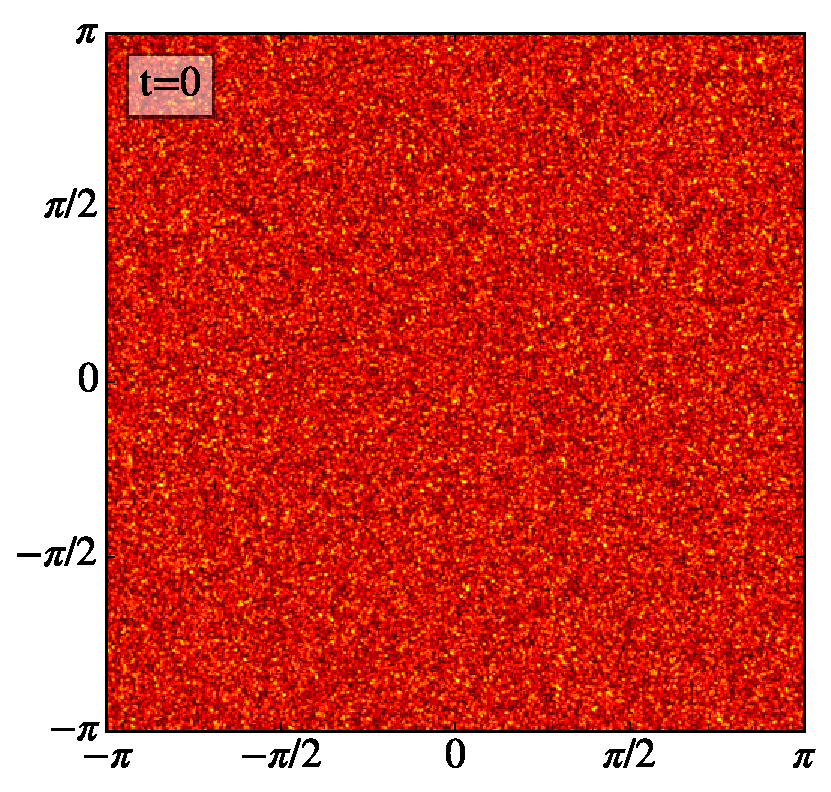
\includegraphics[width=0.49\textwidth]{helical_bb_slice_t0.pdf}}
		  \subcaptionbox{helical at $t=100$}
		  {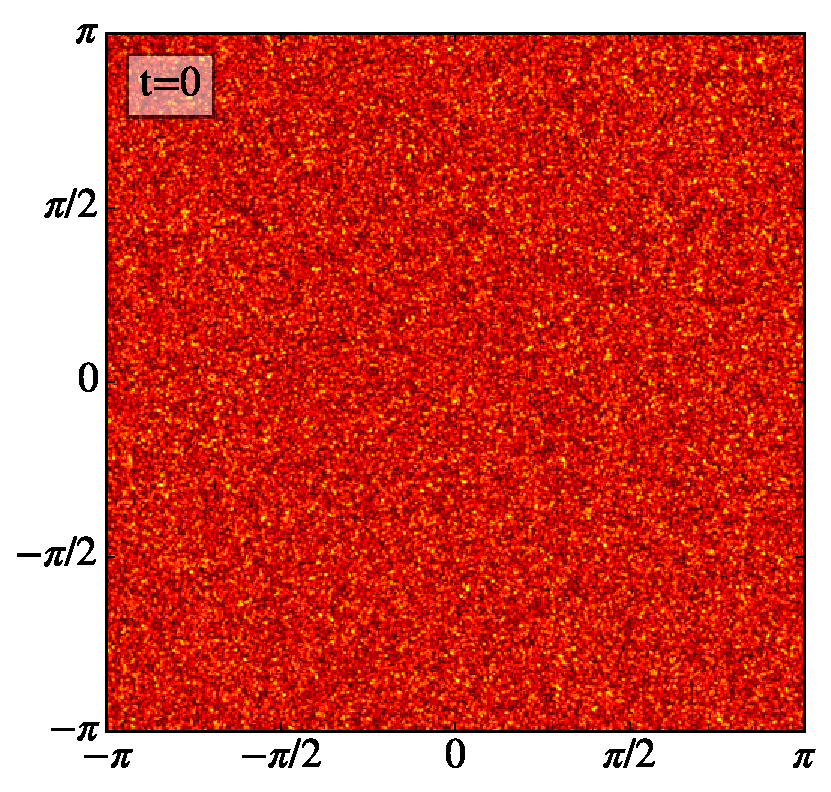
\includegraphics[width=0.49\textwidth]{helical_bb_slice_t100.pdf}}
                    \label{Fig:helical}
                  \caption{Slices of the run with $\mathcal{H}=\mathcal{H}_\textrm{max}$}
                \end{figure}

            \item Tables and graphics may appear in the text or in
                the appendix, especially if there are many simulation results
                tabulated, but is also depends on the study and number of tables resp.
                figures. The key graphs and tables must appear in
                the text!
        \end{itemize}

    \item Latex is really good at rendering formulas:\\
        \textit{Equation (\ref{Eq:SpecDens}) represents the ACs of a stationary
        stochastic process:
        \begin{equation}
            f_y(\lambda) = (2\pi)^{-1} \sum_{j=-\infty}^{\infty}
                           \gamma_j e^{-i\lambda j}
                         =(2\pi)^{-1}\left(\gamma_0 + 2 \sum_{j=1}^{\infty}
        \gamma_j \cos(\lambda j)\right)
                                        \label{Eq:SpecDens}
        \end{equation}
        where $i=\sqrt{-1}$ is the imaginary unit, $\lambda \in [-\pi,
        \pi]$ is the frequency and the $\gamma_j$ are the autocovariances
        of $y_t$.}

\newpage

    \item Discuss results:
        \begin{itemize}
            \item Do the results support or do they contradict economic theory ?
            \item What does the reader learn from the results?
            \item Try to give an intuition for your results.
            \item Provide robustness checks.
            \item Compare to previous research.
        \end{itemize}
\end{itemize}

\newpage
\chapter{Conclusions}\label{Chap:Conc}

\begin{itemize}

    \item Give a short summary of what has been done and what has been
    found.

    \item Expose results concisely.

    \item Draw conclusions about the problem studied. What are the
    implications of your findings?

    \item Point out some limitations of study (assist reader in judging validity
    of findings).

    \item Suggest issues for future research.

\end{itemize}




% ----------------
% --- appendix ---
% ----------------
\appendix

% literature
\newpage
\addcontentsline{toc}{chapter}{References}
\bibliography{astro_johannes}

% --------------------------------------------
% --- last page: Declaration of Authorship ---
% --------------------------------------------

\newpage
\thispagestyle{empty}
%{\Large{\bf Declaration of Authorship}}\vspace{0.5cm}

\section*{Declaration of Authorship}

I hereby confirm that I have authored this thesis independently and without use of others than the indicated
sources. All passages which are literally or in general matter
taken out of publications or other sources are marked as such.
\vspace{1cm}

Hamburg, January 1 \vspace{0.5cm}

Johannes Reppin


\end{document}
